\documentclass[
    11pt,
    a4paper,
    egregdoesnotlikesansseriftitles,
    toc=chapterentrywithdots,
    twoside,openright,
    titlepage,
    parskip=half,
    headings=normal,  % reduces heading size
    listof=totoc,
    bibliography=totoc,
    index=totoc,
    captions=tableheading,  % caption below table
    chapterprefix,
    listof=flat,
    final,
    pointlessnumbers
]{scrbook}


% details about your thesis
\newcommand{\titel}{Analyse und Bewertung von Methoden zur Sicherung der Vertraulichkeit in Neuronalen Netzen}
\newcommand{\titelEN}{Analysis and Evaluation of Methods for Ensuring Confidentiality in Neural Networks}
\newcommand{\artderarbeit}{Masterarbeit}  % {Bachelorarbeit,Masterarbeit}
\newcommand{\autor}{Sabau Patrick}
\newcommand{\studiengang}{Künstliche Intelligenz}  % {Informatik,Wirtschaftsinformatik,Medieninformatik}
\newcommand{\matrikelnr}{12913724}
\newcommand{\erstgutachter}{{Prof.\,Dr.-Ing.~Christoph P. Neumann}}
\newcommand{\zweitgutachter}{{Prof.\,Dr. rer. nat.~Daniel Loebenberger}}
\newcommand{\betreuer}{}
\newcommand{\unternehmen}{}
\newcommand{\logo}{figures/TH-Nuernberg-RGB.png}
\newcommand{\keywords}{machine, learning}
 

% custom head and foot
\usepackage[automark]{scrlayer-scrpage}
\pagestyle{scrheadings}
\ihead{\headmark}
\chead{}
\ohead{\pagemark}
\renewcommand*\chaptermarkformat{\chapappifchapterprefix{\ }% 
  \thechapter.\enskip}




% \RedeclareSectionCommand[tocindent=0pt]{section}
% \RedeclareSectionCommand[tocindent=0pt]{subsection}
% \RedeclareSectionCommand[tocnumwidth=70pt]{chapter}

\usepackage{scrhack}

% other packages
\usepackage[T1]{fontenc}
\usepackage[utf8]{inputenc}
\usepackage{lmodern,relsize,textcomp,csquotes}
\usepackage{amsmath,amsfonts}
\usepackage[ngerman]{babel} 
\usepackage[final]{graphicx}
\usepackage{setspace,geometry}
\usepackage[pdftex,cmyk,fixpdftex,hyperref,table,xcdraw]{xcolor}
\usepackage{makeidx}
\usepackage{paralist,ifthen,todonotes}
\usepackage{url}
\usepackage[toc]{glossaries}
\usepackage{pdfpages}
\usepackage{amsmath}
\usepackage{multirow}

%\usepackage{emptypage}

% table setup
\usepackage{longtable}
\usepackage{array}
\usepackage{ragged2e}
\usepackage{lscape}

% pdf hyperref
\usepackage[
    bookmarks=true,
    bookmarksopen=true,
    bookmarksnumbered=true,
    bookmarksopenlevel=1,
    pdftitle={\titel},
    pdfauthor={\autor},
    pdfcreator={\autor},
    pdfsubject={\titel},
    pdfkeywords={\keywords},
    pdfpagelabels=true,
    colorlinks=true,
    linkcolor=red,
    urlcolor=magenta,
    anchorcolor=black,
    citecolor=cyan,
    filecolor=magenta,
    menucolor=red,
    plainpages=false,
    hypertexnames=true,
    linktocpage=true,
]{hyperref}


% configure your listings style
\usepackage{listings}
\lstset{
	tabsize=3,
	extendedchars=true,
	frame=single,
	showstringspaces=true,
	numbers=left,
	numberstyle=\small,
	breakautoindent=true
}

\usepackage[
    backend=biber,
    style=ieee,
    natbib=true,
    url=false,
    doi=false,
    eprint=false
]{biblatex}
\addbibresource{refs.bib}

% page setup
% \setlength{\topskip}{\ht\strutbox}
\geometry{paper=a4paper,left=2.5cm,top=3.0cm,bindingoffset=.8cm}
\onehalfspacing
\frenchspacing
\clubpenalty = 10000
\widowpenalty = 10000 
\displaywidowpenalty = 10000

% some commands
\newcommand{\ua}{\mbox{u.\,a.\ }}
\newcommand{\zB}{\mbox{z.\,B.\ }}
\newcommand{\dahe}{\mbox{d.\,h.,\ }}
\newcommand{\bzw}{\mbox{bzw.\ }}
\newcommand{\bzgl}{\mbox{bzgl.\ }}
\newcommand{\eg}{\mbox{e.\,g.\ }}
\newcommand{\ie}{\mbox{i.\,e.\ }}
\newcommand{\wrt}{\mbox{w.\,r.\,t.\ }}
\newcommand{\etal}{\mbox{\emph{et.\,al.\ }}}



\begin{document}

\setcounter{secnumdepth}{3}  % numerate subsections
\setcounter{tocdepth}{2}  % ...but don't include them in toc

\frontmatter

\thispagestyle{empty}
\pdfbookmark[1]{Cover}{cov}
\begin{titlepage}

\begin{center}


\includegraphics[width=7cm]{figures/Hochschule_Amberg-Weiden_Logo_2013.png}\\[1cm]
% \begin{tikzpicture}[y=0.80pt, x=0.8pt,yscale=-0.35,xscale=0.35, inner sep=0pt, outer sep=0pt]
\begin{scope}[cm={{1.25,0.0,0.0,-1.25,(0.0,259.45)}}]
  \begin{scope}[scale=0.100]
    \path[fill=ca69788,nonzero rule] (104.9570,451.7810) .. controls
      (102.2700,460.3200) and (93.2422,473.2500) .. (75.1836,473.2500) .. controls
      (63.7188,473.2500) and (53.7148,467.3910) .. (48.8398,458.3590) .. controls
      (42.9844,447.3910) and (40.2969,432.5000) .. (40.2969,412.0120) .. controls
      (40.2969,382.7300) and (45.1758,364.4300) .. (55.4258,357.1090) .. controls
      (60.7891,353.2110) and (67.6211,351.2500) .. (75.6719,351.2500) .. controls
      (99.3398,351.2500) and (109.3480,369.3090) .. (109.3480,412.5000) .. controls
      (109.3480,429.8200) and (107.8830,442.2620) .. (104.9570,451.7810) --
      cycle(110.8130,332.9490) .. controls (100.5630,327.3400) and
      (91.0430,325.1480) .. (76.8945,325.1480) .. controls (51.2734,325.1480) and
      (34.6875,332.2190) .. (21.7539,349.0590) .. controls (8.8242,365.6480) and
      (2.2383,387.1210) .. (2.2383,412.0120) .. controls (2.2383,448.6090) and
      (16.1445,477.8910) .. (40.5430,491.3010) .. controls (50.5469,496.6720) and
      (62.9883,499.6020) .. (75.6719,499.6020) .. controls (120.8160,499.6020) and
      (148.6290,466.6600) .. (148.6290,413.4690) .. controls (148.6290,375.1720) and
      (135.4530,346.3790) .. (110.8130,332.9490);
    \path[fill=ca69788,nonzero rule] (213.7770,323.9300) .. controls
      (198.4060,323.9300) and (181.5700,328.8090) .. (163.2700,338.3320) --
      (174.9840,362.2380) .. controls (184.9840,356.1290) and (202.3090,348.0820) ..
      (216.4610,348.0820) .. controls (225.7300,348.0820) and (233.0510,354.1800) ..
      (233.0510,362.2380) .. controls (233.0510,370.7810) and (226.9530,375.1720) ..
      (213.7770,377.6090) -- (199.1410,380.2890) .. controls (190.8440,381.7500) and
      (180.5980,387.6090) .. (176.2070,392.9800) .. controls (171.8130,398.3400) and
      (169.1250,407.3710) .. (169.1250,415.4220) .. controls (169.1250,439.8200) and
      (188.4020,456.1720) .. (217.4380,456.1720) .. controls (237.4450,456.1720) and
      (250.6210,450.0700) .. (262.0900,444.4610) -- (251.3520,422.5000) .. controls
      (238.9100,428.8400) and (229.8830,431.5310) .. (220.6090,431.5310) .. controls
      (211.0940,431.5310) and (204.7500,426.6480) .. (204.7500,419.3320) .. controls
      (204.7500,412.9800) and (208.8950,409.5700) .. (220.3670,406.6410) --
      (235.4920,402.7300) .. controls (250.8630,398.8320) and (255.9840,394.1910) ..
      (260.3830,388.5820) .. controls (265.0160,382.7300) and (267.2110,375.6480) ..
      (267.2110,367.3590) .. controls (267.2110,341.4880) and (245.7420,323.9300) ..
      (213.7770,323.9300);
    \path[fill=ca69788,nonzero rule] (329.8950,324.8980) .. controls
      (313.3010,324.8980) and (300.1290,332.2190) .. (296.2270,343.1990) .. controls
      (294.2730,348.5700) and (294.0270,351.0120) .. (294.0270,362.4800) --
      (294.0270,430.3090) -- (281.5820,430.3090) -- (281.5820,452.7500) --
      (294.0270,452.7500) .. controls (294.0270,464.9490) and (294.0270,473.0000) ..
      (295.2500,482.2810) -- (328.4300,490.5700) .. controls (327.2110,479.1090) and
      (326.4800,465.4410) .. (326.4800,452.7500) -- (355.7580,452.7500) --
      (347.4610,430.3090) -- (326.4800,430.3090) -- (326.4800,367.6020) .. controls
      (326.4800,351.7380) and (329.4020,347.5900) .. (340.6290,347.5900) .. controls
      (343.5550,347.5900) and (346.4840,348.3320) .. (352.3400,350.0310) --
      (356.4880,330.5200) .. controls (346.9730,326.6090) and (338.4340,324.8980) ..
      (329.8950,324.8980);
    \path[fill=ca69788,nonzero rule] (447.7380,412.9800) .. controls
      (445.2970,423.7190) and (438.4690,428.8400) .. (429.9260,428.8400) .. controls
      (421.3870,428.8400) and (415.5310,423.4800) .. (411.3870,418.8400) --
      (411.3870,361.2620) .. controls (415.7770,357.3520) and (420.8980,353.2110) ..
      (429.6840,353.2110) .. controls (437.7340,353.2110) and (442.8590,356.3790) ..
      (445.5430,362.9610) .. controls (448.4730,369.8010) and (449.2030,376.3910) ..
      (449.2030,391.7620) .. controls (449.2030,402.9800) and (448.9610,407.6210) ..
      (447.7380,412.9800) -- cycle(463.1090,335.1480) .. controls
      (454.5700,328.3200) and (446.0310,325.3910) .. (435.7810,325.3910) .. controls
      (423.5860,325.3910) and (415.0430,329.0510) .. (407.9690,336.8590) .. controls
      (406.9920,332.4690) and (406.7460,331.2500) .. (404.5510,327.8320) --
      (375.2730,327.8320) .. controls (377.7150,333.4410) and (378.4450,337.1020) ..
      (378.4450,354.4300) -- (378.4450,470.0820) .. controls (378.4450,485.4490) and
      (377.9610,493.7500) .. (376.2500,500.8200) -- (409.6800,508.6290) .. controls
      (410.6520,500.0900) and (410.8980,494.9690) .. (410.8980,486.4300) --
      (410.8980,456.8980) .. controls (410.8980,453.2380) and (410.6520,447.8790) ..
      (410.1680,445.9220) .. controls (416.5080,452.7500) and (425.2930,455.9300) ..
      (436.7580,455.9300) .. controls (467.2580,455.9300) and (486.2890,431.5310) ..
      (486.2890,392.4920) .. controls (486.2890,367.1090) and (478.4800,347.3520) ..
      (463.1090,335.1480);
    \path[fill=ca69788,nonzero rule] (572.3870,382.4920) .. controls
      (549.6910,382.4920) and (541.8870,378.3400) .. (541.8870,363.4490) .. controls
      (541.8870,353.6990) and (547.9880,347.1090) .. (556.2850,347.1090) .. controls
      (562.3830,347.1090) and (568.4800,350.2810) .. (573.3590,355.6410) --
      (573.8480,382.4920) -- (572.3870,382.4920) -- cycle(600.1990,321.4880) ..
      controls (592.6370,324.6600) and (585.8050,330.2700) .. (582.6330,336.6210) ..
      controls (580.1950,334.1720) and (577.5120,331.7300) .. (575.0660,330.0310) ..
      controls (568.9690,325.6290) and (560.1880,323.1990) .. (549.9380,323.1990) ..
      controls (522.1250,323.1990) and (506.9960,337.3520) .. (506.9960,362.2380) ..
      controls (506.9960,391.5120) and (527.2460,405.1800) .. (567.0160,405.1800) ..
      controls (569.4570,405.1800) and (571.6560,405.1800) .. (574.3360,404.9300) --
      (574.3360,410.0510) .. controls (574.3360,423.9610) and (571.6560,428.6020) ..
      (559.6950,428.6020) .. controls (549.2030,428.6020) and (537.0080,423.4800) ..
      (523.5900,414.4490) -- (509.6840,437.8710) .. controls (516.2700,442.0200) and
      (521.1480,444.4610) .. (529.9340,448.1210) .. controls (542.1290,453.2380) and
      (552.6210,455.4410) .. (564.0940,455.4410) .. controls (585.0740,455.4410) and
      (599.4690,447.6290) .. (604.3480,433.7190) .. controls (606.0550,428.6020) and
      (606.7850,424.6990) .. (606.5430,411.2700) -- (605.8130,369.3090) .. controls
      (605.5660,355.6410) and (606.5430,349.7890) .. (617.5230,341.4880) --
      (600.1990,321.4880);
    \path[fill=ca69788,nonzero rule] (702.8910,325.8790) .. controls
      (694.3520,301.7190) and (688.0080,291.2420) .. (678.9800,284.6480) .. controls
      (670.6840,278.5510) and (659.9490,274.6410) .. (648.7270,273.1800) --
      (637.5040,294.6480) .. controls (644.5780,296.6020) and (652.8750,299.5310) ..
      (657.7540,302.9410) .. controls (661.4100,305.6290) and (664.3400,309.0390) ..
      (667.0270,313.1910) .. controls (670.1950,318.3200) and (671.1720,320.5120) ..
      (674.1020,327.8320) -- (665.8050,327.8320) .. controls (661.8980,339.5510) and
      (655.3130,359.0590) .. (654.0940,362.9610) -- (624.5700,450.8010) --
      (657.9960,454.7110) -- (679.7110,381.7500) .. controls (681.6640,374.4300) and
      (685.8130,357.6020) .. (686.3010,355.8910) .. controls (686.3010,356.6210) and
      (688.7380,369.8010) .. (690.2030,375.8980) .. controls (691.1840,380.0390) and
      (693.1290,387.3590) .. (695.0820,393.2190) -- (713.8710,452.7500) --
      (748.2700,452.7500) -- (702.8910,325.8790);
    \path[fill=ca69788,nonzero rule] (832.9100,405.4220) .. controls
      (832.9100,414.6910) and (831.9340,419.5700) .. (829.0080,424.2110) .. controls
      (825.8360,429.0900) and (821.1990,431.5310) .. (814.6130,431.5310) .. controls
      (802.1680,431.5310) and (795.0940,421.7700) .. (795.0940,404.4410) --
      (795.0940,403.9610) -- (832.9100,403.9610) -- (832.9100,405.4220) --
      cycle(794.6050,380.0390) -- (794.6050,379.0700) .. controls
      (794.6050,359.8010) and (804.1210,348.8090) .. (820.9570,348.8090) .. controls
      (832.1800,348.8090) and (842.6720,352.9610) .. (852.6760,361.2620) --
      (865.3590,341.7380) .. controls (850.9690,330.0310) and (835.8400,324.4100) ..
      (818.2700,324.4100) .. controls (782.4060,324.4100) and (759.2300,349.7890) ..
      (759.2300,389.0700) .. controls (759.2300,411.5200) and (763.8630,426.3980) ..
      (774.8440,438.6020) .. controls (785.0900,450.0700) and (797.5350,455.4410) ..
      (814.1250,455.4410) .. controls (828.5200,455.4410) and (842.1840,450.5590) ..
      (850.2340,442.2620) .. controls (861.7030,430.5510) and (866.8240,413.7190) ..
      (866.8240,387.6090) -- (866.8240,380.0390) -- (794.6050,380.0390);
    \path[fill=ca69788,nonzero rule] (955.8910,424.2110) .. controls
      (952.7150,425.9100) and (950.0350,426.6480) .. (946.3710,426.6480) .. controls
      (939.0550,426.6480) and (932.4650,423.2300) .. (926.3670,416.1600) --
      (926.3670,327.8320) -- (893.6720,327.8320) -- (893.6720,411.2700) .. controls
      (893.6720,428.1090) and (891.7190,440.8010) .. (889.0310,447.8790) --
      (918.3160,455.6800) .. controls (921.2380,450.5590) and (922.9490,444.9490) ..
      (923.4380,437.8710) .. controls (930.5120,447.3910) and (940.5200,455.6800) ..
      (952.7150,455.6800) .. controls (957.5980,455.6800) and (959.7890,455.1990) ..
      (964.9180,453.0000) -- (955.8910,424.2110);
    \path[fill=ca69788,nonzero rule] (981.9920,327.8320) -- (981.9920,450.5590) --
      (1014.6900,455.6800) -- (1014.6900,327.8320) -- (981.9920,327.8320) --
      cycle(998.3400,466.8980) .. controls (987.3590,466.8980) and
      (978.3280,475.9300) .. (978.3280,487.1600) .. controls (978.3280,498.3790) and
      (987.6020,507.4100) .. (998.8280,507.4100) .. controls (1009.8000,507.4100)
      and (1018.5900,498.3790) .. (1018.5900,487.1600) .. controls
      (1018.5900,475.9300) and (1009.5600,466.8980) .. (998.3400,466.8980);
    \path[fill=ca69788,nonzero rule] (1089.5900,323.9300) .. controls
      (1074.2200,323.9300) and (1057.3800,328.8090) .. (1039.0800,338.3320) --
      (1050.8000,362.2380) .. controls (1060.8000,356.1290) and (1078.1200,348.0820)
      .. (1092.2700,348.0820) .. controls (1101.5400,348.0820) and
      (1108.8600,354.1800) .. (1108.8600,362.2380) .. controls (1108.8600,370.7810)
      and (1102.7600,375.1720) .. (1089.5900,377.6090) -- (1074.9500,380.2890) ..
      controls (1066.6600,381.7500) and (1056.4100,387.6090) .. (1052.0200,392.9800)
      .. controls (1047.6200,398.3400) and (1044.9400,407.3710) ..
      (1044.9400,415.4220) .. controls (1044.9400,439.8200) and (1064.2100,456.1720)
      .. (1093.2500,456.1720) .. controls (1113.2600,456.1720) and
      (1126.4300,450.0700) .. (1137.9000,444.4610) -- (1127.1600,422.5000) ..
      controls (1114.7200,428.8400) and (1105.6900,431.5310) .. (1096.4200,431.5310)
      .. controls (1086.9000,431.5310) and (1080.5600,426.6480) ..
      (1080.5600,419.3320) .. controls (1080.5600,412.9800) and (1084.7100,409.5700)
      .. (1096.1800,406.6410) -- (1111.3000,402.7300) .. controls
      (1126.6700,398.8320) and (1131.8000,394.1910) .. (1136.1900,388.5820) ..
      controls (1140.8300,382.7300) and (1143.0200,375.6480) .. (1143.0200,367.3590)
      .. controls (1143.0200,341.4880) and (1121.5500,323.9300) ..
      (1089.5900,323.9300);
    \path[fill=ca69788,nonzero rule] (1247.4200,332.7110) .. controls
      (1238.6300,327.5900) and (1228.8700,324.8980) .. (1216.9200,324.8980) ..
      controls (1182.5100,324.8980) and (1162.5100,348.8090) .. (1162.5100,389.3200)
      .. controls (1162.5100,418.1090) and (1173.4900,437.1410) ..
      (1188.1300,447.1410) .. controls (1196.4200,452.7500) and (1208.6200,456.4220)
      .. (1219.1200,456.4220) .. controls (1227.4100,456.4220) and
      (1236.4400,454.4610) .. (1243.2700,450.8010) .. controls (1247.9100,448.3590)
      and (1250.1000,446.6600) .. (1255.4700,442.0200) -- (1239.6100,420.5510) ..
      controls (1233.0200,426.6480) and (1225.9500,430.3090) .. (1219.8400,430.3090)
      .. controls (1205.2100,430.3090) and (1198.6200,417.6210) ..
      (1198.6200,388.3400) .. controls (1198.6200,371.9880) and (1200.8200,362.2380)
      .. (1204.9600,356.8710) .. controls (1208.3800,352.4800) and
      (1213.9900,349.7890) .. (1219.6000,349.7890) .. controls (1227.1600,349.7890)
      and (1234.0000,352.9610) .. (1242.0500,360.0390) -- (1244.0000,361.7500) --
      (1258.8800,341.9800) .. controls (1254.0000,337.1020) and (1251.8100,335.3980)
      .. (1247.4200,332.7110);
    \path[fill=ca69788,nonzero rule] (1350.1100,327.8320) -- (1350.1100,411.7620) ..
      controls (1350.1100,424.2110) and (1346.6900,428.8400) .. (1337.4200,428.8400)
      .. controls (1329.3700,428.8400) and (1318.8800,423.9610) ..
      (1311.5600,417.3790) -- (1311.5600,327.8320) -- (1278.3700,327.8320) --
      (1278.3700,472.2700) .. controls (1278.3700,483.9800) and (1277.4000,495.6990)
      .. (1275.9300,500.8200) -- (1309.3600,508.6290) .. controls
      (1310.8300,501.8010) and (1311.5600,490.0820) .. (1311.5600,478.1290) --
      (1311.5600,453.2380) .. controls (1311.5600,449.3400) and (1311.0700,444.2110)
      .. (1311.0700,442.7500) .. controls (1319.6100,450.8010) and
      (1333.7600,456.1720) .. (1346.4500,456.1720) .. controls (1362.3000,456.1720)
      and (1374.9900,449.3400) .. (1378.9000,438.3590) .. controls
      (1381.3400,431.2810) and (1382.0700,427.1290) .. (1382.0700,415.1800) --
      (1382.0700,327.8320) -- (1350.1100,327.8320);
    \path[fill=ca69788,nonzero rule] (1486.2500,405.4220) .. controls
      (1486.2500,414.6910) and (1485.2700,419.5700) .. (1482.3500,424.2110) ..
      controls (1479.1700,429.0900) and (1474.5400,431.5310) .. (1467.9500,431.5310)
      .. controls (1455.5100,431.5310) and (1448.4300,421.7700) ..
      (1448.4300,404.4410) -- (1448.4300,403.9610) -- (1486.2500,403.9610) --
      (1486.2500,405.4220) -- cycle(1447.9400,380.0390) -- (1447.9400,379.0700) ..
      controls (1447.9400,359.8010) and (1457.4600,348.8090) .. (1474.3000,348.8090)
      .. controls (1485.5200,348.8090) and (1496.0100,352.9610) ..
      (1506.0200,361.2620) -- (1518.7000,341.7380) .. controls (1504.3100,330.0310)
      and (1489.1800,324.4100) .. (1471.6100,324.4100) .. controls
      (1435.7500,324.4100) and (1412.5700,349.7890) .. (1412.5700,389.0700) ..
      controls (1412.5700,411.5200) and (1417.2000,426.3980) .. (1428.1800,438.6020)
      .. controls (1438.4300,450.0700) and (1450.8700,455.4410) ..
      (1467.4700,455.4410) .. controls (1481.8600,455.4410) and (1495.5200,450.5590)
      .. (1503.5700,442.2620) .. controls (1515.0400,430.5510) and
      (1520.1700,413.7190) .. (1520.1700,387.6090) -- (1520.1700,380.0390) --
      (1447.9400,380.0390);
    \path[fill=ca69788,nonzero rule] (1702.6700,469.1020) -- (1662.1700,469.1020) --
      (1662.1700,327.8320) -- (1627.5200,327.8320) -- (1627.5200,469.1020) --
      (1586.0500,469.1020) -- (1586.0500,497.3980) -- (1708.2900,497.3980) --
      (1702.6700,469.1020);
    \path[fill=ca69788,nonzero rule] (1770.9800,405.4220) .. controls
      (1770.9800,414.6910) and (1770.0000,419.5700) .. (1767.0800,424.2110) ..
      controls (1763.9000,429.0900) and (1759.2600,431.5310) .. (1752.6800,431.5310)
      .. controls (1740.2400,431.5310) and (1733.1600,421.7700) ..
      (1733.1600,404.4410) -- (1733.1600,403.9610) -- (1770.9800,403.9610) --
      (1770.9800,405.4220) -- cycle(1732.6700,380.0390) -- (1732.6700,379.0700) ..
      controls (1732.6700,359.8010) and (1742.1900,348.8090) .. (1759.0200,348.8090)
      .. controls (1770.2500,348.8090) and (1780.7400,352.9610) ..
      (1790.7400,361.2620) -- (1803.4300,341.7380) .. controls (1789.0300,330.0310)
      and (1773.9000,324.4100) .. (1756.3400,324.4100) .. controls
      (1720.4700,324.4100) and (1697.2900,349.7890) .. (1697.2900,389.0700) ..
      controls (1697.2900,411.5200) and (1701.9300,426.3980) .. (1712.9100,438.6020)
      .. controls (1723.1600,450.0700) and (1735.6000,455.4410) ..
      (1752.1900,455.4410) .. controls (1766.5900,455.4410) and (1780.2500,450.5590)
      .. (1788.3100,442.2620) .. controls (1799.7700,430.5510) and
      (1804.8900,413.7190) .. (1804.8900,387.6090) -- (1804.8900,380.0390) --
      (1732.6700,380.0390);
    \path[fill=ca69788,nonzero rule] (1909.3300,332.7110) .. controls
      (1900.5500,327.5900) and (1890.7900,324.8980) .. (1878.8300,324.8980) ..
      controls (1844.4300,324.8980) and (1824.4200,348.8090) .. (1824.4200,389.3200)
      .. controls (1824.4200,418.1090) and (1835.4100,437.1410) ..
      (1850.0400,447.1410) .. controls (1858.3300,452.7500) and (1870.5300,456.4220)
      .. (1881.0300,456.4220) .. controls (1889.3200,456.4220) and
      (1898.3500,454.4610) .. (1905.1800,450.8010) .. controls (1909.8200,448.3590)
      and (1912.0200,446.6600) .. (1917.3800,442.0200) -- (1901.5200,420.5510) ..
      controls (1894.9400,426.6480) and (1887.8600,430.3090) .. (1881.7600,430.3090)
      .. controls (1867.1200,430.3090) and (1860.5300,417.6210) ..
      (1860.5300,388.3400) .. controls (1860.5300,371.9880) and (1862.7300,362.2380)
      .. (1866.8800,356.8710) .. controls (1870.2900,352.4800) and
      (1875.9000,349.7890) .. (1881.5200,349.7890) .. controls (1889.0800,349.7890)
      and (1895.9100,352.9610) .. (1903.9600,360.0390) -- (1905.9100,361.7500) --
      (1920.8000,341.9800) .. controls (1915.9200,337.1020) and (1913.7300,335.3980)
      .. (1909.3300,332.7110);
    \path[fill=ca69788,nonzero rule] (2012.0200,327.8320) -- (2012.0200,411.7620) ..
      controls (2012.0200,424.2110) and (2008.6100,428.8400) .. (1999.3300,428.8400)
      .. controls (1991.2800,428.8400) and (1980.7900,423.9610) ..
      (1973.4700,417.3790) -- (1973.4700,327.8320) -- (1940.2900,327.8320) --
      (1940.2900,472.2700) .. controls (1940.2900,483.9800) and (1939.3100,495.6990)
      .. (1937.8500,500.8200) -- (1971.2700,508.6290) .. controls
      (1972.7400,501.8010) and (1973.4700,490.0820) .. (1973.4700,478.1290) --
      (1973.4700,453.2380) .. controls (1973.4700,449.3400) and (1972.9800,444.2110)
      .. (1972.9800,442.7500) .. controls (1981.5200,450.8010) and
      (1995.6700,456.1720) .. (2008.3600,456.1720) .. controls (2024.2200,456.1720)
      and (2036.9100,449.3400) .. (2040.8100,438.3590) .. controls
      (2043.2500,431.2810) and (2043.9800,427.1290) .. (2043.9800,415.1800) --
      (2043.9800,327.8320) -- (2012.0200,327.8320);
    \path[fill=ca69788,nonzero rule] (2148.1600,327.8320) -- (2148.1600,409.0820) ..
      controls (2148.1600,423.2300) and (2145.7300,427.3790) .. (2137.1800,427.3790)
      .. controls (2130.6000,427.3790) and (2122.0600,422.9880) ..
      (2114.5000,416.1600) -- (2114.5000,327.8320) -- (2081.8000,327.8320) --
      (2081.8000,418.3520) .. controls (2081.8000,429.0900) and (2080.3400,439.3400)
      .. (2077.4100,447.6290) -- (2106.4400,455.9300) .. controls
      (2109.3700,450.8010) and (2111.0800,445.4300) .. (2111.0800,440.3090) ..
      controls (2115.9600,443.7300) and (2120.1000,446.6600) .. (2125.4700,449.5820)
      .. controls (2132.0700,453.0000) and (2140.6000,454.9490) ..
      (2147.9300,454.9490) .. controls (2161.8400,454.9490) and (2174.0200,447.6290)
      .. (2177.9300,436.8910) .. controls (2179.6500,432.2620) and
      (2180.3700,426.8910) .. (2180.3700,419.0820) -- (2180.3700,327.8320) --
      (2148.1600,327.8320);
    \path[fill=ca69788,nonzero rule] (2218.2000,327.8320) -- (2218.2000,450.5590) --
      (2250.9000,455.6800) -- (2250.9000,327.8320) -- (2218.2000,327.8320) --
      cycle(2234.5500,466.8980) .. controls (2223.5700,466.8980) and
      (2214.5300,475.9300) .. (2214.5300,487.1600) .. controls (2214.5300,498.3790)
      and (2223.8100,507.4100) .. (2235.0400,507.4100) .. controls
      (2246.0200,507.4100) and (2254.8000,498.3790) .. (2254.8000,487.1600) ..
      controls (2254.8000,475.9300) and (2245.7600,466.8980) ..
      (2234.5500,466.8980);
    \path[fill=ca69788,nonzero rule] (2325.7800,323.9300) .. controls
      (2310.4100,323.9300) and (2293.5700,328.8090) .. (2275.2900,338.3320) --
      (2286.9900,362.2380) .. controls (2296.9900,356.1290) and (2314.3200,348.0820)
      .. (2328.4800,348.0820) .. controls (2337.7500,348.0820) and
      (2345.0600,354.1800) .. (2345.0600,362.2380) .. controls (2345.0600,370.7810)
      and (2338.9600,375.1720) .. (2325.7800,377.6090) -- (2311.1500,380.2890) ..
      controls (2302.8500,381.7500) and (2292.6000,387.6090) .. (2288.2200,392.9800)
      .. controls (2283.8300,398.3400) and (2281.1300,407.3710) ..
      (2281.1300,415.4220) .. controls (2281.1300,439.8200) and (2300.4100,456.1720)
      .. (2329.4500,456.1720) .. controls (2349.4500,456.1720) and
      (2362.6400,450.0700) .. (2374.1000,444.4610) -- (2363.3600,422.5000) ..
      controls (2350.9200,428.8400) and (2341.8900,431.5310) .. (2332.6200,431.5310)
      .. controls (2323.1100,431.5310) and (2316.7600,426.6480) ..
      (2316.7600,419.3320) .. controls (2316.7600,412.9800) and (2320.9200,409.5700)
      .. (2332.3800,406.6410) -- (2347.5000,402.7300) .. controls
      (2362.8700,398.8320) and (2368.0100,394.1910) .. (2372.3800,388.5820) ..
      controls (2377.0300,382.7300) and (2379.2200,375.6480) .. (2379.2200,367.3590)
      .. controls (2379.2200,341.4880) and (2357.7500,323.9300) ..
      (2325.7800,323.9300);
    \path[fill=ca69788,nonzero rule] (2483.6300,332.7110) .. controls
      (2474.8400,327.5900) and (2465.0800,324.8980) .. (2453.1300,324.8980) ..
      controls (2418.7300,324.8980) and (2398.7100,348.8090) .. (2398.7100,389.3200)
      .. controls (2398.7100,418.1090) and (2409.7100,437.1410) ..
      (2424.3400,447.1410) .. controls (2432.6400,452.7500) and (2444.8200,456.4220)
      .. (2455.3300,456.4220) .. controls (2463.6100,456.4220) and
      (2472.6600,454.4610) .. (2479.4700,450.8010) .. controls (2484.1200,448.3590)
      and (2486.3100,446.6600) .. (2491.6800,442.0200) -- (2475.8200,420.5510) ..
      controls (2469.2400,426.6480) and (2462.1500,430.3090) .. (2456.0500,430.3090)
      .. controls (2441.4300,430.3090) and (2434.8200,417.6210) ..
      (2434.8200,388.3400) .. controls (2434.8200,371.9880) and (2437.0300,362.2380)
      .. (2441.1700,356.8710) .. controls (2444.5900,352.4800) and
      (2450.2000,349.7890) .. (2455.8200,349.7890) .. controls (2463.3800,349.7890)
      and (2470.2100,352.9610) .. (2478.2600,360.0390) -- (2480.2100,361.7500) --
      (2495.1000,341.9800) .. controls (2490.2100,337.1020) and (2488.0300,335.3980)
      .. (2483.6300,332.7110);
    \path[fill=ca69788,nonzero rule] (2586.3100,327.8320) -- (2586.3100,411.7620) ..
      controls (2586.3100,424.2110) and (2582.9100,428.8400) .. (2573.6300,428.8400)
      .. controls (2565.5900,428.8400) and (2555.0800,423.9610) ..
      (2547.7700,417.3790) -- (2547.7700,327.8320) -- (2514.5900,327.8320) --
      (2514.5900,472.2700) .. controls (2514.5900,483.9800) and (2513.6100,495.6990)
      .. (2512.1500,500.8200) -- (2545.5700,508.6290) .. controls
      (2547.0300,501.8010) and (2547.7700,490.0820) .. (2547.7700,478.1290) --
      (2547.7700,453.2380) .. controls (2547.7700,449.3400) and (2547.2900,444.2110)
      .. (2547.2900,442.7500) .. controls (2555.8200,450.8010) and
      (2569.9600,456.1720) .. (2582.6600,456.1720) .. controls (2598.5200,456.1720)
      and (2611.2100,449.3400) .. (2615.1000,438.3590) .. controls
      (2617.5400,431.2810) and (2618.2800,427.1290) .. (2618.2800,415.1800) --
      (2618.2800,327.8320) -- (2586.3100,327.8320);
    \path[fill=ca69788,nonzero rule] (2722.4600,405.4220) .. controls
      (2722.4600,414.6910) and (2721.4800,419.5700) .. (2718.5500,424.2110) ..
      controls (2715.3900,429.0900) and (2710.7400,431.5310) .. (2704.1600,431.5310)
      .. controls (2691.7200,431.5310) and (2684.6500,421.7700) ..
      (2684.6500,404.4410) -- (2684.6500,403.9610) -- (2722.4600,403.9610) --
      (2722.4600,405.4220) -- cycle(2684.1600,380.0390) -- (2684.1600,379.0700) ..
      controls (2684.1600,359.8010) and (2693.6700,348.8090) .. (2710.5100,348.8090)
      .. controls (2721.7400,348.8090) and (2732.2300,352.9610) ..
      (2742.2300,361.2620) -- (2754.9200,341.7380) .. controls (2740.5100,330.0310)
      and (2725.3900,324.4100) .. (2707.8300,324.4100) .. controls
      (2671.9500,324.4100) and (2648.7700,349.7890) .. (2648.7700,389.0700) ..
      controls (2648.7700,411.5200) and (2653.4200,426.3980) .. (2664.3900,438.6020)
      .. controls (2674.6500,450.0700) and (2687.0900,455.4410) ..
      (2703.6700,455.4410) .. controls (2718.0700,455.4410) and (2731.7400,450.5590)
      .. (2739.7900,442.2620) .. controls (2751.2500,430.5510) and
      (2756.3700,413.7190) .. (2756.3700,387.6090) -- (2756.3700,380.0390) --
      (2684.1600,380.0390);
    \path[fill=ca69788,nonzero rule] (2924.5100,327.8320) -- (2924.5100,403.4690) --
      (2875.7000,403.4690) -- (2875.7000,327.8320) -- (2841.8000,327.8320) --
      (2841.8000,497.3980) -- (2875.7000,497.3980) -- (2875.7000,431.5310) --
      (2924.5100,431.5310) -- (2924.5100,497.3980) -- (2959.1400,497.3980) --
      (2959.1400,327.8320) -- (2924.5100,327.8320);
    \path[fill=ca69788,nonzero rule] (3059.2000,424.4490) .. controls
      (3056.0200,428.6020) and (3050.9000,431.0390) .. (3045.0400,431.0390) ..
      controls (3037.2300,431.0390) and (3030.9000,426.1600) .. (3028.2000,418.3520)
      .. controls (3026.0200,411.7620) and (3024.7900,402.9800) ..
      (3024.7900,390.5390) .. controls (3024.7900,376.1410) and (3026.2500,365.4100)
      .. (3028.9500,359.0590) .. controls (3031.8800,352.2300) and
      (3039.1800,348.8090) .. (3045.5300,348.8090) .. controls (3059.6900,348.8090)
      and (3065.7800,361.5000) .. (3065.7800,391.0310) .. controls
      (3065.7800,407.8590) and (3063.5900,418.8400) .. (3059.2000,424.4490) --
      cycle(3085.7800,342.4690) .. controls (3076.2700,331.7300) and
      (3063.8300,325.1480) .. (3044.5500,325.1480) .. controls (3010.6400,325.1480)
      and (2988.4400,350.5200) .. (2988.4400,389.8010) .. controls
      (2988.4400,429.0900) and (3010.8800,455.1990) .. (3044.5500,455.1990) ..
      controls (3062.3600,455.1990) and (3076.2700,449.0900) .. (3087.0100,436.4100)
      .. controls (3097.0100,424.6990) and (3101.4100,411.0310) ..
      (3101.4100,390.7810) .. controls (3101.4100,369.3090) and (3096.5200,354.6720)
      .. (3085.7800,342.4690);
    \path[fill=ca69788,nonzero rule] (3208.2600,332.7110) .. controls
      (3199.4700,327.5900) and (3189.7300,324.8980) .. (3177.7700,324.8980) ..
      controls (3143.3600,324.8980) and (3123.3600,348.8090) .. (3123.3600,389.3200)
      .. controls (3123.3600,418.1090) and (3134.3400,437.1410) ..
      (3148.9800,447.1410) .. controls (3157.2700,452.7500) and (3169.4700,456.4220)
      .. (3179.9600,456.4220) .. controls (3188.2600,456.4220) and
      (3197.2900,454.4610) .. (3204.1200,450.8010) .. controls (3208.7500,448.3590)
      and (3210.9600,446.6600) .. (3216.3100,442.0200) -- (3200.4500,420.5510) ..
      controls (3193.8700,426.6480) and (3186.8000,430.3090) .. (3180.7000,430.3090)
      .. controls (3166.0500,430.3090) and (3159.4700,417.6210) ..
      (3159.4700,388.3400) .. controls (3159.4700,371.9880) and (3161.6600,362.2380)
      .. (3165.8200,356.8710) .. controls (3169.2200,352.4800) and
      (3174.8400,349.7890) .. (3180.4500,349.7890) .. controls (3188.0100,349.7890)
      and (3194.8400,352.9610) .. (3202.8900,360.0390) -- (3204.8400,361.7500) --
      (3219.7300,341.9800) .. controls (3214.8600,337.1020) and (3212.6600,335.3980)
      .. (3208.2600,332.7110);
    \path[fill=ca69788,nonzero rule] (3310.9600,327.8320) -- (3310.9600,411.7620) ..
      controls (3310.9600,424.2110) and (3307.5400,428.8400) .. (3298.2600,428.8400)
      .. controls (3290.2100,428.8400) and (3279.7300,423.9610) ..
      (3272.4000,417.3790) -- (3272.4000,327.8320) -- (3239.2200,327.8320) --
      (3239.2200,472.2700) .. controls (3239.2200,483.9800) and (3238.2400,495.6990)
      .. (3236.7800,500.8200) -- (3270.2100,508.6290) .. controls
      (3271.6800,501.8010) and (3272.4000,490.0820) .. (3272.4000,478.1290) --
      (3272.4000,453.2380) .. controls (3272.4000,449.3400) and (3271.9100,444.2110)
      .. (3271.9100,442.7500) .. controls (3280.4500,450.8010) and
      (3294.6100,456.1720) .. (3307.3000,456.1720) .. controls (3323.1600,456.1720)
      and (3335.8400,449.3400) .. (3339.7500,438.3590) .. controls
      (3342.1900,431.2810) and (3342.9100,427.1290) .. (3342.9100,415.1800) --
      (3342.9100,327.8320) -- (3310.9600,327.8320);
    \path[fill=ca69788,nonzero rule] (3420.2700,323.9300) .. controls
      (3404.9000,323.9300) and (3388.0700,328.8090) .. (3369.7700,338.3320) --
      (3381.4800,362.2380) .. controls (3391.4800,356.1290) and (3408.8100,348.0820)
      .. (3422.9500,348.0820) .. controls (3432.2300,348.0820) and
      (3439.5500,354.1800) .. (3439.5500,362.2380) .. controls (3439.5500,370.7810)
      and (3433.4600,375.1720) .. (3420.2700,377.6090) -- (3405.6300,380.2890) ..
      controls (3397.3400,381.7500) and (3387.0900,387.6090) .. (3382.7000,392.9800)
      .. controls (3378.3000,398.3400) and (3375.6300,407.3710) ..
      (3375.6300,415.4220) .. controls (3375.6300,439.8200) and (3394.9000,456.1720)
      .. (3423.9300,456.1720) .. controls (3443.9500,456.1720) and
      (3457.1100,450.0700) .. (3468.5700,444.4610) -- (3457.8500,422.5000) ..
      controls (3445.4100,428.8400) and (3436.3700,431.5310) .. (3427.1100,431.5310)
      .. controls (3417.6000,431.5310) and (3411.2500,426.6480) ..
      (3411.2500,419.3320) .. controls (3411.2500,412.9800) and (3415.3900,409.5700)
      .. (3426.8600,406.6410) -- (3441.9900,402.7300) .. controls
      (3457.3600,398.8320) and (3462.4800,394.1910) .. (3466.8800,388.5820) ..
      controls (3471.5000,382.7300) and (3473.7100,375.6480) .. (3473.7100,367.3590)
      .. controls (3473.7100,341.4880) and (3452.2300,323.9300) ..
      (3420.2700,323.9300);
    \path[fill=ca69788,nonzero rule] (3578.1100,332.7110) .. controls
      (3569.3200,327.5900) and (3559.5700,324.8980) .. (3547.6200,324.8980) ..
      controls (3513.2000,324.8980) and (3493.2000,348.8090) .. (3493.2000,389.3200)
      .. controls (3493.2000,418.1090) and (3504.1800,437.1410) ..
      (3518.8300,447.1410) .. controls (3527.1100,452.7500) and (3539.3200,456.4220)
      .. (3549.8000,456.4220) .. controls (3558.1100,456.4220) and
      (3567.1300,454.4610) .. (3573.9600,450.8010) .. controls (3578.5900,448.3590)
      and (3580.8000,446.6600) .. (3586.1500,442.0200) -- (3570.2900,420.5510) ..
      controls (3563.7100,426.6480) and (3556.6400,430.3090) .. (3550.5500,430.3090)
      .. controls (3535.9000,430.3090) and (3529.3200,417.6210) ..
      (3529.3200,388.3400) .. controls (3529.3200,371.9880) and (3531.5000,362.2380)
      .. (3535.6600,356.8710) .. controls (3539.0600,352.4800) and
      (3544.6900,349.7890) .. (3550.2900,349.7890) .. controls (3557.8500,349.7890)
      and (3564.6900,352.9610) .. (3572.7300,360.0390) -- (3574.6900,361.7500) --
      (3589.5700,341.9800) .. controls (3584.7100,337.1020) and (3582.5000,335.3980)
      .. (3578.1100,332.7110);
    \path[fill=ca69788,nonzero rule] (3680.7800,327.8320) -- (3680.7800,411.7620) ..
      controls (3680.7800,424.2110) and (3677.3800,428.8400) .. (3668.1100,428.8400)
      .. controls (3660.0600,428.8400) and (3649.5500,423.9610) ..
      (3642.2500,417.3790) -- (3642.2500,327.8320) -- (3609.0600,327.8320) --
      (3609.0600,472.2700) .. controls (3609.0600,483.9800) and (3608.0900,495.6990)
      .. (3606.6200,500.8200) -- (3640.0400,508.6290) .. controls
      (3641.5000,501.8010) and (3642.2500,490.0820) .. (3642.2500,478.1290) --
      (3642.2500,453.2380) .. controls (3642.2500,449.3400) and (3641.7600,444.2110)
      .. (3641.7600,442.7500) .. controls (3650.2900,450.8010) and
      (3664.4300,456.1720) .. (3677.1300,456.1720) .. controls (3692.9900,456.1720)
      and (3705.6800,449.3400) .. (3709.5700,438.3590) .. controls
      (3712.0100,431.2810) and (3712.7500,427.1290) .. (3712.7500,415.1800) --
      (3712.7500,327.8320) -- (3680.7800,327.8320);
    \path[fill=ca69788,nonzero rule] (3831.5800,324.4100) .. controls
      (3827.4200,327.3400) and (3824.0000,331.4880) .. (3821.8200,336.6210) ..
      controls (3813.7700,328.8090) and (3802.0500,324.6600) .. (3788.8700,324.6600)
      .. controls (3771.3100,324.6600) and (3756.1900,332.9490) ..
      (3752.0300,344.9100) .. controls (3750.0800,350.5200) and (3749.3600,357.1090)
      .. (3749.3600,369.8010) -- (3749.3600,449.8200) -- (3781.5600,455.9300) --
      (3781.5600,375.6480) .. controls (3781.5600,364.4300) and (3782.5400,358.5700)
      .. (3784.2400,355.1600) .. controls (3785.9600,351.7380) and
      (3790.8200,349.3010) .. (3795.7000,349.3010) .. controls (3803.7500,349.3010)
      and (3813.5200,355.1600) .. (3815.9600,361.2620) -- (3815.9600,449.0900) --
      (3847.1900,455.6800) -- (3847.1900,360.2810) .. controls (3847.1900,351.9880)
      and (3849.8800,343.4490) .. (3854.7500,337.5900) -- (3831.5800,324.4100);
    \path[fill=ca69788,nonzero rule] (3915.7200,324.8980) .. controls
      (3901.8200,324.8980) and (3890.5900,331.4880) .. (3886.7000,341.9800) ..
      controls (3884.2600,348.3320) and (3883.7700,352.2300) .. (3883.7700,370.0390)
      -- (3883.7700,463.2500) .. controls (3883.7700,479.5900) and
      (3883.2800,489.5900) .. (3882.0500,500.8200) -- (3915.4900,508.3790) ..
      controls (3916.7000,501.5510) and (3917.1900,493.5000) .. (3917.1900,475.9300)
      -- (3917.1900,378.5820) .. controls (3917.1900,357.1090) and
      (3917.4400,354.1800) .. (3919.3900,350.7700) .. controls (3920.6100,348.5700)
      and (3923.2800,347.3520) .. (3925.9800,347.3520) .. controls
      (3927.1900,347.3520) and (3927.9300,347.3520) .. (3929.6300,347.8400) --
      (3935.2500,328.3200) .. controls (3929.6300,326.1210) and (3922.7900,324.8980)
      .. (3915.7200,324.8980);
    \path[fill=ca69788,nonzero rule] (4021.1100,405.4220) .. controls
      (4021.1100,414.6910) and (4020.1400,419.5700) .. (4017.2100,424.2110) ..
      controls (4014.0200,429.0900) and (4009.3900,431.5310) .. (4002.8100,431.5310)
      .. controls (3990.3700,431.5310) and (3983.2800,421.7700) ..
      (3983.2800,404.4410) -- (3983.2800,403.9610) -- (4021.1100,403.9610) --
      (4021.1100,405.4220) -- cycle(3982.7900,380.0390) -- (3982.7900,379.0700) ..
      controls (3982.7900,359.8010) and (3992.3000,348.8090) .. (4009.1400,348.8090)
      .. controls (4020.3700,348.8090) and (4030.8600,352.9610) ..
      (4040.8600,361.2620) -- (4053.5500,341.7380) .. controls (4039.1600,330.0310)
      and (4024.0200,324.4100) .. (4006.4600,324.4100) .. controls
      (3970.6100,324.4100) and (3947.4200,349.7890) .. (3947.4200,389.0700) ..
      controls (3947.4200,411.5200) and (3952.0500,426.3980) .. (3963.0300,438.6020)
      .. controls (3973.2800,450.0700) and (3985.7200,455.4410) ..
      (4002.3200,455.4410) .. controls (4016.7200,455.4410) and (4030.3700,450.5590)
      .. (4038.4400,442.2620) .. controls (4049.9000,430.5510) and
      (4055.0200,413.7190) .. (4055.0200,387.6090) -- (4055.0200,380.0390) --
      (3982.7900,380.0390);
    \path[fill=cf68712,nonzero rule] (1253.2400,150.5390) .. controls
      (1251.5300,158.3520) and (1246.4100,180.5510) .. (1246.4100,180.5510) ..
      controls (1246.4100,180.5510) and (1241.5300,160.5510) .. (1238.3600,147.8710)
      .. controls (1235.1900,135.6600) and (1232.9900,127.6090) ..
      (1229.3300,116.3910) -- (1262.5100,116.3910) .. controls (1262.5100,116.3910)
      and (1256.9000,134.1910) .. (1253.2400,150.5390) -- cycle(1282.7600,47.8320)
      -- (1270.8100,88.0820) -- (1221.0400,88.0820) -- (1209.0800,47.8320) --
      (1173.4600,47.8320) -- (1229.0900,217.8910) -- (1265.9300,217.8910) --
      (1319.3700,47.8320) -- (1282.7600,47.8320);
    \path[fill=cf68712,nonzero rule] (1465.7600,47.8320) -- (1465.7600,130.3010) ..
      controls (1465.7600,145.1800) and (1464.0600,148.1090) .. (1455.5200,148.1090)
      .. controls (1449.4200,148.1090) and (1440.8800,143.9610) ..
      (1433.8000,137.6090) -- (1433.8000,47.8320) -- (1402.8200,47.8320) --
      (1402.8200,129.0820) .. controls (1402.8200,144.6910) and (1400.6200,148.3520)
      .. (1391.5900,148.3520) .. controls (1385.4900,148.3520) and
      (1377.2000,145.1800) .. (1370.1200,138.8320) -- (1370.1200,47.8320) --
      (1338.1600,47.8320) -- (1338.1600,134.9300) .. controls (1338.1600,152.9800)
      and (1336.9400,160.8010) .. (1333.5200,166.8910) -- (1363.0500,174.9490) ..
      controls (1365.2400,171.5310) and (1366.2200,168.6020) .. (1367.4400,162.2620)
      .. controls (1375.9800,170.5510) and (1386.4700,174.9490) ..
      (1397.9300,174.9490) .. controls (1408.1800,174.9490) and (1416.7200,171.5310)
      .. (1423.3100,164.6990) .. controls (1425.0200,162.9880) and
      (1426.7200,160.8010) .. (1428.1900,158.6020) .. controls (1439.6600,170.3090)
      and (1449.9100,174.9490) .. (1463.5700,174.9490) .. controls
      (1473.3300,174.9490) and (1482.6000,172.0200) .. (1488.2100,167.1290) ..
      controls (1495.2900,161.0390) and (1497.4800,153.7190) .. (1497.4800,136.6410)
      -- (1497.4800,47.8320) -- (1465.7600,47.8320);
    \path[fill=cf68712,nonzero rule] (1604.5900,132.9800) .. controls
      (1602.1600,143.7190) and (1595.3300,148.8400) .. (1586.7900,148.8400) ..
      controls (1578.2500,148.8400) and (1572.4000,143.4690) .. (1568.2500,138.8320)
      -- (1568.2500,81.2500) .. controls (1572.6400,77.3516) and (1577.7600,73.1992)
      .. (1586.5500,73.1992) .. controls (1594.5900,73.1992) and (1599.7200,76.3711)
      .. (1602.4100,82.9609) .. controls (1605.3300,89.7891) and (1606.0600,96.3789)
      .. (1606.0600,111.7500) .. controls (1606.0600,122.9690) and
      (1605.8200,127.6090) .. (1604.5900,132.9800) -- cycle(1619.9700,55.1484) ..
      controls (1611.4300,48.3203) and (1602.9000,45.3906) .. (1592.6400,45.3906) ..
      controls (1580.4400,45.3906) and (1571.9100,49.0508) .. (1564.8300,56.8516) ..
      controls (1563.8500,52.4688) and (1563.6100,51.2500) .. (1561.4100,47.8320) --
      (1532.1300,47.8320) .. controls (1534.5800,53.4414) and (1535.3100,57.0898) ..
      (1535.3100,74.4219) -- (1535.3100,190.0700) .. controls (1535.3100,205.4410)
      and (1534.8200,213.7420) .. (1533.1100,220.8200) -- (1566.5400,228.6210) ..
      controls (1567.5100,220.0820) and (1567.7600,214.9610) .. (1567.7600,206.4220)
      -- (1567.7600,176.8980) .. controls (1567.7600,173.2380) and
      (1567.5100,167.8710) .. (1567.0300,165.9100) .. controls (1573.3600,172.7500)
      and (1582.1500,175.9220) .. (1593.6200,175.9220) .. controls
      (1624.1200,175.9220) and (1643.1500,151.5200) .. (1643.1500,112.4920) ..
      controls (1643.1500,87.1016) and (1635.3400,67.3516) .. (1619.9700,55.1484);
    \path[fill=cf68712,nonzero rule] (1740.0100,125.4220) .. controls
      (1740.0100,134.6800) and (1739.0400,139.5700) .. (1736.1100,144.1990) ..
      controls (1732.9300,149.0900) and (1728.3000,151.5200) .. (1721.7100,151.5200)
      .. controls (1709.2700,151.5200) and (1702.1900,141.7620) ..
      (1702.1900,124.4410) -- (1702.1900,123.9490) -- (1740.0100,123.9490) --
      (1740.0100,125.4220) -- cycle(1701.7000,100.0390) -- (1701.7000,99.0703) ..
      controls (1701.7000,79.7891) and (1711.2200,68.8086) .. (1728.0500,68.8086) ..
      controls (1739.2800,68.8086) and (1749.7700,72.9492) .. (1759.7700,81.2500) --
      (1772.4700,61.7305) .. controls (1758.0700,50.0195) and (1742.9300,44.4102) ..
      (1725.3800,44.4102) .. controls (1689.5100,44.4102) and (1666.3200,69.7891) ..
      (1666.3200,109.0700) .. controls (1666.3200,131.5200) and (1670.9600,146.3980)
      .. (1681.9400,158.6020) .. controls (1692.1900,170.0590) and
      (1704.6300,175.4300) .. (1721.2300,175.4300) .. controls (1735.6200,175.4300)
      and (1749.2800,170.5510) .. (1757.3400,162.2620) .. controls
      (1768.8000,150.5390) and (1773.9200,133.7190) .. (1773.9200,107.6020) --
      (1773.9200,100.0390) -- (1701.7000,100.0390);
    \path[fill=cf68712,nonzero rule] (1862.9900,144.1990) .. controls
      (1859.8200,145.9100) and (1857.1300,146.6480) .. (1853.4800,146.6480) ..
      controls (1846.1600,146.6480) and (1839.5700,143.2300) .. (1833.4700,136.1480)
      -- (1833.4700,47.8320) -- (1800.7800,47.8320) -- (1800.7800,131.2700) ..
      controls (1800.7800,148.1090) and (1798.8200,160.8010) .. (1796.1400,167.8710)
      -- (1825.4200,175.6800) .. controls (1828.3400,170.5510) and
      (1830.0500,164.9490) .. (1830.5400,157.8710) .. controls (1837.6200,167.3790)
      and (1847.6200,175.6800) .. (1859.8200,175.6800) .. controls
      (1864.7000,175.6800) and (1866.9000,175.1910) .. (1872.0200,172.9880) --
      (1862.9900,144.1990);
    \path[fill=cf68712,nonzero rule] (1931.5300,151.0310) .. controls
      (1919.0900,151.0310) and (1912.0100,144.1990) .. (1912.0100,132.5000) ..
      controls (1912.0100,119.8010) and (1919.8200,114.6800) .. (1931.2800,114.6800)
      .. controls (1944.2100,114.6800) and (1951.2900,121.0200) ..
      (1951.2900,132.5000) .. controls (1951.2900,144.1990) and (1943.9700,151.0310)
      .. (1931.5300,151.0310) -- cycle(1986.1800,149.8090) .. controls
      (1983.0100,149.8090) and (1979.5900,150.3010) .. (1977.6400,150.5390) ..
      controls (1982.5200,144.6910) and (1984.9700,138.3400) .. (1984.9700,130.0510)
      .. controls (1984.9700,108.5820) and (1965.4400,92.9609) ..
      (1938.8400,92.9609) .. controls (1937.3900,92.9609) and (1936.4100,92.9609) ..
      (1933.9700,93.2109) .. controls (1925.6700,89.3008) and (1921.0400,86.3789) ..
      (1921.0400,82.9609) .. controls (1921.0400,81.2500) and (1922.9900,80.0313) ..
      (1926.4000,80.0313) -- (1943.9700,79.7891) .. controls (1963.0000,79.5508) and
      (1973.0000,76.6211) .. (1981.7900,68.5703) .. controls (1989.1100,61.7305) and
      (1992.5200,53.1992) .. (1992.5200,41.9688) .. controls (1992.5200,31.4805) and
      (1989.3500,23.4297) .. (1982.5200,16.1094) .. controls (1971.5400,4.3984) and
      (1952.7600,0.0000) .. (1933.2400,0.0000) .. controls (1915.4200,0.0000) and
      (1897.1200,2.9297) .. (1885.9000,13.4219) .. controls (1879.0700,19.7695) and
      (1875.6600,27.0898) .. (1875.6600,35.6289) .. controls (1875.6600,42.4609) and
      (1877.3600,45.8711) .. (1878.5800,48.3203) -- (1908.8300,48.3203) .. controls
      (1907.6100,45.3906) and (1907.3700,43.6797) .. (1907.3700,40.2617) .. controls
      (1907.3700,30.2617) and (1915.6700,24.8906) .. (1930.8000,24.8906) .. controls
      (1939.0900,24.8906) and (1946.1700,25.8594) .. (1951.2900,29.0391) .. controls
      (1956.1700,31.9688) and (1959.3400,36.6094) .. (1959.3400,41.7188) .. controls
      (1959.3400,52.9492) and (1949.3400,56.3594) .. (1936.4100,56.6094) --
      (1922.5000,56.8516) .. controls (1907.8600,57.0898) and (1898.3400,58.3203) ..
      (1892.4900,60.7617) .. controls (1886.6400,62.9492) and (1882.9700,68.5703) ..
      (1882.9700,77.1016) .. controls (1882.9700,85.1602) and (1885.4200,92.7188) ..
      (1905.9100,98.0898) .. controls (1887.8600,102.7190) and (1879.0700,114.1910)
      .. (1879.0700,132.7380) .. controls (1879.0700,158.3520) and
      (1899.8100,174.9490) .. (1931.7700,174.9490) .. controls (1938.8400,174.9490)
      and (1945.1900,173.9690) .. (1954.2200,171.7700) .. controls
      (1961.0500,170.0590) and (1965.4400,169.0900) .. (1969.5900,169.0900) ..
      controls (1978.6200,169.0900) and (1987.8900,172.9880) .. (1995.4500,179.8320)
      -- (2009.1200,159.0900) .. controls (2002.0400,152.5000) and
      (1995.2100,149.8090) .. (1986.1800,149.8090);
    \path[fill=cf68712,nonzero rule] (2015.4300,100.5310) -- (2074.0003,100.5310) --
      (2074.0003,128.8318) -- (2015.4300,128.8318) -- (2015.4300,100.5310) -- cycle;
    \path[fill=cf68712,nonzero rule] (2245.7200,46.3594) -- (2208.3800,46.3594) --
      (2193.2600,115.4220) .. controls (2188.3800,136.6410) and (2185.6800,157.6210)
      .. (2185.2000,163.7300) .. controls (2184.7300,159.8200) and
      (2181.8000,138.3400) .. (2177.1500,115.8980) -- (2163.0100,46.3594) --
      (2124.2000,46.3594) -- (2083.7100,217.3980) -- (2119.8200,217.3980) --
      (2134.4600,150.5390) .. controls (2141.2800,118.8200) and (2143.4800,94.6719)
      .. (2143.4800,94.6719) .. controls (2144.2100,101.2620) and
      (2147.1500,125.4220) .. (2152.2700,148.8400) -- (2167.4000,217.3980) --
      (2204.7300,217.3980) -- (2220.3300,141.5200) .. controls (2223.5200,125.6600)
      and (2227.6600,96.6289) .. (2227.6600,96.6289) .. controls
      (2228.1400,102.0000) and (2233.2600,136.3910) .. (2236.9300,152.9800) --
      (2250.8400,217.3980) -- (2286.7000,217.3980) -- (2245.7200,46.3594);
    \path[fill=cf68712,nonzero rule] (2366.5000,125.4220) .. controls
      (2366.5000,134.6800) and (2365.5300,139.5700) .. (2362.6000,144.1990) ..
      controls (2359.4100,149.0900) and (2354.7900,151.5200) .. (2348.2000,151.5200)
      .. controls (2335.7600,151.5200) and (2328.6700,141.7620) ..
      (2328.6700,124.4410) -- (2328.6700,123.9490) -- (2366.5000,123.9490) --
      (2366.5000,125.4220) -- cycle(2328.1800,100.0390) -- (2328.1800,99.0703) ..
      controls (2328.1800,79.7891) and (2337.7000,68.8086) .. (2354.5300,68.8086) ..
      controls (2365.7600,68.8086) and (2376.2500,72.9492) .. (2386.2500,81.2500) --
      (2398.9500,61.7305) .. controls (2384.5500,50.0195) and (2369.4100,44.4102) ..
      (2351.8600,44.4102) .. controls (2316.0000,44.4102) and (2292.8100,69.7891) ..
      (2292.8100,109.0700) .. controls (2292.8100,131.5200) and (2297.4400,146.3980)
      .. (2308.4200,158.6020) .. controls (2318.6700,170.0590) and
      (2331.1100,175.4300) .. (2347.7100,175.4300) .. controls (2362.1100,175.4300)
      and (2375.7600,170.5510) .. (2383.8300,162.2620) .. controls
      (2395.2900,150.5390) and (2400.4100,133.7190) .. (2400.4100,107.6020) --
      (2400.4100,100.0390) -- (2328.1800,100.0390);
    \path[fill=cf68712,nonzero rule] (2427.2700,47.8320) -- (2427.2700,170.5510) --
      (2459.9600,175.6800) -- (2459.9600,47.8320) -- (2427.2700,47.8320) --
      cycle(2443.6100,186.8980) .. controls (2432.6400,186.8980) and
      (2423.5900,195.9300) .. (2423.5900,207.1480) .. controls (2423.5900,218.3710)
      and (2432.8700,227.4100) .. (2444.1000,227.4100) .. controls
      (2455.0800,227.4100) and (2463.8700,218.3710) .. (2463.8700,207.1480) ..
      controls (2463.8700,195.9300) and (2454.8200,186.8980) ..
      (2443.6100,186.8980);
    \path[fill=cf68712,nonzero rule] (2565.6100,139.8090) .. controls
      (2559.5100,145.1800) and (2553.6500,147.8710) .. (2547.7900,147.8710) ..
      controls (2533.1600,147.8710) and (2526.8200,135.6600) .. (2526.8200,107.8520)
      .. controls (2526.8200,81.0117) and (2532.4200,72.2188) .. (2549.5100,72.2188)
      .. controls (2555.6100,72.2188) and (2562.4400,76.3711) .. (2565.6100,80.2813)
      -- (2565.6100,139.8090) -- cycle(2572.9300,47.8320) .. controls
      (2571.9500,49.7813) and (2571.4600,51.7305) .. (2570.9800,55.1484) .. controls
      (2562.9300,48.0703) and (2553.4000,44.6484) .. (2542.1900,44.6484) .. controls
      (2510.4700,44.6484) and (2490.4500,69.3008) .. (2490.4500,108.0900) ..
      controls (2490.4500,147.1290) and (2512.1700,173.9690) .. (2543.8900,173.9690)
      .. controls (2552.9100,173.9690) and (2560.0000,171.7700) ..
      (2566.0900,166.8910) .. controls (2565.6100,169.5820) and (2565.1200,178.1210)
      .. (2565.1200,185.4300) -- (2565.1200,228.3710) -- (2597.5800,223.2620) --
      (2597.5800,93.4492) .. controls (2597.5800,62.7109) and (2600.0000,52.7109) ..
      (2602.2100,47.8320) -- (2572.9300,47.8320);
    \path[fill=cf68712,nonzero rule] (2701.7600,125.4220) .. controls
      (2701.7600,134.6800) and (2700.7800,139.5700) .. (2697.8500,144.1990) ..
      controls (2694.6900,149.0900) and (2690.0400,151.5200) .. (2683.4600,151.5200)
      .. controls (2671.0200,151.5200) and (2663.9500,141.7620) ..
      (2663.9500,124.4410) -- (2663.9500,123.9490) -- (2701.7600,123.9490) --
      (2701.7600,125.4220) -- cycle(2663.4600,100.0390) -- (2663.4600,99.0703) ..
      controls (2663.4600,79.7891) and (2672.9700,68.8086) .. (2689.8000,68.8086) ..
      controls (2701.0400,68.8086) and (2711.5200,72.9492) .. (2721.5200,81.2500) --
      (2734.2200,61.7305) .. controls (2719.8000,50.0195) and (2704.6900,44.4102) ..
      (2687.1300,44.4102) .. controls (2651.2500,44.4102) and (2628.0700,69.7891) ..
      (2628.0700,109.0700) .. controls (2628.0700,131.5200) and (2632.7100,146.3980)
      .. (2643.6900,158.6020) .. controls (2653.9500,170.0590) and
      (2666.3900,175.4300) .. (2682.9700,175.4300) .. controls (2697.3600,175.4300)
      and (2711.0400,170.5510) .. (2719.0800,162.2620) .. controls
      (2730.5500,150.5390) and (2735.6600,133.7190) .. (2735.6600,107.6020) --
      (2735.6600,100.0390) -- (2663.4600,100.0390);
    \path[fill=cf68712,nonzero rule] (2828.8900,47.8320) -- (2828.8900,129.0820) ..
      controls (2828.8900,143.2300) and (2826.4500,147.3790) .. (2817.8900,147.3790)
      .. controls (2811.3100,147.3790) and (2802.7700,142.9800) ..
      (2795.2100,136.1480) -- (2795.2100,47.8320) -- (2762.5200,47.8320) --
      (2762.5200,138.3400) .. controls (2762.5200,149.0900) and (2761.0500,159.3320)
      .. (2758.1300,167.6210) -- (2787.1500,175.9220) .. controls
      (2790.0800,170.8010) and (2791.8000,165.4220) .. (2791.8000,160.3090) ..
      controls (2796.6800,163.7300) and (2800.8200,166.6480) .. (2806.1900,169.5820)
      .. controls (2812.7700,172.9880) and (2821.3100,174.9490) ..
      (2828.6300,174.9490) .. controls (2842.5400,174.9490) and (2854.7500,167.6210)
      .. (2858.6500,156.8910) .. controls (2860.3500,152.2500) and
      (2861.0900,146.8910) .. (2861.0900,139.0820) -- (2861.0900,47.8320) --
      (2828.8900,47.8320);
    \path[fill=cf68712,nonzero rule] (3877.2100,2075.6300) .. controls
      (3820.4500,2075.6300) and (3764.2700,2050.5500) .. (3726.4300,2002.5000) --
      (3139.9800,1257.8000) -- (2553.5400,2002.5000) .. controls
      (2517.1900,2048.6700) and (2461.6600,2075.6200) .. (2402.8900,2075.6200) --
      (2402.8900,2075.6200) .. controls (2344.1300,2075.6200) and
      (2288.6100,2048.6700) .. (2252.2500,2002.5000) -- (1665.8400,1257.8200) --
      (1079.4500,2002.5000) .. controls (1043.1100,2048.6700) and
      (987.5780,2075.6200) .. (928.8090,2075.6200) .. controls (870.0390,2075.6200)
      and (814.5120,2048.6700) .. (778.1640,2002.5000) -- (41.1133,1066.4900) ..
      controls (-24.4063,983.3010) and (-10.0703,862.7380) .. (73.1367,797.2190) ..
      controls (156.3280,731.6990) and (276.8950,746.0390) .. (342.4100,829.2380) --
      (928.8090,1573.9300) -- (1515.1900,829.2380) .. controls (1551.5400,783.0700)
      and (1607.0700,756.1210) .. (1665.8400,756.1210) .. controls
      (1724.6100,756.1210) and (1780.1300,783.0700) .. (1816.4800,829.2380) --
      (2402.9100,1573.9300) -- (2989.3400,829.2380) .. controls (3025.7000,783.0700)
      and (3081.2200,756.1210) .. (3139.9800,756.1210) .. controls
      (3198.7500,756.1210) and (3254.2800,783.0700) .. (3290.6300,829.2380) --
      (4027.7200,1765.2400) .. controls (4093.2400,1848.4400) and
      (4078.9100,1969.0000) .. (3995.7000,2034.5200) .. controls
      (3960.5700,2062.1900) and (3918.7300,2075.6300) .. (3877.2100,2075.6300);
    \path[fill=ca69788,nonzero rule] (700.9180,983.6210) .. controls
      (700.9180,1109.2700) and (802.7730,1211.1200) .. (928.4180,1211.1200) ..
      controls (1054.0600,1211.1200) and (1155.9200,1109.2700) ..
      (1155.9200,983.6210) .. controls (1155.9200,857.9690) and (1054.0600,756.1210)
      .. (928.4180,756.1210) .. controls (802.7730,756.1210) and (700.9180,857.9690)
      .. (700.9180,983.6210);
  \end{scope}
\end{scope}

\end{tikzpicture}
\LARGE{Fakultät Elektrotechnik, Medien und Informatik}\\[2cm]

\huge
\textbf{\titel}\\[1cm]
%
\Large
\artderarbeit~im Studiengang \studiengang\\[1cm]
%
\large
vorgelegt von

\Large
\autor\\[0.5cm]
\small
Matrikelnummer \matrikelnr\\[2cm]

\vspace*{\fill}

\large
\begin{tabular}{p{3cm}p{8cm}}\\
Erstgutachter:  & \quad \erstgutachter\\[1.2ex]
Zweitgutachter: & \quad \zweitgutachter\\[1.2ex]
\end{tabular}
\end{center}

\begin{center}
\copyright\,\the\year
\end{center}

\vspace{-0.5cm}
\singlespacing
\end{titlepage}
\cleardoublepageusingstyle{empty}
% formblatt_selbststaendigkeitserklaerung.tex
%

\thispagestyle{empty}				% Formblatt nach ASPO
\begin{minipage}{0.65\textwidth}
  Ostbayerische Technische Hochschule Amberg-Weiden \\
  Fakultät Elektrotechnik, Medien und Informatik \\[1.5cm]
\end{minipage}
\begin{minipage}{0.35\textwidth}
  \raggedleft
\definecolor{ca69788}{RGB}{166,151,136}
\definecolor{cf68712}{RGB}{246,135,18}
\begin{tikzpicture}[y=0.80pt, x=0.8pt,yscale=-0.35,xscale=0.35, inner sep=0pt, outer sep=0pt]
\begin{scope}[cm={{1.25,0.0,0.0,-1.25,(0.0,259.45)}}]
  \begin{scope}[scale=0.100]
    \path[fill=ca69788,nonzero rule] (104.9570,451.7810) .. controls
      (102.2700,460.3200) and (93.2422,473.2500) .. (75.1836,473.2500) .. controls
      (63.7188,473.2500) and (53.7148,467.3910) .. (48.8398,458.3590) .. controls
      (42.9844,447.3910) and (40.2969,432.5000) .. (40.2969,412.0120) .. controls
      (40.2969,382.7300) and (45.1758,364.4300) .. (55.4258,357.1090) .. controls
      (60.7891,353.2110) and (67.6211,351.2500) .. (75.6719,351.2500) .. controls
      (99.3398,351.2500) and (109.3480,369.3090) .. (109.3480,412.5000) .. controls
      (109.3480,429.8200) and (107.8830,442.2620) .. (104.9570,451.7810) --
      cycle(110.8130,332.9490) .. controls (100.5630,327.3400) and
      (91.0430,325.1480) .. (76.8945,325.1480) .. controls (51.2734,325.1480) and
      (34.6875,332.2190) .. (21.7539,349.0590) .. controls (8.8242,365.6480) and
      (2.2383,387.1210) .. (2.2383,412.0120) .. controls (2.2383,448.6090) and
      (16.1445,477.8910) .. (40.5430,491.3010) .. controls (50.5469,496.6720) and
      (62.9883,499.6020) .. (75.6719,499.6020) .. controls (120.8160,499.6020) and
      (148.6290,466.6600) .. (148.6290,413.4690) .. controls (148.6290,375.1720) and
      (135.4530,346.3790) .. (110.8130,332.9490);
    \path[fill=ca69788,nonzero rule] (213.7770,323.9300) .. controls
      (198.4060,323.9300) and (181.5700,328.8090) .. (163.2700,338.3320) --
      (174.9840,362.2380) .. controls (184.9840,356.1290) and (202.3090,348.0820) ..
      (216.4610,348.0820) .. controls (225.7300,348.0820) and (233.0510,354.1800) ..
      (233.0510,362.2380) .. controls (233.0510,370.7810) and (226.9530,375.1720) ..
      (213.7770,377.6090) -- (199.1410,380.2890) .. controls (190.8440,381.7500) and
      (180.5980,387.6090) .. (176.2070,392.9800) .. controls (171.8130,398.3400) and
      (169.1250,407.3710) .. (169.1250,415.4220) .. controls (169.1250,439.8200) and
      (188.4020,456.1720) .. (217.4380,456.1720) .. controls (237.4450,456.1720) and
      (250.6210,450.0700) .. (262.0900,444.4610) -- (251.3520,422.5000) .. controls
      (238.9100,428.8400) and (229.8830,431.5310) .. (220.6090,431.5310) .. controls
      (211.0940,431.5310) and (204.7500,426.6480) .. (204.7500,419.3320) .. controls
      (204.7500,412.9800) and (208.8950,409.5700) .. (220.3670,406.6410) --
      (235.4920,402.7300) .. controls (250.8630,398.8320) and (255.9840,394.1910) ..
      (260.3830,388.5820) .. controls (265.0160,382.7300) and (267.2110,375.6480) ..
      (267.2110,367.3590) .. controls (267.2110,341.4880) and (245.7420,323.9300) ..
      (213.7770,323.9300);
    \path[fill=ca69788,nonzero rule] (329.8950,324.8980) .. controls
      (313.3010,324.8980) and (300.1290,332.2190) .. (296.2270,343.1990) .. controls
      (294.2730,348.5700) and (294.0270,351.0120) .. (294.0270,362.4800) --
      (294.0270,430.3090) -- (281.5820,430.3090) -- (281.5820,452.7500) --
      (294.0270,452.7500) .. controls (294.0270,464.9490) and (294.0270,473.0000) ..
      (295.2500,482.2810) -- (328.4300,490.5700) .. controls (327.2110,479.1090) and
      (326.4800,465.4410) .. (326.4800,452.7500) -- (355.7580,452.7500) --
      (347.4610,430.3090) -- (326.4800,430.3090) -- (326.4800,367.6020) .. controls
      (326.4800,351.7380) and (329.4020,347.5900) .. (340.6290,347.5900) .. controls
      (343.5550,347.5900) and (346.4840,348.3320) .. (352.3400,350.0310) --
      (356.4880,330.5200) .. controls (346.9730,326.6090) and (338.4340,324.8980) ..
      (329.8950,324.8980);
    \path[fill=ca69788,nonzero rule] (447.7380,412.9800) .. controls
      (445.2970,423.7190) and (438.4690,428.8400) .. (429.9260,428.8400) .. controls
      (421.3870,428.8400) and (415.5310,423.4800) .. (411.3870,418.8400) --
      (411.3870,361.2620) .. controls (415.7770,357.3520) and (420.8980,353.2110) ..
      (429.6840,353.2110) .. controls (437.7340,353.2110) and (442.8590,356.3790) ..
      (445.5430,362.9610) .. controls (448.4730,369.8010) and (449.2030,376.3910) ..
      (449.2030,391.7620) .. controls (449.2030,402.9800) and (448.9610,407.6210) ..
      (447.7380,412.9800) -- cycle(463.1090,335.1480) .. controls
      (454.5700,328.3200) and (446.0310,325.3910) .. (435.7810,325.3910) .. controls
      (423.5860,325.3910) and (415.0430,329.0510) .. (407.9690,336.8590) .. controls
      (406.9920,332.4690) and (406.7460,331.2500) .. (404.5510,327.8320) --
      (375.2730,327.8320) .. controls (377.7150,333.4410) and (378.4450,337.1020) ..
      (378.4450,354.4300) -- (378.4450,470.0820) .. controls (378.4450,485.4490) and
      (377.9610,493.7500) .. (376.2500,500.8200) -- (409.6800,508.6290) .. controls
      (410.6520,500.0900) and (410.8980,494.9690) .. (410.8980,486.4300) --
      (410.8980,456.8980) .. controls (410.8980,453.2380) and (410.6520,447.8790) ..
      (410.1680,445.9220) .. controls (416.5080,452.7500) and (425.2930,455.9300) ..
      (436.7580,455.9300) .. controls (467.2580,455.9300) and (486.2890,431.5310) ..
      (486.2890,392.4920) .. controls (486.2890,367.1090) and (478.4800,347.3520) ..
      (463.1090,335.1480);
    \path[fill=ca69788,nonzero rule] (572.3870,382.4920) .. controls
      (549.6910,382.4920) and (541.8870,378.3400) .. (541.8870,363.4490) .. controls
      (541.8870,353.6990) and (547.9880,347.1090) .. (556.2850,347.1090) .. controls
      (562.3830,347.1090) and (568.4800,350.2810) .. (573.3590,355.6410) --
      (573.8480,382.4920) -- (572.3870,382.4920) -- cycle(600.1990,321.4880) ..
      controls (592.6370,324.6600) and (585.8050,330.2700) .. (582.6330,336.6210) ..
      controls (580.1950,334.1720) and (577.5120,331.7300) .. (575.0660,330.0310) ..
      controls (568.9690,325.6290) and (560.1880,323.1990) .. (549.9380,323.1990) ..
      controls (522.1250,323.1990) and (506.9960,337.3520) .. (506.9960,362.2380) ..
      controls (506.9960,391.5120) and (527.2460,405.1800) .. (567.0160,405.1800) ..
      controls (569.4570,405.1800) and (571.6560,405.1800) .. (574.3360,404.9300) --
      (574.3360,410.0510) .. controls (574.3360,423.9610) and (571.6560,428.6020) ..
      (559.6950,428.6020) .. controls (549.2030,428.6020) and (537.0080,423.4800) ..
      (523.5900,414.4490) -- (509.6840,437.8710) .. controls (516.2700,442.0200) and
      (521.1480,444.4610) .. (529.9340,448.1210) .. controls (542.1290,453.2380) and
      (552.6210,455.4410) .. (564.0940,455.4410) .. controls (585.0740,455.4410) and
      (599.4690,447.6290) .. (604.3480,433.7190) .. controls (606.0550,428.6020) and
      (606.7850,424.6990) .. (606.5430,411.2700) -- (605.8130,369.3090) .. controls
      (605.5660,355.6410) and (606.5430,349.7890) .. (617.5230,341.4880) --
      (600.1990,321.4880);
    \path[fill=ca69788,nonzero rule] (702.8910,325.8790) .. controls
      (694.3520,301.7190) and (688.0080,291.2420) .. (678.9800,284.6480) .. controls
      (670.6840,278.5510) and (659.9490,274.6410) .. (648.7270,273.1800) --
      (637.5040,294.6480) .. controls (644.5780,296.6020) and (652.8750,299.5310) ..
      (657.7540,302.9410) .. controls (661.4100,305.6290) and (664.3400,309.0390) ..
      (667.0270,313.1910) .. controls (670.1950,318.3200) and (671.1720,320.5120) ..
      (674.1020,327.8320) -- (665.8050,327.8320) .. controls (661.8980,339.5510) and
      (655.3130,359.0590) .. (654.0940,362.9610) -- (624.5700,450.8010) --
      (657.9960,454.7110) -- (679.7110,381.7500) .. controls (681.6640,374.4300) and
      (685.8130,357.6020) .. (686.3010,355.8910) .. controls (686.3010,356.6210) and
      (688.7380,369.8010) .. (690.2030,375.8980) .. controls (691.1840,380.0390) and
      (693.1290,387.3590) .. (695.0820,393.2190) -- (713.8710,452.7500) --
      (748.2700,452.7500) -- (702.8910,325.8790);
    \path[fill=ca69788,nonzero rule] (832.9100,405.4220) .. controls
      (832.9100,414.6910) and (831.9340,419.5700) .. (829.0080,424.2110) .. controls
      (825.8360,429.0900) and (821.1990,431.5310) .. (814.6130,431.5310) .. controls
      (802.1680,431.5310) and (795.0940,421.7700) .. (795.0940,404.4410) --
      (795.0940,403.9610) -- (832.9100,403.9610) -- (832.9100,405.4220) --
      cycle(794.6050,380.0390) -- (794.6050,379.0700) .. controls
      (794.6050,359.8010) and (804.1210,348.8090) .. (820.9570,348.8090) .. controls
      (832.1800,348.8090) and (842.6720,352.9610) .. (852.6760,361.2620) --
      (865.3590,341.7380) .. controls (850.9690,330.0310) and (835.8400,324.4100) ..
      (818.2700,324.4100) .. controls (782.4060,324.4100) and (759.2300,349.7890) ..
      (759.2300,389.0700) .. controls (759.2300,411.5200) and (763.8630,426.3980) ..
      (774.8440,438.6020) .. controls (785.0900,450.0700) and (797.5350,455.4410) ..
      (814.1250,455.4410) .. controls (828.5200,455.4410) and (842.1840,450.5590) ..
      (850.2340,442.2620) .. controls (861.7030,430.5510) and (866.8240,413.7190) ..
      (866.8240,387.6090) -- (866.8240,380.0390) -- (794.6050,380.0390);
    \path[fill=ca69788,nonzero rule] (955.8910,424.2110) .. controls
      (952.7150,425.9100) and (950.0350,426.6480) .. (946.3710,426.6480) .. controls
      (939.0550,426.6480) and (932.4650,423.2300) .. (926.3670,416.1600) --
      (926.3670,327.8320) -- (893.6720,327.8320) -- (893.6720,411.2700) .. controls
      (893.6720,428.1090) and (891.7190,440.8010) .. (889.0310,447.8790) --
      (918.3160,455.6800) .. controls (921.2380,450.5590) and (922.9490,444.9490) ..
      (923.4380,437.8710) .. controls (930.5120,447.3910) and (940.5200,455.6800) ..
      (952.7150,455.6800) .. controls (957.5980,455.6800) and (959.7890,455.1990) ..
      (964.9180,453.0000) -- (955.8910,424.2110);
    \path[fill=ca69788,nonzero rule] (981.9920,327.8320) -- (981.9920,450.5590) --
      (1014.6900,455.6800) -- (1014.6900,327.8320) -- (981.9920,327.8320) --
      cycle(998.3400,466.8980) .. controls (987.3590,466.8980) and
      (978.3280,475.9300) .. (978.3280,487.1600) .. controls (978.3280,498.3790) and
      (987.6020,507.4100) .. (998.8280,507.4100) .. controls (1009.8000,507.4100)
      and (1018.5900,498.3790) .. (1018.5900,487.1600) .. controls
      (1018.5900,475.9300) and (1009.5600,466.8980) .. (998.3400,466.8980);
    \path[fill=ca69788,nonzero rule] (1089.5900,323.9300) .. controls
      (1074.2200,323.9300) and (1057.3800,328.8090) .. (1039.0800,338.3320) --
      (1050.8000,362.2380) .. controls (1060.8000,356.1290) and (1078.1200,348.0820)
      .. (1092.2700,348.0820) .. controls (1101.5400,348.0820) and
      (1108.8600,354.1800) .. (1108.8600,362.2380) .. controls (1108.8600,370.7810)
      and (1102.7600,375.1720) .. (1089.5900,377.6090) -- (1074.9500,380.2890) ..
      controls (1066.6600,381.7500) and (1056.4100,387.6090) .. (1052.0200,392.9800)
      .. controls (1047.6200,398.3400) and (1044.9400,407.3710) ..
      (1044.9400,415.4220) .. controls (1044.9400,439.8200) and (1064.2100,456.1720)
      .. (1093.2500,456.1720) .. controls (1113.2600,456.1720) and
      (1126.4300,450.0700) .. (1137.9000,444.4610) -- (1127.1600,422.5000) ..
      controls (1114.7200,428.8400) and (1105.6900,431.5310) .. (1096.4200,431.5310)
      .. controls (1086.9000,431.5310) and (1080.5600,426.6480) ..
      (1080.5600,419.3320) .. controls (1080.5600,412.9800) and (1084.7100,409.5700)
      .. (1096.1800,406.6410) -- (1111.3000,402.7300) .. controls
      (1126.6700,398.8320) and (1131.8000,394.1910) .. (1136.1900,388.5820) ..
      controls (1140.8300,382.7300) and (1143.0200,375.6480) .. (1143.0200,367.3590)
      .. controls (1143.0200,341.4880) and (1121.5500,323.9300) ..
      (1089.5900,323.9300);
    \path[fill=ca69788,nonzero rule] (1247.4200,332.7110) .. controls
      (1238.6300,327.5900) and (1228.8700,324.8980) .. (1216.9200,324.8980) ..
      controls (1182.5100,324.8980) and (1162.5100,348.8090) .. (1162.5100,389.3200)
      .. controls (1162.5100,418.1090) and (1173.4900,437.1410) ..
      (1188.1300,447.1410) .. controls (1196.4200,452.7500) and (1208.6200,456.4220)
      .. (1219.1200,456.4220) .. controls (1227.4100,456.4220) and
      (1236.4400,454.4610) .. (1243.2700,450.8010) .. controls (1247.9100,448.3590)
      and (1250.1000,446.6600) .. (1255.4700,442.0200) -- (1239.6100,420.5510) ..
      controls (1233.0200,426.6480) and (1225.9500,430.3090) .. (1219.8400,430.3090)
      .. controls (1205.2100,430.3090) and (1198.6200,417.6210) ..
      (1198.6200,388.3400) .. controls (1198.6200,371.9880) and (1200.8200,362.2380)
      .. (1204.9600,356.8710) .. controls (1208.3800,352.4800) and
      (1213.9900,349.7890) .. (1219.6000,349.7890) .. controls (1227.1600,349.7890)
      and (1234.0000,352.9610) .. (1242.0500,360.0390) -- (1244.0000,361.7500) --
      (1258.8800,341.9800) .. controls (1254.0000,337.1020) and (1251.8100,335.3980)
      .. (1247.4200,332.7110);
    \path[fill=ca69788,nonzero rule] (1350.1100,327.8320) -- (1350.1100,411.7620) ..
      controls (1350.1100,424.2110) and (1346.6900,428.8400) .. (1337.4200,428.8400)
      .. controls (1329.3700,428.8400) and (1318.8800,423.9610) ..
      (1311.5600,417.3790) -- (1311.5600,327.8320) -- (1278.3700,327.8320) --
      (1278.3700,472.2700) .. controls (1278.3700,483.9800) and (1277.4000,495.6990)
      .. (1275.9300,500.8200) -- (1309.3600,508.6290) .. controls
      (1310.8300,501.8010) and (1311.5600,490.0820) .. (1311.5600,478.1290) --
      (1311.5600,453.2380) .. controls (1311.5600,449.3400) and (1311.0700,444.2110)
      .. (1311.0700,442.7500) .. controls (1319.6100,450.8010) and
      (1333.7600,456.1720) .. (1346.4500,456.1720) .. controls (1362.3000,456.1720)
      and (1374.9900,449.3400) .. (1378.9000,438.3590) .. controls
      (1381.3400,431.2810) and (1382.0700,427.1290) .. (1382.0700,415.1800) --
      (1382.0700,327.8320) -- (1350.1100,327.8320);
    \path[fill=ca69788,nonzero rule] (1486.2500,405.4220) .. controls
      (1486.2500,414.6910) and (1485.2700,419.5700) .. (1482.3500,424.2110) ..
      controls (1479.1700,429.0900) and (1474.5400,431.5310) .. (1467.9500,431.5310)
      .. controls (1455.5100,431.5310) and (1448.4300,421.7700) ..
      (1448.4300,404.4410) -- (1448.4300,403.9610) -- (1486.2500,403.9610) --
      (1486.2500,405.4220) -- cycle(1447.9400,380.0390) -- (1447.9400,379.0700) ..
      controls (1447.9400,359.8010) and (1457.4600,348.8090) .. (1474.3000,348.8090)
      .. controls (1485.5200,348.8090) and (1496.0100,352.9610) ..
      (1506.0200,361.2620) -- (1518.7000,341.7380) .. controls (1504.3100,330.0310)
      and (1489.1800,324.4100) .. (1471.6100,324.4100) .. controls
      (1435.7500,324.4100) and (1412.5700,349.7890) .. (1412.5700,389.0700) ..
      controls (1412.5700,411.5200) and (1417.2000,426.3980) .. (1428.1800,438.6020)
      .. controls (1438.4300,450.0700) and (1450.8700,455.4410) ..
      (1467.4700,455.4410) .. controls (1481.8600,455.4410) and (1495.5200,450.5590)
      .. (1503.5700,442.2620) .. controls (1515.0400,430.5510) and
      (1520.1700,413.7190) .. (1520.1700,387.6090) -- (1520.1700,380.0390) --
      (1447.9400,380.0390);
    \path[fill=ca69788,nonzero rule] (1702.6700,469.1020) -- (1662.1700,469.1020) --
      (1662.1700,327.8320) -- (1627.5200,327.8320) -- (1627.5200,469.1020) --
      (1586.0500,469.1020) -- (1586.0500,497.3980) -- (1708.2900,497.3980) --
      (1702.6700,469.1020);
    \path[fill=ca69788,nonzero rule] (1770.9800,405.4220) .. controls
      (1770.9800,414.6910) and (1770.0000,419.5700) .. (1767.0800,424.2110) ..
      controls (1763.9000,429.0900) and (1759.2600,431.5310) .. (1752.6800,431.5310)
      .. controls (1740.2400,431.5310) and (1733.1600,421.7700) ..
      (1733.1600,404.4410) -- (1733.1600,403.9610) -- (1770.9800,403.9610) --
      (1770.9800,405.4220) -- cycle(1732.6700,380.0390) -- (1732.6700,379.0700) ..
      controls (1732.6700,359.8010) and (1742.1900,348.8090) .. (1759.0200,348.8090)
      .. controls (1770.2500,348.8090) and (1780.7400,352.9610) ..
      (1790.7400,361.2620) -- (1803.4300,341.7380) .. controls (1789.0300,330.0310)
      and (1773.9000,324.4100) .. (1756.3400,324.4100) .. controls
      (1720.4700,324.4100) and (1697.2900,349.7890) .. (1697.2900,389.0700) ..
      controls (1697.2900,411.5200) and (1701.9300,426.3980) .. (1712.9100,438.6020)
      .. controls (1723.1600,450.0700) and (1735.6000,455.4410) ..
      (1752.1900,455.4410) .. controls (1766.5900,455.4410) and (1780.2500,450.5590)
      .. (1788.3100,442.2620) .. controls (1799.7700,430.5510) and
      (1804.8900,413.7190) .. (1804.8900,387.6090) -- (1804.8900,380.0390) --
      (1732.6700,380.0390);
    \path[fill=ca69788,nonzero rule] (1909.3300,332.7110) .. controls
      (1900.5500,327.5900) and (1890.7900,324.8980) .. (1878.8300,324.8980) ..
      controls (1844.4300,324.8980) and (1824.4200,348.8090) .. (1824.4200,389.3200)
      .. controls (1824.4200,418.1090) and (1835.4100,437.1410) ..
      (1850.0400,447.1410) .. controls (1858.3300,452.7500) and (1870.5300,456.4220)
      .. (1881.0300,456.4220) .. controls (1889.3200,456.4220) and
      (1898.3500,454.4610) .. (1905.1800,450.8010) .. controls (1909.8200,448.3590)
      and (1912.0200,446.6600) .. (1917.3800,442.0200) -- (1901.5200,420.5510) ..
      controls (1894.9400,426.6480) and (1887.8600,430.3090) .. (1881.7600,430.3090)
      .. controls (1867.1200,430.3090) and (1860.5300,417.6210) ..
      (1860.5300,388.3400) .. controls (1860.5300,371.9880) and (1862.7300,362.2380)
      .. (1866.8800,356.8710) .. controls (1870.2900,352.4800) and
      (1875.9000,349.7890) .. (1881.5200,349.7890) .. controls (1889.0800,349.7890)
      and (1895.9100,352.9610) .. (1903.9600,360.0390) -- (1905.9100,361.7500) --
      (1920.8000,341.9800) .. controls (1915.9200,337.1020) and (1913.7300,335.3980)
      .. (1909.3300,332.7110);
    \path[fill=ca69788,nonzero rule] (2012.0200,327.8320) -- (2012.0200,411.7620) ..
      controls (2012.0200,424.2110) and (2008.6100,428.8400) .. (1999.3300,428.8400)
      .. controls (1991.2800,428.8400) and (1980.7900,423.9610) ..
      (1973.4700,417.3790) -- (1973.4700,327.8320) -- (1940.2900,327.8320) --
      (1940.2900,472.2700) .. controls (1940.2900,483.9800) and (1939.3100,495.6990)
      .. (1937.8500,500.8200) -- (1971.2700,508.6290) .. controls
      (1972.7400,501.8010) and (1973.4700,490.0820) .. (1973.4700,478.1290) --
      (1973.4700,453.2380) .. controls (1973.4700,449.3400) and (1972.9800,444.2110)
      .. (1972.9800,442.7500) .. controls (1981.5200,450.8010) and
      (1995.6700,456.1720) .. (2008.3600,456.1720) .. controls (2024.2200,456.1720)
      and (2036.9100,449.3400) .. (2040.8100,438.3590) .. controls
      (2043.2500,431.2810) and (2043.9800,427.1290) .. (2043.9800,415.1800) --
      (2043.9800,327.8320) -- (2012.0200,327.8320);
    \path[fill=ca69788,nonzero rule] (2148.1600,327.8320) -- (2148.1600,409.0820) ..
      controls (2148.1600,423.2300) and (2145.7300,427.3790) .. (2137.1800,427.3790)
      .. controls (2130.6000,427.3790) and (2122.0600,422.9880) ..
      (2114.5000,416.1600) -- (2114.5000,327.8320) -- (2081.8000,327.8320) --
      (2081.8000,418.3520) .. controls (2081.8000,429.0900) and (2080.3400,439.3400)
      .. (2077.4100,447.6290) -- (2106.4400,455.9300) .. controls
      (2109.3700,450.8010) and (2111.0800,445.4300) .. (2111.0800,440.3090) ..
      controls (2115.9600,443.7300) and (2120.1000,446.6600) .. (2125.4700,449.5820)
      .. controls (2132.0700,453.0000) and (2140.6000,454.9490) ..
      (2147.9300,454.9490) .. controls (2161.8400,454.9490) and (2174.0200,447.6290)
      .. (2177.9300,436.8910) .. controls (2179.6500,432.2620) and
      (2180.3700,426.8910) .. (2180.3700,419.0820) -- (2180.3700,327.8320) --
      (2148.1600,327.8320);
    \path[fill=ca69788,nonzero rule] (2218.2000,327.8320) -- (2218.2000,450.5590) --
      (2250.9000,455.6800) -- (2250.9000,327.8320) -- (2218.2000,327.8320) --
      cycle(2234.5500,466.8980) .. controls (2223.5700,466.8980) and
      (2214.5300,475.9300) .. (2214.5300,487.1600) .. controls (2214.5300,498.3790)
      and (2223.8100,507.4100) .. (2235.0400,507.4100) .. controls
      (2246.0200,507.4100) and (2254.8000,498.3790) .. (2254.8000,487.1600) ..
      controls (2254.8000,475.9300) and (2245.7600,466.8980) ..
      (2234.5500,466.8980);
    \path[fill=ca69788,nonzero rule] (2325.7800,323.9300) .. controls
      (2310.4100,323.9300) and (2293.5700,328.8090) .. (2275.2900,338.3320) --
      (2286.9900,362.2380) .. controls (2296.9900,356.1290) and (2314.3200,348.0820)
      .. (2328.4800,348.0820) .. controls (2337.7500,348.0820) and
      (2345.0600,354.1800) .. (2345.0600,362.2380) .. controls (2345.0600,370.7810)
      and (2338.9600,375.1720) .. (2325.7800,377.6090) -- (2311.1500,380.2890) ..
      controls (2302.8500,381.7500) and (2292.6000,387.6090) .. (2288.2200,392.9800)
      .. controls (2283.8300,398.3400) and (2281.1300,407.3710) ..
      (2281.1300,415.4220) .. controls (2281.1300,439.8200) and (2300.4100,456.1720)
      .. (2329.4500,456.1720) .. controls (2349.4500,456.1720) and
      (2362.6400,450.0700) .. (2374.1000,444.4610) -- (2363.3600,422.5000) ..
      controls (2350.9200,428.8400) and (2341.8900,431.5310) .. (2332.6200,431.5310)
      .. controls (2323.1100,431.5310) and (2316.7600,426.6480) ..
      (2316.7600,419.3320) .. controls (2316.7600,412.9800) and (2320.9200,409.5700)
      .. (2332.3800,406.6410) -- (2347.5000,402.7300) .. controls
      (2362.8700,398.8320) and (2368.0100,394.1910) .. (2372.3800,388.5820) ..
      controls (2377.0300,382.7300) and (2379.2200,375.6480) .. (2379.2200,367.3590)
      .. controls (2379.2200,341.4880) and (2357.7500,323.9300) ..
      (2325.7800,323.9300);
    \path[fill=ca69788,nonzero rule] (2483.6300,332.7110) .. controls
      (2474.8400,327.5900) and (2465.0800,324.8980) .. (2453.1300,324.8980) ..
      controls (2418.7300,324.8980) and (2398.7100,348.8090) .. (2398.7100,389.3200)
      .. controls (2398.7100,418.1090) and (2409.7100,437.1410) ..
      (2424.3400,447.1410) .. controls (2432.6400,452.7500) and (2444.8200,456.4220)
      .. (2455.3300,456.4220) .. controls (2463.6100,456.4220) and
      (2472.6600,454.4610) .. (2479.4700,450.8010) .. controls (2484.1200,448.3590)
      and (2486.3100,446.6600) .. (2491.6800,442.0200) -- (2475.8200,420.5510) ..
      controls (2469.2400,426.6480) and (2462.1500,430.3090) .. (2456.0500,430.3090)
      .. controls (2441.4300,430.3090) and (2434.8200,417.6210) ..
      (2434.8200,388.3400) .. controls (2434.8200,371.9880) and (2437.0300,362.2380)
      .. (2441.1700,356.8710) .. controls (2444.5900,352.4800) and
      (2450.2000,349.7890) .. (2455.8200,349.7890) .. controls (2463.3800,349.7890)
      and (2470.2100,352.9610) .. (2478.2600,360.0390) -- (2480.2100,361.7500) --
      (2495.1000,341.9800) .. controls (2490.2100,337.1020) and (2488.0300,335.3980)
      .. (2483.6300,332.7110);
    \path[fill=ca69788,nonzero rule] (2586.3100,327.8320) -- (2586.3100,411.7620) ..
      controls (2586.3100,424.2110) and (2582.9100,428.8400) .. (2573.6300,428.8400)
      .. controls (2565.5900,428.8400) and (2555.0800,423.9610) ..
      (2547.7700,417.3790) -- (2547.7700,327.8320) -- (2514.5900,327.8320) --
      (2514.5900,472.2700) .. controls (2514.5900,483.9800) and (2513.6100,495.6990)
      .. (2512.1500,500.8200) -- (2545.5700,508.6290) .. controls
      (2547.0300,501.8010) and (2547.7700,490.0820) .. (2547.7700,478.1290) --
      (2547.7700,453.2380) .. controls (2547.7700,449.3400) and (2547.2900,444.2110)
      .. (2547.2900,442.7500) .. controls (2555.8200,450.8010) and
      (2569.9600,456.1720) .. (2582.6600,456.1720) .. controls (2598.5200,456.1720)
      and (2611.2100,449.3400) .. (2615.1000,438.3590) .. controls
      (2617.5400,431.2810) and (2618.2800,427.1290) .. (2618.2800,415.1800) --
      (2618.2800,327.8320) -- (2586.3100,327.8320);
    \path[fill=ca69788,nonzero rule] (2722.4600,405.4220) .. controls
      (2722.4600,414.6910) and (2721.4800,419.5700) .. (2718.5500,424.2110) ..
      controls (2715.3900,429.0900) and (2710.7400,431.5310) .. (2704.1600,431.5310)
      .. controls (2691.7200,431.5310) and (2684.6500,421.7700) ..
      (2684.6500,404.4410) -- (2684.6500,403.9610) -- (2722.4600,403.9610) --
      (2722.4600,405.4220) -- cycle(2684.1600,380.0390) -- (2684.1600,379.0700) ..
      controls (2684.1600,359.8010) and (2693.6700,348.8090) .. (2710.5100,348.8090)
      .. controls (2721.7400,348.8090) and (2732.2300,352.9610) ..
      (2742.2300,361.2620) -- (2754.9200,341.7380) .. controls (2740.5100,330.0310)
      and (2725.3900,324.4100) .. (2707.8300,324.4100) .. controls
      (2671.9500,324.4100) and (2648.7700,349.7890) .. (2648.7700,389.0700) ..
      controls (2648.7700,411.5200) and (2653.4200,426.3980) .. (2664.3900,438.6020)
      .. controls (2674.6500,450.0700) and (2687.0900,455.4410) ..
      (2703.6700,455.4410) .. controls (2718.0700,455.4410) and (2731.7400,450.5590)
      .. (2739.7900,442.2620) .. controls (2751.2500,430.5510) and
      (2756.3700,413.7190) .. (2756.3700,387.6090) -- (2756.3700,380.0390) --
      (2684.1600,380.0390);
    \path[fill=ca69788,nonzero rule] (2924.5100,327.8320) -- (2924.5100,403.4690) --
      (2875.7000,403.4690) -- (2875.7000,327.8320) -- (2841.8000,327.8320) --
      (2841.8000,497.3980) -- (2875.7000,497.3980) -- (2875.7000,431.5310) --
      (2924.5100,431.5310) -- (2924.5100,497.3980) -- (2959.1400,497.3980) --
      (2959.1400,327.8320) -- (2924.5100,327.8320);
    \path[fill=ca69788,nonzero rule] (3059.2000,424.4490) .. controls
      (3056.0200,428.6020) and (3050.9000,431.0390) .. (3045.0400,431.0390) ..
      controls (3037.2300,431.0390) and (3030.9000,426.1600) .. (3028.2000,418.3520)
      .. controls (3026.0200,411.7620) and (3024.7900,402.9800) ..
      (3024.7900,390.5390) .. controls (3024.7900,376.1410) and (3026.2500,365.4100)
      .. (3028.9500,359.0590) .. controls (3031.8800,352.2300) and
      (3039.1800,348.8090) .. (3045.5300,348.8090) .. controls (3059.6900,348.8090)
      and (3065.7800,361.5000) .. (3065.7800,391.0310) .. controls
      (3065.7800,407.8590) and (3063.5900,418.8400) .. (3059.2000,424.4490) --
      cycle(3085.7800,342.4690) .. controls (3076.2700,331.7300) and
      (3063.8300,325.1480) .. (3044.5500,325.1480) .. controls (3010.6400,325.1480)
      and (2988.4400,350.5200) .. (2988.4400,389.8010) .. controls
      (2988.4400,429.0900) and (3010.8800,455.1990) .. (3044.5500,455.1990) ..
      controls (3062.3600,455.1990) and (3076.2700,449.0900) .. (3087.0100,436.4100)
      .. controls (3097.0100,424.6990) and (3101.4100,411.0310) ..
      (3101.4100,390.7810) .. controls (3101.4100,369.3090) and (3096.5200,354.6720)
      .. (3085.7800,342.4690);
    \path[fill=ca69788,nonzero rule] (3208.2600,332.7110) .. controls
      (3199.4700,327.5900) and (3189.7300,324.8980) .. (3177.7700,324.8980) ..
      controls (3143.3600,324.8980) and (3123.3600,348.8090) .. (3123.3600,389.3200)
      .. controls (3123.3600,418.1090) and (3134.3400,437.1410) ..
      (3148.9800,447.1410) .. controls (3157.2700,452.7500) and (3169.4700,456.4220)
      .. (3179.9600,456.4220) .. controls (3188.2600,456.4220) and
      (3197.2900,454.4610) .. (3204.1200,450.8010) .. controls (3208.7500,448.3590)
      and (3210.9600,446.6600) .. (3216.3100,442.0200) -- (3200.4500,420.5510) ..
      controls (3193.8700,426.6480) and (3186.8000,430.3090) .. (3180.7000,430.3090)
      .. controls (3166.0500,430.3090) and (3159.4700,417.6210) ..
      (3159.4700,388.3400) .. controls (3159.4700,371.9880) and (3161.6600,362.2380)
      .. (3165.8200,356.8710) .. controls (3169.2200,352.4800) and
      (3174.8400,349.7890) .. (3180.4500,349.7890) .. controls (3188.0100,349.7890)
      and (3194.8400,352.9610) .. (3202.8900,360.0390) -- (3204.8400,361.7500) --
      (3219.7300,341.9800) .. controls (3214.8600,337.1020) and (3212.6600,335.3980)
      .. (3208.2600,332.7110);
    \path[fill=ca69788,nonzero rule] (3310.9600,327.8320) -- (3310.9600,411.7620) ..
      controls (3310.9600,424.2110) and (3307.5400,428.8400) .. (3298.2600,428.8400)
      .. controls (3290.2100,428.8400) and (3279.7300,423.9610) ..
      (3272.4000,417.3790) -- (3272.4000,327.8320) -- (3239.2200,327.8320) --
      (3239.2200,472.2700) .. controls (3239.2200,483.9800) and (3238.2400,495.6990)
      .. (3236.7800,500.8200) -- (3270.2100,508.6290) .. controls
      (3271.6800,501.8010) and (3272.4000,490.0820) .. (3272.4000,478.1290) --
      (3272.4000,453.2380) .. controls (3272.4000,449.3400) and (3271.9100,444.2110)
      .. (3271.9100,442.7500) .. controls (3280.4500,450.8010) and
      (3294.6100,456.1720) .. (3307.3000,456.1720) .. controls (3323.1600,456.1720)
      and (3335.8400,449.3400) .. (3339.7500,438.3590) .. controls
      (3342.1900,431.2810) and (3342.9100,427.1290) .. (3342.9100,415.1800) --
      (3342.9100,327.8320) -- (3310.9600,327.8320);
    \path[fill=ca69788,nonzero rule] (3420.2700,323.9300) .. controls
      (3404.9000,323.9300) and (3388.0700,328.8090) .. (3369.7700,338.3320) --
      (3381.4800,362.2380) .. controls (3391.4800,356.1290) and (3408.8100,348.0820)
      .. (3422.9500,348.0820) .. controls (3432.2300,348.0820) and
      (3439.5500,354.1800) .. (3439.5500,362.2380) .. controls (3439.5500,370.7810)
      and (3433.4600,375.1720) .. (3420.2700,377.6090) -- (3405.6300,380.2890) ..
      controls (3397.3400,381.7500) and (3387.0900,387.6090) .. (3382.7000,392.9800)
      .. controls (3378.3000,398.3400) and (3375.6300,407.3710) ..
      (3375.6300,415.4220) .. controls (3375.6300,439.8200) and (3394.9000,456.1720)
      .. (3423.9300,456.1720) .. controls (3443.9500,456.1720) and
      (3457.1100,450.0700) .. (3468.5700,444.4610) -- (3457.8500,422.5000) ..
      controls (3445.4100,428.8400) and (3436.3700,431.5310) .. (3427.1100,431.5310)
      .. controls (3417.6000,431.5310) and (3411.2500,426.6480) ..
      (3411.2500,419.3320) .. controls (3411.2500,412.9800) and (3415.3900,409.5700)
      .. (3426.8600,406.6410) -- (3441.9900,402.7300) .. controls
      (3457.3600,398.8320) and (3462.4800,394.1910) .. (3466.8800,388.5820) ..
      controls (3471.5000,382.7300) and (3473.7100,375.6480) .. (3473.7100,367.3590)
      .. controls (3473.7100,341.4880) and (3452.2300,323.9300) ..
      (3420.2700,323.9300);
    \path[fill=ca69788,nonzero rule] (3578.1100,332.7110) .. controls
      (3569.3200,327.5900) and (3559.5700,324.8980) .. (3547.6200,324.8980) ..
      controls (3513.2000,324.8980) and (3493.2000,348.8090) .. (3493.2000,389.3200)
      .. controls (3493.2000,418.1090) and (3504.1800,437.1410) ..
      (3518.8300,447.1410) .. controls (3527.1100,452.7500) and (3539.3200,456.4220)
      .. (3549.8000,456.4220) .. controls (3558.1100,456.4220) and
      (3567.1300,454.4610) .. (3573.9600,450.8010) .. controls (3578.5900,448.3590)
      and (3580.8000,446.6600) .. (3586.1500,442.0200) -- (3570.2900,420.5510) ..
      controls (3563.7100,426.6480) and (3556.6400,430.3090) .. (3550.5500,430.3090)
      .. controls (3535.9000,430.3090) and (3529.3200,417.6210) ..
      (3529.3200,388.3400) .. controls (3529.3200,371.9880) and (3531.5000,362.2380)
      .. (3535.6600,356.8710) .. controls (3539.0600,352.4800) and
      (3544.6900,349.7890) .. (3550.2900,349.7890) .. controls (3557.8500,349.7890)
      and (3564.6900,352.9610) .. (3572.7300,360.0390) -- (3574.6900,361.7500) --
      (3589.5700,341.9800) .. controls (3584.7100,337.1020) and (3582.5000,335.3980)
      .. (3578.1100,332.7110);
    \path[fill=ca69788,nonzero rule] (3680.7800,327.8320) -- (3680.7800,411.7620) ..
      controls (3680.7800,424.2110) and (3677.3800,428.8400) .. (3668.1100,428.8400)
      .. controls (3660.0600,428.8400) and (3649.5500,423.9610) ..
      (3642.2500,417.3790) -- (3642.2500,327.8320) -- (3609.0600,327.8320) --
      (3609.0600,472.2700) .. controls (3609.0600,483.9800) and (3608.0900,495.6990)
      .. (3606.6200,500.8200) -- (3640.0400,508.6290) .. controls
      (3641.5000,501.8010) and (3642.2500,490.0820) .. (3642.2500,478.1290) --
      (3642.2500,453.2380) .. controls (3642.2500,449.3400) and (3641.7600,444.2110)
      .. (3641.7600,442.7500) .. controls (3650.2900,450.8010) and
      (3664.4300,456.1720) .. (3677.1300,456.1720) .. controls (3692.9900,456.1720)
      and (3705.6800,449.3400) .. (3709.5700,438.3590) .. controls
      (3712.0100,431.2810) and (3712.7500,427.1290) .. (3712.7500,415.1800) --
      (3712.7500,327.8320) -- (3680.7800,327.8320);
    \path[fill=ca69788,nonzero rule] (3831.5800,324.4100) .. controls
      (3827.4200,327.3400) and (3824.0000,331.4880) .. (3821.8200,336.6210) ..
      controls (3813.7700,328.8090) and (3802.0500,324.6600) .. (3788.8700,324.6600)
      .. controls (3771.3100,324.6600) and (3756.1900,332.9490) ..
      (3752.0300,344.9100) .. controls (3750.0800,350.5200) and (3749.3600,357.1090)
      .. (3749.3600,369.8010) -- (3749.3600,449.8200) -- (3781.5600,455.9300) --
      (3781.5600,375.6480) .. controls (3781.5600,364.4300) and (3782.5400,358.5700)
      .. (3784.2400,355.1600) .. controls (3785.9600,351.7380) and
      (3790.8200,349.3010) .. (3795.7000,349.3010) .. controls (3803.7500,349.3010)
      and (3813.5200,355.1600) .. (3815.9600,361.2620) -- (3815.9600,449.0900) --
      (3847.1900,455.6800) -- (3847.1900,360.2810) .. controls (3847.1900,351.9880)
      and (3849.8800,343.4490) .. (3854.7500,337.5900) -- (3831.5800,324.4100);
    \path[fill=ca69788,nonzero rule] (3915.7200,324.8980) .. controls
      (3901.8200,324.8980) and (3890.5900,331.4880) .. (3886.7000,341.9800) ..
      controls (3884.2600,348.3320) and (3883.7700,352.2300) .. (3883.7700,370.0390)
      -- (3883.7700,463.2500) .. controls (3883.7700,479.5900) and
      (3883.2800,489.5900) .. (3882.0500,500.8200) -- (3915.4900,508.3790) ..
      controls (3916.7000,501.5510) and (3917.1900,493.5000) .. (3917.1900,475.9300)
      -- (3917.1900,378.5820) .. controls (3917.1900,357.1090) and
      (3917.4400,354.1800) .. (3919.3900,350.7700) .. controls (3920.6100,348.5700)
      and (3923.2800,347.3520) .. (3925.9800,347.3520) .. controls
      (3927.1900,347.3520) and (3927.9300,347.3520) .. (3929.6300,347.8400) --
      (3935.2500,328.3200) .. controls (3929.6300,326.1210) and (3922.7900,324.8980)
      .. (3915.7200,324.8980);
    \path[fill=ca69788,nonzero rule] (4021.1100,405.4220) .. controls
      (4021.1100,414.6910) and (4020.1400,419.5700) .. (4017.2100,424.2110) ..
      controls (4014.0200,429.0900) and (4009.3900,431.5310) .. (4002.8100,431.5310)
      .. controls (3990.3700,431.5310) and (3983.2800,421.7700) ..
      (3983.2800,404.4410) -- (3983.2800,403.9610) -- (4021.1100,403.9610) --
      (4021.1100,405.4220) -- cycle(3982.7900,380.0390) -- (3982.7900,379.0700) ..
      controls (3982.7900,359.8010) and (3992.3000,348.8090) .. (4009.1400,348.8090)
      .. controls (4020.3700,348.8090) and (4030.8600,352.9610) ..
      (4040.8600,361.2620) -- (4053.5500,341.7380) .. controls (4039.1600,330.0310)
      and (4024.0200,324.4100) .. (4006.4600,324.4100) .. controls
      (3970.6100,324.4100) and (3947.4200,349.7890) .. (3947.4200,389.0700) ..
      controls (3947.4200,411.5200) and (3952.0500,426.3980) .. (3963.0300,438.6020)
      .. controls (3973.2800,450.0700) and (3985.7200,455.4410) ..
      (4002.3200,455.4410) .. controls (4016.7200,455.4410) and (4030.3700,450.5590)
      .. (4038.4400,442.2620) .. controls (4049.9000,430.5510) and
      (4055.0200,413.7190) .. (4055.0200,387.6090) -- (4055.0200,380.0390) --
      (3982.7900,380.0390);
    \path[fill=cf68712,nonzero rule] (1253.2400,150.5390) .. controls
      (1251.5300,158.3520) and (1246.4100,180.5510) .. (1246.4100,180.5510) ..
      controls (1246.4100,180.5510) and (1241.5300,160.5510) .. (1238.3600,147.8710)
      .. controls (1235.1900,135.6600) and (1232.9900,127.6090) ..
      (1229.3300,116.3910) -- (1262.5100,116.3910) .. controls (1262.5100,116.3910)
      and (1256.9000,134.1910) .. (1253.2400,150.5390) -- cycle(1282.7600,47.8320)
      -- (1270.8100,88.0820) -- (1221.0400,88.0820) -- (1209.0800,47.8320) --
      (1173.4600,47.8320) -- (1229.0900,217.8910) -- (1265.9300,217.8910) --
      (1319.3700,47.8320) -- (1282.7600,47.8320);
    \path[fill=cf68712,nonzero rule] (1465.7600,47.8320) -- (1465.7600,130.3010) ..
      controls (1465.7600,145.1800) and (1464.0600,148.1090) .. (1455.5200,148.1090)
      .. controls (1449.4200,148.1090) and (1440.8800,143.9610) ..
      (1433.8000,137.6090) -- (1433.8000,47.8320) -- (1402.8200,47.8320) --
      (1402.8200,129.0820) .. controls (1402.8200,144.6910) and (1400.6200,148.3520)
      .. (1391.5900,148.3520) .. controls (1385.4900,148.3520) and
      (1377.2000,145.1800) .. (1370.1200,138.8320) -- (1370.1200,47.8320) --
      (1338.1600,47.8320) -- (1338.1600,134.9300) .. controls (1338.1600,152.9800)
      and (1336.9400,160.8010) .. (1333.5200,166.8910) -- (1363.0500,174.9490) ..
      controls (1365.2400,171.5310) and (1366.2200,168.6020) .. (1367.4400,162.2620)
      .. controls (1375.9800,170.5510) and (1386.4700,174.9490) ..
      (1397.9300,174.9490) .. controls (1408.1800,174.9490) and (1416.7200,171.5310)
      .. (1423.3100,164.6990) .. controls (1425.0200,162.9880) and
      (1426.7200,160.8010) .. (1428.1900,158.6020) .. controls (1439.6600,170.3090)
      and (1449.9100,174.9490) .. (1463.5700,174.9490) .. controls
      (1473.3300,174.9490) and (1482.6000,172.0200) .. (1488.2100,167.1290) ..
      controls (1495.2900,161.0390) and (1497.4800,153.7190) .. (1497.4800,136.6410)
      -- (1497.4800,47.8320) -- (1465.7600,47.8320);
    \path[fill=cf68712,nonzero rule] (1604.5900,132.9800) .. controls
      (1602.1600,143.7190) and (1595.3300,148.8400) .. (1586.7900,148.8400) ..
      controls (1578.2500,148.8400) and (1572.4000,143.4690) .. (1568.2500,138.8320)
      -- (1568.2500,81.2500) .. controls (1572.6400,77.3516) and (1577.7600,73.1992)
      .. (1586.5500,73.1992) .. controls (1594.5900,73.1992) and (1599.7200,76.3711)
      .. (1602.4100,82.9609) .. controls (1605.3300,89.7891) and (1606.0600,96.3789)
      .. (1606.0600,111.7500) .. controls (1606.0600,122.9690) and
      (1605.8200,127.6090) .. (1604.5900,132.9800) -- cycle(1619.9700,55.1484) ..
      controls (1611.4300,48.3203) and (1602.9000,45.3906) .. (1592.6400,45.3906) ..
      controls (1580.4400,45.3906) and (1571.9100,49.0508) .. (1564.8300,56.8516) ..
      controls (1563.8500,52.4688) and (1563.6100,51.2500) .. (1561.4100,47.8320) --
      (1532.1300,47.8320) .. controls (1534.5800,53.4414) and (1535.3100,57.0898) ..
      (1535.3100,74.4219) -- (1535.3100,190.0700) .. controls (1535.3100,205.4410)
      and (1534.8200,213.7420) .. (1533.1100,220.8200) -- (1566.5400,228.6210) ..
      controls (1567.5100,220.0820) and (1567.7600,214.9610) .. (1567.7600,206.4220)
      -- (1567.7600,176.8980) .. controls (1567.7600,173.2380) and
      (1567.5100,167.8710) .. (1567.0300,165.9100) .. controls (1573.3600,172.7500)
      and (1582.1500,175.9220) .. (1593.6200,175.9220) .. controls
      (1624.1200,175.9220) and (1643.1500,151.5200) .. (1643.1500,112.4920) ..
      controls (1643.1500,87.1016) and (1635.3400,67.3516) .. (1619.9700,55.1484);
    \path[fill=cf68712,nonzero rule] (1740.0100,125.4220) .. controls
      (1740.0100,134.6800) and (1739.0400,139.5700) .. (1736.1100,144.1990) ..
      controls (1732.9300,149.0900) and (1728.3000,151.5200) .. (1721.7100,151.5200)
      .. controls (1709.2700,151.5200) and (1702.1900,141.7620) ..
      (1702.1900,124.4410) -- (1702.1900,123.9490) -- (1740.0100,123.9490) --
      (1740.0100,125.4220) -- cycle(1701.7000,100.0390) -- (1701.7000,99.0703) ..
      controls (1701.7000,79.7891) and (1711.2200,68.8086) .. (1728.0500,68.8086) ..
      controls (1739.2800,68.8086) and (1749.7700,72.9492) .. (1759.7700,81.2500) --
      (1772.4700,61.7305) .. controls (1758.0700,50.0195) and (1742.9300,44.4102) ..
      (1725.3800,44.4102) .. controls (1689.5100,44.4102) and (1666.3200,69.7891) ..
      (1666.3200,109.0700) .. controls (1666.3200,131.5200) and (1670.9600,146.3980)
      .. (1681.9400,158.6020) .. controls (1692.1900,170.0590) and
      (1704.6300,175.4300) .. (1721.2300,175.4300) .. controls (1735.6200,175.4300)
      and (1749.2800,170.5510) .. (1757.3400,162.2620) .. controls
      (1768.8000,150.5390) and (1773.9200,133.7190) .. (1773.9200,107.6020) --
      (1773.9200,100.0390) -- (1701.7000,100.0390);
    \path[fill=cf68712,nonzero rule] (1862.9900,144.1990) .. controls
      (1859.8200,145.9100) and (1857.1300,146.6480) .. (1853.4800,146.6480) ..
      controls (1846.1600,146.6480) and (1839.5700,143.2300) .. (1833.4700,136.1480)
      -- (1833.4700,47.8320) -- (1800.7800,47.8320) -- (1800.7800,131.2700) ..
      controls (1800.7800,148.1090) and (1798.8200,160.8010) .. (1796.1400,167.8710)
      -- (1825.4200,175.6800) .. controls (1828.3400,170.5510) and
      (1830.0500,164.9490) .. (1830.5400,157.8710) .. controls (1837.6200,167.3790)
      and (1847.6200,175.6800) .. (1859.8200,175.6800) .. controls
      (1864.7000,175.6800) and (1866.9000,175.1910) .. (1872.0200,172.9880) --
      (1862.9900,144.1990);
    \path[fill=cf68712,nonzero rule] (1931.5300,151.0310) .. controls
      (1919.0900,151.0310) and (1912.0100,144.1990) .. (1912.0100,132.5000) ..
      controls (1912.0100,119.8010) and (1919.8200,114.6800) .. (1931.2800,114.6800)
      .. controls (1944.2100,114.6800) and (1951.2900,121.0200) ..
      (1951.2900,132.5000) .. controls (1951.2900,144.1990) and (1943.9700,151.0310)
      .. (1931.5300,151.0310) -- cycle(1986.1800,149.8090) .. controls
      (1983.0100,149.8090) and (1979.5900,150.3010) .. (1977.6400,150.5390) ..
      controls (1982.5200,144.6910) and (1984.9700,138.3400) .. (1984.9700,130.0510)
      .. controls (1984.9700,108.5820) and (1965.4400,92.9609) ..
      (1938.8400,92.9609) .. controls (1937.3900,92.9609) and (1936.4100,92.9609) ..
      (1933.9700,93.2109) .. controls (1925.6700,89.3008) and (1921.0400,86.3789) ..
      (1921.0400,82.9609) .. controls (1921.0400,81.2500) and (1922.9900,80.0313) ..
      (1926.4000,80.0313) -- (1943.9700,79.7891) .. controls (1963.0000,79.5508) and
      (1973.0000,76.6211) .. (1981.7900,68.5703) .. controls (1989.1100,61.7305) and
      (1992.5200,53.1992) .. (1992.5200,41.9688) .. controls (1992.5200,31.4805) and
      (1989.3500,23.4297) .. (1982.5200,16.1094) .. controls (1971.5400,4.3984) and
      (1952.7600,0.0000) .. (1933.2400,0.0000) .. controls (1915.4200,0.0000) and
      (1897.1200,2.9297) .. (1885.9000,13.4219) .. controls (1879.0700,19.7695) and
      (1875.6600,27.0898) .. (1875.6600,35.6289) .. controls (1875.6600,42.4609) and
      (1877.3600,45.8711) .. (1878.5800,48.3203) -- (1908.8300,48.3203) .. controls
      (1907.6100,45.3906) and (1907.3700,43.6797) .. (1907.3700,40.2617) .. controls
      (1907.3700,30.2617) and (1915.6700,24.8906) .. (1930.8000,24.8906) .. controls
      (1939.0900,24.8906) and (1946.1700,25.8594) .. (1951.2900,29.0391) .. controls
      (1956.1700,31.9688) and (1959.3400,36.6094) .. (1959.3400,41.7188) .. controls
      (1959.3400,52.9492) and (1949.3400,56.3594) .. (1936.4100,56.6094) --
      (1922.5000,56.8516) .. controls (1907.8600,57.0898) and (1898.3400,58.3203) ..
      (1892.4900,60.7617) .. controls (1886.6400,62.9492) and (1882.9700,68.5703) ..
      (1882.9700,77.1016) .. controls (1882.9700,85.1602) and (1885.4200,92.7188) ..
      (1905.9100,98.0898) .. controls (1887.8600,102.7190) and (1879.0700,114.1910)
      .. (1879.0700,132.7380) .. controls (1879.0700,158.3520) and
      (1899.8100,174.9490) .. (1931.7700,174.9490) .. controls (1938.8400,174.9490)
      and (1945.1900,173.9690) .. (1954.2200,171.7700) .. controls
      (1961.0500,170.0590) and (1965.4400,169.0900) .. (1969.5900,169.0900) ..
      controls (1978.6200,169.0900) and (1987.8900,172.9880) .. (1995.4500,179.8320)
      -- (2009.1200,159.0900) .. controls (2002.0400,152.5000) and
      (1995.2100,149.8090) .. (1986.1800,149.8090);
    \path[fill=cf68712,nonzero rule] (2015.4300,100.5310) -- (2074.0003,100.5310) --
      (2074.0003,128.8318) -- (2015.4300,128.8318) -- (2015.4300,100.5310) -- cycle;
    \path[fill=cf68712,nonzero rule] (2245.7200,46.3594) -- (2208.3800,46.3594) --
      (2193.2600,115.4220) .. controls (2188.3800,136.6410) and (2185.6800,157.6210)
      .. (2185.2000,163.7300) .. controls (2184.7300,159.8200) and
      (2181.8000,138.3400) .. (2177.1500,115.8980) -- (2163.0100,46.3594) --
      (2124.2000,46.3594) -- (2083.7100,217.3980) -- (2119.8200,217.3980) --
      (2134.4600,150.5390) .. controls (2141.2800,118.8200) and (2143.4800,94.6719)
      .. (2143.4800,94.6719) .. controls (2144.2100,101.2620) and
      (2147.1500,125.4220) .. (2152.2700,148.8400) -- (2167.4000,217.3980) --
      (2204.7300,217.3980) -- (2220.3300,141.5200) .. controls (2223.5200,125.6600)
      and (2227.6600,96.6289) .. (2227.6600,96.6289) .. controls
      (2228.1400,102.0000) and (2233.2600,136.3910) .. (2236.9300,152.9800) --
      (2250.8400,217.3980) -- (2286.7000,217.3980) -- (2245.7200,46.3594);
    \path[fill=cf68712,nonzero rule] (2366.5000,125.4220) .. controls
      (2366.5000,134.6800) and (2365.5300,139.5700) .. (2362.6000,144.1990) ..
      controls (2359.4100,149.0900) and (2354.7900,151.5200) .. (2348.2000,151.5200)
      .. controls (2335.7600,151.5200) and (2328.6700,141.7620) ..
      (2328.6700,124.4410) -- (2328.6700,123.9490) -- (2366.5000,123.9490) --
      (2366.5000,125.4220) -- cycle(2328.1800,100.0390) -- (2328.1800,99.0703) ..
      controls (2328.1800,79.7891) and (2337.7000,68.8086) .. (2354.5300,68.8086) ..
      controls (2365.7600,68.8086) and (2376.2500,72.9492) .. (2386.2500,81.2500) --
      (2398.9500,61.7305) .. controls (2384.5500,50.0195) and (2369.4100,44.4102) ..
      (2351.8600,44.4102) .. controls (2316.0000,44.4102) and (2292.8100,69.7891) ..
      (2292.8100,109.0700) .. controls (2292.8100,131.5200) and (2297.4400,146.3980)
      .. (2308.4200,158.6020) .. controls (2318.6700,170.0590) and
      (2331.1100,175.4300) .. (2347.7100,175.4300) .. controls (2362.1100,175.4300)
      and (2375.7600,170.5510) .. (2383.8300,162.2620) .. controls
      (2395.2900,150.5390) and (2400.4100,133.7190) .. (2400.4100,107.6020) --
      (2400.4100,100.0390) -- (2328.1800,100.0390);
    \path[fill=cf68712,nonzero rule] (2427.2700,47.8320) -- (2427.2700,170.5510) --
      (2459.9600,175.6800) -- (2459.9600,47.8320) -- (2427.2700,47.8320) --
      cycle(2443.6100,186.8980) .. controls (2432.6400,186.8980) and
      (2423.5900,195.9300) .. (2423.5900,207.1480) .. controls (2423.5900,218.3710)
      and (2432.8700,227.4100) .. (2444.1000,227.4100) .. controls
      (2455.0800,227.4100) and (2463.8700,218.3710) .. (2463.8700,207.1480) ..
      controls (2463.8700,195.9300) and (2454.8200,186.8980) ..
      (2443.6100,186.8980);
    \path[fill=cf68712,nonzero rule] (2565.6100,139.8090) .. controls
      (2559.5100,145.1800) and (2553.6500,147.8710) .. (2547.7900,147.8710) ..
      controls (2533.1600,147.8710) and (2526.8200,135.6600) .. (2526.8200,107.8520)
      .. controls (2526.8200,81.0117) and (2532.4200,72.2188) .. (2549.5100,72.2188)
      .. controls (2555.6100,72.2188) and (2562.4400,76.3711) .. (2565.6100,80.2813)
      -- (2565.6100,139.8090) -- cycle(2572.9300,47.8320) .. controls
      (2571.9500,49.7813) and (2571.4600,51.7305) .. (2570.9800,55.1484) .. controls
      (2562.9300,48.0703) and (2553.4000,44.6484) .. (2542.1900,44.6484) .. controls
      (2510.4700,44.6484) and (2490.4500,69.3008) .. (2490.4500,108.0900) ..
      controls (2490.4500,147.1290) and (2512.1700,173.9690) .. (2543.8900,173.9690)
      .. controls (2552.9100,173.9690) and (2560.0000,171.7700) ..
      (2566.0900,166.8910) .. controls (2565.6100,169.5820) and (2565.1200,178.1210)
      .. (2565.1200,185.4300) -- (2565.1200,228.3710) -- (2597.5800,223.2620) --
      (2597.5800,93.4492) .. controls (2597.5800,62.7109) and (2600.0000,52.7109) ..
      (2602.2100,47.8320) -- (2572.9300,47.8320);
    \path[fill=cf68712,nonzero rule] (2701.7600,125.4220) .. controls
      (2701.7600,134.6800) and (2700.7800,139.5700) .. (2697.8500,144.1990) ..
      controls (2694.6900,149.0900) and (2690.0400,151.5200) .. (2683.4600,151.5200)
      .. controls (2671.0200,151.5200) and (2663.9500,141.7620) ..
      (2663.9500,124.4410) -- (2663.9500,123.9490) -- (2701.7600,123.9490) --
      (2701.7600,125.4220) -- cycle(2663.4600,100.0390) -- (2663.4600,99.0703) ..
      controls (2663.4600,79.7891) and (2672.9700,68.8086) .. (2689.8000,68.8086) ..
      controls (2701.0400,68.8086) and (2711.5200,72.9492) .. (2721.5200,81.2500) --
      (2734.2200,61.7305) .. controls (2719.8000,50.0195) and (2704.6900,44.4102) ..
      (2687.1300,44.4102) .. controls (2651.2500,44.4102) and (2628.0700,69.7891) ..
      (2628.0700,109.0700) .. controls (2628.0700,131.5200) and (2632.7100,146.3980)
      .. (2643.6900,158.6020) .. controls (2653.9500,170.0590) and
      (2666.3900,175.4300) .. (2682.9700,175.4300) .. controls (2697.3600,175.4300)
      and (2711.0400,170.5510) .. (2719.0800,162.2620) .. controls
      (2730.5500,150.5390) and (2735.6600,133.7190) .. (2735.6600,107.6020) --
      (2735.6600,100.0390) -- (2663.4600,100.0390);
    \path[fill=cf68712,nonzero rule] (2828.8900,47.8320) -- (2828.8900,129.0820) ..
      controls (2828.8900,143.2300) and (2826.4500,147.3790) .. (2817.8900,147.3790)
      .. controls (2811.3100,147.3790) and (2802.7700,142.9800) ..
      (2795.2100,136.1480) -- (2795.2100,47.8320) -- (2762.5200,47.8320) --
      (2762.5200,138.3400) .. controls (2762.5200,149.0900) and (2761.0500,159.3320)
      .. (2758.1300,167.6210) -- (2787.1500,175.9220) .. controls
      (2790.0800,170.8010) and (2791.8000,165.4220) .. (2791.8000,160.3090) ..
      controls (2796.6800,163.7300) and (2800.8200,166.6480) .. (2806.1900,169.5820)
      .. controls (2812.7700,172.9880) and (2821.3100,174.9490) ..
      (2828.6300,174.9490) .. controls (2842.5400,174.9490) and (2854.7500,167.6210)
      .. (2858.6500,156.8910) .. controls (2860.3500,152.2500) and
      (2861.0900,146.8910) .. (2861.0900,139.0820) -- (2861.0900,47.8320) --
      (2828.8900,47.8320);
    \path[fill=cf68712,nonzero rule] (3877.2100,2075.6300) .. controls
      (3820.4500,2075.6300) and (3764.2700,2050.5500) .. (3726.4300,2002.5000) --
      (3139.9800,1257.8000) -- (2553.5400,2002.5000) .. controls
      (2517.1900,2048.6700) and (2461.6600,2075.6200) .. (2402.8900,2075.6200) --
      (2402.8900,2075.6200) .. controls (2344.1300,2075.6200) and
      (2288.6100,2048.6700) .. (2252.2500,2002.5000) -- (1665.8400,1257.8200) --
      (1079.4500,2002.5000) .. controls (1043.1100,2048.6700) and
      (987.5780,2075.6200) .. (928.8090,2075.6200) .. controls (870.0390,2075.6200)
      and (814.5120,2048.6700) .. (778.1640,2002.5000) -- (41.1133,1066.4900) ..
      controls (-24.4063,983.3010) and (-10.0703,862.7380) .. (73.1367,797.2190) ..
      controls (156.3280,731.6990) and (276.8950,746.0390) .. (342.4100,829.2380) --
      (928.8090,1573.9300) -- (1515.1900,829.2380) .. controls (1551.5400,783.0700)
      and (1607.0700,756.1210) .. (1665.8400,756.1210) .. controls
      (1724.6100,756.1210) and (1780.1300,783.0700) .. (1816.4800,829.2380) --
      (2402.9100,1573.9300) -- (2989.3400,829.2380) .. controls (3025.7000,783.0700)
      and (3081.2200,756.1210) .. (3139.9800,756.1210) .. controls
      (3198.7500,756.1210) and (3254.2800,783.0700) .. (3290.6300,829.2380) --
      (4027.7200,1765.2400) .. controls (4093.2400,1848.4400) and
      (4078.9100,1969.0000) .. (3995.7000,2034.5200) .. controls
      (3960.5700,2062.1900) and (3918.7300,2075.6300) .. (3877.2100,2075.6300);
    \path[fill=ca69788,nonzero rule] (700.9180,983.6210) .. controls
      (700.9180,1109.2700) and (802.7730,1211.1200) .. (928.4180,1211.1200) ..
      controls (1054.0600,1211.1200) and (1155.9200,1109.2700) ..
      (1155.9200,983.6210) .. controls (1155.9200,857.9690) and (1054.0600,756.1210)
      .. (928.4180,756.1210) .. controls (802.7730,756.1210) and (700.9180,857.9690)
      .. (700.9180,983.6210);
  \end{scope}
\end{scope}

\end{tikzpicture}
\end{minipage}
Selbstständigkeitserklärung\\
\rule[1ex]{\textwidth}{0.5pt}
\vspace*{0.5cm}
\begin{tabbing}
  Name und Vorname\\
  der Studentin/des Studenten:\qquad\=\textbf{\autor}\\[1cm]
  Studiengang:                      \>\textbf{\studiengang}
\end{tabbing}
\rule[1ex]{\textwidth}{0.5pt}
\vspace*{0.5cm}
Ich bestätige, dass ich die \artderarbeit\ mit dem Titel:
\begin{center}
  \textbf{\titel}
\end{center}
\vspace*{0.5cm}
selbständig verfasst, noch nicht anderweitig für Prüfungszwecke vorgelegt, keine anderen als die angegebenen Quellen oder Hilfsmittel benutzt sowie wörtliche und sinngemäße Zitate als solche gekennzeichnet habe.\\[0.5cm]
\rule[1ex]{\textwidth}{0.5pt}
\begin{tabbing}
  Datum:\hspace{2cm}\=\today\\[1cm]
  Unterschrift:\> 
\end{tabbing}
\rule[1ex]{\textwidth}{0.5pt}
\clearpage\cleardoublepageusingstyle{empty}
\thispagestyle{empty}
\section*{Kurzdarstellung}
\label{sec:kurzdarstellung}
Hier steht eine deutsche Zusammenfassung der Arbeit


\section*{Abstract}
\label{sec:abstract}
This is the location of the abstract
\cleardoublepageusingstyle{empty}
\tableofcontents
\mainmatter
\chapter{Einleitung}\label{sec:introduction}

Machine Learning ist spätestens seit der Veröffentlichung von ChatGPT\footnote{https://openai.com/blog/chatgpt} im Mainstream angelangt. 
Dabei handelt es sich um einen Chatbot des Unternehmens OpenAI, welcher mittels natürlicher Sprache mit Nutzern kommuniziert und eine Vielzahl an Aufgaben bewältigen kann.
Bereits nach zwei Monaten nutzen über 100 Millionen verschiedene Personen den Chatbot und machen diesen damit zu der am schnellsten wachsenden Plattform überhaupt.
Im Hintergrund von ChatGPT läuft ein sogenanntes Large Language Model, welches anhand von menschlichem Feedback optimiert wurde \cite{P-84}. 

Jedoch ist Machine Learning bereits seit Jahren in vielen Produkten verankert.
So sortieren beispielsweise Soziale Medien Beiträge mittels Machine Learning nach der Beliebtheit \cite{twitter_algo}, Sprachassistenten nutzen Neuronale Netze, um schneller auf Nutzereingaben zu reagieren \cite{siri}, autonomes Fahren wird auf Basis von Machine Learning erforscht \cite{openpilot} und für Übersetzungen wird Machine Learning genutzt \cite{translation}.
Sogar im Bereich der Medizin und Biologie wird Machine Learning genutzt, um die Forschung voranzutreiben. 
So gibt es AlphaFold \cite{AlphaFold}, ein Neuonales Netz welches die Faltung von Proteinen vorhersagt, um unter anderem die Entwicklung von Medikamenten zu beschleunigen.
Jeder große Cloud Provider bietet Services an, die Machine Learning für Kunden ermöglichen, darunter Google Cloud Platform\footnote{https://cloud.google.com/products/ai}, Amazon Web Services\footnote{https://aws.amazon.com/de/machine-learning/} und Microsoft Azure\footnote{https://azure.microsoft.com/de-de/solutions/ai}.
Die Venture Capital Gesellschaft FirstMark gibt ein Überblick über Unternehmen, die im Machine Learning Umfeld tätig sind und Produkte, die diese Technologien unterstützen \cite{I-4}.

Eine Voraussetzung für diese Anwendungen sind Daten, viele Daten.
Teilweise sind diese Daten privat.
Diese werden von Unternehmen gesammelt und dazu genutzt, Produkte zu verbessern oder sogar neue Services zu entwickeln und anzubieten. 
Beispielsweise nutzen Soziale Medien die Interessen der Nutzer, um die Reihenfolge von Beiträgen zu sortieren \cite{twitter_algo}. 
Jedoch sind diese Daten nicht immer sicher. 
So wurde beispielsweise über 50 Millionen Profile des Sozialen Netzwerks Facebook ausgelesen, und anschließend wurden diese Personen in Bezug auf die US Wahl 2016 manipuliert \cite{I-2}.
Solche Datenlecks oder auch Sammelklagen gegen Machine Learning Modelle, wie das Beispiel GitHub Copilot \cite{I-5}, zeigen, dass die Vertraulichkeit von Daten noch besser geschützt werden kann.

Das Bundesamt für Sicherheit in der Informationstechnik, kurz BSI, definiert das Schutzziel der Vertraulichkeit wie folgt \cite{bsi_it_grundschutz}: \textit{\dq Vertraulichkeit ist der Schutz vor unbefugter Preisgabe von Informationen. Vertrauliche Daten und Informationen dürfen ausschließlich Befugten in der zulässigen Wiese zugänglich sein\dq}. 
Da Machine Learning Anwendungen, darunter auch Neuronale Netze, vertrauliche Daten zum Training als auch für eine Vorhersage nutzen, gilt es auch hier, das Schutzziel der Vertraulichkeit zu gewähren.
Dabei können unterschiedlichste Szenarien auftreten.
Das wohl häufigste Szenario ist es, dass ein Unternehmen bereits Daten gesammelt, beispielsweise durch die gewöhnliche Nutzung einer Anwendung. 
Damit sollen nun Modelle trainiert werden, die die Anwendung verbessern oder als neues Produkt angeboten werden. 
In diesem Fall soll sichergestellt werden, dass Nutzer der neuen Modelle, keine vertraulichen Informationen, die für das Training des Modells genutzt wurden, unbefugt erlangen können.
Ein weiteres Szenario ist das Training eines Modells auf einem fremden Server. 
Dies kann der Fall sein, wenn ein Unternehmen einen Cloud Service nutzt, oder in einer verteilten Lernumgebung.
Die Daten wurden nicht geteilt und sollen deshalb nicht für andere Parteien einsehbar sein.

Die folgende Arbeit geht auf die Frage ein, wie der Schutz der Vertraulichkeit mit der Nutzung von Daten in Neuronalen Netzen in Einklang gebracht werden kann.
Dazu werden zuerst Angriffe beleuchtet, welche die Vertraulichkeit von Neuronalen Netzen gefährden.
Diese haben den Fokus, Daten aus bereits trainierten Modellen zu extrahieren, die eigentlich nicht extrahierbar sein sollten.
Anschließend wird eine Reihe von Maßnahmen aufgeführt, die das Ziel haben, die vorher genannten Angriffe unwirksam zu machen.
Diese können dabei Daten schützen, die in einem Modell gelernt wurden, als auch Daten auf Systemen dritter unlesbar machen.
Mehrerer dieser Maßnahmen werden anschließend in einem Framework namens PrivacyFlow gebündelt.
Dieses hat das Ziel, die Entwickeln Neuronaler Netze mit Methoden der Vetraulichkeitssicherung zu kombinieren und diese über eine einfache Konfiguration für Entwickler zu ermöglichen.
Die Konzeption und Implementierung dieses Frameworks wird detailliert geschildert.
Anhand einiger Beispieldatensätze wird gezeigt, wie sich verschiedene Methoden auf die Genauigkeit von Modellen und auf die Trainingsdauer auswirken.
Diese Evaluation wird genutzt, um eine Handlungsempfehlung bezüglich der Auswahl der Methoden zu geben.
Aktuelle Probleme, wie der Grad der Privatsphäre eines Modells im Verhältnis zur Leistung, werden zum Abschluss der Arbeit diskutiert.
Zusätzlich wird ein Ausblick gegeben, welcher versucht, neuste Entwicklungen in der Modellarchitektur Neuronaler Netze mit den beschriebenen Methoden zu verbinden.

\chapter{Angriffe gegen Machine Learning Anwendungen}\label{sec:angriffe}

Neben den allgemeingültigen Risiken gegen die Informationssicherheit gibt es eine Reihe spezifischer Risiken von Machine Learning Anwendungen.
Im Folgenden werden typische Angriffe gegen Machine Learning Modelle betrachtet und analysiert. 
Der Fokus liegt dabei auf Angriffen, welche besonders das Schutzziel Vertraulichkeit bei Neuronalen Netzen bedrohen.

\section{De-Anonymisierung und Re-Identifikation}

Für Machine Learning Anwendungen werden, je nach Komplexität der Aufgabe, eine Vielzahl an Daten benötigt.
Durch Datenlecks können diese, oftmals private, Daten an die Öffentlichkeit oder in die Hände eines Angreifers gelangen.
Ein Beispiel hierfür wäre das Datenleck von Facebook, bei welchem 50 Millionen Nutzerprofile von dem Datenanalyse-Unternehmen Cambridge Analytica ausgelesen worden sind. 
Diese wurden genutzt, um die US-Wahl 2016 zu beeinflussen \cite{I-2}.

Allerdings kommt es auch vor, dass Unternehmen freiwillig Daten veröffentlichen. 
Netflix veröffentlichte 2006 einen Datensatz, welcher Filmbewertungen von knapp 500.000 Nutzern enthält \cite{I-3}. 
Um nicht absichtlich private Daten zu veröffentlichen, war der Datensatz anonymisiert.
Neben einem Wettbewerb steht dieser Datensatz zu Forschungszwecken öffentlich zur Verfügung.
Narayanan und Shmatikov \cite{P-29} zeigen jedoch, dass die Anonymisierung des Datensatzes nicht ausreichend war, um private Informationen zu schützen.
Die Bewertungen der anonymisierten Benutzer, wurden mit den Bewertungen der öffentlichen Filmdatenbank IMDb abgeglichen.
Dabei genügt es, wenn Präferenzen in Korrelation gesetzt werden können, die genauen Wert sind nicht notwendig.
Narayanan und Shmatikov \cite{P-29} beschreiben, dass sogar politische oder religiöse Informationen herausgefunden werden können.
Hierzu werden beispielsweise positive Bewertungen von religiösen Dokumentationsfilmen, die privat auf Netflix abgegeben werden, werden öffentlichen Profilen auf IMDb zugeordnet.

\section{Property Inference Attacke}\label{sec:property_inference}

Bei der sogenannten Property Inference Attacke versucht ein Angreifer, bestimmte Eigenschaften über die Daten eines Modells herauszufinden, welche nur indirekt von einem Modell gelernt wurden und auch nicht bewusst veröffentlicht wurden \cite{P-80}.

Ateniese et al. \cite{P-80} zeigten erstmals, wie so ein Angriff bei Machine Learning Modellen ,wie einer Support Vektor Maschine, funktionieren kann.
Es wird gezeigt, dass es möglich ist, herauszufinden, ob das angegriffene Modell eine bestimmte Eigenschaft der Daten gelernt hat. 
Um dies zu erreichen, konstruiert der Angreifer mehrere Datensätze, in denen die zu untersuchende Eigenschaft vorhanden ist oder nicht. 
Anschließend werden diese Datensätze genutzt, um verschiedene Modelle zu trainieren, welche die gleiche Architektur wie das angegriffene Modell nachbilden.
Der Schlüssel dieser Methode ist es, nun einen Meta-Klassifikator mit diesen Modellen zu trainieren.
Bei Meta-Klassifikatoren handelt es sich um Modelle, welche aus anderen Modellen lernen. 
Konkret werden hierbei die Parameter der Modelle als Input genutzt, um vorherzusagen, ob die Trainingsdaten die zu untersuchende Eigenschaft besitzen. 
Dies ist möglich, da alle Modelle, das angegriffene Modell und die vom Angreifer trainierten Modelle, die gleiche Architektur haben und dadurch auch zum gleichen Format transformiert werden können.
Ateniese et al. konnten mit diesem Angriff zeigen, dass es möglich ist, herauszufinden, ob ein Sprachmodell mit Daten der Eigenschaft \dq Sprecher mit indischem Dialekt \dq trainiert wurde. 

\begin{figure}[!htb]
    \centering
    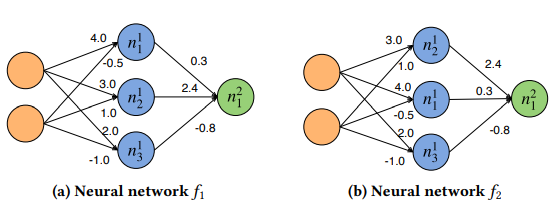
\includegraphics[width=12cm]{figures/permutation_invariance}
    \caption{Permutation eines Neuronalen Netzes \cite{P-11}}
    \label{fig:permutation_invariance}
\end{figure} 

Die Methode von Ateniese et al. \cite{P-80} ist auf diverse Machine Learning Modelle wie Hidden Markov Modelle oder Support Vektor Maschinen ausgelegt, weshalb diese bei Neuronalen Netzen nicht sonderlich gut funktioniert. 
Ganju et al. \cite{P-11} passten den Angriff auf Neuronale Netze an, indem zwei geeignete Repräsentation für diese Art von Modellen genutzt werden kann.
Die erste Repräsentation eines Neuronalen Netz basiert auf der Eigenschaft von Neuronalen Netzen, dass die Reihenfolge der Neuronen vertauscht werden kann. 
Abbildung \ref{fig:permutation_invariance} zeigt zwei Neuronale Netze, bei denen die Reihenfolge der Knoten in der ersten Hidden Layer vertauscht ist, jedoch das Modell die gleiche Funktion berechnet.
Diese Eigenschaft kann nun genutzt werden, um jede Schicht zu sortieren und dadurch eine einheitliche Matrix für Permutationen des gleichen Modells zu erhalten.

Die zweite Repräsentation beruht darauf, die Schichten eines Neuronalen Netzes nicht als Vektor darzustellen.
Im Gegensatz zu einem Vektor hat ein Set keine feste Reihenfolge oder Ordnung, sondern ist lediglich eine Menge von Objekten, bzw. hier von Knoten.
Dies sorgt ebenfalls dafür, dass Permutationen des gleichen Modells, in das gleiche Format übertragen werden können.
Ganju et al. \cite{P-11} zeigen anhand des MNIST Datensatzes, dass beide Repräsentationsformen die Accuracy des Meta-Klassifikators erhöhen können.

Gopinath et al. \cite{P-12} zeigen, dass viele Informationen eines Neuronalen Netzes in der Aktivierung der Neuronen steckt. 
Dabei reicht es, einen Wert in \textbf{on} und \textbf{off} zu unterteilen, wobei on einem Wert > 0 entspricht. 
Gopinath et al. \cite{P-12} nutzten diese Darstellung für eine gutwillige Informationsgewinnung über ein Modell, jedoch könnte die Darstellung auch für Property Inference Angriffe genutzt werden.
\section{Model Inversion Attacke}\label{sec:model_inversion}

Bei der Model Inversion Attacke, versucht ein Angreifer, durch bestimmte Eingaben in ein Modell, Rückschlüsse auf die Trainingsdaten von diesem zu ziehen. 
Dies kann so weit führen, dass einzelne Datensätze nachgebildet werden können \cite{P-3}. 

Fredrikson \etal \cite{P-3} zeigen anhand eines Gesichtserkennungsmodells, dass es möglich ist, das Bild einer Person zu rekonstruieren.
Dabei handelt es sich um einen sogenannten White-Box Angriff.
White-Box bedeutet, dass das Modell vollumfänglich in den Händen des Angreifers ist.
Dies ist beispielsweise der Fall, wenn ein Modell öffentlich geteilt wird.
Eine weitere Voraussetzung ist, dass die zu rekonstruierende Person von dem anzugreifenden Modell klassifiziert werden kann, folglich auch Bilder dieser Person in den Trainingsdaten vorhanden sind.
Abbildung \ref{fig:mi_attacke} zeigt, wie sehr das rekonstruierte Bild (links) dem Originalbild (rechts) ähnelt.

\begin{figure}[!htb]
    \centering
    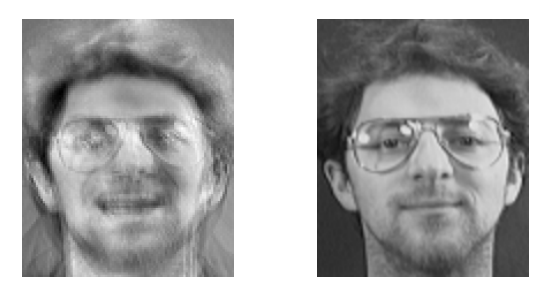
\includegraphics[width=8cm]{figures/mi_attack}
    \caption{Rekonstruktion eines Bildes \cite{P-3}}
    \label{fig:mi_attacke}
\end{figure} 

Der Angriff, auch Reconstruction Attacke genannt, wird durch einen iterativen Algorithmus durchgeführt.
Zu Beginn wird ein initiales Bild, als Startbild gesetzt. 
Hat der Angreifer Hintergrundwissen zu den Daten, so kann er das initiale Bild ähnlich zu dem Zielbild setzen, ansonsten kann es mit festgelegten konstanten Werten oder zufälligen Werten initialisiert werden. 
In jedem Schritt des Algorithmus wird dieses Bild durch das Modell inferiert und anschließend der Wert einer Verlustfunktion bestimmt.
Der Wert dieser ist, sofern das Modell nicht mehr Details zur Vorhersage angibt, lediglich der Wert 1 minus die Wahrscheinlichkeit, auch Confidence Score genannt, ob es sich bei dem eingegebenen Bild um die gesuchte Klasse, auch Label genannt, handelt.
Konkret bedeutet dies, wenn das Bild bereits die zu rekonstruierende Person zeigt, ist der Confidence Score des Labels der Person nahe 1 und damit der Wert der Verlustfunktion nahe 0.
Der Wert der Verlustfunktion kann nun durch das Modell abgeleitet werden und ergibt somit Gradienten für das Bild.
Dies gleicht dem Backpropagation Schritt des Trainings eines neuronalen Netzes, mit dem Unterschied, dass hier das Bild wie ein Teil des Modells behandelt wird und für dieses ebenfalls Gradienten berechnet werden.
Diese Gradienten werden genutzt, um das Bild entgegengesetzt dieser Gradienten anzupassen, sodass der Wert der Verlustfunktion sinkt.
Zusätzlich nutzen die Autoren einen Autoencoder, welcher das angepasste Bild in jedem Schritt harmonisiert und hochskaliert.
Bei diesem Autoencoder handelt es sich um ein neuronales Netz, welches einen Input (hier ein Bild) in einen Vektor mit niedrigerem Rang transformiert und anschließend wieder in einen Vektor mit dem gleichen Rang wie der des Inputs transformiert.
Input und Output eines Autoencoders haben somit den gleichen Rang, hier wird also ein Bild zu einem anderen Bild der gleichen Größe transformiert.
Der Teil des Autoencoders, welcher das Eingabebild in einen Vektor mit niedrigerem Rang transformiert, wird Encoder genannt. 
Der Teil des Autoencoders, welcher das Hochskalieren übernimmt, heißt Decoder.
Zum Training des Autoencoders werden Bilder genutzt, wobei der Input auch gleich dem gewünschten Output entspricht. 
Somit lernt ein Autoencoder, aus einem Bild das gleiche Bild zu erzeugen, jedoch mit der Einschränkung, dass der Vektor innerhalb des Modells einen niedrigen Rang hat.
Folglich ist das erzeugte Bild nicht exakt identisch zu dem eingegebenen Bild.
Der Autoencoder von Fredrikson \etal \cite{P-3} weist jedoch die Besonderheit auf, dass die Eingabebilder verrauscht werden und die gewünschten Ausgabebilder gleich bleiben.
Ziel dadurch ist es, dass der trainierte Autoencoder genutzt werden kann, um unscharfe Bilder zu möglichst scharfen Bildern zu transformieren.
Mit diesem Autoencoder soll also das rekonstruierte Bild nach jeder Iteration schärfer werden und damit näher an dem ursprünglichen Bild liegen.
Die Reconstruction Attacke läuft so lange, bis die maximal konfigurierte Anzahl an Schritten erreicht wird, der Wert der Verlustfunktion einen bestimmten Wert unterschreitet oder sich eine definierte Anzahl an Schritten der Wert der Verlustfunktion nicht reduziert.

Zhang \etal \cite{P-4} erweitern diesen Angriff, indem die Qualität des Autoencoders verbessert wird. 
Der Autoencoder wird nicht nur auf verschwommenen Bildern trainiert, sondern zusätzlich noch auf Bilder, bei welchen jeweils nur ein Bildausschnitt maskiert wird.
Eine weitere Verbesserung besteht darin, zusätzlich ein Modell zu nutzen, welches reale Bilder von synthetischen Bildern unterscheiden soll.
Dieses Konstrukt entspricht dem Diskriminator eines Generative Adversarial Networks \cite{P-86}.
Als Input nutzt dieser Diskriminator Bilder, welche von dem Autoencoder generiert wurden.
Der Wert einer Verlustfunktion des Outputs des Diskriminators kann dabei nicht nur durch den Diskriminator selbst backpropagiert werden, sondern zusätzlich auch noch durch den Autoencoder.
Dies sorgt dafür, dass der Autoencoder ergänzend versucht, möglichst realistische Bilder zu erzeugen.
Mithilfe der zusätzlichen Trainingsdaten und des Diskriminators, wird der Autoencoder verbessert, wodurch die Qualität der einzelnen Bilder erhöht wird und folglich auch die Qualität des rekonstruierten Bildes steigt.
Der restliche Angriff erfolgt simultan zu der bereits beschriebenen Vorgehensweise.
Zhang \etal \cite{P-4} zeigen einen zusätzlichen Angriffsvektor, bei dem ein Angreifer bereits Teile eines Bildes hat. 
Dabei kann es sich um eine verschwommene Version des originalen Bildes handeln, oder um ein Bild, bei dem ein Teil beispielsweise mit einem schwarzen Balken zensiert wird.
Da der Autoencoder zusätzlich mit diesen Fällen trainiert wurde, ist es möglich, die fehlenden Informationen eines Bildes zu ergänzen.



\section{Membership Inference Angriff}\label{sec:membership_inference}

Bei der Membership Inference Attacke versucht ein Angreifer herauszufinden, ob ein Datenpunkt Bestandteil des Trainingsdatensatzes eines Modells ist. 
Dies bedroht die Vertraulichkeit, da beispielsweise herausgefunden werden kann, ob eine bestimmte Person Teil eines Trainingsdatensatzes für die Diagnose einer Krankheit ist und folglich auch mit der entsprechenden Krankheit diagnostiziert ist \cite{P-2}.

Shorki et al. \cite{P-2} führen eine Membership Inference Attacke durch, indem eine Reihe Modelle trainiert wird, die ähnlich dem Angriffsziel-Modell sind.
Diese Modelle werden auch Shadow Modelle genannt.
Ähnlich bedeutet hier, dass sowohl die Funktion der Modelle, als auch der Trainingsdatensatz, mit dem angegriffenen Modell vergleichbar sind.
Einige dieser trainierten Modelle enthalten den zu untersuchenden Datenpunkt im Trainingsdatensatz, andere hingegen nicht.
Nun wird ein binärer Meta-Klassifikator trainiert (analog zu der Property Inference Attacke in Kapitel \ref{sec:property_inference}), welcher anhand der Vorhersagen der Shadow Modelle, Label und Confidence Score, lernt, ob ein Datensatz im Training des entsprechenden Modells genutzt wurde.
Wird in diesen Meta-Klassifikator die Vorhersage des angegriffenen Modells als Input genutzt, so erhält man die Antwort, ob der Datenpunkt für das Modelltraining genutzt wurde oder nicht.
Laut Shorki et al. \cite{P-2} funktioniert dieser Angriff, da ähnliche Modelle, die mit einem ähnlichen Datensatz trainiert wurden, sich auch ähnlich verhalten. 
Somit kann bei den selbst trainierten Modellen, welche den Datensatz enthalten, ein Muster gelernt werden, welches auch auf andere Modelle anwendbar ist. 
Overfitting und eine komplexe Modellarchitektur erhöhen die Wahrscheinlichkeit eines erfolgreichen Angriffs.

Carlini et al. \cite{P-13} zeigen eine Alternative des Angriffs, bei welcher kein Meta-Klassifikator genutzt wurde.
Die Shadow Modelle werden analog zu \cite{P-2} trainiert. 
Anstatt mit den Vorhersagen dieser Modelle nun einen Meta-Klassifikator zu trainieren, werden zwei Gaußverteilungen gebildet, jeweils über die Confidence Scores der Modelle, wo der Datenpunkt im Training enthalten war oder nicht.
Mittels eines Likelihood-Quotienten-Tests wird anschließend vorhergesagt, in welcher Verteilung der Confidence Score des angegriffenen Modells wahrscheinlicher liegt.
Ein Vorteil dieser Methode liegt darin, dass weniger Shadow Modelle trainiert werden müssen, da bereits mit relativ wenig Werten eine Gaußverteilung modelliert werden kann.


Eine Voraussetzung bei Shorki et al. \cite{P-2} ist es, dass der Confidence Score mit ausgegeben wird.
Choquette-Choo et al. \cite{P-7} wandeln den Angriff ab, sodass dieser Score nicht mehr benötigt wird.
Der Angriff funktioniert simultan zu \cite{P-2}, jedoch wird nicht nur der Datenpunkt selber in die Modelle als Input gegeben, sondern auch Abwandlung davon. 
Diese Abwandlungen könnte das Hinzufügen von zufälligem Rauschen sein, oder bei Bilddateien beispielsweise Rotation oder Translation.
Die Hypothese der Autoren ist, dass das Modell bei Datenpunkten, die im Training genutzt wurden, robuster gegenüber diesen Abwandlungen ist und dennoch den Datenpunkt korrekt klassifiziert.
Zusätzlich könnten Abwandlungen der Daten über einen Data Augmentation Schritt auch direkt vom Modell gelernt worden sein.


\section{Data Extraction Attacke}\label{sec:data_ext}

Bei der Data Extraction Attacke versucht ein Angreifer, Informationen eines Modells zu extrahieren, die gelernt wurden, obwohl dies (oftmals) nicht der Fall sein sollte \cite{P-87}.
Der Angriff unterscheidet sich von der Model Inversion Attacke (Kapitel \ref{sec:model_inversion}) und von der Property Inference Attacke (Kapitel \ref{sec:property_inference}), indem Daten direkt aus dem Modell extrahiert werden und nicht anhand der Vorhersage des Modells nachgebildet werden.

Carlini et al. \cite{P-87} beschrieben, dass konkrete Zeichenketten oder Werte, wie eine Kreditkartennummer oder eine Sozialversicherungsnummer, in einem Sprachmodell gelernt werden.
Um dies zu evaluieren, wurde ein Sprachmodell mit dem Penn Treebank Datensatz trainiert, welcher ca. 5MB groß ist. 
Zusätzlich wurde ein Satz eingefügt, welcher mit \textit{\dq My social security number is \dq} beginnt und anschließend eine Zahlenfolge beinhaltet.
Die Funktionalität des Modells liegt darin, das nächste Wort oder Zeichen vorherzusagen, wenn eine Zeichenkette eingegeben wird.
Anzumerken ist hierbei noch, dass dieses Modell signifikant kleiner als 5 MB ist, was folglich bedeutet, dass nicht alle Trainingsdaten in dem Modell gespeichert sein können.
Die Experimente von Carlini et al. \cite{P-87} zeigen, dass dieses Modell die Zahlenfolge ungewollt gelernt hatte als mögliche Vorhersage ausgibt, wenn der oben genannte Satz als Input genutzt wird.

In einem anderen Forschungsprojekt, ebenfalls unter der Leitung von Carlini, \cite{P-88} zeigen die Autoren eine Data Extraction Attacke am Beispiel des Sprachmodells GPT-2. 
Dabei handelt es sich um ein Sprachmodell des Unternehmens OpenAI, welches der Vorgänger von ChatGPT (siehe Kapitel \ref{sec:introduction}) ist und Open Source zur Verfügung steht.
Obwohl voller Zugriff auf das Modell besteht, wird lediglich die Ausgabe des Modells betrachtet. 
Folglich bedeutet dies, dass der Angriff auf jedes Modell anwendbar wäre.
Zur Durchführung des Angriffs wird lediglich ein Starttoken in das Modell eingegeben und anschließend vielfach das vorgeschlagene Folgewort gesammelt. 
Wird dies lang genug gemacht, erhält man eine lange Tokenabfolgen, also quasi Sätze, die vom Modell gelernt wurden. 
Dabei kann es sich um öffentliche Texte handeln, wie beispielsweise der Text der MIT Open Source Lizenz, aber auch private Daten wie Email-Adressen sind vorhanden.
Diese Variation des Angriffs kann in gewissem Maße funktionieren, liefert jedoch oftmals gleiche Wortabfolgen und hat auch eine hohe False-Positive Rate.
Carlini et al. \cite{P-88} variierten deshalb die Methodik, wie die Tokenabfolge gesammelt wird.
Bevor GPT-2 das wahrscheinlichste Folgewort vorschlägt, werden die Wahrscheinlichkeiten in den Wertebereich (0,1) transformiert und so skaliert, dass diese Werte addiert 1 ergeben.
Wird der Softmax Funktion ein Hyperparameter namens Temperatur > 1 mitgegeben, wird das Modell unsicherer und erhöht dadurch die Diversität der Vorhersagen des Modells.
Neben dieser Temperatur wird eine zweite Verbesserung vorgeschlagen. 
Anstatt nur einen Starttoken zu nutzen, werden die ersten Wörter von verschiedenen, öffentlichen Datenquellen genutzt.
Mit diesen zwei Verbesserungen konnten mehr unterschiedliche Arten von Texten, die das Modell gelernt hat, extrahiert werden. 
Neben Newsartikeln oder Forumsbeiträgen, befanden sich auch Kontaktdaten einiger Privatpersonen in diesen Tokenabfolgen.
\section{Poisoning Attacke}\label{sec:poisoning}

Bei der sogenannten Poisoning Attacke werden manipulierte Datensätze in die Trainingsdatenmenge eines Modells injiziert, wodurch das Modell schlechtere oder sogar falsche Vorhersagen trifft.
Ursprünglich ist diese Art des Angriffs recht populär bei Support Vektor Maschinen.
Biggio \etal \cite{P-15} zeigen, dass einige modifizierte Datenpunkte in der Nähe der Entscheidungsgrenze einer Support Vektor Maschine genügen, um die gelernte Funktion deutlich negativ zu beeinflussen.

Yang \etal \cite{P-17} zeigen ein Verfahren, bei dem eine Poisoning Attacke auf neuronalen Netzen angewendet wird.
Ziel hierbei ist es, die gefälschte Daten mit einem absichtlich falschen Label so zu wählen, dass der Wert der Verlustfunktion möglichst groß ist. 
Um dies zu erreichen, wird der Wert der Verlustfunktion des anzugreifenden Modells durch das Modell backpropagiert, wobei die gefälschten Daten als Teil des Modells betrachtet werden. 
Die Daten werden nun in Richtung der Gradienten angepasst, wodurch der Wert der Verlustfunktion steigt.
Werden die gefälschten Daten anschließend genutzt, um das Modell weiter zu trainieren, wird die Verlustfunktionen einen erhöhten Wert aufweisen, was zu einer stärkeren Anpassung des Modells führt, was aufgrund der gefälschten Label zu einer Verschlechterung der Güte des Modells führt.
Um nicht als gefälschte Daten aufzufallen, nutzen Yang \etal \cite{P-17} einen Autoencoder, der Daten so transformiert, dass diese vom Modell als echte Daten erkannt werden.
Damit der Autoencoder lernt, realistische Daten nachzubilden, wird ein zusätzliches Modell genutzt, welches einem Diskriminator der Generative Adversarial Network Architektur \cite{P-86} entspricht.

Guo und Liu \cite{P-16} nutzen einen Ansatz, bei welchem der Angreifer keinen Zugriff auf die Gradienten des angegriffenen Modells braucht.
Stattdessen wird ein vortrainiertes Modell genutzt, welches ähnlich zu dem angegriffenen Modell ist. 
Da diverse Modellarchitekturen Open-Source sind, finden sich auch einige vortrainierte Varianten von diesen im Internet.
Bei Bildklassifikation lässt sich beispielsweise ein vortrainiertes YOLO-Modell nutzen.
Dieses kann dann genutzt werden, um ein generatives Modell zu trainieren, welches wie bei Yang \etal \cite{P-17} die Gradienten des anzugreifenden Modells nutzt, um Daten für das anzugreifende Modell zu verschlimmern.
Guo und Liu \cite{P-16} gehen davon aus, dass das angegriffene Modell noch optimiert wurde und deshalb eine bessere Feature-Erkennung hat, als die öffentlich vortrainierten Modelle.
Dies macht den Angriff effektiver, sofern die Modelle nicht zu unterschiedlich sind.

Poisoning Attacken verschlechtern in der Regel lediglich die Performance eines Modells und sorgen für falsche Vorhersagen.
Tramèr \etal \cite{P-14} zeigen jedoch, dass manipulierte Daten dafür sorgen können, dass andere Angriffe, welche die Vertraulichkeit angreifen, effektiver werden können.
Durch Ändern des Labels eines Datensatzes kann dieser gegebenenfalls zu einem Ausreißer transformiert werden. 
Dadurch passt sich das Modell stärker diesem an, als wenn sich der Datenpunkt in die Messreihe einordnet.
Die falsche Klassifizierung des veränderten Datensatzes würde eine Memberhsip Inferenze Attacke auf diesen verbessern.

\subsection{Verteiltes Lernen}\label{sec:verteiltes_lernen}

Das Verteilte Lernen bietet einige besondere Herausforderungen, die bereits in Kapitel \ref{sec:angriffe_verteiltes_lernen} betrachtet wurden. 
Einige bereits beschriebene Methoden lassen sich problemlos auf das Verteilte Lernen anwenden.
Sollen beispielsweise die Daten der einzelnen Teilnehmer geteilt werden, so ist es möglich, diese mit den Methoden aus Kapitel \ref{sec:aufbereitung_datensatz} vorzuverarbeiten.
Jedoch gibt es auch spezielle Methoden, die auf das Verteilte Lernen ausgerichtet sind.
Im Folgenden werden einige davon genauer beschrieben.

\subsubsection*{Distributed Selective SGD}
Shokri und Shmatikov \cite{P-78} stellen eine Methode vor, bei welcher mehrere Teilnehmer gleichzeitig ein Modell trainieren, ohne dabei die Daten untereinander zu teilen.
Diese wird Distributed Selective Stochastic Gradient Descent oder auch Distributed Selective SGD genannt.
Das Modell liegt dabei auf einem zentralen Server.
Bei der ersten Iteration laden die Teilnehmer das gesamte Modell herunter, bei weiteren Iterationen nur eine festgelegte Anzahl der am meisten geupdateten Parametern (Gewichte).
Dadurch soll vermieden werden, dass Overfitting auf den Daten eines einzelnen Teilnehmers auftritt.
Die heruntergeladenen Parameter ersetzen die alten Parameter an der entsprechenden Stelle im lokalen Modell.
Anschließend wird dieses lokale Modell mit den eigenen Daten trainiert und im Nachhinein eine festgelegte Menge an Gradienten übertragen. 
Diese können dabei entweder randomisiert ausgewählt werden, oder möglichst nach Größe sortiert werden.
Alle Teilnehmer wählen die zu teilenden Gradienten mit der gleichen Strategie aus und behalten diese über den Trainingsprozess bei.
Zusätzlich ist es möglich, die Gradienten vor dem Teilen noch mit in der Größe zu begrenzen oder Rauschen mittels Differential Privacy hinzuzufügen.
Abbildung \ref{fig:dssgd} zeigt die Architektur von Distributed Selective SGD.

\begin{figure}[!htb]
    \centering
    \includegraphics[width=12cm]{figures/dssgd}
    \caption{Distributed Selective SGD \cite{P-78}}
    \label{fig:dssgd}
\end{figure} 

Durch das eingeschränkte Teilen der Gradienten werden so wenig Information wie nötig geteilt, jedoch ist die Güte des Modells kaum schlechter als bei normalem Training.
Die Autoren begründen dies damit, dass das lokale Modell lokale Minima durch das Ersetzen von Parametern aus dem geteilten Modell verlassen kann und so weiter eher Richtung globales Minimum konvergiert. 
Zwei Parameter steuern dabei die Performance des Modells beim Training mit Distributed Selective SGD: das Privacy Budget $\epsilon$ und die Anzahl der zu teilenden Gradienten.
Werden mehr Gradienten nach jedem Schritt von jedem Teilnehmer geteilt, kann das Privacy Budget $\epsilon$ niedriger angesetzt werden, um dennoch eine nahezu identische Güte im Vergleich zu einem normal trainierten Modell zu erhalten.

\subsubsection*{Anspruchsvolle kryptografische Methoden}

Takabi et al. \cite{P-104} nutzen Homomorphe Verschlüsselung, um ein Modell zu trainieren, welches Daten von mehreren Teilnehmern nutzen kann. 
Die Funktionsweise der Methode mit einem Teilnehmer wurde bereits in Kapitel \ref{sec:homomorphe_verschlüsselung} beschrieben.
Diese lässt sich problemlos auf mehrere Teilnehmer erweitern, indem abwechselnd Daten jedes Teilnehmers verschlüsselt an den Server übertragen wird und diese für das Training des Modells mittels Homomorpher Verschlüsselung genutzt wird.
Da Daten jeweils verschlüsselt sind, ist es nicht möglich, Daten anderer Teilnehmer zu extrahieren.

Auch das auf Funktionaler Verschlüsselung basierende Framework CryptoNN \cite{P-53}, welches in Kapitel \ref{sec:funktionale_verschlüsselung} vorgestellt wurde, kann für Verteiltes Lernen genutzt werden. 
Die Rolle des Clients können dabei mehrere Teilnehmer übernehmen, wohingegen die Autorität jedoch von einem separaten System übernommen werden muss. 
Anschließend können auch bei dieser Methode abwechselnd Daten von verschiedenen Teilnehmern zum Trainieren genutzt werden.

Ein weiterer Ansatz für Verteiltes Lernen, welches auf Funktionaler Verschlüsselung basiert, wurde von Xu et al. \cite{P-33} mit dem Namen HybridAlpha vorgestellt.
Ähnlich zu dem bereits beschriebenen CryptoNN Framework, gibt es auch eine Autorität, welche die benötigten kryptografischen Schlüssel an die Server und Clients verteilt.
Jedoch übertragen die Clients keine Daten an den Server, sondern trainieren ein lokales Modell.
Die aktualisierten Modellparameter werden anschließend mit Differential Privacy verrauscht und dann verschlüsselt an den Server übertragen.
Hat der Server alle verschlüsselten Modellparameter jedes Teilnehmers gesammelt, wird mittels Funktionaler Verschlüsselung die Summe der Gewichte jedes Neurons gebildet.
Daraus kann der Server anhand der Anzahl an Teilnehmern, den Durchschnittswert für jedes Gewicht jedes Neurons bilden und aktualisiert damit das globale Modell.
Die Autoren zeigen anhand des MNIST Datensatze \cite{D-MNIST}, dass die Güte eines Modells, welches mit HyrbidAlpha ohne Differential Privacy trainiert wurde, sehr nahe der Güte eines Modells ist, welches in einem Verteilten Lernen Szenario ohne HyrbidAlpha gelernt wurde. 
Wird jedoch zusätzlich Differential Privacy genutzt, sinkt die Güte des Modells. 
Mit einem Privacy Budget von $\epsilon=0,5$ sinkt die Genauigkeit der Klassifikation um knapp 10\%.


\subsubsection*{Secure Multi-Party Computation}

Bei der Secure Multi-Party Computation handelt es sich um einen Forschungsbereich mit dem Ziel, dass Teilnehmer gemeinsam eine Funktion berechnen können, ohne dass die einzelnen Eingabewerte aufgedeckt werden. 
Methoden dieses kryptografischen Forschungsgebiets können auch für Neuronale Netze genutzt werden.

Rouhani et al. \cite{P-71} stellten ein Framework namens DeepSecure vor, welches Oblivious Transfer, zu Deutsch vergessliche Übertragung, und Garbled Circuits, zu Deutsch verdrehte Schaltkreise, nutzt.
Oblivious Transfer ist ein kryptografisches Protokoll zwischen einem Sender und einem Empfänger, bei dem der Empfänger einen Index zwischen 1 und $n$ auswählt und der Sender die Nachricht mit dem entsprechenden Index übermittelt. 
Der Sender weiß dabei jedoch nicht, welcher Index ausgewählt wurde.
Diese Methodik wird auch 1-aus-$n$ Oblivious Transfer genannt.
Garbled Circuits, auch Yao's Garbled Circuits genannt, ist ebenfalls ein Protokoll, bei der eine Funktion als Boolescher Schaltkreis mit zwei Eingabegattern dargestellt wird.
Dabei erstellt einer der beiden Teilnehmer, hier Alice genannt, Wahrheitstabellen zu jedem Logikgatter des Schaltkreises. 
Die Inputs sind dabei nicht 0 und 1, sondern jeweils eine Folge von $k$ randomisierten Bits, welche 0 und 1 kodieren.
Die Ergebnisspalte dieser Wahrheitstabellen verschlüsselt Alice anschließend mit den beiden Inputs, sodass dies nur mit den beiden Inputs wieder entschlüsselt werden kann. 
Zusätzlich wird die Reihenfolge der Zeilen randomisiert, damit aufgrund der Reihenfolge keine Rückschlüsse gewonnen werden können. 
Dieser Schritt wird Garbling genannt und die entstandenen Tabellen sind sogenannte Garbled Tabellen.
Anschließend überträgt Alice die Garbled Tabellen an den zweiten Teilnehmer, hier Bob.
Mittels 1-aus-2 Oblivious Transfer wählt Bob eine von zwei Nachrichten aus, wobei der Index seinem Input entspricht und die zwei Nachrichten die kodierten Labels von Alice sind.
Die erhaltene Nachricht und das eigene Label können nun genutzt werden, um die Ergebnisspalte einer Garbled Tabelle zu entschlüsseln.
Bob führt dies für jedes Gatter des Schaltkreises aus.
Am Ende erhält Bob den Output des letzten Gatters, welchen jedoch einer der randomisierten Bitfolgen ist. 
Er übermittelt diesen an Alice und erhält dadurch den entsprechenden 0 oder 1 Wert.
DeepSecure wendet Garbled Circuits auf Neuronale Netze an.
Alice würde in diesem Fall die Daten besitzen und Bob das Modell, welches trainiert wird.
Der Feedforward Schritt würde dabei durch einen Booleschen Schaltkreis aus XOR und XNOR Gattern implementiert werden, wodurch die Berechnung der Vorhersage erfolgt.
Dadurch kann Bob den Wert der Verlustfunktion und anschließend der Gradienten bestimmen, ohne die Daten von Alice zu kennen.
Alice würde jedoch auch nicht die genauen Gewichte des Modells kennen.
Allerdings ist die Anzahl an benötigten Gattern, um ein Neuronales Netz darzustellen, enorm.
Einige Operationen, wie die Anwendung einer Aktivierungsfunktion, benötigt mehrere tausende Gatter.
Jedes dieser Gatter sorgt ebenfalls dafür, dass eine Menge an Daten übertragen werden muss.
Ein Neuronales Netz, welches $28\times28$ Pixel Bilder als Input nimmt, zwei Hidden Layers mit 300 und 100 Knoten (Sigmoid Aktivierungsfunktion) besitzt und eine Softmax Output Layer mit 10 Knoten hat, würde circa 171.300.000 Gatter ausmachen und in einem Feedforward Schritt ungefähr 2 Gigabyte an Daten übertragen.

\subsubsection*{Aggregation}
Eine alternative Methode wird von Bonawitz et al. \cite{P-36} vorgestellt.
Diese basiert auf sicherer Aggregation, welche mehrere Daten von unterschiedlichen Teilnehmern verbindet, ohne dass die Daten eines einzelnen Teilnehmers erkenntlich werden.
Teilnehmer trainieren ein lokales Modell mit den eigenen privaten Daten. 
Bevor die angepassten Parameter aber an das globale Modell übertragen werden, werden die Parameter mit den Parametern anderer Teilnehmer kryptografisch aggregiert.
Dadurch erhält das globale Modell Gradienten aller Trainingsdaten, ohne die einzelnen Daten zu kennen.


%\section{Weitere Angriffe}

Neben den bereits beschriebenen Angriffe, gibt es noch einige zusätzliche Angriffe, wo jedoch nicht die Vertraulichkeit der Daten im Visier des Angreifers liegt. 
Für die Vollständigkeit dieses Kapitels, werden einige relevante Angriffe dennoch erwähnt.
Weiterentwicklungen oder Abwandlungen könnten in Zukunft dennoch Einfluss auf die Vertraulichkeit der Daten haben, so wie es bereits bei der Poisoning Attacke in Kapitel \ref{sec:poisoning} beschrieben wurde.

\subsection{Evasion Attack}



\subsection{Backdoor Attack}
\chapter{Methoden zur Sicherung der Vertraulichkeit}\label{sec:methoden}

Neben den beschriebenen Angriffen aus Kapitel \ref{sec:angriffe} gibt es eine Vielzahl an Methoden, diese abzuschwächen oder sogar ganz zu unterbinden.
Dieses Kapitel stellt zuerst eine typische Pipeline zum Training eines Neuronalen Netzes vor und teilt diese in 3 Phasen ein.
Phase 1 ist dabei die Aufbereitung des Datensatzes, also jegliche Verarbeitung der Daten, die vor dem eigentlichen Training stattfinden.
Anschließend folgt Phase 2, welche das Training des Modells umfasst.
Das Ende der Pipeline, Phase 3, beinhaltet das Deployment so wie den Betrieb des Modells.
Die Gegenmaßnahmen werden jeweils der entsprechenden Phase untergeordnet.

\section{Übersicht der Pipeline}


Abbildung \ref{fig:ml_pipeline} zeigt den Aufbau der typischen Pipeline, um ein Neuronales Netz zu trainieren. 
Diese wird im Folgenden genauer beschrieben.
Schritt 1 ist die Vorverarbeitung der Daten.
Die Daten können dabei aus einer Datenbank oder einem Filesystem stammen, die im Voraus gesammelt wurden.
Die Vorverarbeitung der Daten ist recht individuell und kann je nach Anwendungsfall variieren. 
Typische Handlungen sind:
\begin{compactitem}
\item Vereinheitlichung des Datenformats
\item Fehler und starke Ausreißer werden entfernt
\item Normalisierung der Daten
\item Erstellung neuer Daten durch Transformationen
\item Kodierung von (kategorialen) Variablen und Labels
\item Aufteilung in Trainings-, Validierungs- und Testdatensätze
\end{compactitem}
\begin{figure}[!htb]
    \centering
    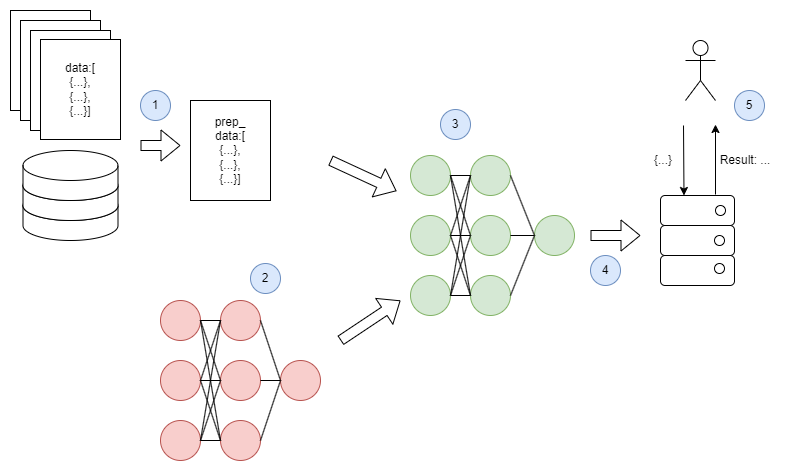
\includegraphics[width=14cm]{figures/ml_pipeline.png}
    \caption{Training eines Neuronalen Netzes}
    \label{fig:ml_pipeline}
\end{figure} 

Die Abbildung \ref{fig:ml_pipeline} stellt die Vorverarbeitung in einem Schritt dar, bei dem mehrere Datenquellen verbunden werden und nur ein Dokument übrig bleibt. 
Dieses eine Dokument soll zeigen, dass nur die wichtigen Informationen der Daten erhalten bleiben, jedoch kann es in der Praxis sein, dass die Datenmenge beim Aufbereiten der Daten größer wird. 
Kapitel \ref{sec:training_modells} stellt verschiedene Methoden vor, die bei der Vorverarbeitung der Daten angewendet werden können, um die Vertraulichkeit zu sichern.

Schritt 2 umfasst die Architektur eines Modells.
Je nach Anwendungsfall und Komplexität der Aufgabe, werden unterschiedliche Konfigurationen der einzelnen Schichten vorgenommen.
Dabei werden die Gewichte zufällig oder anhand einer Verteilung initialisiert.
In der Abbildung wird dies durch ein rotes Modell angezeigt, da Gewichte des Modell zufällig (oder anhand einer Verteilung) initialisiert sind, und noch keine sinnvolle Vorhersage getroffen werden kann.
Schritt 3 ist der tatsächliche Trainingsvorgang, bei dem das untrainierte Modell lernt.
Grob lässt sich das Training in folgende Schritte einteilen, die mehrfach mit jedem Datenpunkt durchgeführt werden können:
\begin{compactenum}
\item Ein Datenpunkt oder ein mehrere Datenpunkte (Batch) werden durch das Modell gegeben und die Vorhersage berechnet. Die Abweichung von der tatsächlichen Vorhersage zu dem Label des Datenpunktes wird mittels einer Verlustfunktion quantifiziert.
\item Mittels des Wertes der Verlustfunktion lassen sich Gradienten für die Gewichte des Neuronalen Netzes berechnen. Diese können dazu genutzt werden, die aktuellen Gewichte anzupassen. Dieser Schritt wird Backpropagation genannt.
\end{compactenum}
Ein Durchgang der obigen Schritte mit jedem Datenpunkt wird dabei Epoche genannt. 
Um den Trainingsfortschritt zu beobachten, kann eine Epoche zusätzlich auch eine Evaluierung mittels eines Validierungsdatensatzes enthalten.
Grafisch wird das Training durch den Verbund des Dokuments und des untrainierten, roten Modells dargestellt. 
Es entsteht ein grünes Modell, welches in der Lage ist, sinnvolle Vorhersagen zu erzeugen.
In der Praxis gibt es hier einige Iterationen des Training, welche zusätzliche Vorgänge, wie beispielsweise eine Validierung, enthalten. 
Kapitel \ref{sec:training_modells} widmet sich Methoden, die während des Trainings, welche aus Schritt 2 und 3 besteht, angewendet werden.

Schritt 4 und 5 beschreiben das Deployment und den Betrieb des Modells. 
Dieses soll für vorgesehene Anwender erreichbar sein. 
Je nach Anwendungsfall kann die Systemarchitektur unterschiedlich aussehen. 
Einige Modelle werden mit Trainingscode auf öffentlichen Plattformen, wie HuggingFace\footnote{https://huggingface.co/models}, geteilt, wohingegen andere Modelle, wie ChatGPT\footnote{https://chat.openai.com/}, nur über eine spezielle Oberfläche erreichbar sind.
In Abbildung \ref{fig:ml_pipeline} zeigt deshalb lediglich einen Anwender, der direkt Request an das Modell schickt.
In Kapitel \ref{sec:betrieb} werden Maßnahmen besprochen, die in dieser Phase die Vertraulichkeit sichern. 
Dabei kann es sich um Transformationen des Modells vor dem Deployment handeln, oder um Mechanismen, die Anfragen und Antworten des Modells abwandeln.
\section{Aufbereitung des Datensatzes}\label{sec:aufbereitung_datensatz}

Bereits beim ersten Schritt einer Machine Learning Pipeline, dem Vorverarbeiten der Daten, können diverse Methoden genutzt werden, um die Vertraulichkeit zu wahren.
In diesem Kapitel werden 3 Kategorien dieser Methoden vorgestellt, und wie diese genutzt werden können, um bereits vor dem eigentlichen Training Modelle sicherer zu machen.

%\subsection{Elimination}
\subsection{Anonymisierung}\label{sec:anonymisierung}

Bei der Anonymisierung von Daten geht es darum, identifizierende Eigenschaften zu entfernen oder unkenntbar zu machen.
Dabei soll dennoch ein gewisser Nutzen erhalten bleiben. 

Sweeney \cite{P-23} stellt eine Methode der Anonymisierung namens \textit{k}-Anonymität (im Englischen \textit{k}-Anonymity) vor.
Die Methode wird im folgenden mittels eines Auszugs des Titanic Datensatzes \cite{D-titanic} erläutert.
Tabelle \ref{tab:nicht_ano_titanic} zeigt einen Auszug aus diesem Datensatz.
Die hier ausgewählten Spalten enthalten beschreibende Merkmale einer Person, sowie Informationen über die Reise auf der Titanic. 
Zur Verdeutlichung gehen wir davon aus, dass es sich bei dem Einstiegsort um eine private Information handelt, die den Wohnort verraten könnte.

\input{tables/nicht_ano_titanic}

Bei \textit{k}-Anonymität werden die Attribute in 3 separate Klassen eingeteilt: Identifikatoren, Quasi-Identifikatoren und sensible Attribute.
Bei diesem Beispiel wäre der Name der einzige Identifikator, da über diesen eine Person eindeutig zugeordnet werden kann. 
Quasi-Identifikatoren sind alle Variablen, welche Information über einen Datenpunkt preisgeben, aber nicht direkt auf diesen schließen lassen. 
Um mit Quasi-Identifikatoren einen Datenpunkt zu identifizieren, braucht es in der Regel mehr Informationen, beispielsweise einen Datensatz.
In diesem Beispiel könnte also jede Spalte ein Quasi-Identifikator sein.
Da der Name bereits ein direkter Identifikator ist, wird dieser anders zugeordnet.
Die dritte Klasse sind die sensiblen Attribute, die es zu sichern gilt. 
Hier gehen wir davon aus, dass der Einstiegsort eine schützenswerte Information ist.
Um \textit{k}-Anonymität zu erreichen, muss jede Kombination aus Quasi-Identifikatoren mindestens k mal vorkommen, wobei k festgelegt werden kann. 
Ein größeres k sorgt für mehr Privatsphäre.
Um dies zu erreichen, können die Quasi-Identifikatoren gruppiert werden, so kann beispielsweise anstatt des Alters, eine Zahlenbereich als Alter dienen.
Tabelle \ref{tab:k-ano-titanic} zeigt wie diese Gruppierung aussieht.

\input{tables/k_ano_titanic}

Es ist zu sehen, dass die Identifikatoren, hier nur der Name, entfernt wurden.
Geschlecht und Buchungsklasse sind auch unverändert geblieben.
Die Gruppierung erfolgte anhand der Quasi-Identifikatoren, wobei das Alter durch einen Zahlenbereich ersetzt wurde.
Hier ist anzumerken, dass die Spanne der Altersgruppen unterschiedlich groß ist. 
Je nachdem wie diese Spannen aufgebaut sind, würden sich die Gruppierungen verändern.
\textit{k}-Anonymität mit k = 2 ist hier erfüllt, da jede Kombination von Quasi-Identifikatoren mindestens 2 mal vorkommt.
Dabei ist es auch möglich, dass einzelne Einträge redundant vorkommen. 
So sind in Tabelle \ref{tab:k-ano-titanic} die ersten beiden Einträge identisch, obwohl diese von 2 unterschiedlichen Personen stammen.

Machanavajjhala et al. \cite{P-24} zeigen anhand von 2 Attacken, dass \textit{k}-Anonymität nicht ausreichend ist.
Bei der Homogenitätsattacke kann die Eigenschaft, dass sensible Attribute nicht einzigartig sind, ausgenutzt werden.
Tabelle \ref{tab:homo_k_ano} zeigt abgewandelt die ersten Zeilen der Tabelle \ref{tab:k-ano-titanic}.
Das sensible Attribut, der Einstiegsort, ist jedoch in dieser Quasi-Identifikatoren Kombination identisch.
Sollte also eine Person männlich, zwischen 20 und 35 Jahren alt sein und in der Buchungsklasse 3 mitgefahren sein, so kennt man auch den Einstiegsort.
\input{tables/homogenitaet_k_ano}

Ein weiteres Problem ist ein Angriff mit Hintergrundwissen, mit dem gewisse sensible Attribute ausgeschlossen werden können oder zumindest unwahrscheinlicher machen könnten.
In diesem Beispiel könnte es also sein, dass ein Angreifer weiß wann, ein Passagier zugestiegen ist und an welchem Hafen das Schiff zu dieser Zeit war. 
Damit können Rückschlüsse auf den Einstiegsort gemacht werden.

Aufgrund dieser beiden Angriffe, schlagen Machanavajjhala et al. \cite{P-24} eine Erweiterung mit dem Namen \textit{l}-Diversität (im Englischen \textit{l}-Diversity) vor.
Dabei wird \textit{k}-Anonymität auf die Daten angewendet und zusätzlich eine Bedingung eingeführt. 
Diese kann sowohl für einen Block, eine einheitliche Kombination der Werte der Quasi-Identifikatoren, als auch für den ganzen Datensatz gelten.
Ein Block ist dabei \textit{l}-divers, wenn die Werte des sensiblen Attributes \textit{\dq gut repräsentiert\dq} sind, wobei l eine Zahl zugeorndet werden kann.
Ist jeder Block des Datensatzes \textit{l}-divers, dann ist auch der ganze Datensatz \textit{l}-divers.
Dabei gibt es 3 Grundvarianten laut Machanavajjhala et al., wie \textit{\dq gut repräsentiert\dq} definiert werden kann \cite{P-24}:
\begin{compactitem}
\item \textbf{Unterscheidbare \textit{l}-Diversität:} Bei dieser Variante, hat ein Block \textit{l} unterschiedliche Werte eines sensiblen Attributes. Ein Block ist daher immer mindestens 1-divers, da dies bedeutet, dass das sensible Attribute immer den gleichen Wert annimmt.
\item \textbf{Entropie \textit{l}-Diversität:} Hier wird die Entropie der sensiblen Attribute eines Blocks berechnet. Dabei ist ein Block \textit{l}-divers, wenn die Entropie $\ge$ log(\textit{l}) ist. Folglich ist 1-Diversität dabei immer gegeben.
\item \textbf{Rekursive (c,\textit{l})-Diversität:} Diese Definition besagt, dass das häufigste sensible Attribut eines Blocks, seltener vorkommt, als die Anzahl der restlichen Attribute, multipliziert mit einem konstanten Wert c. Folglich darf kein sensibles Attribut zu oft vorkommen. Ein Block ist dabei (c, \textit{l})-divers, wenn $\textit{l} - 1$ verschiedene einzigartige Attribute entfernt werden können und die Bedingung immernoch erfüllt ist.
\end{compactitem}

Je nach Datensatz, kann es Sinn ergeben, einige Ausnahmen zu erlauben.
So könnte es sein, dass ein Datensatz von einer Variable dominiert wird, die jedoch keine Verletzung der Privatsphäre darstellt. 
Ein Beispiel der Autoren ist, wenn eine Kardiologie preisgibt, dass die meisten Patienten eine Herzkrankheit haben.
Auf der anderen Seite, gibt es Attribute, die besonders geschützt werden sollten.

Sollte ein Datensatz mehrere sensible Attribute besitzen, so muss \textit{l}-Diversität für jede dieser Attribute gelten. 
Für diese Überprüfung, werden jeweils alle anderen Spalten, auch die sensiblen Attribute, als Quasi-Identifikator angesehen.

Li et al. \cite{P-25} zeigen, dass \textit{l}-Diversität zwei Angriffsflächen bietet.
Die erste Angriffsfläche ergibt sich, wenn die Verteilung des sensiblen Attributs sehr stark links- oder rechtsschief ist.
Die Autoren zeigen ein Beispiel, bei der das sensible Attribut eine Infektion mit einem bestimmten Virus ist.
Dabei sind 99\% der Personen gesund und lediglich 1\% der Personen infiziert. 
Die Verteilung des Attributs ist stark schief. 
Hat jetzt ein Block, der durch \textit{k}-Anonymität entsteht, ein 50\% Aufteilung beider Werte, so wäre dieser Block \textit{l}-divers mit \textit{l} = 2. 
Kann man jedoch eine Person diesem Block zuordnen, so wäre dies ein Informationsgewinn, da besagte Person ein überdurchschnittliches Risiko der Infektion besitzt.
Die zweite Angriffsfläche entsteht dadurch, dass \textit{l}-Diversität nicht berücksichtigt, ob die Werte des Attributes eine ähnliche Bedeutung haben.
Bei einem Krankheitsbeispiel könnten die Werte alle unterschiedliche Krankheiten annehmen, die jedoch das gleiche Körperteil betreffen.
Diese Angriffsfläche ähnelt der Homogenitätsattacke gegen \textit{k}-Anonymität, bloß dass hier zusätzlich Werte semantisch verbunden werden können.

Aufgrund dieser beiden Angriffsflächen stellen Li et al. \cite{P-25} ein neues Maß an Sicherheit vor: \textit{t}-Nähe (im Englischen \textit{t}-Closseness).
Ziel dieses Maßes ist es, zu zeigen, dass die Verteilung eines sensiblen Attributes in einem einzelnen Block ähnlich zu der Verteilung des gleichen Attributes im gesamten Datensatz ist.
Der Unterschied zwischen den beiden Verteilungen soll kleiner als ein Grenzwert \textit{t} sein.
Die Autoren prüfen verschiedene Verfahren der Distanzmessung der Verteilungen und favorisieren die sogenannte Earth Mover Distanz.
Dabei handelt es sich um eine Metrik zweier Verteilungen, welche die minimale Arbeit berechnet, die nötig ist, um eine Verteilung zu der anderen Verteilung zu transformieren, indem Werte innerhalb der Verteilung verschoben werden. 
Die Metrik liegt immer im Wertebereich (0,1) wodurch diese auch vergleichbar ist. 
Ein Wert nahe 0 ist dabei besser.
Mathematisch gesehen, handelt es sich um ein Optimierungsproblem, jedoch gehen die Autoren auf 2 unterschiedliche Arten von Attributen ein, numerische und kategoriale, um zu zeigen, wie die Earth Mover Distanz berechnet wird.
Um die Distanz für numerische Werte berechnet zu werden, müssen diese erstmal sortiert werden. 
Sofern es sich um eine ungleiche Anzahl an Werten handelt, können die Werte mehrfach genutzt werden.
Anschließend wird die durchschnittliche, normalisierte Differenz zwischen den Werten an gleicher Stelle beider sortierten Verteilungen berechnet.
Im Folgenden wird eine Beispielrechnung exerziert, welches ein sensibles Attribut, Stundenlohn in Euro, darstellt. 
Verteilung 1 ist dabei das sortierte Gehalt eines Blockes nach \textit{k}-Anonymität und Verteilung 2 das Gehalt des gesamten Datensatzes:
\begin{addmargin}[25pt]{0pt} Verteilung 1 = \{20, 30, 40\} \\
Verteilung 2 = \{20, 25, 25, 30, 35, 35, 35, 40, 40\} \end{addmargin}
Da Verteilung 2 dreimal so viele Elemente enthält wie Verteilung 1, wird jedes Element dreimal genutzt. 
Dadurch erhält man:
\begin{addmargin}[25pt]{0pt}Verteilung 1' = \{20, 20, 20, 30, 30, 30, 40, 40, 40\} \end{addmargin}
Die größte Differenz ist 40 – 20 = 20, somit wird der Betrag jeder Differenz durch 20 dividiert, dass diese jeweils im Wertebereich (0,1) liegen.
Werden jetzt die einzelnen Wertepaare verglichen, so ergibt sich folgend Distanz:
\begin{addmargin}[25pt]{0pt}
$ (20-20)+(20-25)+(20-25)+(30-30)+(30-35)+(30-35)+(40-35)+\\ (40-35) + (40-40) = -10$
\end{addmargin}
Der durchschnittliche, normalisierte Wert dieser Distanz, ist die gesuchte Earth Mover Distanz:
\begin{addmargin}[25pt]{0pt}
$ 1/9 \times  |-10| \div /20 = 0,056$
\end{addmargin}
Damit hat dieser Block eine 0,056-Nähe, was bedeutet, wenn man einer Person diesem Block zuordnet könnte, ist dennoch kaum Informationsgewinnung möglich.


Bei kategorialen Werten ist es schwieriger, eine Differenz zu bilden.
Es gibt die Möglichkeit den Wert 1 zuzuweisen, wenn die beiden Kategorien unterschiedlich sind und den Wert 0, sofern beide gleich sind. 
Dies würde jedoch bedeuten, dass semantische Ähnlichkeiten der Werte nicht berücksichtigt werden.
Eine Alternative wäre es, alle möglichen Werte semantisch zu in einer Art Baumstruktur zu gliedern. 
Bei Krankheiten wäre beispielsweise die Wurzel \textit{\dq Krankheit\dq}, die Nachfolger wären dann gewisse Systeme des Körpers wie beispielsweise \textit{\dq Herz-Kreislaufsystem\dq} und \textit{\dq Verdauungssystem\dq}.
Die Distanz ist nun die Anzahl der Schritte, die benötigt wird, um die Werte zu verbinden. 
Zwei unterschiedliche Herzkrankheiten sind über einen Schritt mittels \textit{\dq Herz-Kreislaufsystem\dq} verbunden, wohingegen eine Herzkrankheit und eine Darmkrankheit über 2 Schritte mittels der Wurzel \textit{\dq Krankheit\dq} verbunden wären.


%\subsection{Perturbation}
\subsection{Differential Privacy}\label{sec:dp}

Differential Privacy ist eine Technik, welche 2006 von Cynthia Dwork \cite{P-26} vorgestellt wurde.
Ziel dabei ist es, Zugriff auf eine Datenmenge zu ermöglichen, welche sowohl nützliche Erkenntnisse zulässt, als auch die Privatsphäre eines einzelnen Datensatzes schützt.

Differential Privacy kann dabei an 3 unterschiedlichen Stellen der Machine Learning Pipeline genutzt werden:
\begin{compactitem}
\item \textbf{Verfremdung der Trainingsdaten:} Diese Methodik wird folgend in diesem Kapitel erläutert.
\item \textbf{Trainingsalgorithmus:} Kapitel \ref{sec:dp_training} beschreibt, welche Anpassungen am Trainingsalgorithmus vorgenommen werden können, um Differential Privacy zu gewährleisten.
\item \textbf{Vorhersage des Modells:} Bevor die Vorhersage des Modells weitergeleitet wird, könnte diese verrauscht werden. Kapitel \ref{sec:betrieb} stellt dieses Vorgehen vor.
\end{compactitem}

Differential Privacy \cite{P-26} sorgt dafür, dass ein Mechanismus, auch Abfrage oder Funktion, welche eine Menge an Datensätzen als Eingabe akzeptiert, keinen konstanten Wert mehr zurückgibt.
Stattdessen wird dem Mechanismus zufälliges Rauschen mit einer festgelegten Intensität hinzugefügt.
Der Mechanismus gibt also eine Stichprobe einer Verteilung zurück, bei der das tatsächliche Ergebnis dem Erwartungswert entspricht.
Demnach können eindeutige Feststellungen über Eigenschaften nicht getroffen werden.
Ziel des Verrauschens ist es, dass wenn der Mechanismus auf zwei Datenmengen, die sich in einem Datensatz unterscheiden, ausgeführt wird, die Ergebnisse sich maximal um einen Faktor $e^\epsilon$ unterscheiden. 
Demnach ist der Einfluss eines Datensatzes auf eine Berechnung mit der gesamten Datenmenge quantifizierbar und kann begrenzt werden.
Dabei kann der Wert $\epsilon$, welcher auch Privacy Budget genannt wird, festgelegt werden.

Formal lautet die Definition von $\epsilon$-Differential Privacy wie folgt \cite{P-26}:\\
\textit{
Ein randomisierter Mechanismus $M$, welche eine Menge an Datensätzen $D$ auf einen Wertebereich $R$ abbildet, weist $\epsilon$-Differential Privacy auf, wenn für alle Mengen an Datensätze $D_{1}$ und $D_{2}$ die sich in höchstens einem Datensatz unterscheiden $||D_{1} - D_{2}||_{1} \leq 1$ , gilt:}
\begin{equation}
\resizebox{!}{0.3cm}{$
    P[M(D_{1}) \in R] \leq e^{\epsilon} \times P[M(D_{2}) \in R]
$}
\end{equation}
\textit{$P$ beschreibt dabei die Wahrscheinlichkeit, dass der Erwartungswert gezogen wird.}

Es gibt unterschiedliche Algorithmen, um das Ergebnis eines Mechanismus zu verrauschen.
Diese werden im späteren Verlauf des Kapitels genauer beleuchtet.

Dwork und Roth \cite{P-27} fügten der Definition noch einen Parameter $\delta$ hinzu, welcher erlaubt, dass die Bedingungen von $\epsilon$-Differential Privacy zu einem definierten Grad verletzt werden können.
Der Wert von $\delta$ sollte dabei niedriger sein, als die Inverse der Anzahl an Datensätzen im Datenbestand.
Die damit angepasste Definition von ($\epsilon$,$\delta$)-Differential Privacy lautet \cite{P-27}:\\
%Damit lautet die formale Definition von Differential Privacy wie folgt \cite{P-27}:
\textit{
Ein randomisierter Mechanismus $M$, welche eine Menge an Datensätzen $D$ auf einen Wertebereich $R$ abbildet, erfüllt ($\epsilon$,$\delta$)-Differential Privacy, wenn für alle Mengen an Datensätze $D_{1}$ und $D_{2}$ die sich in höchstens einem Datensatz unterscheiden $||D_{1} - D_{2}||_{1} \leq 1$ , gilt:}
\begin{equation}
\resizebox{!}{0.3cm}{$
    P[M(D_{1}) \in R] \leq e^{\epsilon} \times P[M(D_{2}) \in R] + \delta
$}
\end{equation} 

Konkret sagen die Definitionen aus, dass eine randomisierte Funktion $M$, auf zwei Datenbeständen $D_{1}$ und $D_{2}$ mit maximal einem unterschiedlichen Datensatz $||D_{1} - D_{2}||_{1} \leq 1$, jeweils Stichproben einer Verteilung ausgibt, wobei sich die Verteilungen nur um den Faktor $\epsilon$ und den Summand $\delta$ unterscheiden dürfen.
Dabei bestimmt das Privacy Budget, $\epsilon$ und $\delta$, wie stark sich die Ergebnisse unterscheiden dürfen.
Wie diese beiden Werte konfiguriert werden können, hängt dabei vom Algorithmus des Rauschens ab.

\subsubsection*{Konfiguration des Privacy Budgets}

Der $\delta$-Wert wird oftmals als konstanter Wert festgelegt, wobei dieser kleiner als die Inverse der Anzahl an Datensätzen im Datenbestand sein sollte \cite{P-27}.
Die Wahl von $\epsilon$ ist daher entscheidend. 
Abbildung \ref{fig:dp_privacy_budget} zeigt den Einfluss des $\epsilon$-Werts auf die Nützlichkeit und die Vertraulichkeit von Mechanismen.
Kleine Werte für $\epsilon$, also ein kleines Privacy Budget, bedeutet dabei, dass die Differenz eines Mechanismus durch einen zusätzlichen Datensatz, sich weniger stark verändern kann, was für einen besseren Schutz der Privatsphäre sorgt.
Jedoch wirkt sich dies negativ auf die Nützlichkeit der Abfragen aus, da kleine Privacy Budgets für ein großes Rauschen sorgen, was öfters falsche Ergebnisse liefert.
Dies bedeutet, dass es keinen optimalen Wert für $\epsilon$ gibt, sondern dieser für jeden Use Case mittels einer Abwägung zwischen Sicherheit und Nützlichkeit, neu bestimmt werden muss.
Nutzt ein Modell beispielsweise nur öffentliche, unsensible Daten, ergibt es keinen Sinn einen niedrigen $\epsilon$-Wert festzulegen, da die Vertraulichkeit der Daten nicht entscheidend ist.
Werden jedoch hochsensible Daten genutzt, kann es sein, dass die Sicherheit der Daten wichtiger eingestuft wird, als die Nützlichkeit des Modells. 
Hier empfiehlt sich ein niedriger $\epsilon$-Wert.
Ein $\epsilon$-Wert von Unendlich bedeutet, dass sich die Ergebnisse von Mechanismen um beliebige Werte unterscheiden dürfen, weshalb kein Rauschen notwendig wäre. 
Dies ist bei Mechanismen ohne Differential Privacy bereits der Fall.

\begin{figure}[!htb]
    \centering
    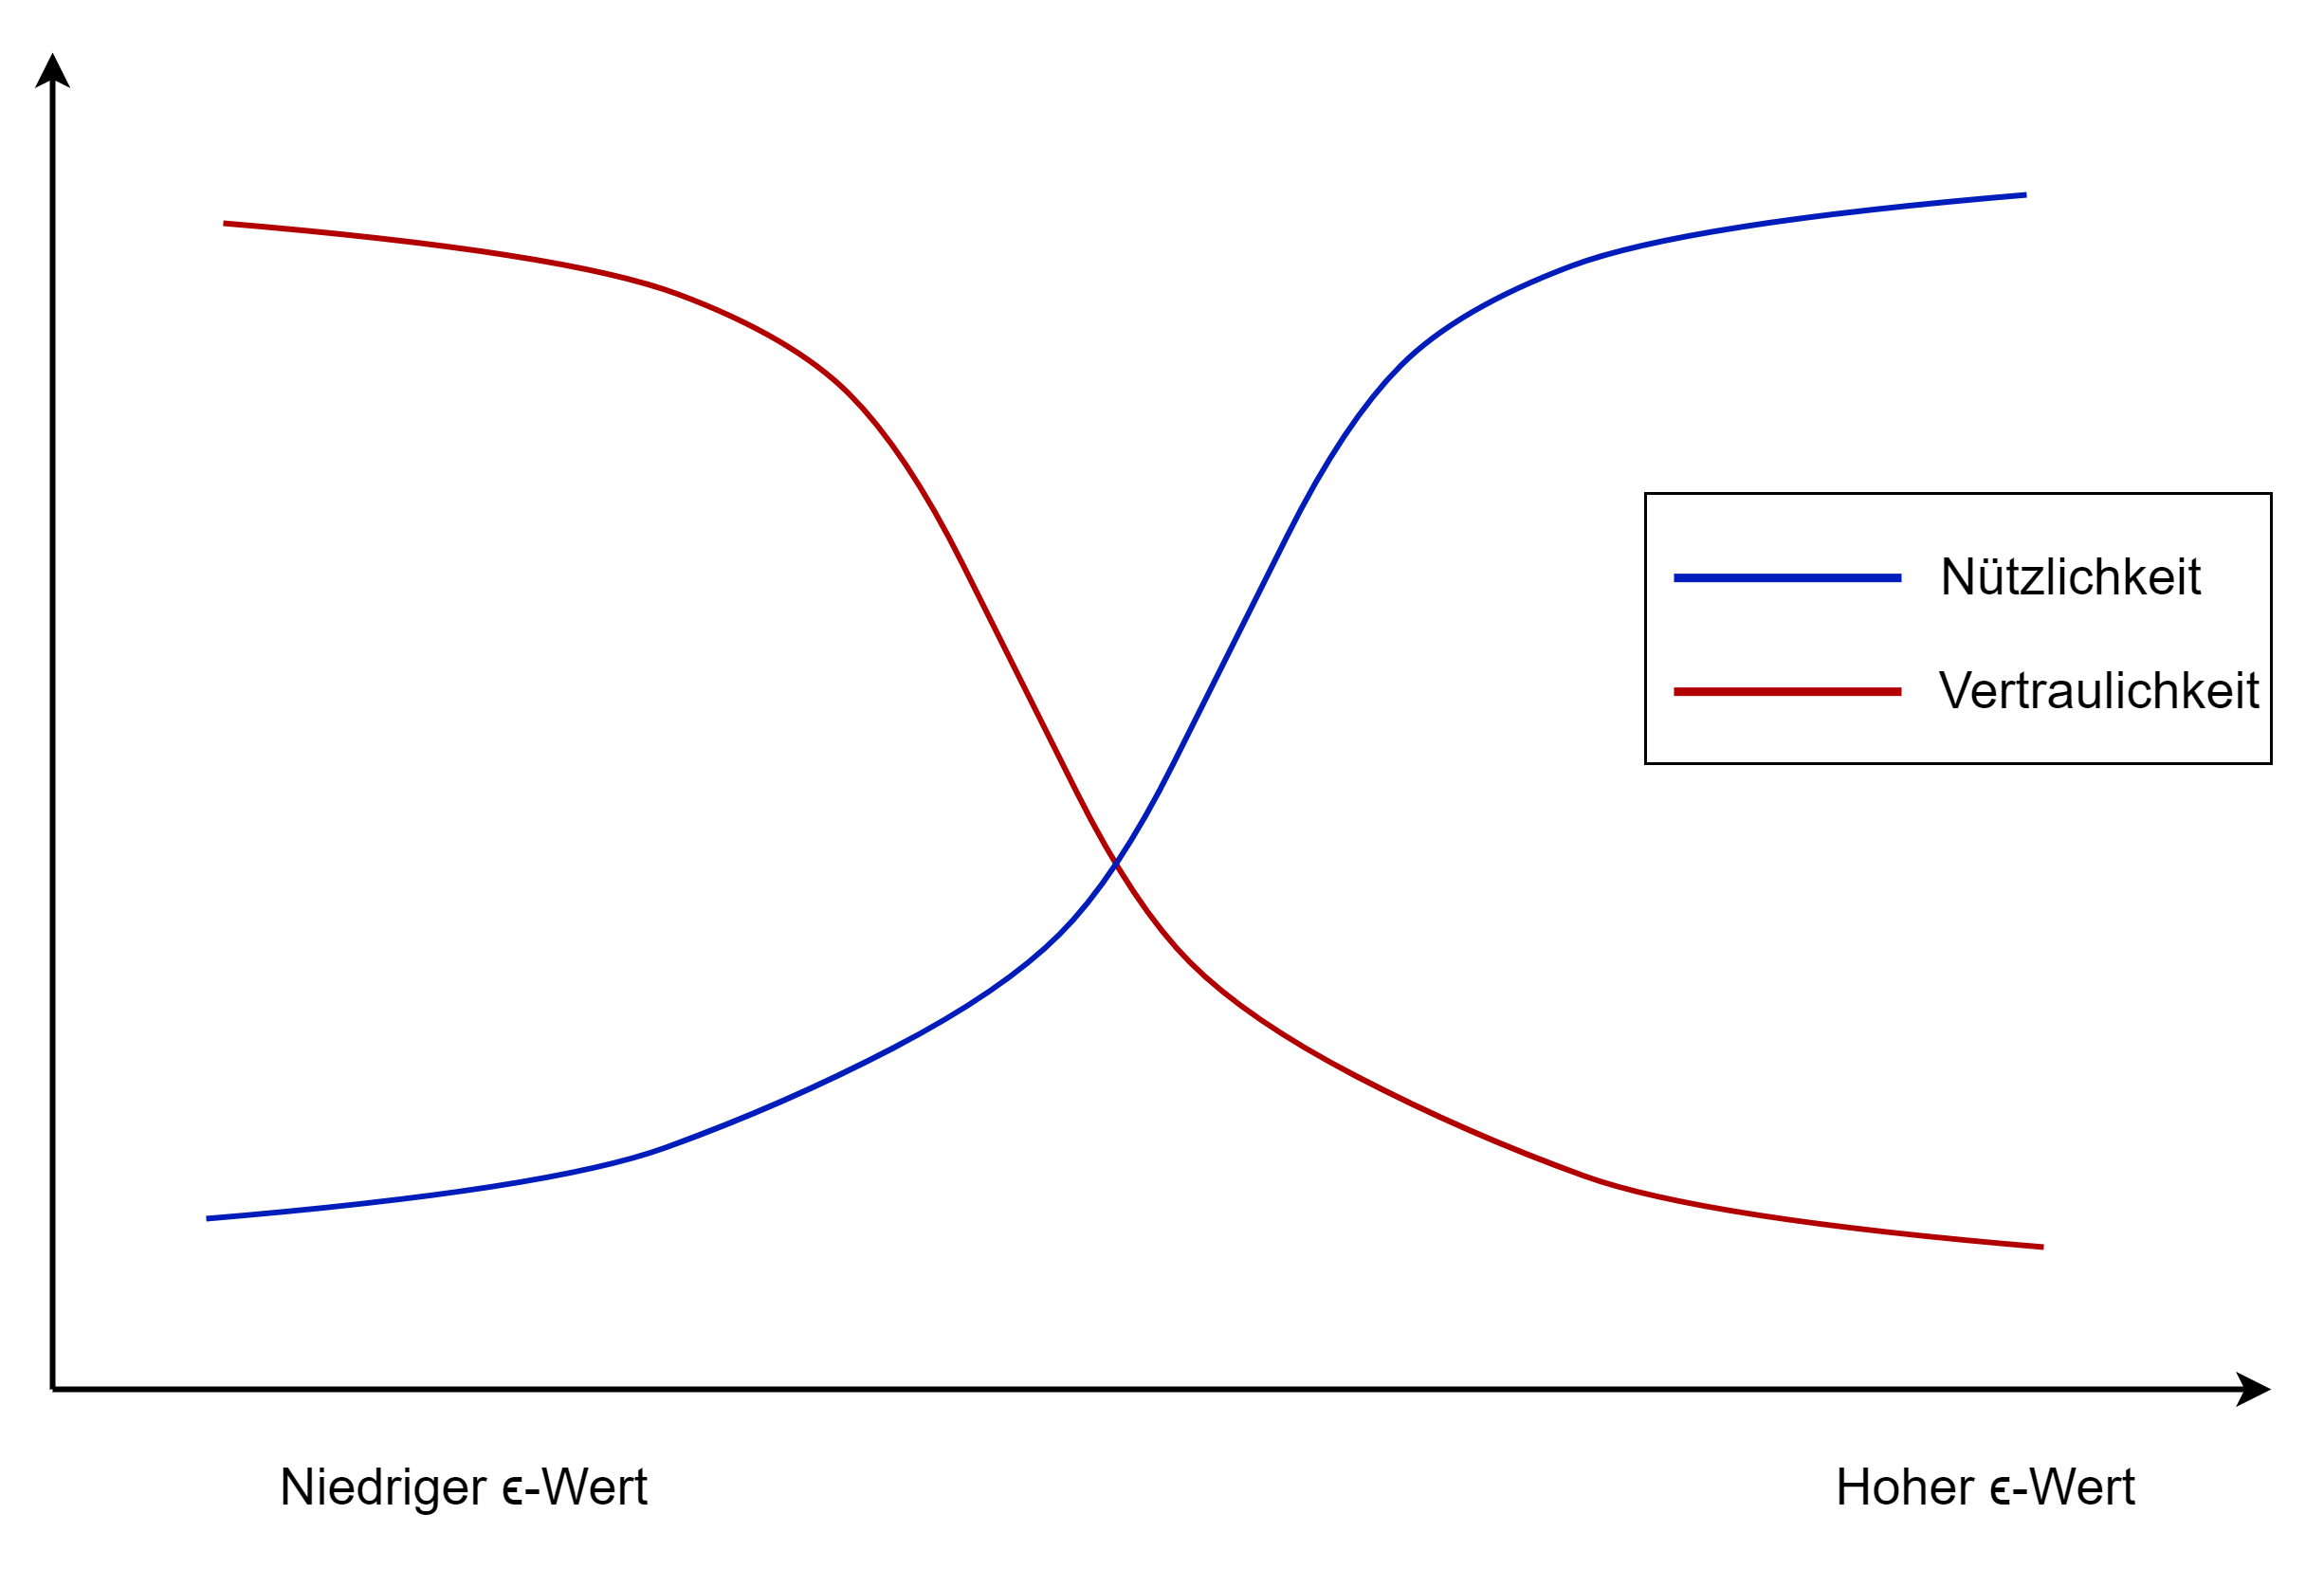
\includegraphics[width=12cm]{figures/dp_privacy_budget.png}
    \caption{Einfluss von $\epsilon$}
    \label{fig:dp_privacy_budget}
\end{figure} 

\subsubsection*{Beispiel für Differential Privacy}

Abbildung \ref{fig:dp} zeigt, wie sich Abfragen mit und ohne Differential Privacy unterscheiden.
Dabei führt ein Angreifer zunächst eine Abfrage über das Durchschnittsgehalt eines Unternehmens auf einem Datenbestand ohne Differential Privacy aus. 
Er erhält hier einen konkreten Wert als Ergebnis.
Anschließend wird der Datenbestand um einen Eintrag erweitert, weil das Unternehmen einen neuen Mitarbeiter hat.
Führt der Angreifer die Abfrage um das Durchschnittsgehalt erneut aus, erhält dieser einen angepassten, neuen Wert.
Dadurch kann er anhand der Anzahl der Mitarbeiter des Unternehmens und der Differenz der beiden Abfragen das exakte Gehalt des neuen Mitarbeiters bestimmen.
Anders sieht dies mit Differential Privacy aus. 
Dabei werden beide Abfragen mit zufälligem Rauschen angereichert. 
Es wird also nur eine Stichprobe einer Verteilung zurückgegeben. 
Bei einer gleichen Abfrage auf den gleichen Datenbestand, können also ebenfalls unterschiedliche Werte zurückgegeben werden.
Führt der Angreifer zwei Abfragen aus, einmal auf dem alten Datenbestand und auf dem Datenbestand mit dem neuen Mitarbeiter, kann er keinen exakten Wert des Gehalts des neuen Mitarbeiters ermitteln.
Differential Privacy bietet einige Algorithmen, wie dieses Rauschen hinzugefügt werden kann, wobei Parameter $\epsilon$ und $\delta$ die Stärke des Rauschens bestimmen und damit auch, wie nah die beiden Ergebnisse aneinander sind.

\begin{figure}[!htb]
    \centering
    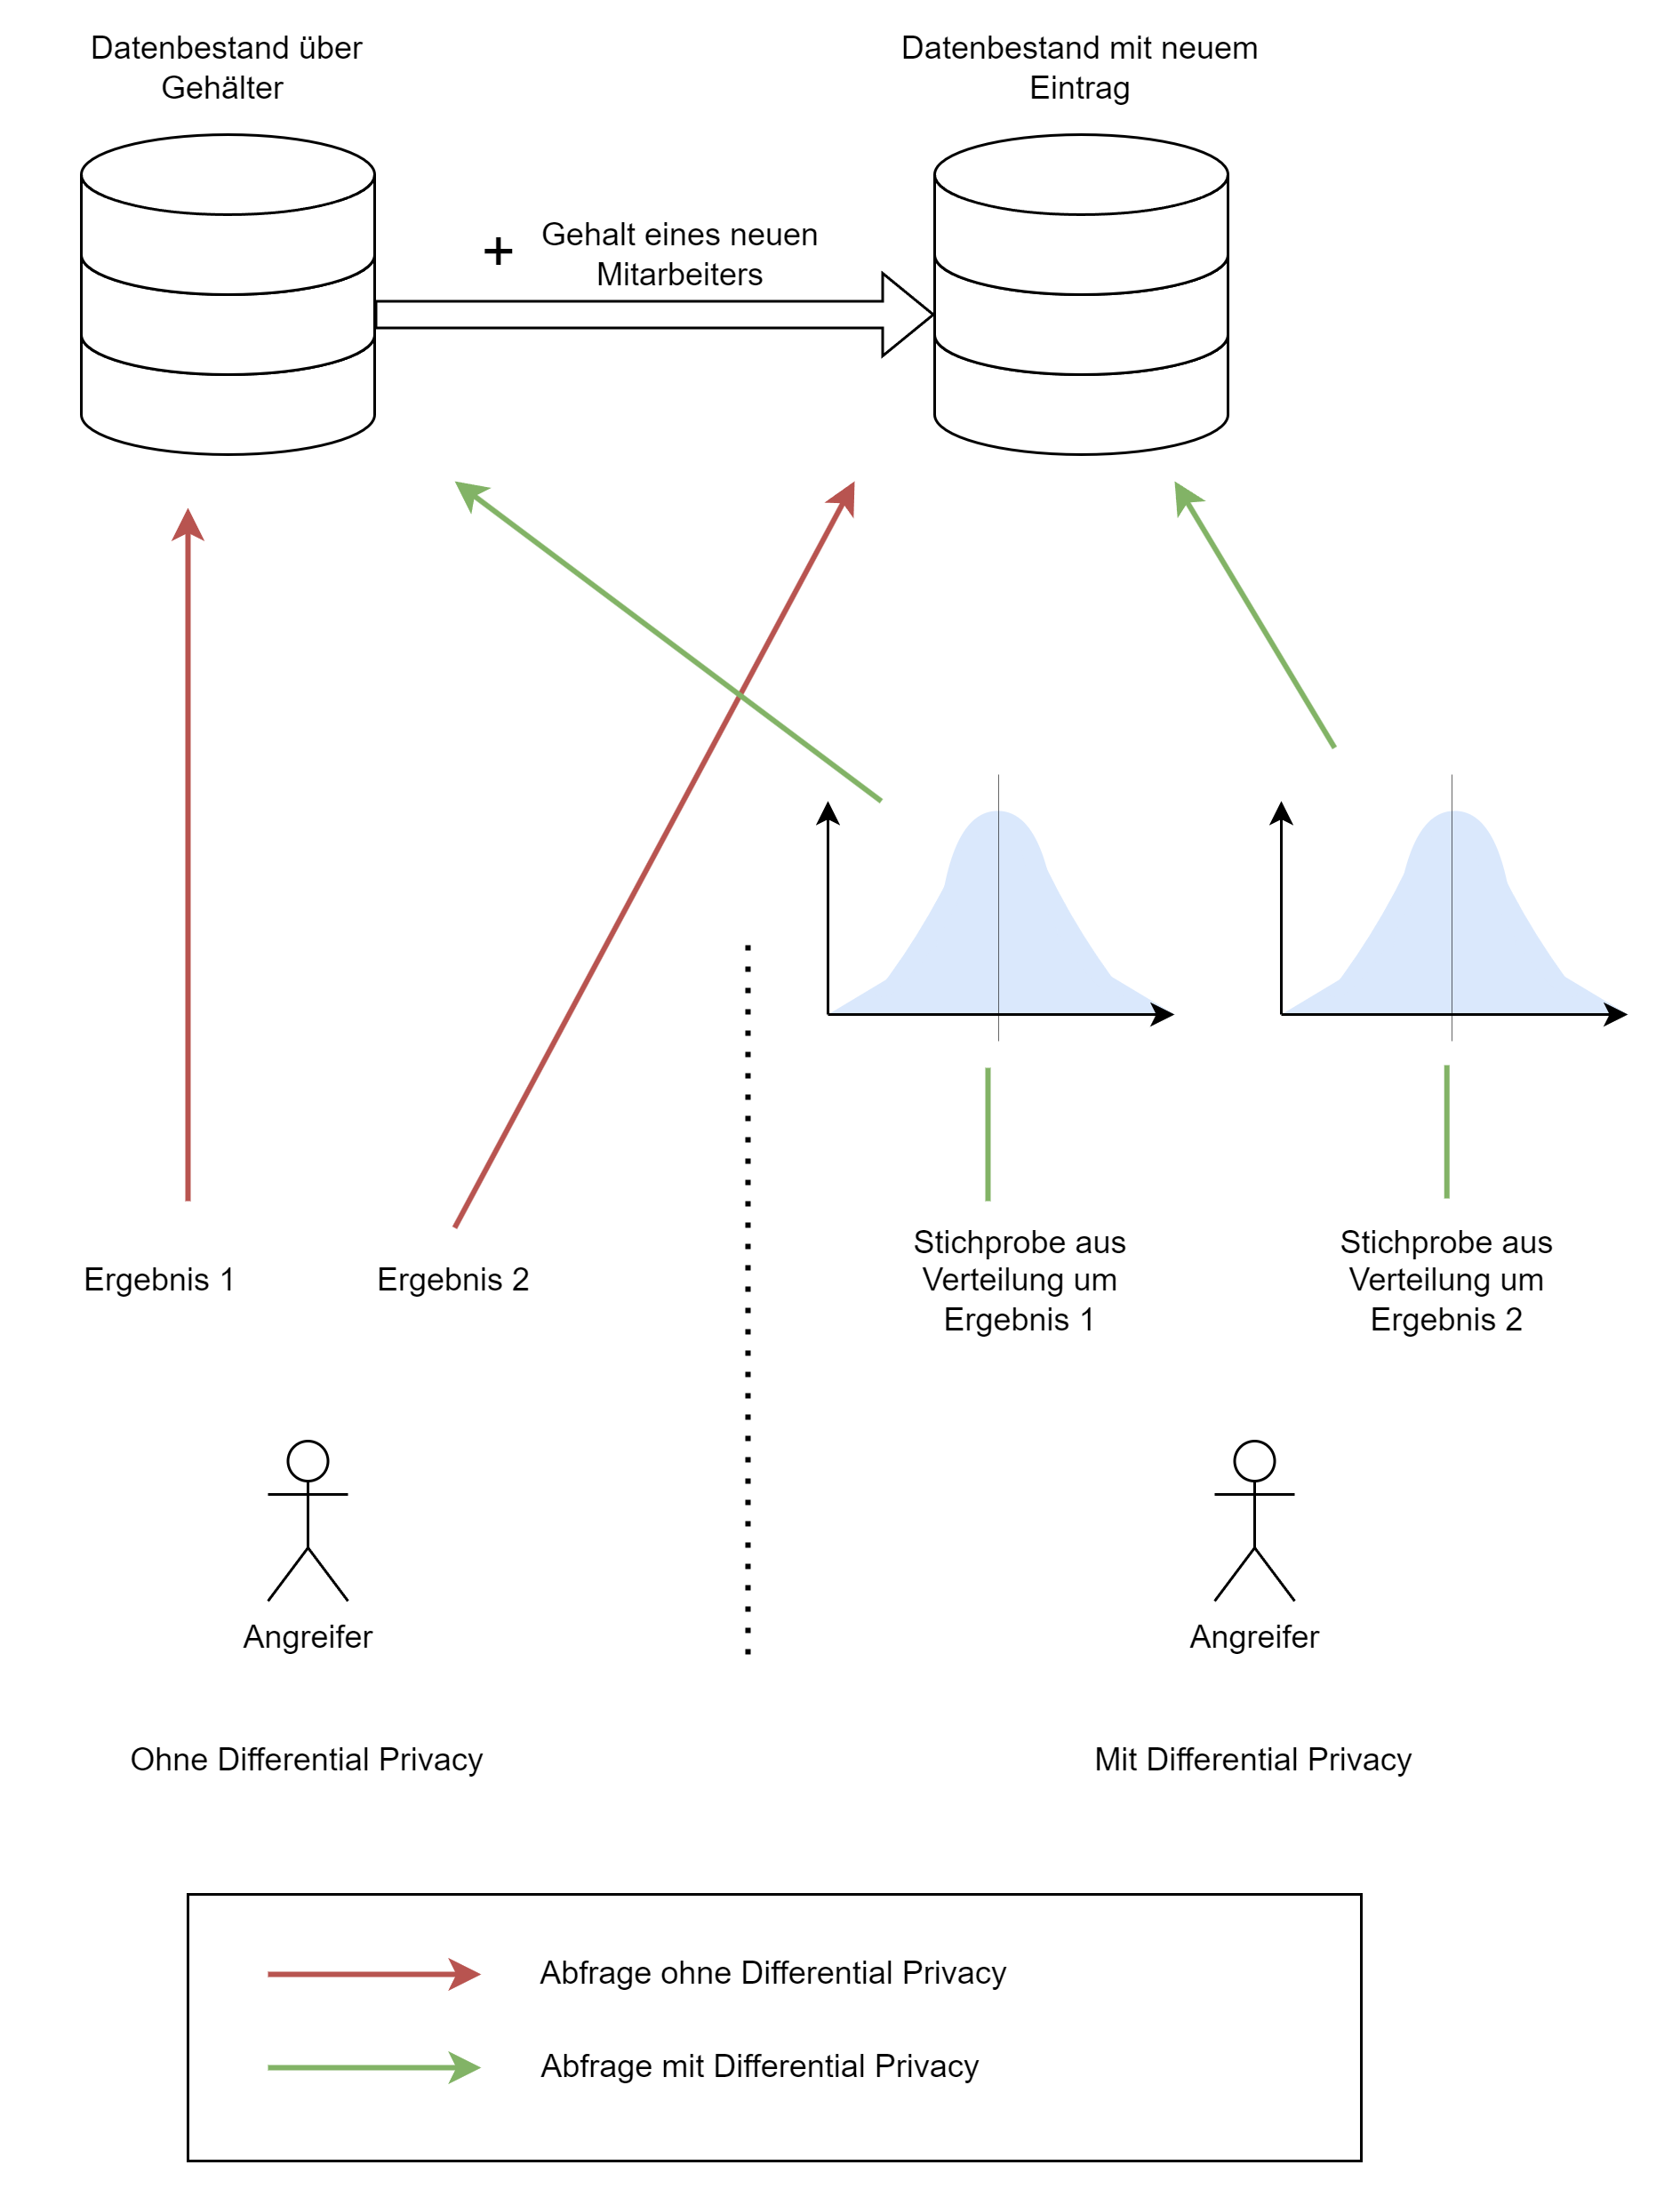
\includegraphics[width=\textwidth]{figures/dp}
    \caption{Beispiel Differential Privacy}
    \label{fig:dp}
\end{figure} 

\subsubsection*{Algorithmen für Differential Privacy}
Die Art des Rauschens, welche über die Ausgabe einer Abfrage gelegt wird, kann unterschiedlichster Herkunft sein.
Dwork und Roth \cite{P-27} stellen eine ganze Reihe dieser Mechanismen vor, die im Folgenden beschrieben werden.

Bei der Technik der randomisierten Antwort, im Englischen Random Response, wird mit einer festgelegten Wahrscheinlichkeit, ein falsches Ergebnis ausgegeben. 
Dies entspricht dem Rauschen dieser Methode.
Wird beispielsweise eine Person gefragt, ob sie eine gewisse Aktivität durchgeführt hat, wird mit 25-prozentiger Wahrscheinlichkeit die falsche Antwort selektiert.
Ist die Wahrheit \textit{\dq Ja\dq}, dann gilt $P[Antwort = \dq Ja\dq \mid Wahrheit = \dq Ja\dq] = 3/4$ und $P[Antwort = \dq Nein\dq \mid Wahrheit = \dq Ja\dq]$.
Gleiches gilt, wenn die Wahrheit \textit{\dq Nein\dq} wäre.
Die jeweils ausgegebene Antwort kann dadurch glaubhaft abgestritten werden.
\begin{equation} \label{formula:random_response}
\begin{split}
\frac{P[Antwort = \dq Ja\dq \mid Wahrheit = \dq Ja\dq]}{P[Antwort = \dq Ja\dq \mid Wahrheit = \dq Nein\dq]} = \frac{3/4}{1/4} = \\
\frac{P[Antwort = \dq Nein\dq \mid Wahrheit = \dq Nein\dq]}{P[Antwort = \dq Nein\dq \mid Wahrheit = \dq Ja\dq]} =  3
\end{split}
\end{equation}

Formel \ref{formula:random_response} zeigt, dass eine Antwort, egal ob diese \textit{\dq Ja\dq} oder \textit{\dq Nein\dq} lautet, mit einem Verhältnis von 3 abgestritten werden kann.
Der Faktor, um den sich die Wahrscheinlichkeit einer Antwort unterscheidet, wenn sich die Wahrheit ändert, liegt demnach auch bei 3.
Daraus resultiert, dass die Technik der randomisierten Antwort, mit einer 25-prozentigen Wahrscheinlichkeit einer falschen Antwort, eine ($ln 3$, 0)-Differential Privacy unterstützt.
Der natürliche Logarithmus $ln$ muss hier genutzt werden, da die Definition von Differential Privacy die Exponentialfunktion als Faktor betrachtet. 
Demnach erhält man durch $\epsilon = ln 3$ einen Unterschied um den Faktor $e^{ln 3} = 3$.

Eine weitere Technik für Differential Privacy ist der Laplace-Mechanismus.
Dabei wird das Rauschen, welches über das Ergebnis der Abfrage gelegt wird, aus einer Laplace-Verteilung ermittelt.
Eine Bedingung ist dabei, dass es sich bei dem Ergebnis der Abfrage um einen Zahlenwert handelt.
Die Dichtefunktion der Laplace-Verteilung, zentriert um den Erwartungswert $\mu=0$, mit dem Skalenparameter $\sigma$, lautet \cite{P-27}:
\begin{equation}
\resizebox{!}{0.55cm}{$
    Lap(x|\sigma) = \frac{1}{2\sigma}\times e^{(-\frac{|x|}{\sigma})}
$}
\end{equation}
wobei $\sigma$ die Steigung der Funktion beeinflusst.
Um nun ein geeignetes $\sigma$ zu wählen, muss zuerst ein Wert ermittelt werden, um den sich eine Funktion bei Änderung eines Datenpunktes maximal unterscheiden kann.
Diese sogenannte Sensitivität wird als $\Delta f$ notiert.
Geht es beispielsweise um eine Anzahl an Datensätzen, so würde ein neuer Datensatz die Anzahl um den Wert 1 erhöhen.
Folglich ist $\Delta f = 1$, denn die Anzahl wird sich durch einen neuen Datensatz um den Wert 1 verändern.
Es gibt jedoch auch Fälle, in denen der Wert der Sensitivität nicht eindeutig ist, beispielsweise bei dem obigen Gehaltsbeispiel.
Das Gehalt einer neuen Person könnte für eine beliebige Veränderung des Durchschnittsgehalts sorgen, da theoretisch jedes Gehalt möglich wäre.
Realistisch betrachtet gibt es jedoch einen Wertebereich, in dem sich alle Gehälter befinden. 
Dieser könnte beispielsweise von 0 Euro bis 10 Milliarden Euro reichen. 
Jedoch sollten die Grenzen möglichst nahe an den echten Grenzen liegen. 
10 Milliarden Euro ist theoretisch möglich, jedoch ist eine Grenze von 200.000 Euro realistischer.
Dieser Wertebereich muss also fachlich festgelegt werden.
In diesem Beispiel wäre die Sensitivität $200.000/n$, wobei $n$ die Anzahl der Mitarbeiter ist.


Um ($\epsilon$,0)-Differential Privacy zu erreichen, muss die Ausgabe einer Abfrage $M$ mit zufälligen Werte der Laplace-Verteilung $Lap(x | \Delta f/\epsilon)$ verrauscht werden \cite{P-27}: 
\begin{equation}
    M(D) = f(D) + (Y_1, ... Y_k),\text{ mit } Y_i \sim Lap(x| \Delta f/\epsilon)
\end{equation}


Eine Abwandlung des Laplace-Mechanismus ist es, anstatt der Laplace-Verteilung, eine Gaußverteilung zu nutzen. Die Dichtefunktion dieser zentriert um den Erwartungswert $\mu=0$ lautet \cite{P-27}:
\begin{equation}\label{formula:gauß}
\resizebox{!}{0.55cm}{$
    Gau\text{\textit{ß}}(x|\sigma) = \frac{1}{\sigma\sqrt{2\pi}}\times e^{-\frac{1}{2}(\frac{x}{\sigma})^2}
$}
\end{equation}
Der Gauß-Mechanismus liefert ($\epsilon$,$\delta$)-Differential Privacy, wenn $\sigma = \Delta f \frac{\text{ln}(1/\delta)}{\epsilon}$ ist \cite{P-27}.

Neben den bereits beschriebenen Mechanismen gibt es noch den Exponential-Mechanismus. 
Bei diesem wird ein Element aus einer Menge ausgegeben, welches anhand einer Bewertungsfunktion ausgewählt wird.
Die Abfrage an einen Datenbestand liefert also keine Zahl, sondern einen Datensatz oder Attributwert aus diesem.
Der Exponential-Mechanismus benötigt eine Bewertungsfunktion $u:D x R \xrightarrow{} \mathbb{R}$, welche für jede potenzielle Ausgabeoption $R$ aus einer Menge an Datensätzen $D$, einen Nutzwert im Wertebereich $\mathbb{R}$ berechnet.
Als Sensitivität $\Delta f$ entspricht der Sensitivität der Bewertungsfunktion $\Delta f = \Delta u$
Die Anfrage erfüllt dabei ($\epsilon$,0)-Differential Privacy, wenn der Mechanismus $M(D,u,R)$ ein Element $r \in R$ auswählt und ausgibt, mit einer Wahrscheinlichkeit proportional abhängig von
\begin{equation}\label{formula:exp_mech}
\resizebox{!}{0.8cm}{$
    e^{\frac{\epsilon \times u(D,r)}{2\Delta u}}
$}
\end{equation}


Als Beispiel könnte ein Mechanismus genutzt werden, welcher ausgeben soll, ob Krankheit \dq A\dq\ oder \dq B\dq\ häufiger vorkommt.
Somit wären die möglichen Optionen $R$=\{\dq A\dq,\dq B\dq\}, die Bewertungsfunktion $u(D,r)=\text{Count(r in D)}$.
Die Sensitivität ist $\Delta u = 1$, da ein zusätzlicher Datensatz die Zählung maximal um die Anzahl 1 verändern kann. 
Für jede der Optionen in $R$, würde die Ausgabewahrscheinlichkeit mit Formel \ref{formula:exp_mech} berechnet werden. 
Anschließend gibt der Mechanismus entweder \dq A\dq\ oder \dq B\dq\ zurück, abhängig der zuvor berechneten Ausgabewahrscheinlichkeiten.
Das Rauschen des Exponential-Mechanismus ist demnach, dass nicht immer die Option $r \in R$ mit dem größten Nutzwert ausgegeben wird. 

Eine alternative Möglichkeit, neben dem Exponential-Mechanismus, einen Wert aus einem Datensatz mittels Ausgabewahrscheinlichkeiten zu bestimmen, ist die sogenannte Report Noisy Max Methode. 
Dabei werden die echten Wahrscheinlichkeitswerte mittels Laplace-Mechanismus verrauscht und anschließend wird der Wert oder Datenpunkt mit der höchsten Wahrscheinlichkeit selektiert.


\subsubsection*{Eigenschaften von Differential Privacy}
Das Ziel von Differential Privacy, die Vertraulichkeit eines Datensatzes zu schützen und dennoch die Nützlichkeit des Datenbestands zu bewahren, wurde bereits zu Beginn des Kapitels geschildert.
Jedoch bringt Differential Privacy eine Reihe weiterer nützlicher Eigenschaften mit sich \cite{P-27}:
\begin{compactitem}
    \item \textbf{Gruppen Privacy:} Differential Privacy betrachtet zwei Datenbestände, die sich in einem Datensatz unterscheiden. Jedoch gelten die gleichen Regeln für Datenbestände, die sich in mehreren Datensätzen unterscheiden, wobei $\epsilon$ dabei mit der Anzahl der unterschiedlichen Datensätze multipliziert wird.
    \item \textbf{Resistenz gegen Umkehrung bei der Weiterverarbeitung:} Das Ergebnis eines Mechanismus, welcher Differential Privacy nutzt, ist geschützt und es gibt keinen Mechanismus, welcher dies umkehren könnte. Somit sind geschützte Weiterverarbeitungen der Ergebnisse möglich.
    \item \textbf{Quantifizierung der Vertraulichkeit:} Mit den Parametern $\epsilon$ und $\delta$ kann angegeben werden, wie stark die Vertraulichkeit der Daten geschützt wird.
    \item \textbf{Bewertung zusammengesetzter Mechanismen:} Durch die Quantifizierung der Vertraulichkeit, können auch zusammengesetzte und parallele Berechnungen bewertet werden.
\end{compactitem}



Die Bewertung von mehreren zusammengesetzten Mechanismen ist dabei komplex und kann für bestimmte Berechnungen verfeinert werden \cite{P-27}. 
Der dabei berechnete $\epsilon$-Wert ist eine Obergrenze, welcher durch bestimmte Restriktionen und Berechnungen noch genauer definiert werden kann.
Grundlegend jedoch, besitzt ein Mechanismus, welcher aus nacheinander ausgeführten Teilmechanismen besteht, einen $\epsilon$-Wert und $\delta$-Wert, welcher der Summe aus den einzelnen Teilmechanismen entspricht.
Erfüllt $M_1(D)$ eine $(\epsilon_1,\delta_1)$-Differential Privacy und $M_2(D)$ eine $(\epsilon_2,\delta_2)$-Differential Privacy, dann erfüllt der gesamte Mechanismus $(\epsilon_1 + \epsilon_2,\delta_1 + \delta_2)$-Differential Privacy.
Wird ein und derselbe Teilmechanismus mit $(\epsilon,\delta)$-Differential Privacy $t$ mal ausgeführt, so entspricht der Gesamtmechanismus $(t\epsilon,t\delta)$-Differential Privacy.
Zusammengefasst lässt sich dies durch folgende Definition beschreiben \cite{P-27}:\\
\textit{
    Wenn ein Mechanismus $M_{|t|}$, aus $t$ Teilmechanismen $M_i$ mit $(\epsilon_i,\delta_i)$-Differential Privacy besteht, dann erfüllt dieser  ($\Sigma_{i=1}^{t} \epsilon_i $, $\Sigma_{i=1}^{t} \delta_i $)-Differential Privacy
}

Alternativ kann ein Mechanismus auch aus Teilmechanismen bestehen, welche jeweils nur auf einer disjunkten Menge an Datensätzen des gesamten Datenbestands ausgeführt wird.
Der gesamte Mechanismus hat als $\epsilon$ und $\delta$-Wert dabei die maximalen Werte der Teilmechanismen.\\
\textit{
    Wenn ein Mechanismus $M_{|t|}$, aus $t$ Teilmechanismen $M_i$ mit $(\epsilon_i,\delta_i)$-Differential Privacy besteht, welche jeweils 
    nur auf einer disjunkten Menge an Datensätzes des gesamten Datenbestands $D_i$ ausgeführt werden, 
    dann erfüllt dieser Mechanismus ($max_i(\epsilon_{i})$, $max_i(\delta_{i})$)-Differential Privacy
}


Ein Beispiel für einen Algorithmus, welcher eine angepasste Bewertung von zusammengesetzten Mechanismen besitzt, ist der Trainingsalgorithmus DPSGD (Kapitel \ref{sec:dp_training}) \cite{P-28}.
Diese Anpassung sorgt dafür, dass der $\epsilon$-Wert über den ganzen Trainingsprozess möglichst niedrig bleibt.
Ziel davon ist es, eine Obergrenze für $\epsilon$ zu beschreiben, welche näher an den tatsächlichen Berechnungen liegt, als das Aufsummieren der einzelnen $\epsilon$ Werte.


\subsubsection*{Vorverarbeitung der Trainingsdaten}
Um die Trainingsdaten eines Modells mit Differential Privacy zu schützen, ist es möglich, die Daten vor der Eingabe in das Modell zu verrauschen.
Der Forward-Pass eines Modells wird demnach nicht auf den echten Daten ausgeführt, sondern auf den jeweils verrauschten Versionen der einzelnen Datensätze.

Um einen einzelnen Datensatz zu verrauschen, muss jedes Attribut des Datensatzes individuell betrachtet werden. 
Dabei ist die Sensitivität individuell zu setzen, beeinflusst von statistischen Merkmalen des Attributes.
Ebenfalls kann sich der Differential Privacy Mechanismus unterscheiden, abhängig davon, ob es sich um kategoriale oder numerische Werten handelt.
Bei numerischen Werten kann der Laplace-Mechanismus oder Gauß-Mechanismus gewählt werden, bei kategorialen Werten der Exponential-Mechanismus.
Der $\epsilon$-Wert und $\delta$-Wert eines einzelnen Datenpunktes entspricht anschließend der Summe der Werte des einzelnen Verrauschens jeder Variable.

Da jeder Datensatz alleine eine disjunkter Menge des Datenbestands darstellt, gilt, dass der $\epsilon$-Wert und $\delta$-Wert dem Maximum des Rauschens auf die einzelnen Datensätze entspricht.
Wird also jeder Datensatz mit dem gleichen, festgelegten Mechanismus mit ($\epsilon$,$\delta$)-Differential Privacy verrauscht, dann entspricht dies auch den Werten des gesamten Vorverarbeitungsprozess.

Alternativ kann ein ganzer Datenbestand mit Differential Privacy geschützt werden, indem dieser nur dazu genutzt wird, einen synthetischen Datenbestand zu erzeugen.
Dieser kann anschließend wie der originale Datenbestand genutzt werden.
Das folgende Kapitel stellt einige Methoden dazu vor.


\subsection{Synthetische Daten}\label{sec:synthetic_data}

Bei einem synthetischen Datenbestand handelt es sich um einen künstlich erzeugten Datenbestand, welcher die gleichen statistischen Merkmale wie der ursprüngliche Datenbestand enthält.
Statistische Abfragen oder auch komplexere Modelle, wie neuronale Netze, sollen demnach bei beiden Datenbeständen vergleichbare Ergebnisse liefern.

Bisher wurde Differential Privacy für einzelne Abfragen genutzt.
Es gibt jedoch auch Verfahren, welche es ermöglichen, eine synthetische Menge an Datensätzen zu veröffentlichen, welcher mit Differential Privacy geschützt werden.
Hardt \etal \cite{P-90} stellen solch ein Verfahren vor, welches MWEM genannt wird.
Dieses basiert auf Marginalverteilungen, auch Randverteilungen genannt, von verschiedenen Attributen zueinander.
Dabei handelt es sich um Anzahlen verschiedener Attributwerte eines Attributs in Kombination mit den Anzahlen verschiedener Attributwerte eines anderen Attributes.
Einzelne Werte der Marginalverteilungen werden auch Marginalhäufigkeiten genannt.
Tabelle \ref{tab:marginals} zeigt, wie ein Beispiel von Marginalverteilungen zwischen den Attributen \dq A\dq\ und \dq B\dq, welche jeweils zwei unterschiedliche Attributwerte annehmen können.
Stetige Werte müssten vorher in verschiedene Klassen gruppiert werden.

\input{tables/marginalverteilungen}

Um eine Datenmenge umzuwandeln, wird eine Datenmenge $D'$ mit der gleichen Anzahl an Elementen wie die ursprüngliche Datenmenge $D$ initialisiert, wobei die Initialwerte der Attribute mittels einer Gleichverteilung über alle potenziellen Attributwerte des jeweiligen Attributes ermittelt werden.
Das Verfahren besteht aus 3 Schritten, welche iterativ wiederholt werden können, um die künstliche Datenmenge $D'$ an die echte Datenmenge $D$ anzugleichen:
\begin{compactenum}
    \item \textbf{Wahl einer Anfrage:} Aus allen Marginalhäufigkeiten der ursprünglichen Datenmenge, wird mittels Exponential-Mechanismus die Marginalhäufigkeit gewählt, die den größten Unterschied zwischen den Eingaben $D'$ und $D$ besitzt.
    Die Bewertungsfunktion $u$ des Exponential-Mechanismus bewertet folglich die Differenzen der Marginalverteilungen der beiden Datenmengen (originale Datenmenge und synthetische Datenmenge).
    \item \textbf{Verrauschen:} Mittels Laplace-Mechanismus wird nun das Ergebnis der gewählten Marginalverteilung aus Schritt 1 verrauscht.
    \item \textbf{Anpassen von $D'$:} Abhängig von dem verrauschten Ergebnis der gewählten Marginalverteilung, werden die Attributwerte von $D'$ so angepasst, dass die Marginalverteilungen sich angleichen.
\end{compactenum}
Nach Beendigung des Algorithmus, ist $D'$ eine synthetische Datenmenge, welche die originale Datenmenge $D$ mit Differential Privacy abbildet.

Die Erzeugung synthetischer Daten wurde im Jahre 2016 maßgeblich durch die Generative Adversarial Network Architektur, auch GAN genannt, beeinflusst \cite{P-86}. 
Bei dieser Architektur gibt es zwei gegensätzliche neuronale Netzwerke, der Generator und der Diskriminator. 
Der Diskriminator lernt dabei, zwischen echten Daten und nicht echten Daten zu unterscheiden, welche abwechselnd von dem echten Datenbestand und von dem Generator kommen.
Im Gegensatz dazu, versucht der Generator, Datensätze zu erzeugen, die den Diskriminator täuschen. 
Der Diskriminator kann dabei zwei Verlustfunktionen haben, einmal für sich selber und einmal für den Generator.
Die Verlustfunktion des Generators kann dabei durch den Generator backpropagiert werden, wodurch dieser immer realistischere Datensätze generiert.
Im besten Falle, erzeugt der Generator nach dem Training Datensätze, die so echt wirken, dass der Diskriminator diese nicht mehr unterscheiden kann.
Folglich erzeugt der Generator synthetische Daten, welche die statistischen Strukturen der originalen Daten enthalten.
Abbildung \ref{fig:gan} zeigt die bereits beschriebene Architektur.

\begin{figure}[!htb]
    \centering
    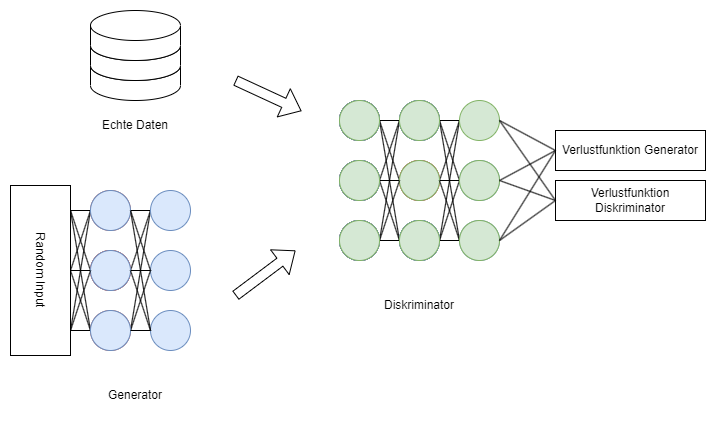
\includegraphics[width=14cm]{figures/gan}
    \caption{Generative Adversarial Network nach \cite{P-86}}
    \label{fig:gan}
\end{figure} 

Die Erzeugung von Daten mittels GANs kann nicht nur für Angriffe genutzt werden (siehe Kapitel \ref{sec:angriffe}), sondern auch für das Training von neuronalen Netzen.
Eine Erweiterung der GANs ist das sogenannte Wasserstein GAN oder auch kurz WGAN \cite{P-92}. 
Standardmäßig kann bei GANs der Fall auftreten, dass die erzeugten Daten nicht jeden Teil einer Verteilung abbilden, sondern nur einen Teil, \zB den am häufigsten vorkommenden Datensatz.
Um dieses Problem zu mindern, wird beim WGAN die Verlustfunktion des Diskriminators verändert. 
Anstatt einer binären Klassifikation (echt oder unecht), wird die Wasserstein-Distanz genutzt, welche angibt, wie viel Arbeit benötigt wird, um eine Verteilung in eine andere Verteilung zu transformieren. 
Die Wasserstein-Distanz gleicht der Earth-Mover-Distanz aus Kapitel \ref{sec:anonymisierung}.
Diese Metrik als Verlustfunktion ist jedoch nur nützlich, wenn nicht mit einzelnen Datensätzen, sondern jeweils mit Batches trainiert wird.
Der Austausch der Verlustfunktion sorgt dafür, dass der Generator Daten aus der ganzen Verteilung der Daten nachstellen muss und nicht nur aus einem Teil dieser.


Xie \etal \cite{P-70} stellen eine besondere Form des GANs vor, das sogenannte Differentially Private Generative Adversarial Network oder kurz DPGAN.
Dieses DPGAN nutzt als Basis das WGAN, fügt jedoch bei Berechnung der Verlustfunktion (Wasserstein-Distanz) Rauschen mittels des Gauß-Mechanismus aus Kapitel \ref{sec:dp} hinzu.
Durch die Eigenschaft, dass Differential Privacy resistent gegenüber Nachbearbeitung ist, kann auch garantiert werden, dass die Gradienten, die im Generator ankommen, mittels Differential Privacy geschützt sind.
Die Autoren können zeigen, dass es möglich ist, Bilder der MNIST Datenmenge \cite{D-MNIST} zu erzeugen.
Abbildung \ref{fig:dpgan} zeigt diese Erzeugung mit unterschiedlichen $\epsilon$ Werten.
Es ist zu sehen, dass bei kleiner werdendem $\epsilon$, die Qualität der Bilder schlechter wird und auch mehr Daten der falschen Klasse erzeugt werden. 
Bei $\epsilon=9,6$ ist die Anzahl an Daten mit falschem Label größer, als die Anzahl der Daten mit richtigem Label.
Folglich ist die Wahl von $\epsilon$ entscheidend, wie gut die synthetischen Daten die Originaldaten wiedergeben.
Die Wahl muss von $\epsilon$ muss dabei für jeden Use Case neu evaluiert werden.

\begin{figure}[!htb]
    \centering
    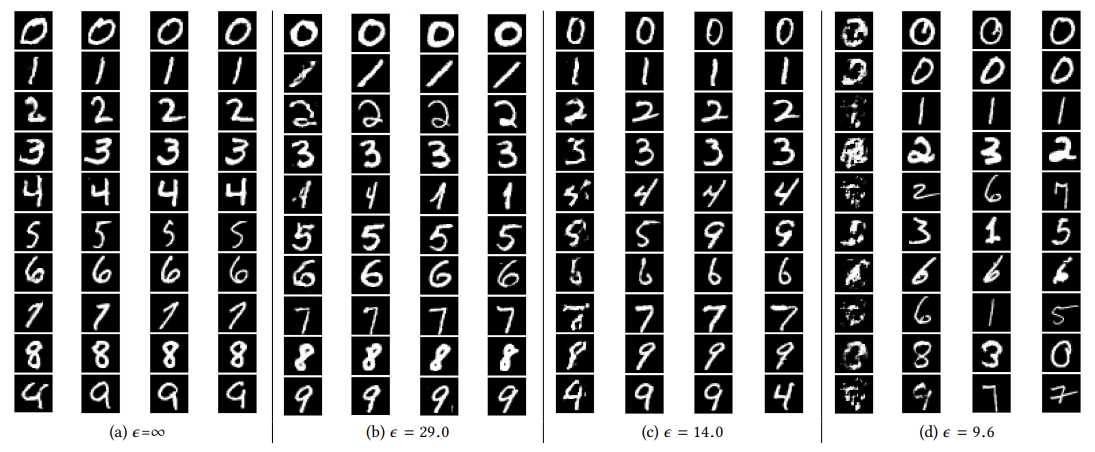
\includegraphics[width=\textwidth]{figures/dpgan}
    \caption{Synthetische MNIST Datenmenge mittels DPGAN \cite{P-70}}
    \label{fig:dpgan}
\end{figure} 

Jordon \etal \cite{P-68} stellten eine alternative Form des GANs vor, welches ebenfalls synthetische Daten erzeugt. 
Dieses nutzt das Private Aggregation of Teacher Ensembles Framework, kurz PATE, welches in Kapitel \ref{sec:pate} im Detail beleuchtet wird.
Bei der PATE-Architektur wird der Datenbestand in verschiedene Teildatenmengen unterteilt. 
Verschiedene Modelle, die sogenannten Lehrer oder Teacher Modelle, lernen die Klassifikation jeweils an einer der unterschiedlichen Teildatenmengen.
Ein weiteres Modell, welches Schüler oder Student Modell genannt wird, kann nun mittels des Exponential-Mechanismus aus \ref{sec:dp} aus den aggregierten Vorhersagen der Lehrer Modelle, eine Klasse vorhersagen.
Das PATE-GAN nutzt die PATE-Architektur für den Diskriminator, welcher ein binärer Klassifikator ist.
Wie das DPGAN, nutzt auch das PATE-GAN die Resistenz gegenüber Nachbearbeitungen von Differential Privacy aus, um Differential Privacy auch für die synthetischen Daten zu garantieren.


Ein weiterer Algorithmus, welcher kein GAN zur Erzeugung künstlicher Daten nutzt, ist NIST-MST von McKenna \etal \cite{P-95}.
Mit NIST-MST gewannen McKenna \etal die \textit{Differential Privacy Synthetic Data Competition}, welche vom National Institute of Standards and Technology der USA ausgetragen wurde.
Neben NIST-MST, welcher auf den obigen Wettbewerb angepasst wurde, gibt es noch MST für generelle Anwendungsfälle.
Die MST Methode basiert, wie MWEM \cite{P-90}, auf Marginalverteilungen.
MST besteht dabei aus 3 Schritten \cite{P-95}:
\begin{compactenum}
    \item \textbf{Wahl von Marginalverteilungen:} Aus dem Datenbestand, über den synthetische Daten erzeugt werden, können mehrere Marginalverteilungen gewählt werden. Dabei sollten die wichtigsten Zusammenhänge und Abhängigkeiten des Datenbestands in diesen vorkommen. Es wird deshalb empfohlen, dass ein Fachexperte die Marginalverteilungen aussucht.
    \item \textbf{Zählen der Marginalverteilungen:} Marginalverteilungen enthalten die Anzahl von Attributwerten eines Attributes in Abhängigkeit von den Attributwerten eines anderen Attributes. Um die Vertraulichkeit der Daten mittels Differential Privacy zu schützen, werden die unterschiedlichen Anzahlen der Variablen mittels Gauß-Mechanismus verrauscht.
    \item \textbf{Erzeugung der Daten:} MST nutzt ein Tool namens Private-PGM \cite{P-97}, welches von den gleichen Autoren stammt, um einen künstlichen Datenbestand zu erzeugen. Dabei sollen die Marginalverteilungen des künstlichen Datenbestands möglichst nahe an den gemessenen Marginalverteilungen liegen.
\end{compactenum}
Die MST Methode ähnelt der MWEM Methode, jedoch gibt es einige Unterschiede.
MWEM ist ein iterativer Algorithmus, welcher in jeder Iteration die Marginalhäufigkeit mit der größten Differenz zwischen originalem Datenbestand $D$ und synthetischem Datenbestand $D'$ wählt und die Attributwerte des synthetischen Datenbestands so anpasst, dass diese sich der Marginalhäufigkeit des originalen Datensatzes angleicht.
MST hingegen stellt mit dem Tool Private-PGM \cite{P-97} ein Optimierungsproblem auf, welches versucht, einen Datenbestand zu finden, dessen Marginalverteilungen möglichst Nahe an den gemessenen Marginalverteilungen des originalen Datenbestands liegt.
\section{Training des Modells}\label{sec:training_modells}

Das Training eines Neuronalen Netzes bietet eine Vielzahl an Anknüpfungspunkten, um die Vertraulichkeit der Daten zu sichern.
Der für das Training leichteste Fall ist es, wenn bereits bei der Vorverarbeitung der Daten ein Mechanismus angewendet wurde, der die Vertraulichkeit schützt.
Dies sorgt dafür, dass das Training ohne Anpassung stattfinden kann.
Alternative Methoden, welche im Folgenden detailliert erläutert werden, beeinflussen die Algorithmen der Trainingsmethodik, verändern die Architektur des Modells oder verschlüsseln das gesamte Modell.


\subsection{Training mit Differential Privacy}\label{sec:dp_training}

Nachdem Kapitel \ref{sec:dp} bereits zeigt, wie Differential Privacy definiert wird und bei der Vorverarbeitung von Daten genutzt werden kann, behandelt das folgende Kapitel, wie Differential Privacy während des Trainings genutzt werden kann.

Abadi et al. \cite{P-28} zeigen, wie der Trainingsalgorithmus angepasst wird, um Differential Privacy zu unterstützen.
Die Methode trägt den Namen Differentially private SGD oder auch DPSGD.
Ein Trainingsschritt mittels DPSGD sieht dabei wie folgt aus:
\begin{compactenum}
    \item Ein Batch von zufälligen Daten wird als Input des Modells für den Feedforward Schritt genutzt. Dabei kommt jeder Datenpunkt mit der gleichen Wahrscheinlichkeit in einem Batch vor. Anders als bei einem normalen Training könnten einzelne Datensätze auch mehrmals oder gar nicht innerhalb einer Epoche zum Trainieren genutzt werden. 
    \item Die Gradienten werden mittels der Verlustfunktion berechnet. Dies gleicht dem Training ohne Differential Privacy.
    \item Die maximale Größe der Gradienten wird beschränkt. Dies liegt daran, dass Gradienten potenziell beliebig groß werden könnten, was dafür sorgen könnte, dass das berechnete Privacy Budget nicht eingehalten werden könnte.
    \item Anschließend werden die Gradienten durch den Gauß-Mechanismus verrauscht. 
    \item Die Anpassung der Gewichte erfolgt in die umgekehrte Richtung der Gradienten, skaliert mit einer Lernrate. Dies gleicht ebenfalls dem normalen Trainingsvorgehen.
\end{compactenum}

Ein wichtiger Teil der Methode ist jedoch die Berechnung des $\epsilon$-Werts und des $\delta$-Werts über den Trainingsprozess hinweg.
Hierbei wird für jeden Batch berechnet, welchen Einfluss dieser über die Gradienten auf die Gewichte des Modells hat.
Das Rauschen in Schritt 4 wird dabei so gewählt, dass eine Anpassung der Gewichte durch einen Batch ($\epsilon$,$\delta$)-Differential Privacy erfüllt.
Dadurch, dass ein Batch aus zufälligen Datenpunkten des Datensatzes besteht, kann das sogenannte Privacy Amplification Theorem genutzt werden \cite{P-107}. 
Dieses besagt, dass jede Anpassung in Bezug auf den ganzen Datenbestand ($\mathcal{O}(q\epsilon)$,$q\delta$)-Differential Privacy erfüllt, wobei $q$ dem Strichprobenverhältnis von Batch Größe zu Datensatzgröße entspricht und $\mathcal{O}$ dabei der Big-$\mathcal{O}$-Notation.
Die Big-$\mathcal{O}$-Notation zeigt hier, dass das Privacy Budget höchstens so schnell wächst, wie das Stichprobenverhältnis $q$ mit dem $\epsilon$-Wert eines Batches.
Um nun mehrere Trainingsschritte zu bewerten, könnte das Privacy Budgets eines Schritts mit der Anzahl der Schritte $T$ multipliziert werden. 
Dadurch erfüllt der Trainingsprozess ($\mathcal{O}(q\epsilon T)$,$q\delta T$)-Differential Privacy.

Bei der beschriebene Berechnung des Privacy Budgets, handelt es sich um eine Obergrenze, welche mathematisch bewiesen werden kann.
Es ist jedoch vorteilhaft, eine beweisbare Obergrenze zu finden, welche möglichst nahe an dem tatsächlichen Wert liegt. 
Dies sorgt dafür, dass mehr Rauschen eingefügt werden kann, jedoch die Quantifizierung des Privacy Budgets den gleichen Wert annimmt, was wiederum die tatsächliche Privatsphäre der Daten mehr schützt.
Eine Möglichkeit die Distanz der berechneten Obergrenze bei DPSGD zu minimieren, ist das Strong Composition Theorem \cite{P-27}.
Dabei handelt es sich um ein Theorem, welches dafür sorgt, dass das Privacy Budget über mehrere Schritte geringer ansteigt, primär dadurch, dass nicht mehr mit der Anzahl der Schritte $T$ multipliziert werden muss, sondern nur mit der Wurzel davon.
Formell erfüllt der Trainingsprozess ($\mathcal{O}(q\epsilon \sqrt{T log(1/\delta)})$,$q\delta T$)-Differential Privacy.

Abadi et al. \cite{P-28} zeigen jedoch, dass die Obergrenze sogar noch geringer gesetzt werden kann, als mit dem Strong Composition Theorem.
Diese Methode wird Moment Berechnung genannt und sorgt dafür, dass der Trainingsprozess mit DPSGD ($\mathcal{O}(q\epsilon \sqrt{T})$,$\delta$)-Differential Privacy erfüllt.
Da $\delta$ normalerweise kleiner gesetzt wird, als die Inverse der Anzahl an Datensätzen im Datenbestand, sorgt das Wegfallen des Terms $\sqrt{log (1/\delta)}$ im $\epsilon$-Teil, für eine signifikante Verkleinerung des Privacy Budgets über den Trainingsprozess hinweg.
Zusätzlich entfällt im $\delta$-Teil der Faktor $qT$, wodurch der gesetzte $\delta$-Wert über den Trainingsprozess konstant bleibt.
\subsection{Private Aggregation of Teacher Ensembles PATE}\label{sec:pate}
\subsection{Homomorphe Verschlüsselung}\label{sec:homomorphe_verschlüsselung}

Homomorphe Verschlüsselung ist eine Methodik, um Berechnung auf verschlüsselten Daten durchführen zu können. Dadurch können Daten beispielsweise in der Cloud verarbeitet werden, ohne dass es dem Anbieter des Services möglich ist, die Vertraulichkeit der Daten zu gefährden.

Ein Homomorphismus in der Algebra bezeichnet eine strukturerhaltende Abbildung einer Mengen $G$ in eine andere Menge $H$.
Dabei hat jedes Element $g \in G $ mindestens ein Bild $h \in H$ und die Relationen der Elemente $g \in G$ zueinander, finden sich auch in H wieder \cite{B-2}.

Ein typisches Beispiel ist der Homomorphismus zwischen zwei Gruppen $(G,\circ)$ und $(H,\ast)$, wobei $\circ$ und $\ast$ jeweils eine Verknüpfung innerhalb der Gruppe symbolisieren. 
Die Beziehung der beiden Gruppen wird Gruppenhomomorphismus genannt, wenn es eine Funktion $f:G\to H$ gibt, die Elemente der Gruppe $G$ auf die Gruppe $H$ abbildet und dabei für alle Elemente $g_1,g_2 \in G$ gilt \cite{P-98}:
\begin{equation*}
    f(g_1 \circ g_2) = f(g_1) \ast f(g_2)
\end{equation*}
Abbildung \ref{fig:group_homomorphismus} zeigt eine grafische Darstellung dieses Gruppenhomomorphismus.

\begin{figure}[!htb]
    \centering
    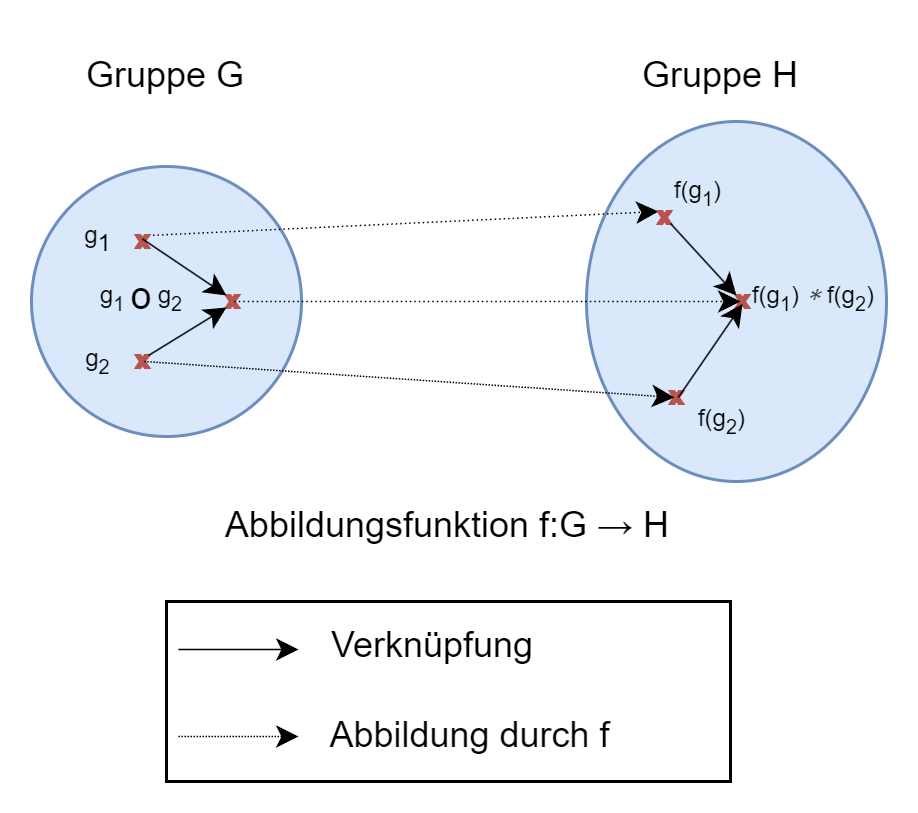
\includegraphics[width=12cm]{figures/group_homomophismus.png}
    \caption{Gruppenhomomorphismus nach \cite{P-98}}
    \label{fig:group_homomorphismus}
\end{figure} 

Bei der homomorphen Verschlüsselung, handelt es sich um einen Gruppenhomomorphismus zwischen der Gruppe der Klartexte $(P,\circ)$ und der Gruppe der Geheimtexte $(C,\ast)$. 
Die Abbildfunktionen sind dabei der Verschlüsselungsalgorithmus $Enc_k:P\to C$ und der Entschlüsselungsalgorithmus $Dec_k:C\to P$ mit einem Schlüssel $k \in K$ \cite{P-98}. 
Daraus lässt sich ableiten, dass folgende Bedingungen erfüllt sind:
\begin{equation*}
    Enc_k(p_1 \circ p_2) = Enc_k(p_1) \ast Enc_k(p_2) 
\end{equation*}
\begin{equation*}
Dec_k(c_1 \ast c_2) = Dec_k(c_1) \circ Dec_k(c_2)
\end{equation*}
Abbildung \ref{fig:homo_enc} zeigt, wie besagter Homomorphismus aussieht.


\begin{figure}[!htb]
    \centering
    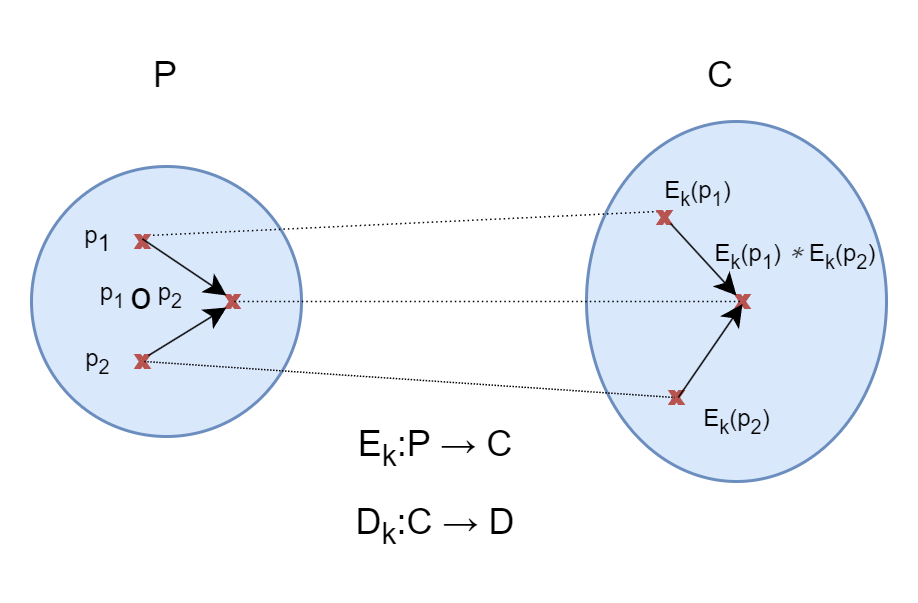
\includegraphics[width=12cm]{figures/homo_enc.png}
    \caption{Homomorphe Verschlüsselung}
    \label{fig:homo_enc}
\end{figure} 

Homomorphe Verschlüsselungen lassen sich dabei in 3 Kategorien einteilen, je nachdem welche Verknüpfungen innerhalb der Gruppen möglich sind \cite{P-42}:
\begin{compactitem}
\item \textbf{Teilweise homomorphe Verschlüsselung (partially):} Entweder Multiplikation oder Addition möglich, jedoch nicht beides.
\item \textbf{Eingeschränkte homomorphe Verschlüsselung (somewhat oder leveled):} Sowohl Multiplikation als auch Addition möglich, jedoch beschränkt durch die Anzahl an durchführbaren Berechnungen. 
\item \textbf{Vollständige homomorphe Verschlüsselung (fully):} Multiplikation und Addition für eine unbegrenzte Anzahl an Berechnungen möglich
\end{compactitem}

Gentry \cite{P-40} stellte 2009 das erste vollständig homomorphe Verschlüsselungssystem vor.
Dabei nutzte er eine eingeschränkt homomorphe Verschlüsselung, welche auf mathematischen Gittern basiert.
Das System war eingeschränkt homomorph, da die Verschlüsselung auf einem Rauschen basierte, welches mit jeder Operation größer wurde und letztendlich nicht mehr für eine korrekte Entschlüsselung sorgte.
Er erweiterte das System mit einer Technik namens Bootstrapping.
Dabei wird der Geheimtext ein zweites Mal verschlüsselt, sodass dieser doppelt verschlüsselt ist.
Anschließend kann mittels des verschlüsselten Schlüssels die ursprüngliche Verschlüsselung homomorph herausgerechnet werden. 
Dadurch wird das Rauschen des Verschlüsselungssystems zurückgesetzt und eine weitere Berechnung ist möglich. 
Kann das ursprünglich eingeschränkte homomorphe Verschlüsselungssystem die homomorphe Entschlüsselung und eine weitere Operation durchführen, dann kann es mittels Bootstrapping zu einem vollständig homomorphen Verschlüsselungssystem umgewandelt werden.
So nutzen beispielsweise Van Dijk et al. \cite{P-100} diesen Fakt aus, und ersetzten die auf Gittern basierte Verschlüsselung durch eine auf Ganzzahlen basierte, eingeschränkt homomorphe Verschlüsselung aus. 

Brakerski und Vaikuntanathan \cite{P-101} verbesserten die Effizienz des bereits geschilderten Ansatzes.
Sie nutzen eine eingeschränkte homomorphe Verschlüsselung auf Basis des Lernen mit Fehlern Problems (Learning with errors) zusätzlich zu einem Relinearisierungsschritt.
Dieser zusätzliche Relinearisierungsschritt reduziert die Größe des Geheimtextes, wodurch die homomorphe Entschlüsselung beim Bootstrapping vereinfacht wird.

Gentry et al. \cite{P-102} stellten eine weitere vollständig homomorphe Verschlüsselung auf Basis des Lernen mit Fehlern Problems vor.
Die darin eingesetzte, eingeschränkt homomorphe Verschlüsselung stellt den Geheimtext als eine Matrix dar.
Die Dimension der Matrix bleibt bei jeder homomorphen Operation gleich und wächst dadurch nicht.
Dies ermöglicht, den Relinearisierungsschritt zu entfernen.
Bei dem Bootstrapping bisheriger Algorithmen, musste der verschlüsselte Schlüssel oder der Public Key des Nutzers mitgeschickt werden.
Bei diesem Ansatz ist es jedoch möglich, alleine mit dem Geheimtext Operationen durchzuführen, die anschließend nur der Nutzer entschlüsseln kann.


Theoretisch wäre das Training eines Neuronalen Netzes mittels vollständiger homomorpher Verschlüsselung möglich, jedoch ist es nicht praktikabel. 
Das Training besteht aus vielen Berechnungsschritten (Inferenze, Berechnen der Verlustfunktion, Gradientenberechnung, Anpassen der Gewichte), welche mit der Größe des Neuronalen Netzes ansteigt.
So wird bereits bei einem Neuronales Netz mit 7 Schichten, Faltungsschichten und vollständig verbundene Schichten, die Trainingszeit auf einer gewöhnlichen CPU, von ungefähr einer Stunde auf ein ganzes Jahr erhöht \cite{P-103}.
Eine Alternative ist es, keine vollständige sondern nur eingeschränkte homomorphe Verschlüsselung zu nutzen.
Takabi et al. \cite{P-104} zeigen wie dies möglich ist.
Um das Problem der begrenzten Anzahl an Berechnungen von eingeschränkter homomorphen Verschlüsselung zu umgehen, wird ein zusätzlicher Schritt eingeführt. 
Wird das Rauschen der Verschlüsselung zu groß und überschreitet einen festgelegten Schwellenwert, muss der aktuelle Zustand entschlüsselt und neu verschlüsselt werden.
Hierdurch wird das Rauschen zurückgesetzt, ohne dass Bootstrapping nötig ist.
Dadurch, dass kein vollständig homomorphes Verschlüsselungssytem genutzt werden muss, können performantere, teilweise homomorphe Verschlüsselungssyteme genutzt werden.

Neben dem Training eines Modells, gibt es eine Vielzahl an Techniken, die Homomorphe Verschlüsselung nur bei der Inferenz der Neuronalen Netze nutzt. 
Diese werden in Kapitel \ref{sec:krypto_inferenz} genauer beschrieben.
Alternativ kann Homomorphe Verschlüsselung beim Verteilten Lernen eingesetzt werden, was in Kapitel \ref{sec:verteiltes_lernen} beleuchtet wird. 





\subsection{Funktionale Verschlüsselung}\label{sec:funktionale_verschlüsselung}

Eine weitere Methodik, Berechnungen auf verschlüsselten Daten durchzuführen, ist die sogenannte Funktionale Verschlüsselung.
Diese wurde 2011 von Boneh et al.\cite{P-44} vorgestellt.
Funktionale Verschlüsselung erlaubt es, eine Funktion $f$ eines Klartextes zu berechnen, wobei nur der Geheimtext als Input der Funktion genutzt wird.
Dies geschieht in vier Schritten\cite{P-44}:
\begin{compactenum}
    \item \textbf{Setup: } In einem Vorbereitungsschritt wird ein Public Key $pk$ und ein Master Secret Key $msk$ erzeugt.
    \begin{equation*}
        (pk, msk) \xleftarrow{} Setup
    \end{equation*}
    \item \textbf{Schlüsselgenerierung: } Der Master Secret Key kann nun genutzt werden, um einen spezifischen Secret Key $sk$ für eine definierte Funktion $f$ zu erzeugen.
    \begin{equation*}
        sk \xleftarrow{} Keygen(msk, f)
    \end{equation*}
    \item \textbf{Verschlüsselung: } Der Public Key $pk$ wird genutzt, um den Klartext $x$, auf welchem die Berechnung durchgeführt werden soll, zu verschlüsseln.
    \begin{equation*}
        c \xleftarrow{} Enc(pk,x)
    \end{equation*}
    \item \textbf{Entschlüsselung: } Die Entschlüsselung des Geheimtextes $c$ mittels des spezifischen Secret Key $sk$ entspricht hierbei der Berechnung der Funktion $f$ mit dem Parameter $x$.
    \begin{equation*}
        f(x) \xleftarrow{} Dec(sk,c)
    \end{equation*}
\end{compactenum}

Die ersten Ansätze um Funktionale Verschlüsselung und Neuronalen Netze zu verbinden, fokussierten sich auf die Inferenz der Modelle, welche in Kapitel \ref{sec:krypto_inferenz} genauer betrachtet werden.
Ein Framework für das Training des Modells mit dem Namen CryptoNN wurde jedoch von Xu et al. \cite{P-53} vorgestellt.
Dieses ermöglicht, ein Modell auf einem fremden Server (Cloud) zu trainieren, ohne dass der Provider Einblick in die Daten erhält.
Dabei wird eine Funktionale Verschlüsselung genutzt, welche die Berechnung des Skalarprodukts und zusätzlich auch die Grundrechenarten (Addition, Subtraktion, Multiplikation und Division) von zwei Vektoren elementweise ermöglicht.
Kombiniert ermöglicht dies, alle notwendigen Berechnungen beim Training des Modells durchzuführen.
CryptoNN führt dabei 3 Rollen ein: Autorität, Client und Server. 
Dabei ist es auch möglich, dass es mehrere Clients gibt, die zusammen ein Modell trainieren.
Gibt es jedoch nur einen Client, so übernimmt dieser auch die Rolle der Autorität.
Die Autorität ist dafür zuständig, einen Master Secret Key $msk$ und einen Public Key $pk$ zu erzeugen, den Public Key $pk$ an den Client zu verteilen und bei Bedarf spezifische Secret Keys $sk_n$ zu erzeugen und an den Server weiterzugeben.
Der Client ist Besitzer der Daten und verschlüsselt diese vor der Übergabe an den Server mit dem Public Key $pk$. 
Der Server führt das tatsächliche Training des Modells durch.
Beim Feedforward Schritt wird Funktionale Verschlüsselung zur Berechnung der Neuronen der ersten Hidden Layer genutzt.
Dafür fordert der Server einen spezifischen Secret Key $sk_n$ an, der die Berechnung der ersten Schicht ermöglicht.
Der restliche Feedforward Schritt erfolgt unverschlüsselt.
Wenn der Client auch das Label verschlüsselt, kann die Berechnung der Verlustfunktion für jedes Output Neuron ebenfalls verschlüsselt erfolgen.
Abbildung \ref{fig:cryptonn} zeigt das CryptoNN Framework.

\begin{figure}[!htb]
    \centering
    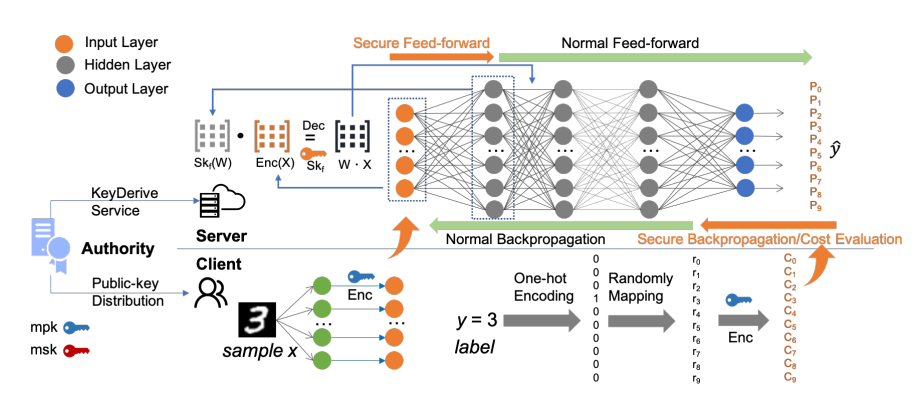
\includegraphics[width=15cm]{figures/cryptoNN}
    \caption{CryptoNN Framework \cite{P-53}}
    \label{fig:cryptonn}
\end{figure} 

Ein Problem des CryptoNN Frameworks ist jedoch, dass davon ausgegangen wird, dass der Server kein Angreifer ist, der effektiv versucht Daten zu extrahieren.
Ansonsten könnte dies dazu führen, dass der Server diverse White-Box Angriffe (Kapitel \ref{sec:angriffe}) durchführen könnte, da das Modell unverschlüsselt vorliegt.
Die Methodik ist demnach darauf ausgelegt dafür zu sorgen, dass Clients Daten verschlüsselt übertragen können und diese nicht beispielsweise von dem Cloud Provider mitgelesen werden können.


\subsection{Verteiltes Lernen}\label{sec:verteiltes_lernen}

Das Verteilte Lernen bietet einige besondere Herausforderungen, die bereits in Kapitel \ref{sec:angriffe_verteiltes_lernen} betrachtet wurden. 
Einige bereits beschriebene Methoden lassen sich problemlos auf das Verteilte Lernen anwenden.
Sollen beispielsweise die Daten der einzelnen Teilnehmer geteilt werden, so ist es möglich, diese mit den Methoden aus Kapitel \ref{sec:aufbereitung_datensatz} vorzuverarbeiten.
Jedoch gibt es auch spezielle Methoden, die auf das Verteilte Lernen ausgerichtet sind.
Im Folgenden werden einige davon genauer beschrieben.

\subsubsection*{Distributed Selective SGD}
Shokri und Shmatikov \cite{P-78} stellen eine Methode vor, bei welcher mehrere Teilnehmer gleichzeitig ein Modell trainieren, ohne dabei die Daten untereinander zu teilen.
Diese wird Distributed Selective Stochastic Gradient Descent oder auch Distributed Selective SGD genannt.
Das Modell liegt dabei auf einem zentralen Server.
Bei der ersten Iteration laden die Teilnehmer das gesamte Modell herunter, bei weiteren Iterationen nur eine festgelegte Anzahl der am meisten geupdateten Parametern (Gewichte).
Dadurch soll vermieden werden, dass Overfitting auf den Daten eines einzelnen Teilnehmers auftritt.
Die heruntergeladenen Parameter ersetzen die alten Parameter an der entsprechenden Stelle im lokalen Modell.
Anschließend wird dieses lokale Modell mit den eigenen Daten trainiert und im Nachhinein eine festgelegte Menge an Gradienten übertragen. 
Diese können dabei entweder randomisiert ausgewählt werden, oder möglichst nach Größe sortiert werden.
Alle Teilnehmer wählen die zu teilenden Gradienten mit der gleichen Strategie aus und behalten diese über den Trainingsprozess bei.
Zusätzlich ist es möglich, die Gradienten vor dem Teilen noch mit in der Größe zu begrenzen oder Rauschen mittels Differential Privacy hinzuzufügen.
Abbildung \ref{fig:dssgd} zeigt die Architektur von Distributed Selective SGD.

\begin{figure}[!htb]
    \centering
    \includegraphics[width=12cm]{figures/dssgd}
    \caption{Distributed Selective SGD \cite{P-78}}
    \label{fig:dssgd}
\end{figure} 

Durch das eingeschränkte Teilen der Gradienten werden so wenig Information wie nötig geteilt, jedoch ist die Güte des Modells kaum schlechter als bei normalem Training.
Die Autoren begründen dies damit, dass das lokale Modell lokale Minima durch das Ersetzen von Parametern aus dem geteilten Modell verlassen kann und so weiter eher Richtung globales Minimum konvergiert. 
Zwei Parameter steuern dabei die Performance des Modells beim Training mit Distributed Selective SGD: das Privacy Budget $\epsilon$ und die Anzahl der zu teilenden Gradienten.
Werden mehr Gradienten nach jedem Schritt von jedem Teilnehmer geteilt, kann das Privacy Budget $\epsilon$ niedriger angesetzt werden, um dennoch eine nahezu identische Güte im Vergleich zu einem normal trainierten Modell zu erhalten.

\subsubsection*{Anspruchsvolle kryptografische Methoden}

Takabi et al. \cite{P-104} nutzen Homomorphe Verschlüsselung, um ein Modell zu trainieren, welches Daten von mehreren Teilnehmern nutzen kann. 
Die Funktionsweise der Methode mit einem Teilnehmer wurde bereits in Kapitel \ref{sec:homomorphe_verschlüsselung} beschrieben.
Diese lässt sich problemlos auf mehrere Teilnehmer erweitern, indem abwechselnd Daten jedes Teilnehmers verschlüsselt an den Server übertragen wird und diese für das Training des Modells mittels Homomorpher Verschlüsselung genutzt wird.
Da Daten jeweils verschlüsselt sind, ist es nicht möglich, Daten anderer Teilnehmer zu extrahieren.

Auch das auf Funktionaler Verschlüsselung basierende Framework CryptoNN \cite{P-53}, welches in Kapitel \ref{sec:funktionale_verschlüsselung} vorgestellt wurde, kann für Verteiltes Lernen genutzt werden. 
Die Rolle des Clients können dabei mehrere Teilnehmer übernehmen, wohingegen die Autorität jedoch von einem separaten System übernommen werden muss. 
Anschließend können auch bei dieser Methode abwechselnd Daten von verschiedenen Teilnehmern zum Trainieren genutzt werden.

Ein weiterer Ansatz für Verteiltes Lernen, welches auf Funktionaler Verschlüsselung basiert, wurde von Xu et al. \cite{P-33} mit dem Namen HybridAlpha vorgestellt.
Ähnlich zu dem bereits beschriebenen CryptoNN Framework, gibt es auch eine Autorität, welche die benötigten kryptografischen Schlüssel an die Server und Clients verteilt.
Jedoch übertragen die Clients keine Daten an den Server, sondern trainieren ein lokales Modell.
Die aktualisierten Modellparameter werden anschließend mit Differential Privacy verrauscht und dann verschlüsselt an den Server übertragen.
Hat der Server alle verschlüsselten Modellparameter jedes Teilnehmers gesammelt, wird mittels Funktionaler Verschlüsselung die Summe der Gewichte jedes Neurons gebildet.
Daraus kann der Server anhand der Anzahl an Teilnehmern, den Durchschnittswert für jedes Gewicht jedes Neurons bilden und aktualisiert damit das globale Modell.
Die Autoren zeigen anhand des MNIST Datensatze \cite{D-MNIST}, dass die Güte eines Modells, welches mit HyrbidAlpha ohne Differential Privacy trainiert wurde, sehr nahe der Güte eines Modells ist, welches in einem Verteilten Lernen Szenario ohne HyrbidAlpha gelernt wurde. 
Wird jedoch zusätzlich Differential Privacy genutzt, sinkt die Güte des Modells. 
Mit einem Privacy Budget von $\epsilon=0,5$ sinkt die Genauigkeit der Klassifikation um knapp 10\%.


\subsubsection*{Secure Multi-Party Computation}

Bei der Secure Multi-Party Computation handelt es sich um einen Forschungsbereich mit dem Ziel, dass Teilnehmer gemeinsam eine Funktion berechnen können, ohne dass die einzelnen Eingabewerte aufgedeckt werden. 
Methoden dieses kryptografischen Forschungsgebiets können auch für Neuronale Netze genutzt werden.

Rouhani et al. \cite{P-71} stellten ein Framework namens DeepSecure vor, welches Oblivious Transfer, zu Deutsch vergessliche Übertragung, und Garbled Circuits, zu Deutsch verdrehte Schaltkreise, nutzt.
Oblivious Transfer ist ein kryptografisches Protokoll zwischen einem Sender und einem Empfänger, bei dem der Empfänger einen Index zwischen 1 und $n$ auswählt und der Sender die Nachricht mit dem entsprechenden Index übermittelt. 
Der Sender weiß dabei jedoch nicht, welcher Index ausgewählt wurde.
Diese Methodik wird auch 1-aus-$n$ Oblivious Transfer genannt.
Garbled Circuits, auch Yao's Garbled Circuits genannt, ist ebenfalls ein Protokoll, bei der eine Funktion als Boolescher Schaltkreis mit zwei Eingabegattern dargestellt wird.
Dabei erstellt einer der beiden Teilnehmer, hier Alice genannt, Wahrheitstabellen zu jedem Logikgatter des Schaltkreises. 
Die Inputs sind dabei nicht 0 und 1, sondern jeweils eine Folge von $k$ randomisierten Bits, welche 0 und 1 kodieren.
Die Ergebnisspalte dieser Wahrheitstabellen verschlüsselt Alice anschließend mit den beiden Inputs, sodass dies nur mit den beiden Inputs wieder entschlüsselt werden kann. 
Zusätzlich wird die Reihenfolge der Zeilen randomisiert, damit aufgrund der Reihenfolge keine Rückschlüsse gewonnen werden können. 
Dieser Schritt wird Garbling genannt und die entstandenen Tabellen sind sogenannte Garbled Tabellen.
Anschließend überträgt Alice die Garbled Tabellen an den zweiten Teilnehmer, hier Bob.
Mittels 1-aus-2 Oblivious Transfer wählt Bob eine von zwei Nachrichten aus, wobei der Index seinem Input entspricht und die zwei Nachrichten die kodierten Labels von Alice sind.
Die erhaltene Nachricht und das eigene Label können nun genutzt werden, um die Ergebnisspalte einer Garbled Tabelle zu entschlüsseln.
Bob führt dies für jedes Gatter des Schaltkreises aus.
Am Ende erhält Bob den Output des letzten Gatters, welchen jedoch einer der randomisierten Bitfolgen ist. 
Er übermittelt diesen an Alice und erhält dadurch den entsprechenden 0 oder 1 Wert.
DeepSecure wendet Garbled Circuits auf Neuronale Netze an.
Alice würde in diesem Fall die Daten besitzen und Bob das Modell, welches trainiert wird.
Der Feedforward Schritt würde dabei durch einen Booleschen Schaltkreis aus XOR und XNOR Gattern implementiert werden, wodurch die Berechnung der Vorhersage erfolgt.
Dadurch kann Bob den Wert der Verlustfunktion und anschließend der Gradienten bestimmen, ohne die Daten von Alice zu kennen.
Alice würde jedoch auch nicht die genauen Gewichte des Modells kennen.
Allerdings ist die Anzahl an benötigten Gattern, um ein Neuronales Netz darzustellen, enorm.
Einige Operationen, wie die Anwendung einer Aktivierungsfunktion, benötigt mehrere tausende Gatter.
Jedes dieser Gatter sorgt ebenfalls dafür, dass eine Menge an Daten übertragen werden muss.
Ein Neuronales Netz, welches $28\times28$ Pixel Bilder als Input nimmt, zwei Hidden Layers mit 300 und 100 Knoten (Sigmoid Aktivierungsfunktion) besitzt und eine Softmax Output Layer mit 10 Knoten hat, würde circa 171.300.000 Gatter ausmachen und in einem Feedforward Schritt ungefähr 2 Gigabyte an Daten übertragen.

\subsubsection*{Aggregation}
Eine alternative Methode wird von Bonawitz et al. \cite{P-36} vorgestellt.
Diese basiert auf sicherer Aggregation, welche mehrere Daten von unterschiedlichen Teilnehmern verbindet, ohne dass die Daten eines einzelnen Teilnehmers erkenntlich werden.
Teilnehmer trainieren ein lokales Modell mit den eigenen privaten Daten. 
Bevor die angepassten Parameter aber an das globale Modell übertragen werden, werden die Parameter mit den Parametern anderer Teilnehmer kryptografisch aggregiert.
Dadurch erhält das globale Modell Gradienten aller Trainingsdaten, ohne die einzelnen Daten zu kennen.



\section{Betrieb des Modells}\label{sec:betrieb}

Nachdem ein Neuronales Netz trainiert wurde, muss dieses irgendwie für Nutzer zugänglich gemacht werden.
So könnte beispielsweise eine API zur Verfügung stehen, über welches ein Modell auf einem Server erreichbar ist.
Alternativ kann auch das ganze Modell ausgeliefert werden.
Auch hierbei gibt es zusätzlich Möglichkeiten, die Vertraulichkeit der Trainingsdaten zu schützen.

% \subsection{Limitierungen}
% %\subsection{Perturbation}
\subsection{Differential Privacy}\label{sec:dp}

Differential Privacy ist eine Technik, welche 2006 von Cynthia Dwork \cite{P-26} vorgestellt wurde.
Ziel dabei ist es, Zugriff auf eine Datenmenge zu ermöglichen, welche sowohl nützliche Erkenntnisse zulässt, als auch die Privatsphäre eines einzelnen Datensatzes schützt.

Differential Privacy kann dabei an 3 unterschiedlichen Stellen der Machine Learning Pipeline genutzt werden:
\begin{compactitem}
\item \textbf{Verfremdung der Trainingsdaten:} Diese Methodik wird folgend in diesem Kapitel erläutert.
\item \textbf{Trainingsalgorithmus:} Kapitel \ref{sec:dp_training} beschreibt, welche Anpassungen am Trainingsalgorithmus vorgenommen werden können, um Differential Privacy zu gewährleisten.
\item \textbf{Vorhersage des Modells:} Bevor die Vorhersage des Modells weitergeleitet wird, könnte diese verrauscht werden. Kapitel \ref{sec:betrieb} stellt dieses Vorgehen vor.
\end{compactitem}

Differential Privacy \cite{P-26} sorgt dafür, dass ein Mechanismus, auch Abfrage oder Funktion, welche eine Menge an Datensätzen als Eingabe akzeptiert, keinen konstanten Wert mehr zurückgibt.
Stattdessen wird dem Mechanismus zufälliges Rauschen mit einer festgelegten Intensität hinzugefügt.
Der Mechanismus gibt also eine Stichprobe einer Verteilung zurück, bei der das tatsächliche Ergebnis dem Erwartungswert entspricht.
Demnach können eindeutige Feststellungen über Eigenschaften nicht getroffen werden.
Ziel des Verrauschens ist es, dass wenn der Mechanismus auf zwei Datenmengen, die sich in einem Datensatz unterscheiden, ausgeführt wird, die Ergebnisse sich maximal um einen Faktor $e^\epsilon$ unterscheiden. 
Demnach ist der Einfluss eines Datensatzes auf eine Berechnung mit der gesamten Datenmenge quantifizierbar und kann begrenzt werden.
Dabei kann der Wert $\epsilon$, welcher auch Privacy Budget genannt wird, festgelegt werden.

Formal lautet die Definition von $\epsilon$-Differential Privacy wie folgt \cite{P-26}:\\
\textit{
Ein randomisierter Mechanismus $M$, welche eine Menge an Datensätzen $D$ auf einen Wertebereich $R$ abbildet, weist $\epsilon$-Differential Privacy auf, wenn für alle Mengen an Datensätze $D_{1}$ und $D_{2}$ die sich in höchstens einem Datensatz unterscheiden $||D_{1} - D_{2}||_{1} \leq 1$ , gilt:}
\begin{equation}
\resizebox{!}{0.3cm}{$
    P[M(D_{1}) \in R] \leq e^{\epsilon} \times P[M(D_{2}) \in R]
$}
\end{equation}
\textit{$P$ beschreibt dabei die Wahrscheinlichkeit, dass der Erwartungswert gezogen wird.}

Es gibt unterschiedliche Algorithmen, um das Ergebnis eines Mechanismus zu verrauschen.
Diese werden im späteren Verlauf des Kapitels genauer beleuchtet.

Dwork und Roth \cite{P-27} fügten der Definition noch einen Parameter $\delta$ hinzu, welcher erlaubt, dass die Bedingungen von $\epsilon$-Differential Privacy zu einem definierten Grad verletzt werden können.
Der Wert von $\delta$ sollte dabei niedriger sein, als die Inverse der Anzahl an Datensätzen im Datenbestand.
Die damit angepasste Definition von ($\epsilon$,$\delta$)-Differential Privacy lautet \cite{P-27}:\\
%Damit lautet die formale Definition von Differential Privacy wie folgt \cite{P-27}:
\textit{
Ein randomisierter Mechanismus $M$, welche eine Menge an Datensätzen $D$ auf einen Wertebereich $R$ abbildet, erfüllt ($\epsilon$,$\delta$)-Differential Privacy, wenn für alle Mengen an Datensätze $D_{1}$ und $D_{2}$ die sich in höchstens einem Datensatz unterscheiden $||D_{1} - D_{2}||_{1} \leq 1$ , gilt:}
\begin{equation}
\resizebox{!}{0.3cm}{$
    P[M(D_{1}) \in R] \leq e^{\epsilon} \times P[M(D_{2}) \in R] + \delta
$}
\end{equation} 

Konkret sagen die Definitionen aus, dass eine randomisierte Funktion $M$, auf zwei Datenbeständen $D_{1}$ und $D_{2}$ mit maximal einem unterschiedlichen Datensatz $||D_{1} - D_{2}||_{1} \leq 1$, jeweils Stichproben einer Verteilung ausgibt, wobei sich die Verteilungen nur um den Faktor $\epsilon$ und den Summand $\delta$ unterscheiden dürfen.
Dabei bestimmt das Privacy Budget, $\epsilon$ und $\delta$, wie stark sich die Ergebnisse unterscheiden dürfen.
Wie diese beiden Werte konfiguriert werden können, hängt dabei vom Algorithmus des Rauschens ab.

\subsubsection*{Konfiguration des Privacy Budgets}

Der $\delta$-Wert wird oftmals als konstanter Wert festgelegt, wobei dieser kleiner als die Inverse der Anzahl an Datensätzen im Datenbestand sein sollte \cite{P-27}.
Die Wahl von $\epsilon$ ist daher entscheidend. 
Abbildung \ref{fig:dp_privacy_budget} zeigt den Einfluss des $\epsilon$-Werts auf die Nützlichkeit und die Vertraulichkeit von Mechanismen.
Kleine Werte für $\epsilon$, also ein kleines Privacy Budget, bedeutet dabei, dass die Differenz eines Mechanismus durch einen zusätzlichen Datensatz, sich weniger stark verändern kann, was für einen besseren Schutz der Privatsphäre sorgt.
Jedoch wirkt sich dies negativ auf die Nützlichkeit der Abfragen aus, da kleine Privacy Budgets für ein großes Rauschen sorgen, was öfters falsche Ergebnisse liefert.
Dies bedeutet, dass es keinen optimalen Wert für $\epsilon$ gibt, sondern dieser für jeden Use Case mittels einer Abwägung zwischen Sicherheit und Nützlichkeit, neu bestimmt werden muss.
Nutzt ein Modell beispielsweise nur öffentliche, unsensible Daten, ergibt es keinen Sinn einen niedrigen $\epsilon$-Wert festzulegen, da die Vertraulichkeit der Daten nicht entscheidend ist.
Werden jedoch hochsensible Daten genutzt, kann es sein, dass die Sicherheit der Daten wichtiger eingestuft wird, als die Nützlichkeit des Modells. 
Hier empfiehlt sich ein niedriger $\epsilon$-Wert.
Ein $\epsilon$-Wert von Unendlich bedeutet, dass sich die Ergebnisse von Mechanismen um beliebige Werte unterscheiden dürfen, weshalb kein Rauschen notwendig wäre. 
Dies ist bei Mechanismen ohne Differential Privacy bereits der Fall.

\begin{figure}[!htb]
    \centering
    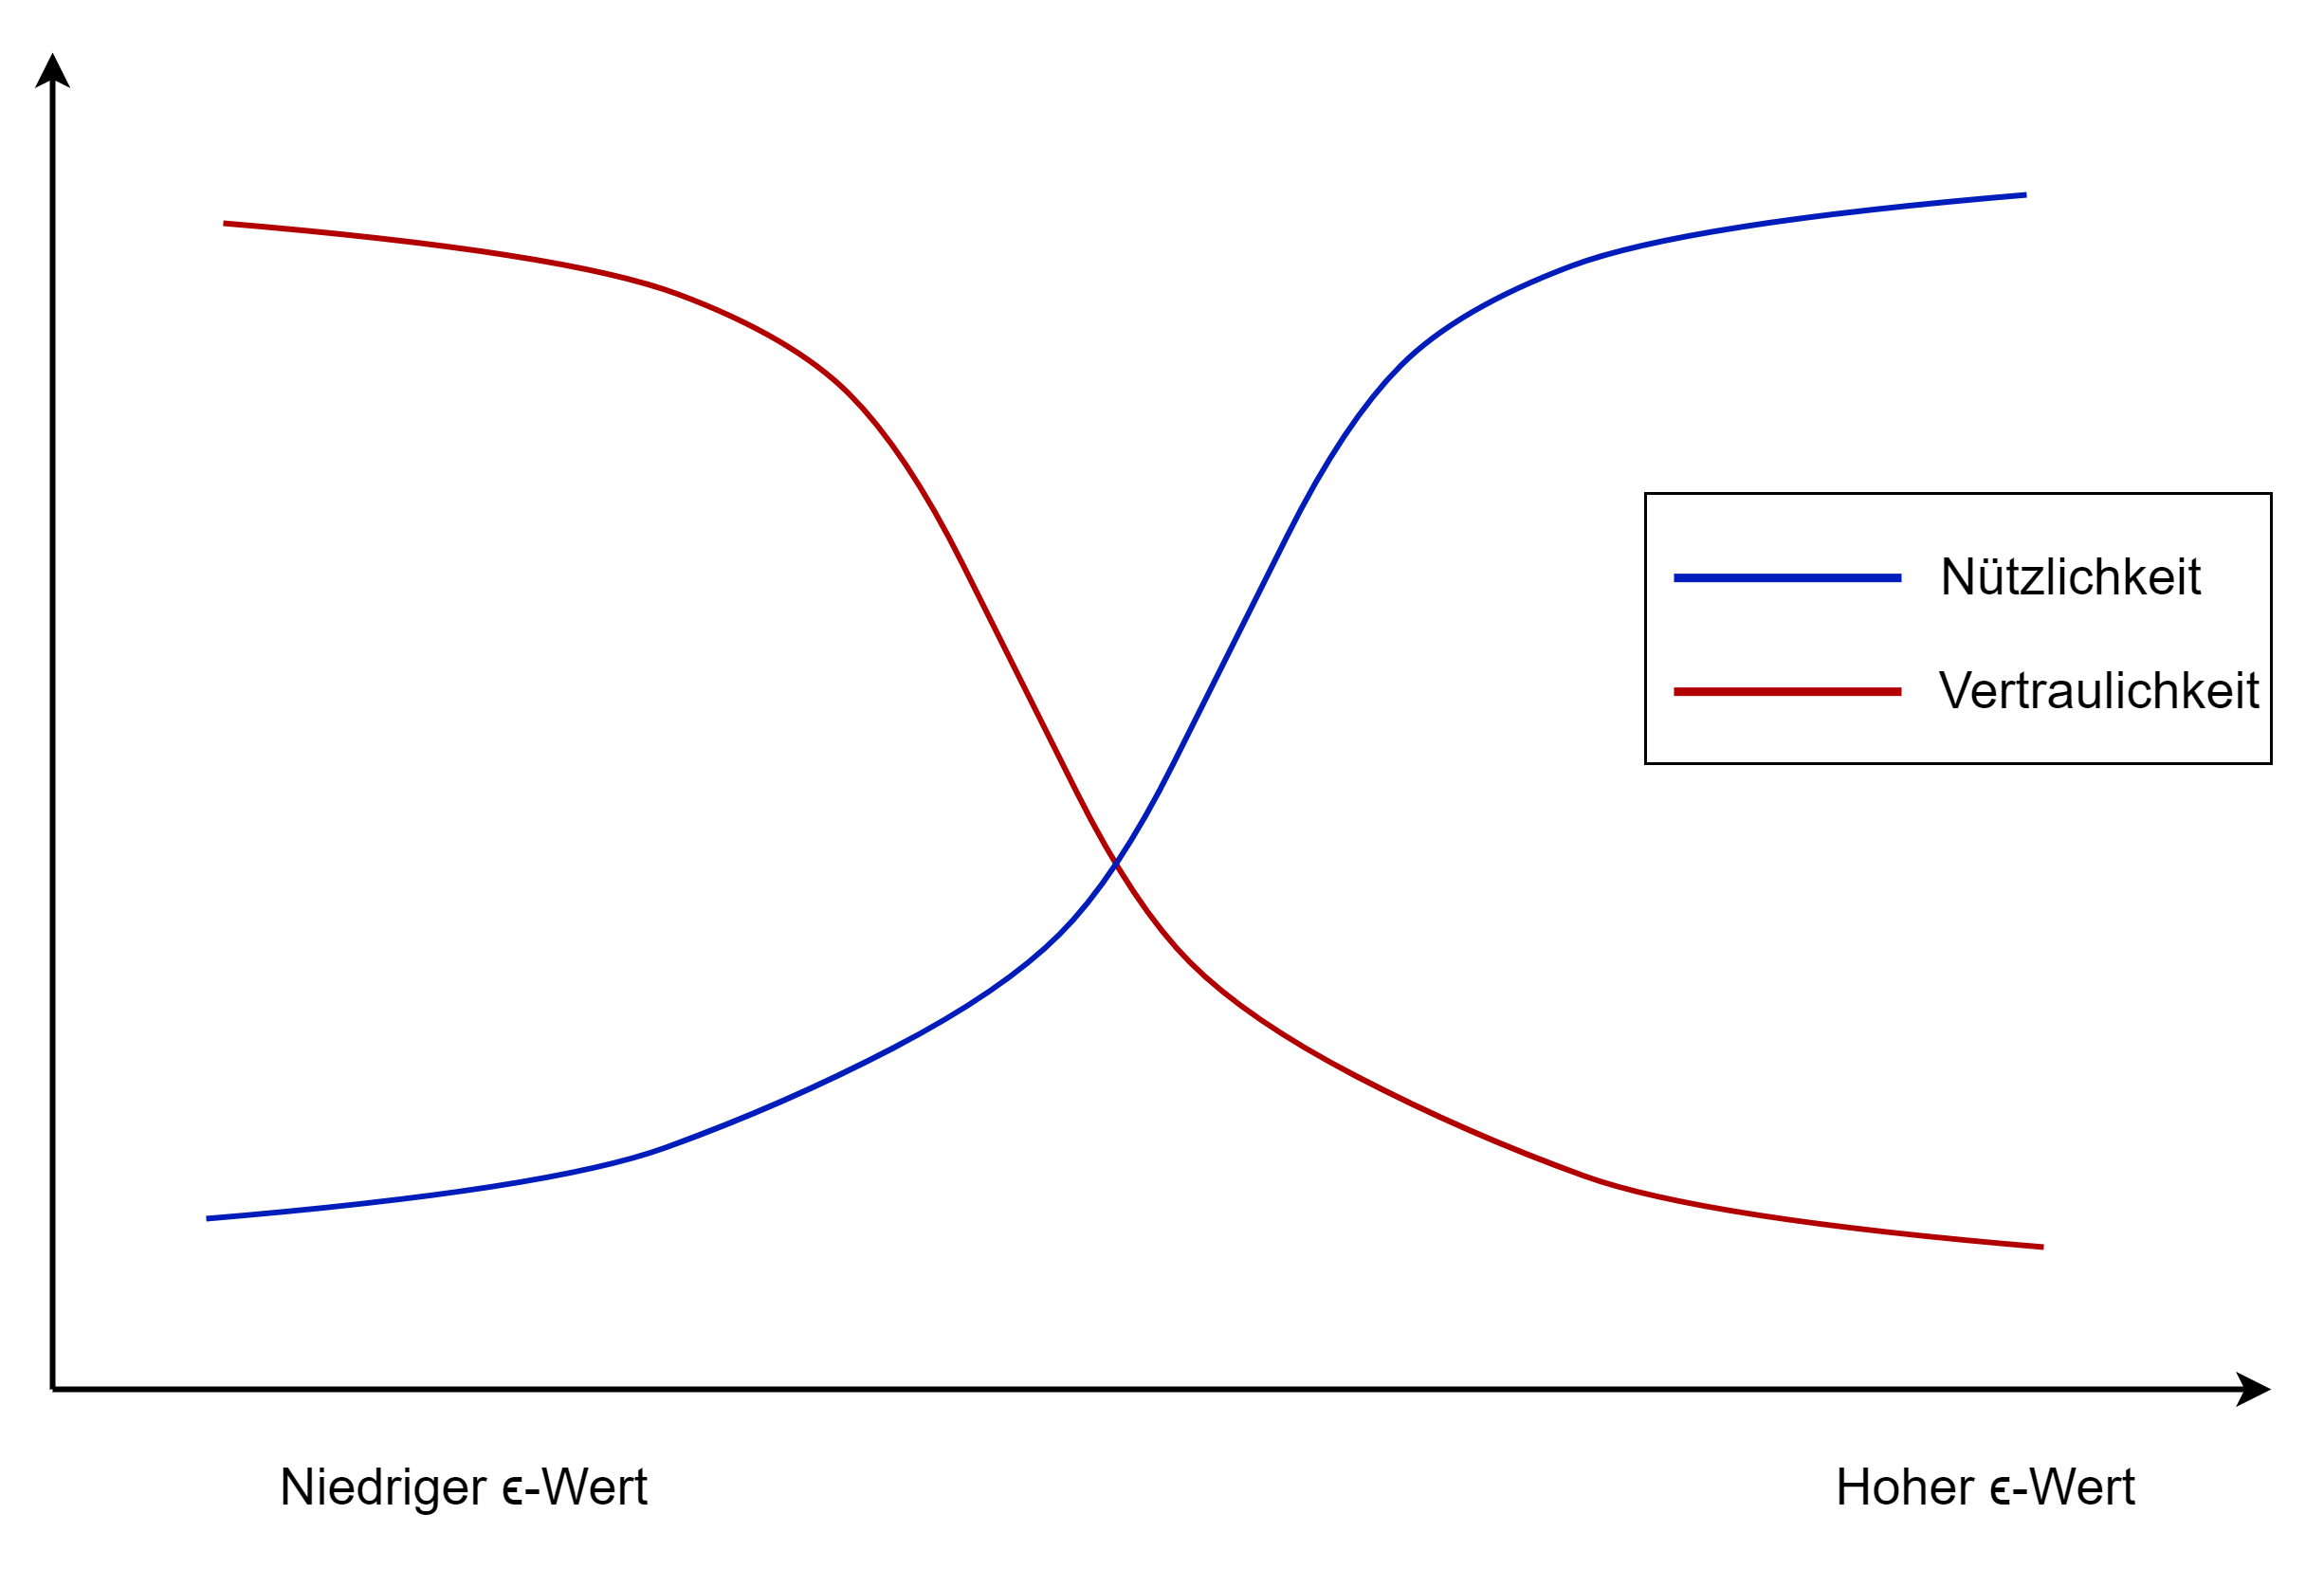
\includegraphics[width=12cm]{figures/dp_privacy_budget.png}
    \caption{Einfluss von $\epsilon$}
    \label{fig:dp_privacy_budget}
\end{figure} 

\subsubsection*{Beispiel für Differential Privacy}

Abbildung \ref{fig:dp} zeigt, wie sich Abfragen mit und ohne Differential Privacy unterscheiden.
Dabei führt ein Angreifer zunächst eine Abfrage über das Durchschnittsgehalt eines Unternehmens auf einem Datenbestand ohne Differential Privacy aus. 
Er erhält hier einen konkreten Wert als Ergebnis.
Anschließend wird der Datenbestand um einen Eintrag erweitert, weil das Unternehmen einen neuen Mitarbeiter hat.
Führt der Angreifer die Abfrage um das Durchschnittsgehalt erneut aus, erhält dieser einen angepassten, neuen Wert.
Dadurch kann er anhand der Anzahl der Mitarbeiter des Unternehmens und der Differenz der beiden Abfragen das exakte Gehalt des neuen Mitarbeiters bestimmen.
Anders sieht dies mit Differential Privacy aus. 
Dabei werden beide Abfragen mit zufälligem Rauschen angereichert. 
Es wird also nur eine Stichprobe einer Verteilung zurückgegeben. 
Bei einer gleichen Abfrage auf den gleichen Datenbestand, können also ebenfalls unterschiedliche Werte zurückgegeben werden.
Führt der Angreifer zwei Abfragen aus, einmal auf dem alten Datenbestand und auf dem Datenbestand mit dem neuen Mitarbeiter, kann er keinen exakten Wert des Gehalts des neuen Mitarbeiters ermitteln.
Differential Privacy bietet einige Algorithmen, wie dieses Rauschen hinzugefügt werden kann, wobei Parameter $\epsilon$ und $\delta$ die Stärke des Rauschens bestimmen und damit auch, wie nah die beiden Ergebnisse aneinander sind.

\begin{figure}[!htb]
    \centering
    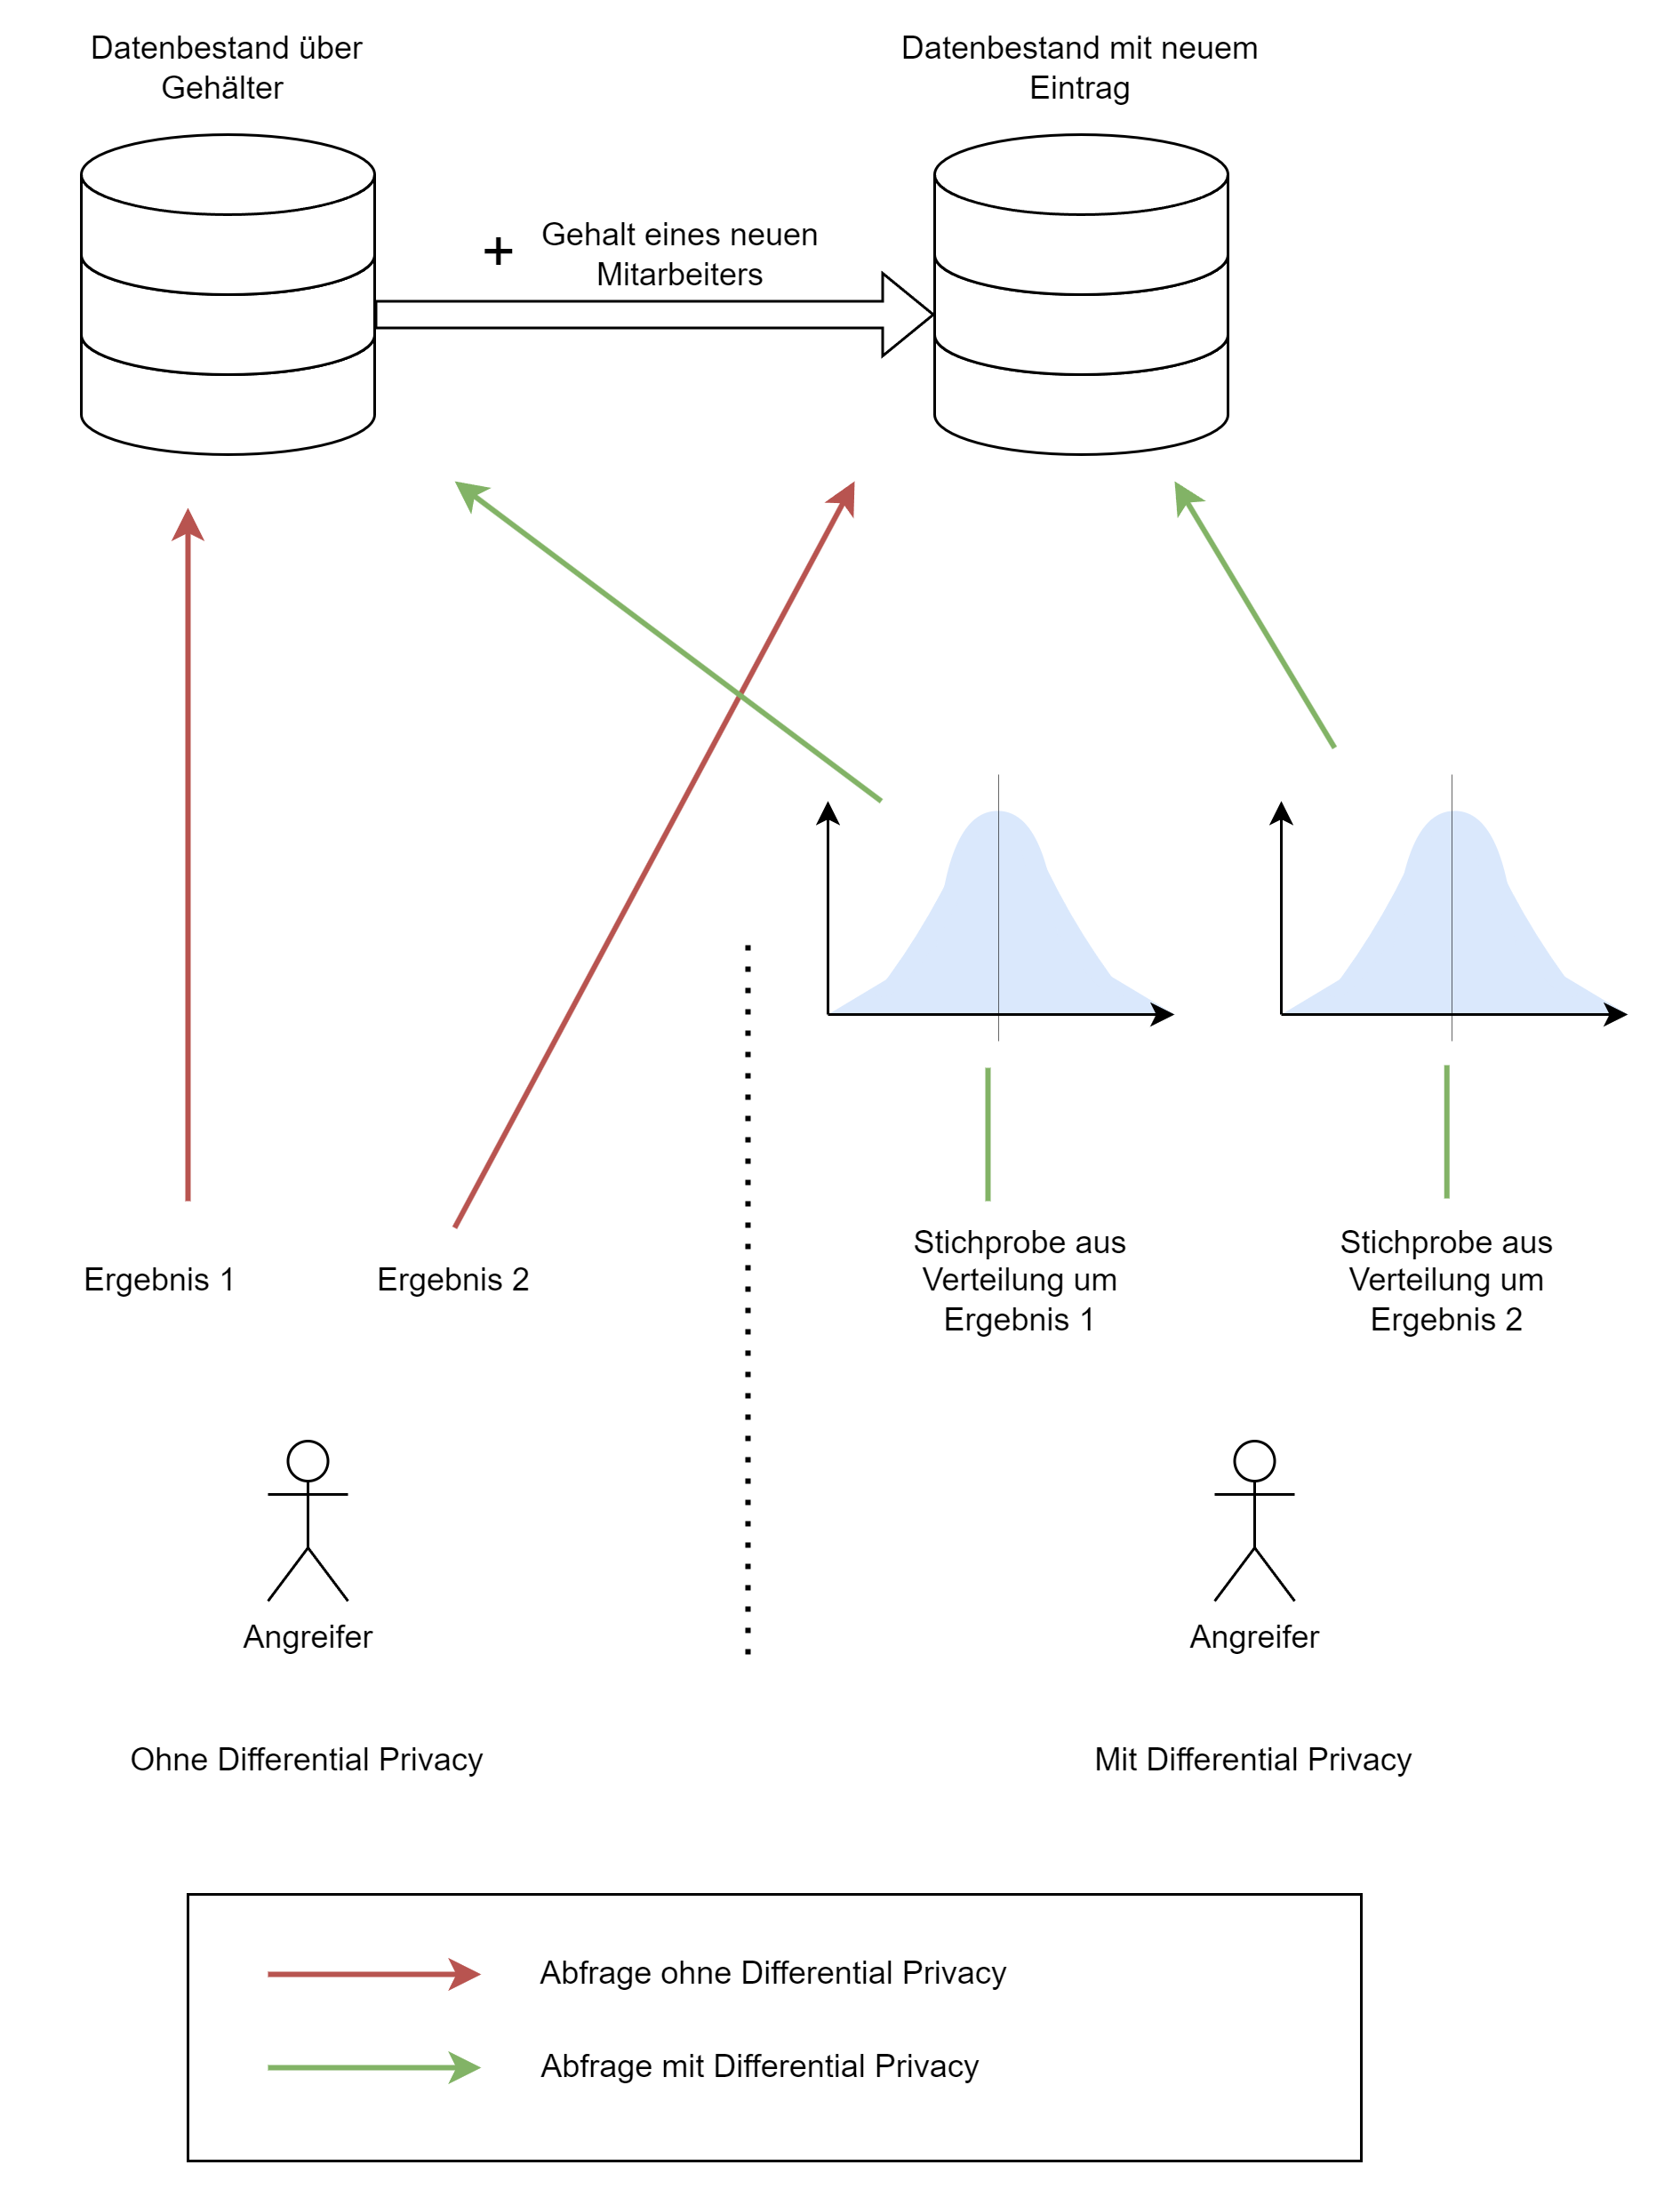
\includegraphics[width=\textwidth]{figures/dp}
    \caption{Beispiel Differential Privacy}
    \label{fig:dp}
\end{figure} 

\subsubsection*{Algorithmen für Differential Privacy}
Die Art des Rauschens, welche über die Ausgabe einer Abfrage gelegt wird, kann unterschiedlichster Herkunft sein.
Dwork und Roth \cite{P-27} stellen eine ganze Reihe dieser Mechanismen vor, die im Folgenden beschrieben werden.

Bei der Technik der randomisierten Antwort, im Englischen Random Response, wird mit einer festgelegten Wahrscheinlichkeit, ein falsches Ergebnis ausgegeben. 
Dies entspricht dem Rauschen dieser Methode.
Wird beispielsweise eine Person gefragt, ob sie eine gewisse Aktivität durchgeführt hat, wird mit 25-prozentiger Wahrscheinlichkeit die falsche Antwort selektiert.
Ist die Wahrheit \textit{\dq Ja\dq}, dann gilt $P[Antwort = \dq Ja\dq \mid Wahrheit = \dq Ja\dq] = 3/4$ und $P[Antwort = \dq Nein\dq \mid Wahrheit = \dq Ja\dq]$.
Gleiches gilt, wenn die Wahrheit \textit{\dq Nein\dq} wäre.
Die jeweils ausgegebene Antwort kann dadurch glaubhaft abgestritten werden.
\begin{equation} \label{formula:random_response}
\begin{split}
\frac{P[Antwort = \dq Ja\dq \mid Wahrheit = \dq Ja\dq]}{P[Antwort = \dq Ja\dq \mid Wahrheit = \dq Nein\dq]} = \frac{3/4}{1/4} = \\
\frac{P[Antwort = \dq Nein\dq \mid Wahrheit = \dq Nein\dq]}{P[Antwort = \dq Nein\dq \mid Wahrheit = \dq Ja\dq]} =  3
\end{split}
\end{equation}

Formel \ref{formula:random_response} zeigt, dass eine Antwort, egal ob diese \textit{\dq Ja\dq} oder \textit{\dq Nein\dq} lautet, mit einem Verhältnis von 3 abgestritten werden kann.
Der Faktor, um den sich die Wahrscheinlichkeit einer Antwort unterscheidet, wenn sich die Wahrheit ändert, liegt demnach auch bei 3.
Daraus resultiert, dass die Technik der randomisierten Antwort, mit einer 25-prozentigen Wahrscheinlichkeit einer falschen Antwort, eine ($ln 3$, 0)-Differential Privacy unterstützt.
Der natürliche Logarithmus $ln$ muss hier genutzt werden, da die Definition von Differential Privacy die Exponentialfunktion als Faktor betrachtet. 
Demnach erhält man durch $\epsilon = ln 3$ einen Unterschied um den Faktor $e^{ln 3} = 3$.

Eine weitere Technik für Differential Privacy ist der Laplace-Mechanismus.
Dabei wird das Rauschen, welches über das Ergebnis der Abfrage gelegt wird, aus einer Laplace-Verteilung ermittelt.
Eine Bedingung ist dabei, dass es sich bei dem Ergebnis der Abfrage um einen Zahlenwert handelt.
Die Dichtefunktion der Laplace-Verteilung, zentriert um den Erwartungswert $\mu=0$, mit dem Skalenparameter $\sigma$, lautet \cite{P-27}:
\begin{equation}
\resizebox{!}{0.55cm}{$
    Lap(x|\sigma) = \frac{1}{2\sigma}\times e^{(-\frac{|x|}{\sigma})}
$}
\end{equation}
wobei $\sigma$ die Steigung der Funktion beeinflusst.
Um nun ein geeignetes $\sigma$ zu wählen, muss zuerst ein Wert ermittelt werden, um den sich eine Funktion bei Änderung eines Datenpunktes maximal unterscheiden kann.
Diese sogenannte Sensitivität wird als $\Delta f$ notiert.
Geht es beispielsweise um eine Anzahl an Datensätzen, so würde ein neuer Datensatz die Anzahl um den Wert 1 erhöhen.
Folglich ist $\Delta f = 1$, denn die Anzahl wird sich durch einen neuen Datensatz um den Wert 1 verändern.
Es gibt jedoch auch Fälle, in denen der Wert der Sensitivität nicht eindeutig ist, beispielsweise bei dem obigen Gehaltsbeispiel.
Das Gehalt einer neuen Person könnte für eine beliebige Veränderung des Durchschnittsgehalts sorgen, da theoretisch jedes Gehalt möglich wäre.
Realistisch betrachtet gibt es jedoch einen Wertebereich, in dem sich alle Gehälter befinden. 
Dieser könnte beispielsweise von 0 Euro bis 10 Milliarden Euro reichen. 
Jedoch sollten die Grenzen möglichst nahe an den echten Grenzen liegen. 
10 Milliarden Euro ist theoretisch möglich, jedoch ist eine Grenze von 200.000 Euro realistischer.
Dieser Wertebereich muss also fachlich festgelegt werden.
In diesem Beispiel wäre die Sensitivität $200.000/n$, wobei $n$ die Anzahl der Mitarbeiter ist.


Um ($\epsilon$,0)-Differential Privacy zu erreichen, muss die Ausgabe einer Abfrage $M$ mit zufälligen Werte der Laplace-Verteilung $Lap(x | \Delta f/\epsilon)$ verrauscht werden \cite{P-27}: 
\begin{equation}
    M(D) = f(D) + (Y_1, ... Y_k),\text{ mit } Y_i \sim Lap(x| \Delta f/\epsilon)
\end{equation}


Eine Abwandlung des Laplace-Mechanismus ist es, anstatt der Laplace-Verteilung, eine Gaußverteilung zu nutzen. Die Dichtefunktion dieser zentriert um den Erwartungswert $\mu=0$ lautet \cite{P-27}:
\begin{equation}\label{formula:gauß}
\resizebox{!}{0.55cm}{$
    Gau\text{\textit{ß}}(x|\sigma) = \frac{1}{\sigma\sqrt{2\pi}}\times e^{-\frac{1}{2}(\frac{x}{\sigma})^2}
$}
\end{equation}
Der Gauß-Mechanismus liefert ($\epsilon$,$\delta$)-Differential Privacy, wenn $\sigma = \Delta f \frac{\text{ln}(1/\delta)}{\epsilon}$ ist \cite{P-27}.

Neben den bereits beschriebenen Mechanismen gibt es noch den Exponential-Mechanismus. 
Bei diesem wird ein Element aus einer Menge ausgegeben, welches anhand einer Bewertungsfunktion ausgewählt wird.
Die Abfrage an einen Datenbestand liefert also keine Zahl, sondern einen Datensatz oder Attributwert aus diesem.
Der Exponential-Mechanismus benötigt eine Bewertungsfunktion $u:D x R \xrightarrow{} \mathbb{R}$, welche für jede potenzielle Ausgabeoption $R$ aus einer Menge an Datensätzen $D$, einen Nutzwert im Wertebereich $\mathbb{R}$ berechnet.
Als Sensitivität $\Delta f$ entspricht der Sensitivität der Bewertungsfunktion $\Delta f = \Delta u$
Die Anfrage erfüllt dabei ($\epsilon$,0)-Differential Privacy, wenn der Mechanismus $M(D,u,R)$ ein Element $r \in R$ auswählt und ausgibt, mit einer Wahrscheinlichkeit proportional abhängig von
\begin{equation}\label{formula:exp_mech}
\resizebox{!}{0.8cm}{$
    e^{\frac{\epsilon \times u(D,r)}{2\Delta u}}
$}
\end{equation}


Als Beispiel könnte ein Mechanismus genutzt werden, welcher ausgeben soll, ob Krankheit \dq A\dq\ oder \dq B\dq\ häufiger vorkommt.
Somit wären die möglichen Optionen $R$=\{\dq A\dq,\dq B\dq\}, die Bewertungsfunktion $u(D,r)=\text{Count(r in D)}$.
Die Sensitivität ist $\Delta u = 1$, da ein zusätzlicher Datensatz die Zählung maximal um die Anzahl 1 verändern kann. 
Für jede der Optionen in $R$, würde die Ausgabewahrscheinlichkeit mit Formel \ref{formula:exp_mech} berechnet werden. 
Anschließend gibt der Mechanismus entweder \dq A\dq\ oder \dq B\dq\ zurück, abhängig der zuvor berechneten Ausgabewahrscheinlichkeiten.
Das Rauschen des Exponential-Mechanismus ist demnach, dass nicht immer die Option $r \in R$ mit dem größten Nutzwert ausgegeben wird. 

Eine alternative Möglichkeit, neben dem Exponential-Mechanismus, einen Wert aus einem Datensatz mittels Ausgabewahrscheinlichkeiten zu bestimmen, ist die sogenannte Report Noisy Max Methode. 
Dabei werden die echten Wahrscheinlichkeitswerte mittels Laplace-Mechanismus verrauscht und anschließend wird der Wert oder Datenpunkt mit der höchsten Wahrscheinlichkeit selektiert.


\subsubsection*{Eigenschaften von Differential Privacy}
Das Ziel von Differential Privacy, die Vertraulichkeit eines Datensatzes zu schützen und dennoch die Nützlichkeit des Datenbestands zu bewahren, wurde bereits zu Beginn des Kapitels geschildert.
Jedoch bringt Differential Privacy eine Reihe weiterer nützlicher Eigenschaften mit sich \cite{P-27}:
\begin{compactitem}
    \item \textbf{Gruppen Privacy:} Differential Privacy betrachtet zwei Datenbestände, die sich in einem Datensatz unterscheiden. Jedoch gelten die gleichen Regeln für Datenbestände, die sich in mehreren Datensätzen unterscheiden, wobei $\epsilon$ dabei mit der Anzahl der unterschiedlichen Datensätze multipliziert wird.
    \item \textbf{Resistenz gegen Umkehrung bei der Weiterverarbeitung:} Das Ergebnis eines Mechanismus, welcher Differential Privacy nutzt, ist geschützt und es gibt keinen Mechanismus, welcher dies umkehren könnte. Somit sind geschützte Weiterverarbeitungen der Ergebnisse möglich.
    \item \textbf{Quantifizierung der Vertraulichkeit:} Mit den Parametern $\epsilon$ und $\delta$ kann angegeben werden, wie stark die Vertraulichkeit der Daten geschützt wird.
    \item \textbf{Bewertung zusammengesetzter Mechanismen:} Durch die Quantifizierung der Vertraulichkeit, können auch zusammengesetzte und parallele Berechnungen bewertet werden.
\end{compactitem}



Die Bewertung von mehreren zusammengesetzten Mechanismen ist dabei komplex und kann für bestimmte Berechnungen verfeinert werden \cite{P-27}. 
Der dabei berechnete $\epsilon$-Wert ist eine Obergrenze, welcher durch bestimmte Restriktionen und Berechnungen noch genauer definiert werden kann.
Grundlegend jedoch, besitzt ein Mechanismus, welcher aus nacheinander ausgeführten Teilmechanismen besteht, einen $\epsilon$-Wert und $\delta$-Wert, welcher der Summe aus den einzelnen Teilmechanismen entspricht.
Erfüllt $M_1(D)$ eine $(\epsilon_1,\delta_1)$-Differential Privacy und $M_2(D)$ eine $(\epsilon_2,\delta_2)$-Differential Privacy, dann erfüllt der gesamte Mechanismus $(\epsilon_1 + \epsilon_2,\delta_1 + \delta_2)$-Differential Privacy.
Wird ein und derselbe Teilmechanismus mit $(\epsilon,\delta)$-Differential Privacy $t$ mal ausgeführt, so entspricht der Gesamtmechanismus $(t\epsilon,t\delta)$-Differential Privacy.
Zusammengefasst lässt sich dies durch folgende Definition beschreiben \cite{P-27}:\\
\textit{
    Wenn ein Mechanismus $M_{|t|}$, aus $t$ Teilmechanismen $M_i$ mit $(\epsilon_i,\delta_i)$-Differential Privacy besteht, dann erfüllt dieser  ($\Sigma_{i=1}^{t} \epsilon_i $, $\Sigma_{i=1}^{t} \delta_i $)-Differential Privacy
}

Alternativ kann ein Mechanismus auch aus Teilmechanismen bestehen, welche jeweils nur auf einer disjunkten Menge an Datensätzen des gesamten Datenbestands ausgeführt wird.
Der gesamte Mechanismus hat als $\epsilon$ und $\delta$-Wert dabei die maximalen Werte der Teilmechanismen.\\
\textit{
    Wenn ein Mechanismus $M_{|t|}$, aus $t$ Teilmechanismen $M_i$ mit $(\epsilon_i,\delta_i)$-Differential Privacy besteht, welche jeweils 
    nur auf einer disjunkten Menge an Datensätzes des gesamten Datenbestands $D_i$ ausgeführt werden, 
    dann erfüllt dieser Mechanismus ($max_i(\epsilon_{i})$, $max_i(\delta_{i})$)-Differential Privacy
}


Ein Beispiel für einen Algorithmus, welcher eine angepasste Bewertung von zusammengesetzten Mechanismen besitzt, ist der Trainingsalgorithmus DPSGD (Kapitel \ref{sec:dp_training}) \cite{P-28}.
Diese Anpassung sorgt dafür, dass der $\epsilon$-Wert über den ganzen Trainingsprozess möglichst niedrig bleibt.
Ziel davon ist es, eine Obergrenze für $\epsilon$ zu beschreiben, welche näher an den tatsächlichen Berechnungen liegt, als das Aufsummieren der einzelnen $\epsilon$ Werte.


\subsubsection*{Vorverarbeitung der Trainingsdaten}
Um die Trainingsdaten eines Modells mit Differential Privacy zu schützen, ist es möglich, die Daten vor der Eingabe in das Modell zu verrauschen.
Der Forward-Pass eines Modells wird demnach nicht auf den echten Daten ausgeführt, sondern auf den jeweils verrauschten Versionen der einzelnen Datensätze.

Um einen einzelnen Datensatz zu verrauschen, muss jedes Attribut des Datensatzes individuell betrachtet werden. 
Dabei ist die Sensitivität individuell zu setzen, beeinflusst von statistischen Merkmalen des Attributes.
Ebenfalls kann sich der Differential Privacy Mechanismus unterscheiden, abhängig davon, ob es sich um kategoriale oder numerische Werten handelt.
Bei numerischen Werten kann der Laplace-Mechanismus oder Gauß-Mechanismus gewählt werden, bei kategorialen Werten der Exponential-Mechanismus.
Der $\epsilon$-Wert und $\delta$-Wert eines einzelnen Datenpunktes entspricht anschließend der Summe der Werte des einzelnen Verrauschens jeder Variable.

Da jeder Datensatz alleine eine disjunkter Menge des Datenbestands darstellt, gilt, dass der $\epsilon$-Wert und $\delta$-Wert dem Maximum des Rauschens auf die einzelnen Datensätze entspricht.
Wird also jeder Datensatz mit dem gleichen, festgelegten Mechanismus mit ($\epsilon$,$\delta$)-Differential Privacy verrauscht, dann entspricht dies auch den Werten des gesamten Vorverarbeitungsprozess.

Alternativ kann ein ganzer Datenbestand mit Differential Privacy geschützt werden, indem dieser nur dazu genutzt wird, einen synthetischen Datenbestand zu erzeugen.
Dieser kann anschließend wie der originale Datenbestand genutzt werden.
Das folgende Kapitel stellt einige Methoden dazu vor.


% \subsection{Model Transformation}
%Oblivious Neural Networks
%MiniONN
% \subsection{Kompression des Modells}\label{sec:kompression}

Eigentlich dient die Kompression eines Modells dazu, den Speicherverbrauch zu minimieren und zusätzlich Rechenleistung bei der Vorhersage zu sparen.
Jedoch gibt es auch einige Ansätze, wie Modellkompression genutzt werden kann, um die Vertraulichkeit der Daten zu sichern.

Ein Ansatz der Modellkompression ist es, ein Teacher-Modell zu trainieren und dieses dann dazu zu nutzen, ein Student-Modell zu trainieren. 
Die in Kapitel \ref{sec:pate} beschriebene Methode PATE nutzt ebenfalls eine Teacher-Student-Architektur. 
Jedoch erfordert PATE eine Anpassung des Trainingsprozesses, indem verschiedene Teacher-Modelle trainiert werden.
Andere Techniken können ein bestehendes Modell als Teacher nutzen.

Die Destillation eines Modells wurde erstmals von Hinton \etal \cite{P-61} vorgestellt.
Dabei handelt es sich auch um eine Teacher-Student-Architektur, bei welcher ein einzelnes Modell, wie auch ein Ensemble an Modellen als Teacher genutzt werden kann.
Das Student-Modell, welches eine ähnliche Architektur wie das Teacher-Modell hat, soll dabei lernen, die gleiche Wahrscheinlichkeitsverteilung wie das Teacher-Modell vorherzusagen.
Anschließend wird nur das Student-Modell genutzt, um Vorhersagen zu berechnen.
Für das Training des Student-Modells kann der gleiche Trainingsdatenbestand genutzt werden, jedoch ist auch ein alternativer Datenbestand möglich.
Als Label werden die Vorhersagen des Teacher-Modells, beziehungsweise die aggregierte Vorhersage des Teacher-Ensembles.
Klassifikatoren haben in der Regel eine Softmax-Aktivierungsfunktion in der letzten Schicht, welche die Wahrscheinlichkeiten der einzelnen Klassen ausgibt.
Die Softmax-Funktion hat dabei einen Parameter namens Temperatur, welcher die Entropie der Wahrscheinlichkeiten beeinflusst. 
Normalerweise ist der Wert der Temperatur auf 1 gesetzt, was dafür sorgt, dass die Wahrscheinlichkeit der vorhergesagten Klasse deutlich größer als die anderen Wahrscheinlichkeiten ist.
Eine höhere Temperatur hat zur Folge, dass sich die Wahrscheinlichkeiten annähern und die Verteilung dadurch glatter wird.
Modell Destillation nutzt eine höhere Temperatur im Teacher-Modell zum Labeln der Datensätze und die gleiche Temperatur während des Trainings des Student-Modells.
Dies sorgt dafür, dass das Student-Modell die Verteilungen besser lernen kann, da so auch nicht vorhergesagte Klassen mehr Einfluss auf die Gradienten haben.
Nach dem Training nutzt das Student-Modell wieder eine Temperatur von 1.
Die Autoren zeigen, dass die Temperatur einen deutlichen Einfluss auf die Güte des Modells haben kann. 
Der Wert kann dabei zwischen 2,5 und 20 schwanken.
Wang \etal \cite{P-64} zeigen, dass Modell Destillation in Kombination mit Differential Privacy genutzt werden kann, um ein Student-Modell zu erhalten, welches die Vertraulichkeit der Daten schützt. 
Dabei werden die Outputs der Softmax-Funktion mit hoher Temperatur des Teacher-Modells mit dem Gauß-Mechanismus verrauscht, bevor diese als Label für das Student-Modell genutzt werden.

Die Methode der Destillation wurde von Polino \etal \cite{P-62} durch die sogenannte Quantisierung erweitert.
Ziel von Quantisierung ist, die Gewichte des Modells mit in einer festgelegten Bit-Länge anzugeben.
Dabei werden die möglichen, kontinuierlichen Werte in den Wertebereich $[0,1]$ projiziert und können anschließend in einen Zielwertebereich (mit festgelegter Bit-Länge) skaliert werden.
Die Skalierung erfolgt dabei anhand einer Gleichverteilung.
Dafür werden die kontinuierlichen Werte im Wertebereich $[0,1]$ in Quantisierungsintervalle eingeteilt, wobei die Anzahl der Intervalle gleich der Anzahl an Bits im Zielbereich ist.
Jeder Wert wird dem nächsten dieser Intervalle zugeordnet.
Es ist dabei anzumerken, dass durch diese Intervalleinteilung ein Rundungsfehler entsteht.
Dieser Fehler entspricht dem Rauschen einer Gauß Verteilung.
Dies ähnelt dem Rauschen des Gauß-Mechanismus von Differential Privacy und könnte die Vertraulichkeit schützen.
Die Autoren gehen aber nicht weiter auf das Thema ein und es gibt auch keine Berechnung eines Privacy Budgets.
Quantisierung kann genutzt werden, um die Größe eines Modells zu reduzieren.
Die Autoren zeigen, dass Quantisierung auch in Kombination mit Modell Destillation genutzt werden kann, wodurch das Student-Modell noch kleiner im Vergleich zum ursprünglichen Teacher-Modell wird, obwohl die Genauigkeit nahezu gleich bleibt.




\chapter{Bewertung der Methoden}

Nachdem Kapitel \ref{ch:methoden} einen Überblick über verschiedene Methoden zur Sicherung der Vertraulichkeit gibt, werden diese im folgenden Kapitel bewertet.
Kriterien hierbei sind die technische Umsetzung, Schutz vor Angriffen und die generelle Eignung für neuronale Netze zum aktuellen Stand der Forschung.


\section{Kategorisierung anhand technischer Grundlage}
Kapitel \ref{ch:methoden} gliedert Methoden zur Sicherung der Vertraulichkeit in den Lebenszyklus eines Modells, von der Vorbereitung der Daten bis zum Betrieb des Modells, ein. 
Eine alternative Kategorisierung erfolgt anhand der technischen und mathematischen Grundlage der Methoden.
Hier ergeben sich zwei Hauptkategorien: statistische Methoden und kryptografische Methoden.

Kryptografische Methoden, wie der Name bereits andeutet, nutzen Kryptografie, um Daten oder Berechnungen auf diesen Daten zu verschlüsseln.
Die hier genutzten Basistechniken sind homomorphe Verschlüsselung, funktionale Verschlüsselung und andere Secure Multi-Party Computation Methoden wie Garbled Circuits.
Diese ermöglichen es, den Trainingsprozess und die Vorhersageberechnung des Modells auf verschlüsselten Daten durchzuführen.
Kapitel \ref{sec:bw_krypto} zeigt, ob und wie diese Methoden sinnvoll genutzt werden können.

Statistische Methoden beeinflussen Daten, oder Berechnungen mit diesen, sodass die Vertraulichkeit dieser geschützt werden kann.
Anonymisierung ist beispielsweise eine Technik, welche durch Gruppierungen von Merkmalen dafür sorgen kann, dass einzelne Datenpunkte nicht eindeutig zugeordnet werden können.
Die Technik, die jedoch aktuell im Kontext Machine Learning am populärsten ist, ist Differential Privacy. 
Unternehmen wie Apple \cite{apple_dp}, Google \cite{google_dp}, Meta \cite{meta_dp} und Snapchat \cite{snapchat_dp} nutzen Differential Privacy bereits in Kombination mit neuronalen Netzen.
Aus diesem Grund wird Differential Privacy als Vertreter für statistische Methoden in Kapitel \ref{sec:bw_dp} bewertet.
\section{Bewertung kryptografischer Methoden}\label{sec:bw_krypto}

Moderne kryptografische Techniken ermöglichen es, Berechnungen auf verschlüsselten Daten durchzuführen.
Im Folgenden werden diese Methoden anhand von Beispielen, je eine Methode pro kryptografische Technik, analysiert.
Dabei wird betrachtet, an welcher Stelle die Methoden angewendet werden können, wie die Rechenleistung und Güte der Modelle beeinflusst wird und ob die Methoden Vertraulichkeit schützen können.

Tabelle \ref{tab:krypto_methods} zeigt die bereits vorgestellten kryptografischen Methoden, welche auf neuronale Netze angewendet werden können.
Diese sind nach anhand der zugrundeliegenden Kryptografie gruppiert.
Die Phase des Modells beschreibt dabei, ob die Methoden das Training oder nur die Inferenz unterstützen.

\begin{table}[!htb]
\centering
\begin{tabular}{|l|l|l|}
\hline
\rowcolor[HTML]{CBCEFB} 
Art der Kryptografie                                                                     & Phase des Modells                                              & Methode                                                                                                                         \\ \hline
                                                                                         & \begin{tabular}[c]{@{}l@{}}Training +\\ Inferenz\end{tabular}  & \begin{tabular}[c]{@{}l@{}}Eingeschränkte homomorphe \\ Verschlüsselung nach \\ Takabi et al. \cite{P-104}\end{tabular}                \\ \cline{2-3} 
                                                                                         & Inferenz                                                       & CryptoNets \cite{P-54}                                                                                                                 \\ \cline{2-3} 
\multirow{-3}{*}{\begin{tabular}[c]{@{}l@{}}Homomorphe \\ Verschlüsselung\end{tabular}}  & Inferenz                                                       & \begin{tabular}[c]{@{}l@{}}Eingeschränkt homomorphe \\ Verschlüsselung nach \\ Chabanne et al. \cite{P-55}\end{tabular}                \\ \hline
                                                                                         & \begin{tabular}[c]{@{}l@{}}Training + \\ Inferenz\end{tabular} & CryptoNN \cite{P-53}                                                                                                                   \\ \cline{2-3} 
                                                                                         & Inferenz                                                       & \begin{tabular}[c]{@{}l@{}}Funktionale Verschlüsselung \\ für Polynome mit Grad 2 \\ nach Dufour-Sans et al. \cite{P-105}\end{tabular} \\ \cline{2-3} 
\multirow{-3}{*}{\begin{tabular}[c]{@{}l@{}}Funktionale \\ Verschlüsselung\end{tabular}} & Inferenz                                                       & \begin{tabular}[c]{@{}l@{}}Funktionale Verschlüsselung \\ für Polynome mit Grad 2 \\ nach Ryffel et al. \cite{P-46}\end{tabular}       \\ \hline
                                                                                         & Inferenz                                                       & DeepSecure \cite{P-71}                                                                                                                 \\ \cline{2-3} 
                                                                                         & Inferenz                                                       & Chameleon \cite{P-72}                                                                                                                  \\ \cline{2-3} 
\multirow{-3}{*}{Yao's Garbled Circuits}                                                 & Inferenz                                                       & MiniONN \cite{P-59}                                                                                                                    \\ \hline
\end{tabular}
\caption{Übersicht kryptografischer Methoden}
\label{tab:krypto_methods}
\end{table}


\subsubsection*{Phase des Modells}

Jede der dargestellten Methoden unterstützt die Inferenz, jedoch nicht zwingend den Trainingsprozess selbst.
Dies liegt daran, dass jeder der kryptografischen Methoden dafür sorgt, dass Berechnungen um ein Vielfaches komplexer werden. 
Ein Schritt des Trainingsprozesses ist wesentlich komplexer als die Vorhersage. 
Dies liegt unter anderem daran, dass jeder Trainingsschritt bereits eine Inferenz enthält.
Zusätzlich muss für jedes Gewicht ein Gradient anhand der Verlustfunktion berechnet werden, anhand dessen jedes Gewicht angepasst wird.
Eine Nutzung von Kryptografie an dieser Stelle würde einen wesentlich höheren Mehraufwand, sowohl von der Komplexität als auch der Performance, bedeuten.
Dieser ist sogar so hoch, dass es (mit aktuellen Techniken) nicht sinnvoll wäre, das Training kryptografisch zu sichern.
Dies ist der Grund, warum sich kryptografische Methoden auf die Inferenz des Modells fokussieren.

\subsubsection*{Performance}

Da kryptografische Methoden zusätzliche Schritte wie eine Ver- und Entschlüsselung beinhalten, ist es nachvollziehbar, dass Mehraufwand bei Berechnungen entsteht.
Jedoch ist dieser verhältnismäßig hoch.

Ein Beispiel für homomorphe Verschlüsselung wäre hier CryptoNets \cite{P-54}.
Zur Evaluation wird ein relativ einfaches neuronales Netz genutzt, welches aus zwei Faltungsschichten, gefolgt von je einer Aktivierungsfunktion und Pooling Schicht, sowie zwei vollständig verbundenen Schichten besteht.
Die Autoren zeigen zwar, dass eine Server-CPU in der Lage ist, bei Vollauslastung fast 60.000 Vorhersagen zu treffen, jedoch berücksichtigt dies nicht die Schritte der Ver- und Entschlüsselung.
Die gleiche CPU ist in der Lage, 25.000 Datensätze (Bilder) pro Stunde zu verschlüsseln und 275.000 Ergebnisse zu entschlüsseln.
Würde man alle Schritte kombinieren, benötigen die 60.000 Vorhersagen ungefähr 2 Stunden und 25 Minuten für die Verschlüsselung und 15 Minuten für die Entschlüsselung zusätzlich.
Somit erhöht sich die Gesamtzeit auf 3 Stunden und 40 Minuten.
Da ein Modell oftmals nicht unter Vollauslastung läuft, ist auch die Inferenzzeit eines einzelnen Datensatzes relevant.
Die Verschlüsselung benötigt 44,5 Sekunde, die Vorhersage des Modells 250 Sekunden und die Entschlüsselung des Ergebnisses 3 Sekunden. 
Folglich dauert die Inferenz eines Datensatzes insgesamt 297,5 Sekunden.

Da die Autoren nicht spezifizieren, ob CryptoNets durch Grafikkarten (GPUs) beschleunigt werden könnte, wird ebenfalls mit einer CPU verglichen.
Dafür wird ein vergleichbares Modell mit dem Framework PyTorch auf einer Desktop-CPU nachgebaut.
Es ist anzumerken, dass die genutzte Desktop-CPU im Vergleich zu der von CryptoNets genutzten Server-CPU 6 Jahre neuer ist, 2 Kerne mehr hat und eine etwas höhere Taktrate besitzt.
Die Differenz der Ergebnisse wären bei gleicher Hardware geringer, jedoch sind die Ergebnisse dennoch aussagekräftig.
Die Klassifikation von 60.000 Datensätzen benötigt weniger als eine Minute und ein einzelnes Bild kann in weniger als einer Sekunden inferiert werden.
Dementsprechend benötigt CryptoNets bei größeren Datenmengen unter Vollauslastung 150 Mal länger als ein unverschlüsseltes Modell. 
Bei einem einzigen Datensatz entspricht der Faktor sogar 300.
Bei größeren Modellen würde sich der Faktor sogar erhöhen, was bedeutet, dass die kryptografische Inferenz mit steigender Modellgröße immer unpraktikabler wird.


CryptoNN \cite{P-53}, ein auf funktionaler Verschlüsselung basierendes Framework, bietet eine bessere Performance.
Dies liegt daran, dass nicht das ganze Modell kryptografisch berechnet wird, sondern nur die erste Schicht des Modells.
Der dadurch reduzierte Schutz des Modells wird im Laufe des Kapitels genauer beleuchtet.
Zur Evaluation der Trainingszeit nutzten die Autoren LeNet-5 Modell, ein simples neuronales Netz mit zwei Faltungsschichten, welches mit der MNIST Datenmenge \cite{D-MNIST} und zwei Epochen trainiert wurde.
Unverschlüsselt dauert das Training auf der Hardware der Autoren 4 Stunden und verschlüsselt 57 Stunden, somit über 14 Mal länger.
Die Autoren geben keine Zeit für die reine Inferenz an, deshalb wird angenommen, dass der Multiplikationsfaktor der Zeit mindestens gleich groß ist.

Mit dem Chameleon Framework \cite{P-72} wird das ganze Modell verschlüsselt von zwei Parteien mittels Oblivious Transfer und Garbled Circuits inferiert.
Bei dem gleichen Modell, welches auch CrytoNets zur Evaluation nutzt, zeigen die Autoren, dass die Klassifikation eines Datensatzes 3 Sekunden dauert.
Jedoch ist der Leistungsvorteil, wenn Daten gebündelt als Batch klassifiziert werden, kleiner als bei CryptoNN.
Dies sorgt dafür, dass die Klassifikation von 60.000 Bildern, mit einer Batch Größe von 100, ungefähr 26 Stunden benötigen würde.
Im Vergleich zum unverschlüsselten Modell mit PyTorch, benötigt die Klassifikation eines einzelnen Datensatzes 3 Mal mehr, von 60.000 Bilder jedoch 1560 Mal mehr.
Zusätzlich ist das Chameleon auf eine schnelle und stabile Netzwerkverbindung angewiesen, was den Leistungsunterschied zu den normalen Modellen noch erhöhen könnte.

\subsubsection*{Qualität der Modelle}

Neben dem Mehraufwand der Berechnungen, gibt es zusätzlich Einschränkungen bei der Erstellung des Modells, was auch die Güte des Modells beeinflussen könnte.

Um Leistung zu sparen, setzt CryptoNets \cite{P-54} auf eine eingeschränkte homomorphe Verschlüsselung, welche nur eine begrenzte Anzahl an Operationen ermöglicht.
CryptoNets ermöglicht nur Polynomberechnungen, was dafür sorgt, dass Funktionen, die sich nicht als Polynom abbilden lassen, approximiert oder ersetzt werden.
Dazu zählen Pooling Schichten, aber auch Aktivierungsfunktionen wie ReLU.
Bei dem Modell, welches oben beschrieben ist, erreichen die Autoren eine Genauigkeit von knapp 99 \%.
Somit hat die Approximation, zumindest bei kleinen neuronalen Netzen, kaum Auswirkungen auf die Güte.
Da CryptoNN \cite{P-53} nur die erste Schicht eines Modells verschlüsselt, muss das Framework nicht jede Art von Schicht unterstützen.
Faltungsschichten und vollständig verbunden Schichten werden unterstützt, wodurch die Genauigkeit eines Modells nicht negativ beeinflusst wird.
Das Framework Chameleon \cite{P-72} hat ebenfalls keinen negativen Einfluss auf die Genauigkeit von Modellen.
Das gleiche Modell wie bei CryptoNets, erreicht mit Chameleon ebenfalls eine Genauigkeit von 99 \%.

\subsubsection*{Schutz der Vertraulichkeit}

Public Clouds ermöglichen es, moderne und schnelle Hardware nach Belieben zu buchen und zu nutzen.
Dies schließt ebenfalls GPUs ein, welche für das Training und die Vorhersage neuronaler Netze optimiert ist.
Ein Problem, welches dabei entsteht, ist, dass Cloud Provider theoretisch in der Lage wären, Daten auf den Servern mitzulesen.
Homomorphe Verschlüsselung könnte dieses Problem lösen, da sich weder die Eingabedaten, noch die Vorhersage eines Modells unverschlüsselt auf dem Server befinden.
Der Modellbetreiber wäre ebenfalls nicht in der Lage, diese Daten einzusehen.

Da bei der funktionalen Verschlüsselung das Ergebnis jeder Schicht im Klartext vorliegt, bedeutet dies folgend, dass das Label der Vorhersage für den Serverbetreiber und den Modellbetreiber erkennbar sind.
Das Modell, beziehungsweise die Anwendung um das Modell herum, kann so implementiert werden, dass der Serverbetreiber beispielsweise die Labels der Vorhersage nicht zuordnen können.
Der Modellbetreiber hingegen könnte sogar das Ergebnis der Vorhersage mit Metadaten der Anfrage kombinieren und so dennoch Informationen über den Nutzer des Modells erhalten. 
Soll ein Modell beispielsweise anhand eines Bildes eine medizinische Diagnose vorhersagen, kann der Modellbetreiber erfahren, welcher Nutzer welche Krankheit hat, ohne jedoch das Bild zu kennen.
Bei Garbled Circuits kann der Modellbetreiber ebenfalls das Label auslesen, was zu den gleichen Problemen führt, die auch funktionale Verschlüsselung hat.

Ein Vorteil der kryptografischen Methoden ist die mathematische Beweisbarkeit.
Diese ermöglicht es, den Schutz gegen Angriffe zu quantifizieren, indem die Anzahl an Schritten angegeben werden kann, die ein Angreifer ausführen müsste, um die Verschlüsselung zu knacken.
Zusätzlich kann die Schlüssellänge erhöht werden, sodass bei Bedarf die Sicherheit auch angepasst ist.
\section{Bewertung von Differential Privacy}\label{sec:bw_dp}

Differential Privacy ist eine Methodik, welche einschränken kann, wie stark sich ein einzelner Datensatz auf eine Abfrage an des gesamten Datenmenge auswirkt.
Dadurch kann die Privatsphäre einzelner Datenpunkte geschützt werden und dennoch die Nützlichkeit von Abfragen gewährleistet werden.

\begin{table}[!htb]
\centering
\begin{tabular}{|l|l|}
\hline
\rowcolor[HTML]{CBCEFB} 
{\color[HTML]{000000} Phase des Modells} & {\color[HTML]{000000} Methode} \\ \hline
                                         & Verrauschen der Trainingsdaten \\ \cline{2-2} 
\multirow{-2}{*}{Vorverarbeitung}        & Synthetischer Datensatz        \\ \hline
                                         & DPSGD                          \\ \cline{2-2} 
\multirow{-2}{*}{Training}               & PATE Architektur               \\ \hline
                                         & Verrauschen des Ergebnisses    \\ \cline{2-2}
\multirow{-2}{*}{Inferenz}               & Modell Kompression           \\ \hline                                           
\end{tabular}
\caption{Übersicht Differential Privacy Methoden}
\label{tab:dp_methods}
\end{table}

Die gängigsten Methoden fügen ein statistisches Rauschen über ein Ergebnis, welches über festgelegte Parameter, das Privacy Budget, angepasst werden kann.
Tabelle \ref{tab:dp_methods} listet Methoden, welche Differential Privacy nutzen, in Abhängigkeit der Modellzyklusphase auf.
Im Folgenden werden diese Methoden bewerten, wobei ein besonderer Fokus auf der Wahl des Privacy Budget liegt, da dieser maßgeblich Eigenschaften der Modelle beeinflussen kann.
Einige Ergebnisse aus Kapitel \ref{ch:experiments} fließen hier mit ein.


\subsubsection*{Phase des Modellzyklus}
Differential Privacy lässt sich in jeder Entwicklungsphase eines Modells integrieren.
Eine Eigenschaft von Differential Privacy ist die Resistenz gegen Nachbearbeitung.
Diese besagt, dass mit Differential Privacy geschützte Datensätze im Nachgang nicht so bearbeitet werden können, dass die Privatsphäre einzelner Datenpunkte weniger geschützt ist.
Dies bedeutet, dass bei der Nutzung einer Differential Privacy Methode, nicht nur das Resultat dieser geschützt ist, sondern auch alles was folgt.
Konkret bedeutet dies, dass wenn Differential Privacy in der Vorverarbeitung der Daten genutzt wird, sind die Daten geschützt, aber auch das Modell und die Vorhersage mit diesem.
Die Nutzung während des Trainingsprozesses sorgt nur für Schutz des Modells und der Vorhersagen. 
Eine Veröffentlichung des Modells ohne Verletzung der Vertraulichkeit wäre damit also möglich.
Wird hingegen nur das Ergebnis verrauscht, ist das Modell weiterhin gegen Attacken, vor allem White Box Angriffe, anfällig, wohingegen die Vorhersage geschützt ist.

Sollten Daten veröffentlicht werden, empfiehlt es sich eine synthetischen Datenmenge zu erzeugen und nur diese zu veröffentlichen.
Bei der Erstellung von dieser, kann nach verschiedenen Metriken optimiert werden, sodass die synthetische Datenmenge gleiche latente Strukturen wie der echte Datenbestand aufweist, ohne jedoch Datensätze von diesem zu offenbaren.
Außerdem ist ebenfalls durchaus denkbar, dass ein Modell nicht nur über eine API zur Verfügung gestellt wird, sondern als ganzes Modell. 
Dafür eignen sich demnach Differential Privacy Methoden, die bei der Vorverarbeitung oder im Training integriert werden.

\subsubsection*{Komplexität der Methoden}

Die Komplexität, um die verschiedenen Methoden zu nutzen variiert stark.
Tabelle \ref{tab:dp_komplex} zeigt eine Übersicht der Komplexität der Methoden.
Im Folgenden wird der Wert der Komplexität jeder Methode, in absteigender Reihenfolge, begründen.
Jedoch ist anzumerken, dass diese Werte je nach Use Case variieren können.
\begin{table}[!htb]
\centering
\begin{tabular}{|l|l|}
\hline
\rowcolor[HTML]{CBCEFB} 
{\color[HTML]{000000} Methode} & Komplexität      \\ \hline
Verrauschen der Trainingsdaten & mittel           \\ \hline
Synthetischer Datensatz        & hoch             \\ \hline
DPSGD                          & niedrig          \\ \hline
PATE Architektur               & hoch             \\ \hline
Verrauschen des Ergebnisses    & niedrig          \\ \hline
Modell Kompression             & niedrig - mittel \\ \hline
\end{tabular}
\caption{Komplexität Differential Privacy Methoden}
\label{tab:dp_komplex}
\end{table}

Die höchste Komplexität hat dabei die Erzeugung eines synthetischen Datensatzes.
Je nach Methode, benötigt dieser einen ganz eigenen Modelltrainingsprozess, welcher andere Differential Privacy Methoden integriert.
Zusätzlich wird oftmals die Generative Adversarial Network Architektur benutzt, wie z.\ B.\  beim WGAN \cite{P-92} oder DPGAN \cite{P-70}, welche sogar zwei Modelle trainiert.
Die Optimierung dieser GANs kann dabei aufwendiger sein, als der tatsächliche Use Case, welcher umgesetzt werden soll. 
In Kapitel \ref{ch:experiments} werden Bilder von menschlichen Gesichtern mit der Auflösung von 224 mal 224 Pixeln genutzt und daraus Eigenschaften der Menschen ermittelt. 
Das StyleGAN von NVIDIA \cite{P-108} würde eine passende, synthetische Bilderdatenmenge für den Use Case erzeugen.
Jedoch sorgt die spezielle Architektur und die notwendigen Optimierungen dafür, dass die Synthetisierung bei weitem aufwendiger ist, als die Klassifizierung der Merkmale.
Eine dieser Optimierungen ist es, dass verschiedene Generatoren trainiert werden, die eine ansteigende Anzahl an Pixeln im Output Bild berechnen.
Modell für Modell wird die Anzahl der Pixel erhöht, bis die gewünschte Bildauflösung erreicht ist.
Synthetische Datensätze erzeugen empfiehlt sich also nur, wenn diese Daten auch veröffentlicht werden sollen.
Ansonsten ist es sinnvoller, andere Methoden zu nutzen.

Die PATE-Architektur \cite{P-57} weist ebenfalls einige Komplikationen auf.
Eine Voraussetzung für die Architektur ist es, dass eine relativ große Datenmenge benötigt wird. 
Dies liegt daran, dass eine Vielzahl an Teacher-Modellen auf Teildatenmengen trainiert werden soll und jedes dieser Modelle eine akzeptable Genauigkeit aufweisen muss, damit das Student-Modell auch eine entsprechende Genauigkeit besitzt.
Überwachung und Optimierung mehrere Modelle bring ebenfalls einen erhöhten Aufwand mit sich.
Die Übertragung des Wissens der Teacher-Modelle auf das Student-Modell ist ebenso ein Prozess, welcher Komplexität bringt.
PATE-G, die effektivste Methode um das Student-Modell zu trainieren, nutzt zusätzlich die GAN Architektur, wobei das Student-Modell der Diskriminator dabei ist.
Jedoch erfordert die Methodik das Training eines zusätzlichen Generators.
Aus diesen Gründen ist die PATE Architektur keine empfohlene Methode bei der Integration von Differential Privacy.

Eine Differential Privacy Methode, welche nur mittlere Komplexität aufweist, ist das Verrauschen der Trainingsdaten bevor diese in das Modell gelangen.
Technisch ist es relativ leicht die Methode einzusetzen, da moderne Bibliotheken und Frameworks Möglichkeiten bieten, dies mit ein paar wenigen Zeilen Code zu implementieren.
Das Problem entsteht jedoch durch die Fachlichkeit. 
Jedes Attribut einer Datenmenge muss dabei individuell betrachtet werden und gesonderte Sensitivitäten und Privacy Budgets ermittelt werden.
Hier ist Balance ganz entscheidend, denn durch unterschiedlich starke Privacy Budgets können Zusammenhänge verloren gehen, was zu schlechterer Genauigkeit der Modelle führt.
Außerdem addiert sich das Privacy Budget jeder Spalte, was dafür sorgt, dass die Privacy Budget Werte $\epsilon$ und $\delta$ höher sein können als bei anderen Methoden.
Dies wiederum sorgt für einen schlechteren Schutz durch diese Methode.
Dennoch kann die Methode, bei fachlicher Kompetenz, genutzt werden.

Die Kompression des Modells ist eine Möglichkeit, ein bereits trainiertes Neuronales Netz anzupassen und so die Vertraulichkeit zu schützen.
Die Modell Quantisierung sorgt beispielsweise dafür, dass die Dezimalzahlen der Gewichte, zu Ganzzahlen umgewandelt werden, was die Berechnung der Vorhersage erleichtert.
Diese Umwandlung kann demnach sogar angewendet werden, bei Modellen die keine vertraulichen Daten nutzen, alleine aufgrund der verbesserten Leistung.
Andere Methoden, wie die Modell Destillation, kann ebenfalls dafür sorgen, dass Modell zu vereinfachen, indem das Wissen eines Teacher-Modells (es sind auch mehrere Teacher-Modelle möglich) auf ein Student-Modell übertragen wird.
Wenn das Student-Modell weniger Parameter als das Teacher Modell hat, benötigt die Vorhersage ebenfalls weniger Ressourcen.
Zusätzlich kann bei der Destillation explizit Rauschen hinzugefügt werden \cite{P-64}.
Bedarf es einer Simplifizierung eines Neuronalen Netzes, empfiehlt es sich eine Methode der Kompression zur Sicherung der Vertraulichkeit zu nutzen.

Eine einfache Methode ist das Verrauschen der Vorhersage.
Anders als bei dem Verrauschen der Trainingsdaten, muss hier oftmals nur ein einzelner Wert betrachtet werden.
Bei der Vorhersage eines kontinuierlichen Werts kann der Laplace oder Gauß-Mechanismus genutzt werden, bei einer Klassifikation der Exponential-Mechanismus oder die Report Noisy Max Methode.
Da ein Modell oftmals in zusätzlichen Code eingebunden wird, welcher auch die API bereitstellt, ist die Integration des Rauschens ohne großen Mehraufwand realisierbar.
Ein weiterer Vorteil, den diese Methode bietet, ist die leichte Anpassung des Privacy Budgets.
Da das Rauschen erst nach der Vorhersage des Modells hinzugefügt wird, muss ein Modell nicht neu trainiert werden, wenn sich das Rauschen verändert.
Die Einfachheit dieser Methode ist einer der Gründe, Differential Privacy auf diese Weise zu integrieren.

Ebenfalls handelt es sich bei DPSGD um eine Methode mit niedriger Komplexität.
Frameworks wie PyTorch bieten Bibliotheken an, welche nur wenige Zeilen Code erfordern, um DPSGD nutzen zu können.
Der Trainingsprozess erfolgt ansonsten weitestgehend normal.
Außerdem kann diese Methode bei jedem Use Case, egal ob tabellarische Daten oder Bilddaten, ohne spezifische Anpassungen angewendet werden.
Kapitel \ref{ch:experiments} zeigt, wie eine moderne Implementierung dieser Methode aussieht.
Die Flexibilität und Simplizität der Methode sorgen dafür, dass diese die bevorzugte Methode für Differential Privacy ist.

\subsubsection*{Schutz vor Angriffen}
Wahl Epsilon 

\subsubsection*{Qualität der Modelle}
Hyperparameter Tuning aus Experimenten
\section{Zusammenfassung der Bewertungen}

Methoden zur Sicherung der Vertraulichkeit können in kryptografische und statistische Methoden eingeteilt werden.
Kryptografische Methoden lassen sich in drei Arten einteilen: homomorphe Verschlüsselung, funktionale Verschlüsselung und andere Secure Multi-Party Computation Protokolle.
Die Methoden sind primär für die Inferenz von Modellen ausgelegt, da die kryptografischen Techniken für einen hohen Mehraufwand sorgen.
Obwohl nur die Inferenz eines Modells verschlüsselt ausgeführt wird, ist der Mehraufwand erheblich. 
Je nach Wahl der Methode und Anpassung an das Modell dauert eine Inferenz hunderte bis tausende Male so lang wie ohne Kryptografie.
Außerdem steigt dieser Faktor mit Komplexität der Modelle.
Ein Vorteil der kryptografischen Techniken ist jedoch der Schutz, den diese bringen können. Homomorphe Verschlüsselung ermöglicht es beispielsweise, ein neuronales Netz auf einem Cloud-Server zu nutzen, sodass weder der Anbieter der Anwendung, noch der Server-Provider die Möglichkeit haben, die persönlichen Daten unverschlüsselt zu lesen. Dadurch könnten also Modelle genutzt werden, ohne die eigenen Daten zu offenbaren, was sogar mathematisch beweisbar ist (Kapitel \ref{sec:bw_krypto}).

Als wichtigste statistische Methode zum Schutz der Vertraulichkeit in neuronalen Netzen wird Differential Privacy genauer bewertet.
Dabei wird Differential Privacy in einer Vielzahl von Methoden genutzt, welche in unterschiedlichen Phasen des Modellzyklus genutzt werden können.
DPSGD ist dabei eine der gängigsten Methoden, um Differential Privacy in Kombination mit neuronalen Netzen zu nutzen.
Bei dieser werden die Gradienten der Modellparameter während des Trainingsprozesses verrauscht.
Die Qualität der Modelle hängt dabei von der Wahl des $\epsilon$-Werts und der Hyperparameter ab.
Die Wahl von des $\epsilon$-Werts beeinflusst ebenfalls die Sicherheit, die mit dieser Methode erzielt wird (Kapitel \ref{sec:bw_krypto}).

Die technische Nutzung von DPSGD, sowie die Wahl der Hyperparameter wird folgend in Kapitel \ref{ch:experiments} evaluiert.
Zusätzlich werden ebenfalls zwei Angriffe, die Membership Inference Attacke sowie die Model Inversion Attacke, beleuchtet und deren Effektivität gegen exemplarische Use Cases bewertet.
\chapter{Experimente}\label{ch:experiments}

Im folgenden Kapitel wird detailliert auf die Nutzung von DPSGD für das Training von neuronalen Netzen eingegangen.
Dafür werden zuerst die genutzten Use Cases beschrieben.
Nachdem verglichen wird, welche technischen Lösungen, wie Bibliotheken und Frameworks, existieren, wird im Detail beschrieben, wie DPSGD mit Opacus und PyTorch genutzt wird.

Die tatsächliche Evaluierung besteht dabei aus zwei Teilen: der Nutzung von DPSGD und der Effektivität von Angriffen.
Bei der Nutzung von DPSGD geht es darum, wie Hyperparameter angepasst werden können, um die bestmöglichen Ergebnisse zu erhalten.
Die jeweiligen Ergebnisse werden, abhängig des $\epsilon$-Werts, in Relation zueinander gesetzt.
Gegen die resultierenden Modelle, mit und ohne DPSGD, werden anschließend Angriffe ausgeführt und die Effektivität dieser bewertet. 
Ziel hierbei ist es, herauszufinden, ob die Nutzung von DPSGD einen Einfluss auf die Effektivität der Angriffe hat.
Der Code der Experimente befindet sich in einem öffentlichen GitHub-Repository\footnote{https://github.com/cyberlytics/PrivacyFlow}.

\section{Datensatz und Use Cases}\label{sec:use_case}

Für die nachfolgenden Experimente werden zwei unterschiedliche Datenbestände genutzt: der CIFAR-10 Datenbestand \cite{cifar10} und der CelebA Datenbestand \cite{celeba}.
Bei dem CIFAR-10 Datenbestand handelt es sich um 60.000 Bilder, welche jeweils eine Auflösung von 32$\times$32 Pixeln, sowie je 3 Farbkanäle, haben.
Jedes Bild zeigt ein Objekt, welches genau einer von 10 Klassen zugeordnet werden kann. 
Bei diesen Klassen handelt es sich um Tierarten (beispielsweise \dq \textit{Hund}\dq oder \dq \textit{Katze}\dq) oder um Fahrzeugtypen (beispielsweise \dq \textit{Auto}\dq\ oder \dq \textit{Flugzeug}\dq).
Der Datenbestand ist bereits in \dq \textit{Training}\dq\ und \dq \textit{Test}\dq\ eingeteilt, wobei jede der 10 Klassen in beiden Datenmengen jeweils genau 10 \% einnimmt.
Der Use Case ist es nun, die Bilder der richtigen Klasse zuzuordnen.
Dafür wird ein Modell genutzt, welches eine ResNet-Architektur mit 10 Schichten nutzt \cite{resnet}.
Dabei handelt es sich um ein neuronales Netz, welches großteils aus Faltungsschichten, sowie einigen Pooling-Schichten besteht.
Eine Besonderheit ist jedoch, dass die Aktivierungen einiger Schichten nicht nur in der Folgeschicht genutzt werden, sondern auch in einer späteren Schicht. 
Dies wird als Skip Connections bezeichnet.
Bei dem genutzten Modell, welches in Abbildung \ref{fig:cifar_modell} zu sehen ist, gibt es zwei unterschiedliche Blöcke, welche abwechselnd genutzt werden. 
Die erste Art von Block besteht aus einer Faltungsschicht in Kombination mit einer Pooling-Schicht. 
Bei jedem dieser Blöcke wird die Anzahl an Kanälen erhöht (von 3 auf 64, anschließend jeweils verdoppelt), jedoch die Pixeldimensionen jeweils halbiert.
Die zweite Blockart besteht jeweils aus zwei Faltungsschichten, wobei die Dimensionen der Eingaben unverändert bleiben.
Die Aktivierungen der ersten Art von Block, wird jeweils im folgenden Block genutzt, sowie durch die Skip Connection im übernächsten Block. 
Dabei werden die Aktivierungen addiert, bevor diese in der nächsten Schicht ankommen.
In Abbildung \ref{fig:cifar_modell} ist dies durch die Addition zweier Pfeile dargestellt.
Die letzte Schicht besteht aus 10 Neuronen, wobei jedes Neuron einer Klasse entspricht.
Hier folgt eine Softmax-Aktivierungsfunktion, welche die Werte der Neuronen in die Wahrscheinlichkeiten der Klassenzugehörigkeit umwandelt.
Der höchste Wert entspricht anschließend der vorhergesagten Klasse.
Als Metrik zur Evaluierung eines Modells wird die Genauigkeit berechnet. 
Diese gibt das Verhältnis von richtigen Klassifikationen zu der Gesamtzahl an Klassifikationen an.

\begin{figure}[!htb]
    \centering
    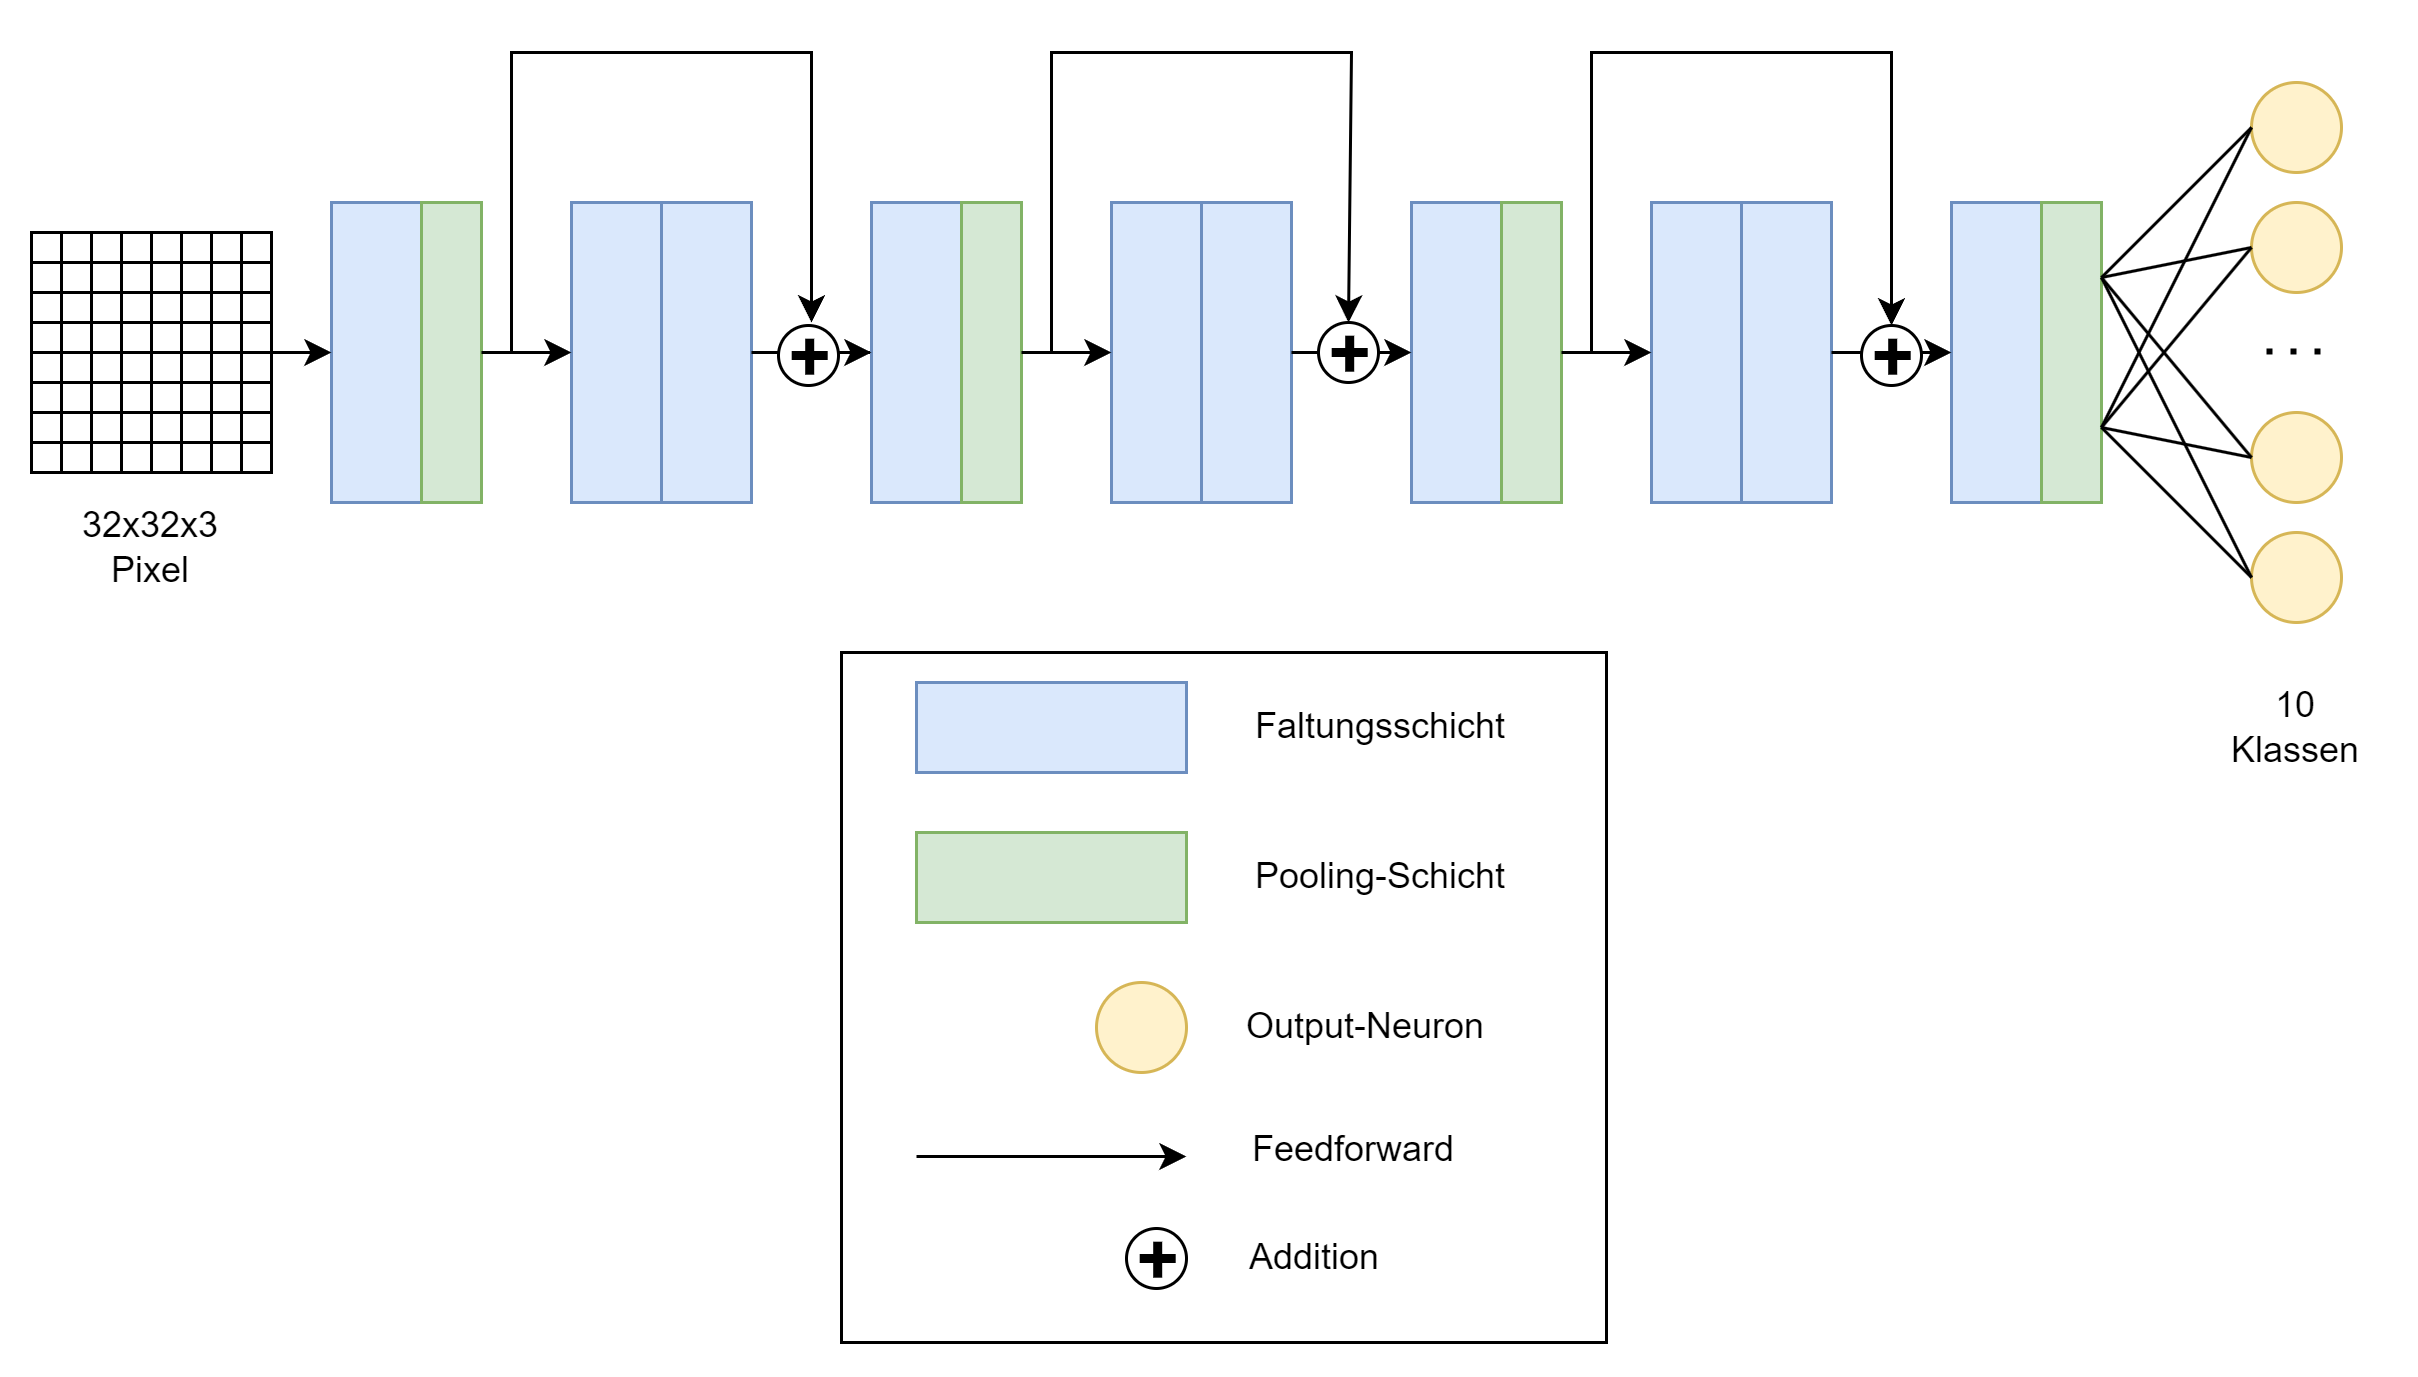
\includegraphics[width=15cm]{figures/cifar_modell.png}
    \caption{Neuronales Netz zur Klassifikation von CIFAR-10}
    \label{fig:cifar_modell}
\end{figure} 

Neben CIFAR-10, wird der CelebA Datenbestand \cite{celeba} genutzt, welcher unter anderem über die Plattform Kaggle zur Verfügung steht.
Dieser enthält 202.599 Bilder, auf welchen jeweils das Gesicht einer Person des öffentlichen Lebens zu sehen ist.
Die Bilder haben jeweils eine Auflösung von $178\times218$ Pixeln mit je 3 Farbkanälen.
Zu jedem Bild gibt es 40 Labels, wobei jedes davon eine Eigenschaft beschreibt. 
Dabei können jeweils die Werte -1 (Eigenschaft nicht vorhanden) und 1 (Eigenschaft vorhanden) angenommen werden.
Ein Beispiel für eine Eigenschaft ist die Größe eines Organs sein (Label \dq \textit{Big\_Nose}\dq).
Manche Eigenschaften können sich außerdem gegenseitig ausschließen.
So gibt es beispielsweise mehrere Labels für Haarfarben (Label \dq \textit{Black\_Hair}\dq\ und Label \dq \textit{Blond\_Hair}\dq).
Der Datenbestand ist bereits unterteilt in \dq \textit{Training}\dq, \dq \textit{Validierung}\dq\ und \dq \textit{Test}\dq.
Die vorgegebene Einteilung wird beibehalten, sodass die Güte des Modells immer auf der Testdatenmenge, welche nicht im Training genutzt werden, gemessen wird.
Tabelle \ref{tab:anzahl_datensaetze} zeigt die Anzahl der Datensätze in den jeweiligen Teildatenbeständen.

\begin{table}[!htb]
\centering
\begin{tabular}{|l|l|l|}
\hline
\rowcolor[HTML]{CBCEFB} 
{\color[HTML]{000000} Datenbestand} & Anzahl Datensätze  & prozentualer Anteil\\ \hline
Training & 162.770  &     $\approx$ 80\%  \\ \hline
Validierung & 19.867 &     $\approx$ 10\%      \\ \hline
Test  & 19.962 &    $\approx$ 10\%    \\ \hline

\end{tabular}
\caption{Anzahl Datensätze}
\label{tab:anzahl_datensaetze}
\end{table}

Der Use Case ist es dabei, alle 40 Label eines Bildes vorherzusagen.
Dabei handelt es sich um ein sogenanntes Multi-Label Klassifizierung, also eine Klassifikation bei der mehrere Klassen (hier Eigenschaften) bestimmt werden können.
Als Metrik zur Messung der Güte eines Modells wird dabei die Genauigkeit genutzt, also das Verhältnis von richtig vorhergesagten Labels zu der gesamten Anzahl an Labels.

Für diesen Use Case werden zwei unterschiedliche Modelle genutzt.
Bei dem ersten Modell handelt es sich um ein ResNet-18 Modell \cite{resnet}.
Dieses hat eine ähnliche Architektur wie das bereits beschriebene Modell für die Klassifizierung der CIFAR-10 Daten.
Jedoch besitzt dieses Modell 18 Faltungsschichten, wodurch die Anzahl der Parameter größer ist.
Das zweite Modell ist das sogenannte Vision Transformer Modell \cite{vit}, kurz ViT. 
Dieses Modell nutzt einige Elemente der Transformer-Architektur, welche ursprünglich aus dem Bereich der Computerlinguistik stammt \cite{transformer}. 
Das Vision Transformer Modell unterteilt das Bild in mehrere, gleich große Teilbilder, welche Patches genannt werden.
Dabei erhalten die Patches eine Position, welche von oben links nach unten rechts inkrementiert wird.
Die Patches werden über sogenannte Embedding-Schichten in einen höherdimensionalen Vektorraum übertragen.
Die entstandenen Vektoren werden Embeddings genannt.
Im Laufe des Trainingsprozesses, werden die Parameter der Embedding-Schichten so angepasst, dass die Ähnlichkeit zweier Embeddings mit der Ähnlichkeit der Eingabebilder korreliert. 
Die Embeddings werden anschließend mit der Position der jeweiligen Patches als Eingabe für einen oder mehrere sequentiell verbundene Kodierer, auch Encoder genannt, genutzt.
Diese bestehen aus jeweils mindestens einem Aufmerksamkeitsmechanismus, auch Attention genannt, und einigen vollständig verbundenen Schichten eines neuronalen Netzes.
Die Aufmerksamkeitsmechanismen erlernen verschiedene Beziehungen der Patches zueinander, welche durch die jeweiligen Positionen in einer räumlichen Verbindung stehen.
Die Ausgabe des letzten Kodierers wird anschließend als Eingabe für vollständig verbundene Schichten genutzt, welche die Klassifikation durchführen.
Neuronen der letzten Schicht repräsentieren jeweils eine Klasse.
\section{Wahl des Frameworks}

Viele der Methoden aus Kapitel \ref{ch:methoden} besitzen ein öffentliches Repository, in denen exemplarisch ein Beispiel umgesetzt und evaluiert wird.
Einige dieser Repositories sind seit Jahren nicht mehr gepflegt, weshalb die Wahl der entsprechenden Bibliotheken entscheidend sein kann.
Bei kryptografischen Methoden empfiehlt sich der Einsatz von bewährten, erforschten und gepflegten Bibliotheken.
Für Homomorphe Verschlüsselung gibt es beispielsweise die SEAL Bibliothek \cite{SEAL}, welche von Microsoft entwickelt wird, oder auch die HElib \cite{helib}.
Diverse Secure Multi-Party Computation Methoden, wie Yao's Garbled Circuits, werden in einer Bibliothek namens MP-SPDZ \cite{mp-spdz} implementiert.
Allerdings sind Bibliotheken für funktionale Verschlüsselung weniger gepflegt. So hat die Bibliothek CiFEr \cite{cifer} seit mehr als zwei Jahren keine Aktualisierung erhalten.

Um Differential Privacy zu nutzen, ist nicht zwingend eine spezialisierte Bibliothek notwendig. 
Die populäre Python Bibliothek NumPy \cite{numpy}, die in vielen Machine Learning Projekten eingesetzt wird, bietet bereits Funktionalität, um beispielsweise Werte mittels einer Laplace-Verteilung oder Gauß-Verteilung zu verrauschen.
Lediglich die Berechnung des Privacy Budgets fehlt in NumPy.

Die größten Frameworks für die Entwicklung von neuronalen Netzen sind PyTorch \cite{pytorch}, TensorFlow \cite{tensorflow} und JAX \cite{jax}. 
Tabelle \ref{tab:framworks} zeigt die Anzahl der Modelle, die jeweils mit dem entsprechenden Framework trainiert wurden und auf Hugging Face, einer Plattform zum Teilen von neuronalen Netzen, hochgeladen wurden \cite{HuggingFace}.
Das Framework PyTorch wurde dabei für fast 7 Mal so viele Modelle genutzt, wie die anderen beiden Frameworks zusammen.
\begin{table}[!htb]
\centering
\begin{tabular}{|l|l|}
\hline
\rowcolor[HTML]{CBCEFB} 
{\color[HTML]{000000} Framework} & Anzahl Modelle auf Hugging Face     \\ \hline
PyTorch & 122.061          \\ \hline
TensorFlow & 9.326             \\ \hline
JAX  & 8.560          \\ \hline

\end{tabular}
\caption{Anzahl Modelle je Framework auf Hugging Face \cite{HuggingFace}}
\label{tab:framworks}
\end{table}

PyTorch und TensorFlow besitzen beide ein offizielles Modul, welches den Einsatz von Differential Privacy während des Trainings eines neuronalen Netzes ermöglicht. 
Diese heißen Opacus \cite{opacus} und TensorFlow Privacy \cite{Tensorflowprivacy}.
Für das Framework JAX gibt es keine offizielle Erweiterung für Differential Privacy, lediglich ein paar Open-Source-Bibliotheken wie JAX-Privacy \cite{jaxprivacy}.
Für die nachfolgenden Experimente wird das Framework PyTorch mit der Erweiterung Opacus genutzt.
\section{Technische Implementierung von DPSGD}\label{sec:opacu_implementierung}
Opacus ist eine Bibliothek, welches das Framework PyTorch erweitert, indem das Training eines neuronalen Netzes mittels DPSGD ermöglicht wird \cite{opacus}.
Der Großteil des PyTorch Codes bleibt dabei unverändert, wird jedoch um einige Wrapper-Klassen der Opacus Bibliothek erweitert.

\begin{lstlisting}[language=Python,caption={Training einer Epoche in PyTorch},captionpos=b,showstringspaces=false,label={lst:torch_default}]
import torch

model:torch.nn.Module = <...> 
criterion:torch.nn.Module._Loss = torch.nn.CrossEntropyLoss()
optimizer:torch.optim.Optimizer = torch.optim.Adam(model.parameters(), 
                                                   lr=0.01)
train_dataloader:torch.utils.data.DataLoader = <...> 

for epoch in range(10):
    for inputs, labels in train_dataloader:
        optimizer.zero_grad()
        model_outputs = model(inputs)
        loss = criterion(model_outputs, labels)
        loss.backward()
        optimizer.step()
\end{lstlisting}

Listing \ref{lst:torch_default} zeigt die wichtigsten Komponenten beim Training eines neuronalen Netzes mit PyTorch.
Die Zeilen 3 bis 7 definieren die Objekte, die für das Training genutzt werden. 
Das Modell, welches trainiert werden soll, ist dabei vom Datentyp \textbf{torch.nn.Module} und wird in Zeile 3 als Platzhalter definiert.
Zeile 4 definiert die Verlustfunktion, welche in diesem Beispiel \textbf{torch.nn.CrossEntropyLoss} ist.
Als \textbf{Optimizer} wird \textbf{torch.optim.Adam} in Zeile 5 und 6 deklariert.
Bei einem \textbf{Dataloader} handelt es sich um ein Objekt, welches Batches von Datensätzen und die zugehörigen Labels über einen Iterator ausgibt.
Die Zeilen 10 bis 15 trainieren eine Epoche. 
Dabei wird jeder Batch, welche von dem \textbf{Dataloader} in Zeile 10 stammen, durch das Modell inferiert (Zeile 12). 
Mittels der Verlustfunktion werden die Gradienten der einzelnen Gewichte bestimmt (Zeile 13 und 14).
Der \textbf{Optimizer} passt anschließend die Gewichte in die entgegengesetzte Richtung der Gradienten, skaliert mit der Lernrate, an (Zeile 15).
Das Einbetten der Trainingslogik in eine For-Schleife ermöglicht das Training mehrerer Epochen hintereinander.

Opacus bietet Wrapper-Klassen, welche die Nutzung von DPSGD ermöglicht. 
Listing \ref{lst:opacus_pe1} zeigt, wie diese genutzt werden.
Zuerst wird ein Objekt des Typs \textbf{PrivacyEngine} in Zeile 3 deklariert.
Der Parameter \dq \textit{rdp}\dq \ als \dq \textit{accountant}\dq \ sorgt dafür, dass die Moments Berechnung aus Kapitel \ref{sec:dp_training} verwendet wird.
Die \textit{make\_private()}-Methode der \textbf{PrivacyEngine} akzeptiert das \textbf{Modell}, den \textbf{Optimizer} und den \textbf{Dataloader} und gibt diese jeweils in einer Wrapper-Klasse zurück.
Das Modell ist anschließend vom Datentyp \textbf{GradSampleModule\mbox} der Opacus Bibliothek. 
Normale PyTorch Modelle, vom Typ \textbf{torch.nn.Module\mbox}, berechnen aggregiert die Gradienten pro Batch, wohingegen die Wrapper-Klasse von Opacus\mbox, \textbf{GradSampleModule\mbox}, für jeden Datensatz eines Batches die Gradienten berechnet.
Grund dafür ist, dass die einzelnen Gradienten für das Clipping und das Verrauschen benötigt werden \cite{P-28}.
Das Clipping und Verrauschen übernimmt jedoch die Wrapper-Klasse des Optimizers. 
Diese ist vom Datentyp \textbf{DPOptimizer} der Opacus Bibliothek.
Der PyTorch \textbf{Dataloader\mbox} wird zu einem Opacus \textbf{DPDataloader} transformiert, welcher anschließend Batches mittels des Poisson-Samplings zusammenstellt.
Die \textit{make\_private()}-Methode benötigt noch zwei weitere Parameter: \textit{max\_grad\_norm} und \textit{noise\_multiplier}. 
Bei dem Wert von \textit{max\_grad\_norm} handelt es sich um die maximale Größe eines Gradienten, welche durch das Clipping beschränkt wird.
Der \textit{noise\_multiplier} definiert dabei die Stärke des Rauschens.
Diese wird mit der \textit{max\_grad\_norm} multipliziert und anschließend als Standardabweichung $\sigma$ des Gauß-Mechanismus, welcher für das Verrauschen der Gradienten zuständig ist, genutzt.

\begin{lstlisting}[language=Python,caption={Opacus Wrapper für DPSGD},captionpos=b,showstringspaces=false,label={lst:opacus_pe1}]
import opacus

privacy_engine = opacus.PrivacyEngine(accountant="rdp")
model, optimizer, data_loader = privacy_engine.make_private(
    module=model,
    optimizer=optimizer,
    data_loader=data_loader,
    noise_multiplier=1.0,
    max_grad_norm=1.0
)
#Hinterher normales Training des Modells
\end{lstlisting}

Nachdem die \textit{make\_private()}-Methode aufgerufen wurde und die entsprechenden Objekte von Opacus in Wrapper-Klassen umgewandelt wurden, wird das Modell mit gewöhnlichen PyTorch Code (Listing \ref{lst:torch_default}) trainiert. 
Um den $\epsilon$-Wert des Privacy Budgets zu begrenzen, kann nach jedem Training eines Batches oder einer Epoche der aktuelle $\epsilon$-Wert abgefragt werden und beim Überschreiten eines Grenzwerts das Training vorzeitig beendet werden.
Listing \ref{lst:calc_epsilon} zeigt den entsprechenden Methodenaufruf.
Dabei wird der $\delta$-Wert des Privacy Budgets als Parameter mitgegeben. 
Dieser wird im Voraus definiert und sollte kleiner als die Inverse der Anzahl an Datensätzen des Trainingsdatenbestands sein.

\begin{lstlisting}[language=Python,caption={Berechnung von Epsilon},captionpos=b,showstringspaces=false,label={lst:calc_epsilon}]
privacy_engine.accountant.get_epsilon(delta=1e-5)
\end{lstlisting}

Ein Nachteil der Nutzung der \textit{make\_private()}-Methode besteht darin, dass ein Wert für das Rauschen im Voraus festgelegt werden muss.
Bei einer zufälligen Wahl dieses Werts, ist unklar, wie viele Epochen trainiert werden können, bevor ein gewisses Privacy Budget überschritten wird. 
Um dieses Problem zu umgehen, kann als Alternative die Methode \textit{make\_private\_with\_epsilon()\mbox} genutzt werden.
Diese ist in Listing \ref{lst:opacus_pe2} zu sehen.
Anstatt dass hier eine Stärke des Rauschens übergeben wird, werden die gewünschte Anzahl an Epochen sowie das gewünschte Privacy Budget angegeben.
Anschließend berechnet Opacus die Stärke des Rauschens, sodass in etwa nach der festgelegten Anzahl an Epochen das Privacy Budget erreicht ist.
Jedoch kann der Wert des Privacy Budgets leicht abweichen. 
Dies liegt daran, dass durch das Poisson-Sampling die Anzahl an Datensätzen je Batch abweichen kann. 
Dadurch werden unterschiedlich viele Gradienten in jeder Epoche verrauscht.
Die Abweichung ist deshalb bei einer kleinen Anzahl an Epochen am größten.
Im Durchschnitt sollte die Größe der Batches jedoch der konfigurierten Batch-Größe entsprechen, sodass sich diese Abweichung über mehrere Epochen hinweg ausgleicht.


\begin{lstlisting}[language=Python,caption={Opacus Wrapper mit definiertem Epsilon},captionpos=b,showstringspaces=false,label={lst:opacus_pe2}]
import opacus

privacy_engine = opacus.PrivacyEngine(accountant="rdp")
model, optimizer, data_loader = privacy_engine.make_private_with_epsilon(
    module=model,
    optimizer=optimizer,
    data_loader=data_loader,
    epochs=10,
    target_epsilon=10,
    target_delta=1e-5,
    max_grad_norm=1.0
)
#Hinterher normales Training des Modells
\end{lstlisting}



\subsubsection*{Einschränkungen der Modellarchitektur}

Nicht jede Schicht eines Modells wird von DPSGD unterstützt und kann deshalb genutzt werden. 
Opacus bietet eine Klasse \textbf{ModuleValidator\mbox} an, welche überprüft, ob ein Modell kompatibel ist und bei Bedarf inkompatible Schichten austauscht.
Listing \ref{lst:modulevalidator} zeigt, wie diese Klasse genutzt werden kann.
Die \textit{validate()}-Methode aus Zeile 1 gibt dabei lediglich eine Liste mit inkompatiblen Schichten, sowie jeweils einer kurzen Erklärung dazu, zurück.
Um die inkompatiblen Schichten mit kompatiblen, alternativen Schichten ausgetauscht werden, kann die \textit{fix()}-Methode aufgerufen werden. 
\begin{lstlisting}[language=Python,caption={Opacus ModuleValidator} ,captionpos=b,showstringspaces=false,label={lst:modulevalidator}]
incompatible_layers = opacus.validators.ModuleValidator.validate(model)
model = opacus.validators.ModuleValidator.fix(model)
\end{lstlisting}

Ein Beispiel für eine nicht kompatible Schicht ist die sogenannte \textbf{BatchNorm}-Schicht.
Diese Schicht berechnet Mittelwerte und Standardabweichung über mehrere Datensätze eines Batches und nutzt diese anschließend für die Normalisierung der Datensätze.
Folglich wird ein Datensatz durch andere Datensätze in dem gleichen Batch beeinflusst, was jedoch nicht gewünscht ist. 
Dies liegt daran, dass laut DPSGD (Kapitel \ref{sec:dp_training}) ein Datensatz ($\epsilon$,$\delta$)-Differential Privacy in Bezug auf einen Batch erfüllen soll \cite{P-28}.
Alternative Schichten sind die \textbf{LayerNorm}-Schicht, die \textbf{InstanceNorm}-Schicht oder die \textbf{GroupNorm}-Schicht.
All diese Schichten dienen ebenfalls der Normalisierung, jedoch nicht anhand anderer Datensätze eines Batches \cite{opacus_blog_part3}.

\subsubsection*{Laufzeit und Speicherverbrauch}
Wie bereits erwähnt, berechnen normale PyTorch Modelle die Gradienten der Gewichte aggregiert über einen Batch.
Der Grund dafür ist die Performance, denn die Berechnung von Gradienten einzelner Datensätze, ist beim Training ohne Differential Privacy nicht nötig. 
DPSGD benötigt jedoch genau diese Gradienten einzelner Datensätze, um diese per Clipping und Verrauschen zu verändern \cite{P-28}, weshalb diese in Opacus berechnet werden \cite{opacus}.
Jedoch sorgt dies für eine längere Laufzeit, sowie einen erhöhten Speicherverbrauch.

Der Faktor, um welchen sich die Laufzeit erhöht, hängt dabei primär von den Arten der Schichten eines neuronalen Netzes ab. 
Faltungsschichten, Normalisierungsschichten und sogenannte Multi-Head-Attention-Schichten sorgen für eine Erhöhung der Laufzeit um den Faktor 1,2 bis 2,9.
Bei vollständig verbundenen Schichten und den sogenannten Embedding-Schichten\mbox, skaliert der Faktor der Laufzeit mit der Batch-Größe \cite{opacus}.
Der Speicherverbrauch skaliert ebenfalls mit der Batch-Größe.
Dies liegt daran, dass für jedes Gewicht nicht nur ein Gradient im Speicher gehalten wird, sondern jeweils ein Gradient für jeden Datensatz eines Batches \cite{opacus}.

Das Poisson-Sampling von DPSGD sorgt dafür, dass die tatsächliche Batch-Größe von der festgelegten Batch-Größe abweichen kann. 
Dies kann jedoch zu einem Problem werden, wenn die festgelegte Batch-Größe so ausgewählt wurde, dass der zur Verfügung stehende Speicher der GPU nahezu vollständig ausgenutzt wird.
Weicht die Batch-Größe nach oben ab, hat also mehr Datensätze als festgelegt, kann es sein, dass der Speicher nicht ausreicht und eine sogenannte \textbf{OutOfMemoryException} geworfen wird.
Dies sorgt für einen Abbruch des Trainings, woraufhin der Speicher geleert werden müsste und das Training neu gestartet werden müsste.
Um dies zu verhindert, bietet Opacus eine Lösung in Form der Klasse \textbf{BatchMemoryManager} an.
Diese Klasse wrappt den Dataloader nochmals in eine Wrapper-Klasse, bei welcher ein Parameter \dq \textit{max\_physical\_batch\_size}\dq\ mitgegeben wird. 
Der neue, zurückgegebene Dataloader beschränkt die tatsächliche Batch-Größe auf die als Maximum festgelegte Batch-Größe, sodass ein Überlaufen des Speichers verhindert wird.
Listing \ref{lst:memory_manager} zeigt, wie der BatchMemoryManager in den Trainingsprozess integriert wird.
Außerdem kann dieser auch genutzt werden, um mit virtuellen Batches zu trainieren. 
Dabei kann die Batch-Größe des Dataloaders höher konfiguriert werden, als die maximale Batch-Größe des BatchMemoryManagers. 
Dies sorgt dafür, dass die einzelnen Gradienten jeden Datensatzes anhand der kleineren Batches des BatchMemoryManagers berechnet werden.
Jedoch erfolgt die Aggregierung der Gradienten und das Anpassen der Gewichte erst, wenn die konfigurierte Batch-Größe des Dataloaders erreicht wurde.

\begin{lstlisting}[language=Python,caption={Opacus BatchMemoryManager},captionpos=b,showstringspaces=false,label={lst:memory_manager}]
with BatchMemoryManager( 
    data_loader=train_dataloader,
    max_physical_batch_size=64,
    optimizer=optimizer) 
as memory_safe_data_loader:
        for model_inputs,labels in mmemory_safe_data_loader:
            # Training ...
\end{lstlisting}

Tabelle \ref{tab:memory} zeigt, wie hoch der Speicherverbrauch bei den bereits beschriebenen Use Cases ist. 
Dabei wird der Speicher der Grafikkarte, auch VRAM genannt, betrachtet, da dieser oftmals ein limitierender Faktor ist.
Für das CIFAR-10 Modell, welches eine ResNet-Architektur nutzt, steigt der Speicherverbrauch bei der Nutzung von DPSGD mit Opacus um den Faktor 1,8 bis 5,0.
Für beide Modelle, welche Merkmale aus Gesichtern erkennen, wurde jeweils nur eine Batch-Größe betrachtet.
Dabei ist die Batch-Größe eine Zweierpotenz, die so gewählt ist, dass der entsprechende Batch mit DPSGD und Opacus noch in den Speicher passt. 
Der maximale Speicher der genutzten Hardware liegt bei 24 GB VRAM (siehe Anhang \ref{ch:hard_software}).
Der Speicherverbrauch des ResNet-18-Modells steigt um den Faktor 2,8 bei einer Batch-Größe von 64.
Für das Vision Transformer Modell kann jedoch nur eine Batch-Größe von 16 ausgewählt werden, da hier mit 20,8 GB Speicherauslastung fast das Limit der Hardware erreicht ist.
Die relativ geringe Batch-Größe sorgt lediglich für eine Differenz von 1,6 Mal so viel Speicherauslastung, wie ohne DPSGD.
\begin{table}[!htb]
\centering
\begin{tabular}{|l|l|l|l|l|}
\hline
\rowcolor[HTML]{CBCEFB} 
Modell                   & Batch-Größe & \begin{tabular}[c]{@{}l@{}}Speicherverbrauch\\ ohne DPSGD\end{tabular} & \begin{tabular}[c]{@{}l@{}}Speicherverbrauch\\ mit DPSGD\end{tabular} & \begin{tabular}[c]{@{}l@{}}Faktor \\ Differenz\end{tabular} \\ \hline
CIFAR-10 Modell          & 64          & 2,8 GB VRAM                                                         & 5,1 GB VRAM                                                         & 1,8                                                         \\ \hline
CIFAR-10 Modell          & 128         & 2,9 GB VRAM                                                          & 10,2 GB VRAM                                                        & 3,5                                                         \\ \hline
CIFAR-10 Modell          & 256         & 3,3 GB VRAM                                                          & 16,4 GB VRAM                                                        & 5,0                                                           \\ \hline
CelebA ResNet-18          & 64          & 4,6 GB VRAM                                                          & 12,8 GB VRAM                                                        & 2,8                                                         \\ \hline
CelebA ViT & 16          & 12,8 GB VRAM                                                         & 20,8 GB VRAM                                                        & 1,6                                                         \\ \hline
\end{tabular}
\caption{Speicherverbrauch mit und ohne Differential Privacy}
\label{tab:memory}
\end{table}

Tabelle \ref{tab:memory} zeigt, wie die Trainingsdauer einer Epoche für die Modelle variieren kann.
Dabei wurden die gleichen Batch-Größen gewählt, wie bei der Messung des Speicherverbrauchs.
Die Trainingsdauer des CIFAR-10 Modells erhöht sich um einen Faktor von 1,3 bis 3,1.
Da eine Epoche jedoch nur wenige Sekunden benötigt, fällt die absolute Differenz relativ gering aus.
Die Modelle der Merkmalserkennung sind demgegenüber komplexer und benötigen ohne DPSGD bereits mehrere Minuten für das Training einer Epoche. 
Jedoch erhöht sich der Faktor hier auf 4,5 oder 10,0. 
Dies liegt zum einen an den Arten der Schichten und zum anderen an einem Softwarefehler des Frameworks.
Das ResNet-18-Modell nutzt einige Normalisierungsschichten, das Vision Transformer Modell nutzt einige Multi-Head-Attention Schichten für die Implementierung eines Aufmerksamkeitsmechanismus.
Die zusätzliche Laufzeit dieser Schichten, skaliert bei Opacus mit der Batch-Größe, wodurch hier ein höherer Multiplikationsfaktor entstehen kann.
Zusätzlich gibt es einen Softwarefehler des Dataloaders in Kombination mit Opacus, welcher dazu führt, dass das Laden von Daten nur in einem Thread ausgeführt werden kann und nicht zeitgleich in mehreren.
Der Fehler wird im folgenden genauer beleuchtet.
Der gleiche Fehler existiert auch bei den CIFAR-10 Modellen, fällt da jedoch weniger ins Gewicht, da das Laden der Bilder aufgrund der geringeren Auflösung weniger Zeit benötigt.
\begin{table}[!htb]
\centering
\begin{tabular}{|l|l|l|l|l|}
\hline
\rowcolor[HTML]{CBCEFB} 
Modell                    & Batch-Größe & \begin{tabular}[c]{@{}l@{}}Dauer Epoche\\ ohne DPSGD\end{tabular} & \begin{tabular}[c]{@{}l@{}}Dauer Epoche\\ mit DPSGD\end{tabular} & \begin{tabular}[c]{@{}l@{}}Faktor \\ Differenz\end{tabular} \\ \hline
CIFAR-10 Modell           & 64          & 7 Sekunden                                                     & 22 Sekunden                                                   & 3,1              \\ \hline
CIFAR-10 Modell           & 128         & 7 Sekunden                                                     & 18 Sekunden                                                   & 2,6              \\ \hline
CIFAR-10 Modell           & 256         & 14 Sekunden                                                    & 18 Sekunden                                                   & 1,3              \\ \hline
CelebA ResNet-18           & 64          & 3 Minuten                                                      & 30 Minuten                                                    & 10,0               \\ \hline
CelebA ViT & 16          & 11 Minuten                                                     & 50 Minuten                                                    & 4,5              \\ \hline
\end{tabular}
\caption{Dauer des Trainings einer Epoche mit und ohne Differential Privacy}
\label{tab:dauer_epoch}
\end{table}

\subsubsection*{Softwarefehler}

Da Opacus eine optionale Erweiterung von PyTorch ist, ist die Bibliothek weniger genutzt.
Dies ist über die Statistiken von GitHub erkennbar. 
Während es auf GitHub fast 304.000 Repositories gibt, die PyTorch benutzen\footnote{https://github.com/pytorch/pytorch}, sind es bei Opacus lediglich knapp 600\footnote{https://github.com/pytorch/opacus}.
Laut diesen Zahlen, nutzen nur \ca 0,2 \% der Projekte mit PyTorch zusätzlich noch Opacus.
Dies kann ein Grund sein, warum deutlich weniger Ressourcen in die Entwicklung von Opacus fließen.
Bei PyTorch haben fast 3000 Personen über GitHub etwas zur Entwicklung des Frameworks beigetragen, wohingegen bei Opacus lediglich 55 Personen beteiligt waren.
Dies könnte ein Grund sein, warum Opacus einige Softwarefehler hat, oder warum einige Features nicht vollumfänglich funktionieren.

Ein Softwarefehler, der die Trainingsdauer der Epoche erhöht, entsteht bei der Parallelisierung des Dataloaders.
Der Dataloader kann über einen Parameter \dq\textit{num\_workers}\dq\ eine vorgegebene Anzahl an Threads starten. 
Jeder dieser Threads lädt dabei einen Batch an Datensätzen in den Speicher, sodass nach dem Training eines Batches bereits der nächste Batch zur Verfügung steht.
Durch die Wrapper-Klasse in Opacus, welche das Poisson-Sampling implementiert, ist diese Parallelisierung nicht mehr möglich.
Dies sorgt dafür, dass wenn die GPU einen Batch zum Training genutzt hat, es sein kann, dass der nächste Batch noch nicht geladen ist und somit die GPU auf diesen warten muss.
Je komplexer die Daten und die Prozesse des Ladens sind, desto länger dauert das Laden eines Batches.
Bei dem CelebA Datenbestand muss jedes Bild, welches jeweils eine Dimension von $178\times218\times3$ hat, von der Festplatte der Hardware geladen werden.
Dies ist der Grund, warum das CelebA ResNet-18-Modell mit DPSGD die 10-fache Trainingsdauer einer Epoche erreicht, als im Vergleich zum Training ohne DPSGD.

Ein Beispiel für ein Feature, welches nicht vollumfänglich funktioniert, ist die Nutzung eines adaptiven Werts für das Clipping.
Die Technik mit dem Namen AdaClip sorgt dafür, dass die Clipping-Norm variabel ist und sich den Gradienten anpasst \cite{adaclip}.
Dadurch könnte der Wert möglichst gering sein, was auch das hinzugefügte Rauschen verkleinern würde.
Die Klasse, welche die entsprechende Logik enthält, existiert in Opacus unter dem Namen \textbf{AdaClipDPOptimizer}.
Jedoch gibt es zwei Probleme, welche die Nutzung der Klasse erschweren oder nicht möglich machen.
Das erste Problem ist, dass die Übergabe der Parameter nicht korrekt funktioniert. 
Die \textit{make\_private()}-Methode kann über den Parameter \dq\textit{clipping}\dq\ mit dem Wert \dq\textit{adaptive}\dq\ so aufgerufen werden, dass der AdaClipDPOptimizer genutzt werden würde.
Jedoch braucht diese Klasse zusätzliche Parameter, welche nicht über die \textit{make\_private()}-Methode weitergegeben werden können.
Um dieses Problem zu umgehen, müssen die Wrapper-Klassen manuell konfiguriert werden.
Das zweite Problem liegt in der Klasse selber.
PyTorch hat einige Kontrollen integriert, welche sicherstellen sollen, dass das Training in einem vorgegebenen Rahmen ausgeführt wird. 
Eine dieser Kontrollen ist es, dass die Gradienten vor dem Training eines Batches zurückgesetzt werden, damit Gradienten nicht mehrfach genutzt werden.
Bei Nutzung der Klasse AdaClipDPOptimizer kommt es jedoch zu einem Fehler dieser Kontrolle.

Obwohl die Behebung diverser Fehler und das Hinzufügen fehlender Funktionalität große Relevanz hat, ist dies im Rahmen der Arbeit nicht möglich.
Deshalb werden mögliche Fehler umgangen.
Die nicht mögliche Parallelisierung des Dataloaders schränkt die Funktionalität nicht ein, sondern erhöht nur die Laufzeit. 
Im Gegensatz dazu, ist die Nutzung der adaptiven Clipping-Norm nicht ohne entsprechenden Aufwand möglich, weshalb im folgenden lediglich konstante, festgelegte Werte für das Clipping betrachtet werden.


\section{Hyperparameter von DPSGD}\label{sec:hyperparams}

Die Güte eines Modells wird durch die Wahl der Hyperparameter beeinflusst. 
Dies gilt sowohl beim normalen Training, als auch beim Training mit DPSGD.
Im Folgenden wird getestet, welche Parameter die Güte eines neuronalen Netzes bei der Nutzung von DPSGD beeinflussen.
Dazu werden die drei Modelle, welche in Kapitel \ref{sec:use_case} beschrieben wurden, mit verschiedenen Hyperparametern trainiert und evaluiert.
Dabei werden DPSGD spezifische Parameter, wie der $\epsilon$-Wert und die Clipping-Norm, und auch allgemeine Parameter, wie die Batch-Größe und die Anzahl der Epochen, betrachtet.
Die Lernrate wird dabei nicht konstant festgelegt, sondern über den \textbf{Adam}-Optimizer in PyTorch adaptiv konfiguriert.
Der Adam-Optimizer passt die Lernrate anhand des Momentums und der Varianz der Gradienten an \cite{adam}.

Bevor das eigentliche Modell trainiert wird, gibt es die Möglichkeit, die Datenmenge per Datenaugmentierung, auch Data Augmentation genannt, künstlich zu erweitern.
Bei Bildern können die Werte einzelner Pixeln beeinflusst werden, indem der Farbraum der Bilder angepasst wird, oder Kontraste erhöht werden.
Zusätzlich können Bilder über Rotation und Spieglung transformiert werden.
Dabei können die Werte der Anpassung, \zB die Verstärkung des Kontrasts, konfiguriert werden und an eine Wahrscheinlichkeit geknüpft werden.
PyTorch bietet über AutoAugment eine Möglichkeit an, eine Kombination verschiedener Anpassungen zu nutzen \cite{autoaugment}.
Die Nutzung von AutoAugment, sowie dessen Einfluss auf die Güte der Modelle, wird folglich mitberücksichtigt.

Da das CIFAR-10 Modell die geringste Anzahl an lernbaren Parameter besitzt, wird die Anpassung verschiedener Parameter an diesem Modell zuerst evaluiert.
Anschließend werden die Erkenntnisse auf das ResNet-18 Modell und das Vision Transformer Modell für den CelebA Datenbestand angewendet.
Im Folgenden werden einige Auszüge aus den gesamten Ergebnissen zur Veranschaulichung herangezogen. 
Die vollständigen Tabellen aller Messwerte befinden sich in Anhang \ref{ch:ergebnisse_detail}.

\subsection{Hyperparameter CIFAR-10 Modell}

Für das CIFAR-10 Modell, welches kein DPSGD nutzt, werden folgende Hyperparameter betrachtet: Anzahl der Epochen, Batch-Größe und die Nutzung von AutoAugment.
Dazu wurde das Modell mit einer Epochenanzahl zwischen 10 und 20 trainiert, jeweils mit einer Batch-Größe von 64, 128 oder 256. 
Dieser Vorgang wurde mit AutoAugment aktiviert und deaktiviert ausgeführt.
Die höchste Genauigkeit wird erreicht, wenn das Modell mit Datenugmentierung und einer Batch-Größe von 64 über 15 Epochen hinweg trainiert wird.
Die erreichte Genauigkeit, welche anhand der Test-Daten gemessen wurde, liegt bei 84,6 \%.

Eine Batch-Größe von 64 und 128 resultieren in einer ähnlichen Güte des Modells. 
Jedoch sorgt eine Batch-Größe von 256 für eine geringere Genauigkeit des Modells. 
Dies liegt daran, dass einzelne Datensätze in der Aggregation der Gradienten untergehen können, wodurch einzelne Features der Daten weniger gut gelernt werden. 
Abbildung \ref{fig:cifar-1} zeigt die Güte der Modelle, welche mit den unterschiedlichen Batch-Größen trainiert wurden.
Jede Linie steht dabei für eine unterschiedliche Anzahl an trainierten Epochen.
\begin{figure}[!htb]
    \centering
    \fbox{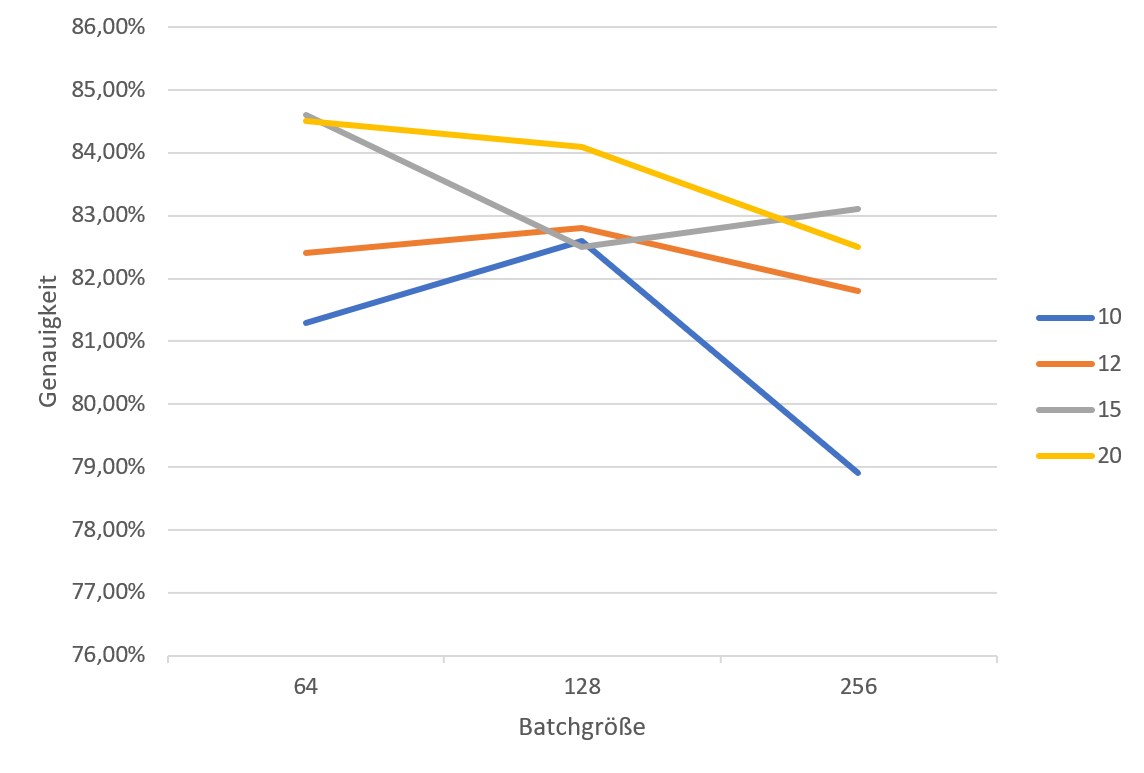
\includegraphics[width=14cm]{figures/results_cifar/cifar_batch_base.png}}
    \caption{Auswirkung Batch-Größe auf CIFAR-10 Modell ohne DPSGD und mit \\Datenaugmentierung}
    \label{fig:cifar-1}
\end{figure} 

Zusätzlich zeigt Abbildung \ref{fig:cifar-1}, dass eine höhere Anzahl an Epochen mit einer höheren Genauigkeit korreliert.
Dies liegt an der Nutzung von Datenaugmentierung. 
Wird diese nicht genutzt, liegt die optimale Anzahl an Epochen zwischen 12 und 15. 
Werden mehr Epochen trainiert, sinkt die Genauigkeit wieder, was auf ein Overfitting des Modells zurückzuführen ist.
Generell sinkt die Genauigkeit der Modelle, wenn AutoAugment nicht genutzt wird. 
Durch die Datenaugmentierung wird der Datensatz künstlich erweitert, was dafür sorgt, dass die Trainingsdatenmenge vergrößert wird.

Für das CIFAR-10 Modell ohne DPSGD resultieren folgendende Hyperparameter in einer optimalen Güte des Modells:
\begin{compactitem}
    \item \textbf{Batch-Größe:} Batch-Größe kann variablen gewählt werden, sollte jedoch nicht zu groß sein. Ein Wert von 64 oder 128 ist wirksam.
    \item \textbf{Anzahl Epochen:} Die optimale Anzahl an Epochen ist um 15 herum. Wird Datenaugmentierung genutzt, kann die Anzahl höher sein, wenn nicht, dann sollte die Anzahl geringer sein.
    \item \textbf{Datenaugmentierung:} Datenaugmentierung verbessert die Güte des Modells und ermöglicht das Training mehrerer Epochen, wobei Overfitting vermieden wird. Datenaugmentierung sollte deshalb genutzt werden.
\end{compactitem}


Wird das CIFAR-10 Modell mit DPSGD trainiert, müssen zusätzlich noch der $\epsilon$-Wert des Privacy Budgets und die Clipping-Norm betrachtet werden. 
Der $\delta$-Wert des Privacy Budgets wird konstant auf $10^{-5}$ festgelegt.
Um die Hyperparameter zu evaluieren, gibt es drei unterschiedliche Versuche.
Alle drei Versuche trainieren eine Vielzahl an Modellen mit DPSGD.
Dabei werden $\epsilon$-Werte von 1 bis 50, Epochenanzahlen von 1 bis 30 und Batch-Größen von 64 bis 256 genutzt.
Lediglich bei der Clipping-Norm und bei der Nutzung von Datenaugmentierung unterscheiden sich die drei Versuche.
Um den festgelegten $\epsilon$-Wert nach einer festgelegten Anzahl an Epochen zu erreichen, wurde die \textit{\mbox{make\_private\_with\_epsilon()}}-Methode genutzt.

Der erste Versuch nutzt Datenaugmentierung und hat einen nicht optimierten Wert der Clipping-Norm.
Dieser ist auf 1,0 festgelegt.
Dieser Versuch zeigt, dass die Genauigkeit der Modelle, mit der Größe des $\epsilon$-Werts zunimmt.
Bei einem $\epsilon$-Wert von 1 wird maximal eine Genauigkeit von 36,9 \% erreicht, wohingegen bei einem $\epsilon$-Wert von 50 eine Genauigkeit von 59,1 \% erreicht wird.
Ebenfalls steigt die Genauigkeit der Modelle mit der Anzahl an trainierten Epochen. 
Dies liegt daran nicht nur daran, dass Datenaugmentierung genutzt wird, sondern dass auch das Rauschen Overfitting verhindert.
Sogar 30 Epochen können trainiert werden, ohne dass die Genauigkeit stagniert.
Anders als bei dem Modell ohne DPSGD, hat die Batch-Größe eine deutliche Auswirkung auf die Genauigkeit der Modelle.
Eine höhere Batch-Größe sorgt für eine verbesserte Genauigkeit der Modelle.
Das Rauschen, welches den einzelnen Gradienten hinzugefügt wird, gleicht sich bei einer höheren Batch-Größe aus und nähert sich dem Erwartungswert an. 
Da der Erwartungswert den echten Gradienten entspricht, bedeutet dies, dass eine höhere Batch-Größe dafür sorgt, dass die verrauschten Gradienten der Gewichte, näher an den tatsächlichen Gradienten der Gewichte liegen.
Abbildung \ref{fig:cifar-2} zeigt diesen Zusammenhang grafisch.
Jede Linie entspricht einem Modell, welches über 15 Epochen, mit unterschiedlichem $\epsilon$-Wert, trainiert wird.
\begin{figure}[!htb]
    \centering
    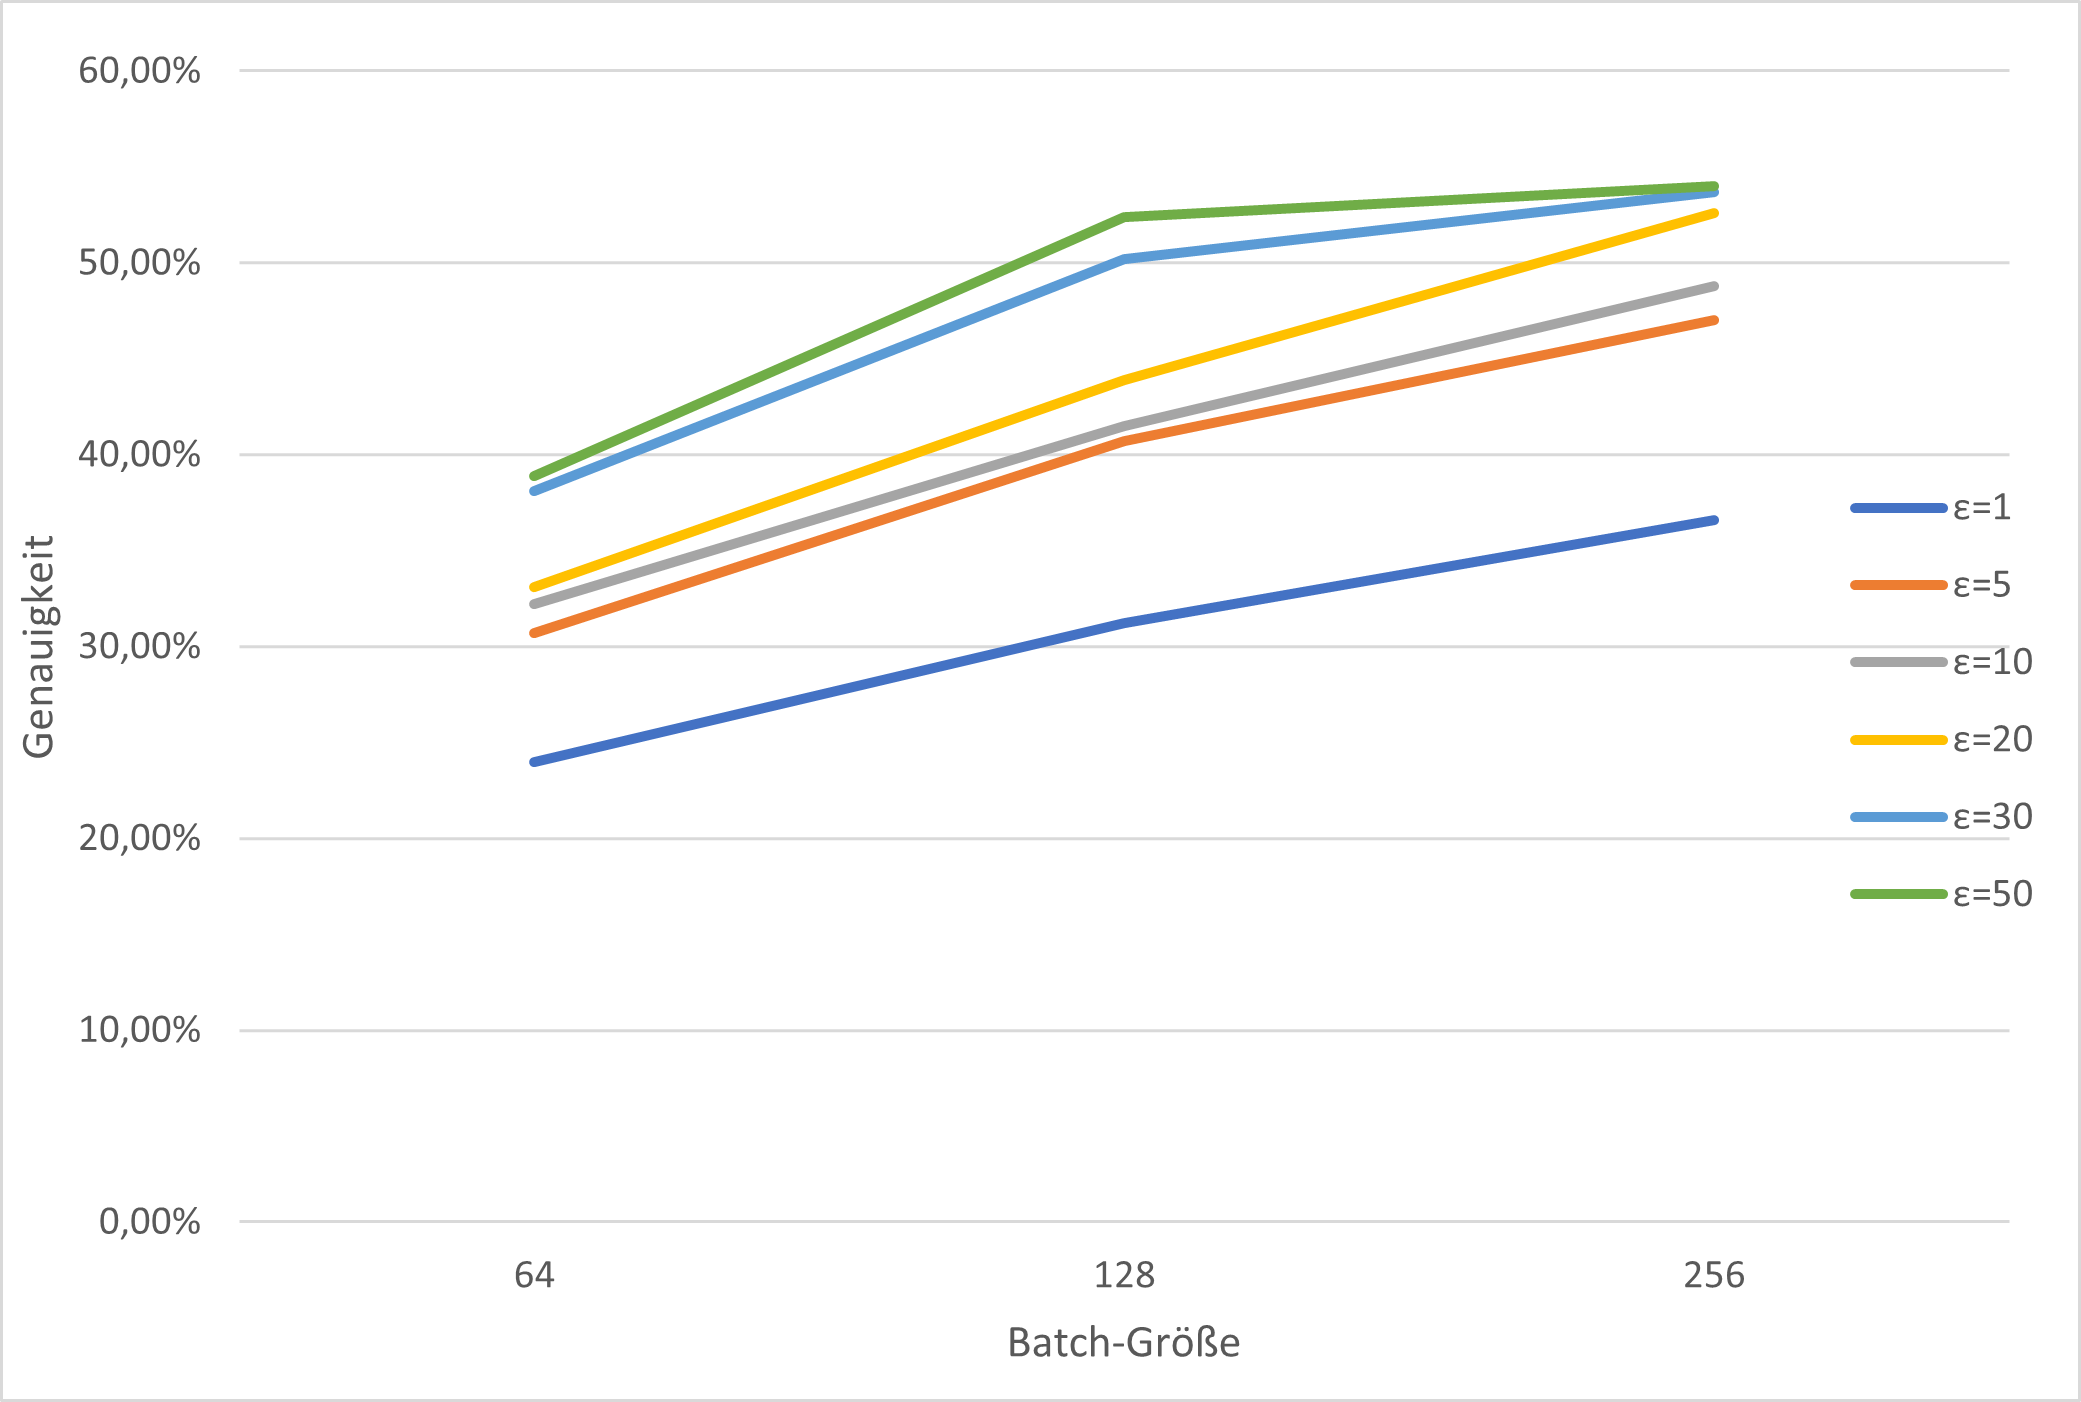
\includegraphics[width=14cm]{figures/results_cifar/cifar_batch_1.png}
    \caption{Auswirkung der Batch-Größe auf die Genauigkeit von CIFAR-10 Modellen}
    \label{fig:cifar-2}
\end{figure} 

Der zweite Versuch ähnelt dem ersten Versuch, jedoch wird die Datenaugmentierung nicht genutzt.
Dies sorgt dafür, dass die Genauigkeit der Modelle steigt. 
Abbildung \ref{fig:cifar_aug3} zeigt diesen Zusammenhang.
Die Modelle, dessen Genauigkeit dargestellt werden, werden jeweils 15 Epochen lang, mit einer Batch-Größe von 256, trainiert.
\begin{figure}[!htb]
    \centering
    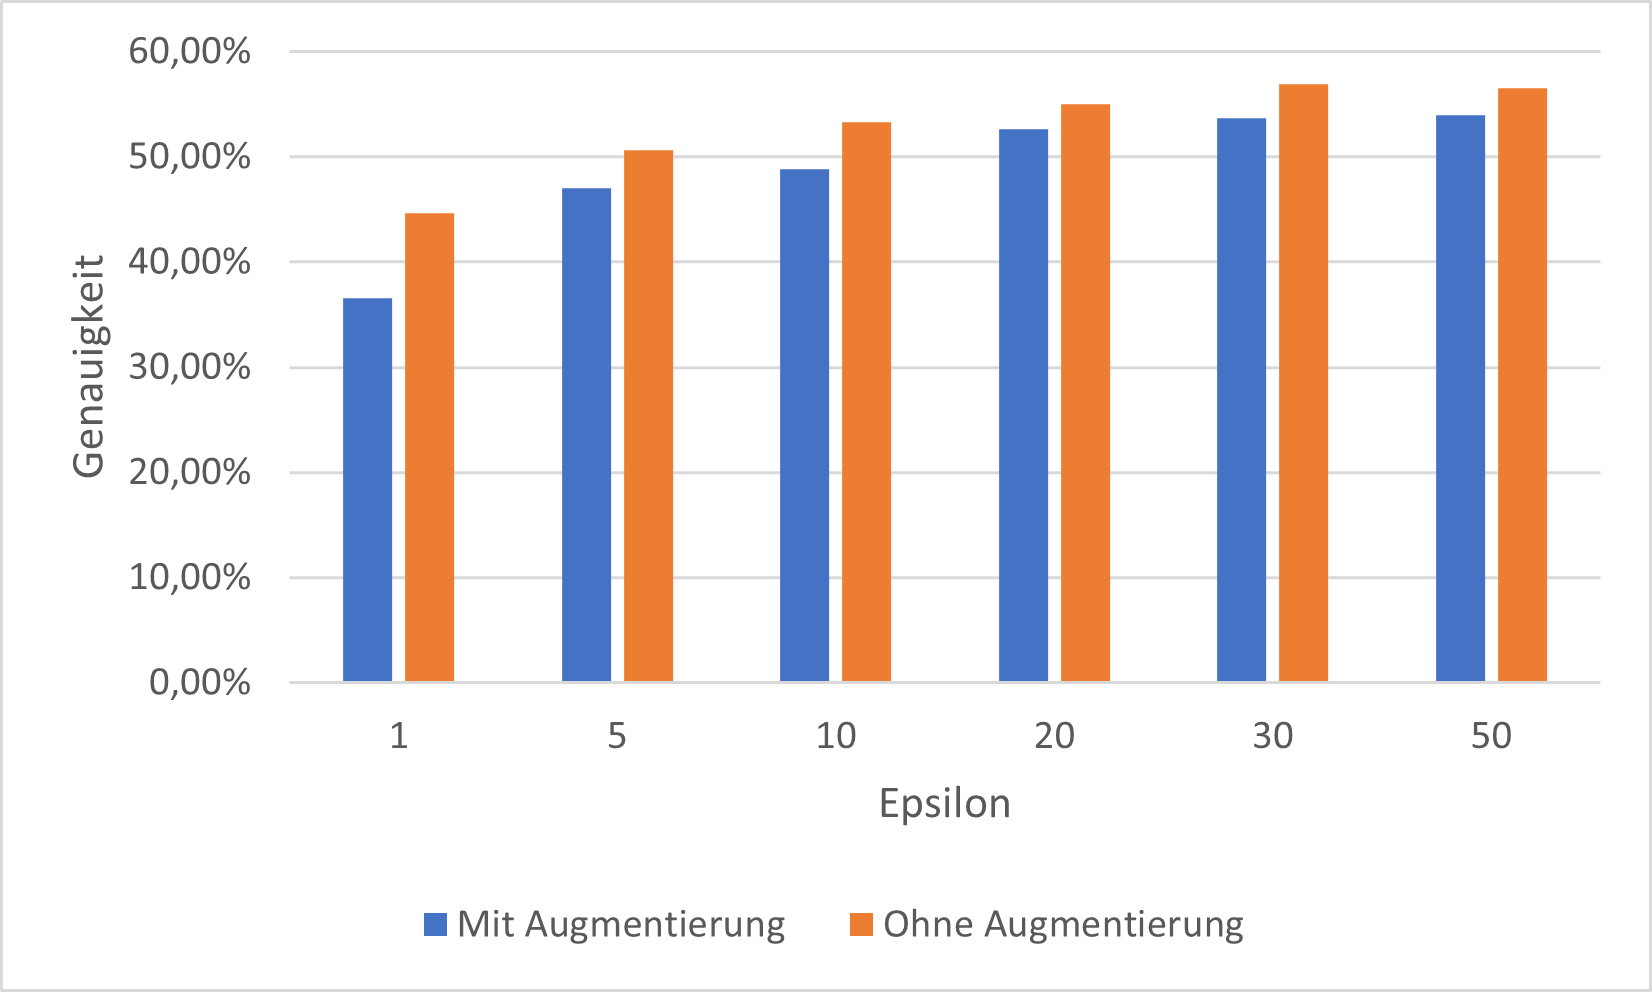
\includegraphics[width=14cm]{figures/results_cifar/cifar_aug3.png}
    \caption{Auswirkung von AutoAugment auf die Genauigkeit von CIFAR-10 Modellen}
    \label{fig:cifar_aug3}
\end{figure} 
Obwohl die Datenaugmentierung im zweiten Versuch nicht genutzt wird, kann das Modell 20 Epochen lang trainiert werden und hat dennoch eine steigende Genauigkeit.
Erst im Bereich zwischen 20 und 30 Epochen stagniert die Genauigkeit.
Im Vergleich zu dem Modell ohne DPSGD sind dies dennoch einige Epochen mehr.
Dies liegt daran, dass das Rauschen, genau wie die Datenaugmentierung, das Overfitting reduziert.

Der dritte Versuch gleicht dem zweiten Versuch, wobei hier der Wert der Clipping-Norm angepasst wurde.
Da die Clipping-Norm die Stärke des Rauschens beeinflusst, kann ein geringer Wert die Güte eines Modells erhöhen.
Wird der Wert jedoch zu gering gewählt, kann dies auch für den gegenteiligen Effekt sorgen, denn die Gradienten werden zu klein, damit das Modell in den geplanten Trainingsschritten konvergiert.
Um eine geeignete Clipping-Norm zu finden, wird das CIFAR-10 Modell über 5 Epochen trainiert, ohne Rauschen, jedoch mit unterschiedlichen Werten für das Clipping.
Dabei werden Zehnerpotenzen genutzt.
Der Wert wird immer um eine Zehnerpotenz reduziert, solange bis das Clipping einen leichten negativen Einfluss auf die Güte des Modells hat.
Die resultierende Zehnerpotenz ist in diesem Fall $10^{-5}$.
Da diese einen leichten negativen Einfluss auf das Modell hat, bedeutet dies, dass eine Vielzahl an Gradienten durch diesen Wert begrenzt wird.
Die Wahl der Clipping-Norm sollte auf diesen Wert fallen, oder einen minimal höheren Wert, welcher keinen Einfluss auf das Modell hat.
Durch die Wahl dieses geringen Werts wird auch die Stärke des Rauschens reduziert.
In diesem dritten Versuch wird die Clipping-Norm von $10^{-5}$ evaluiert.

Die Anpassung der Clipping-Norm wirkt sich nicht bei einer niedrigen Anzahl an Epochen aus.
Bei den CIFAR-10 Modellen, welche 15 Epochen lang trainiert werden, ist die Genauigkeit in etwa gleich, egal ob die Clipping-Norm bei 1 oder bei $10^{-5}$ liegt. 
Abbildung \ref{fig:cifar_clip1} zeigt den soeben beschriebenen Zusammenhang.
\begin{figure}[!htb]
    \centering
    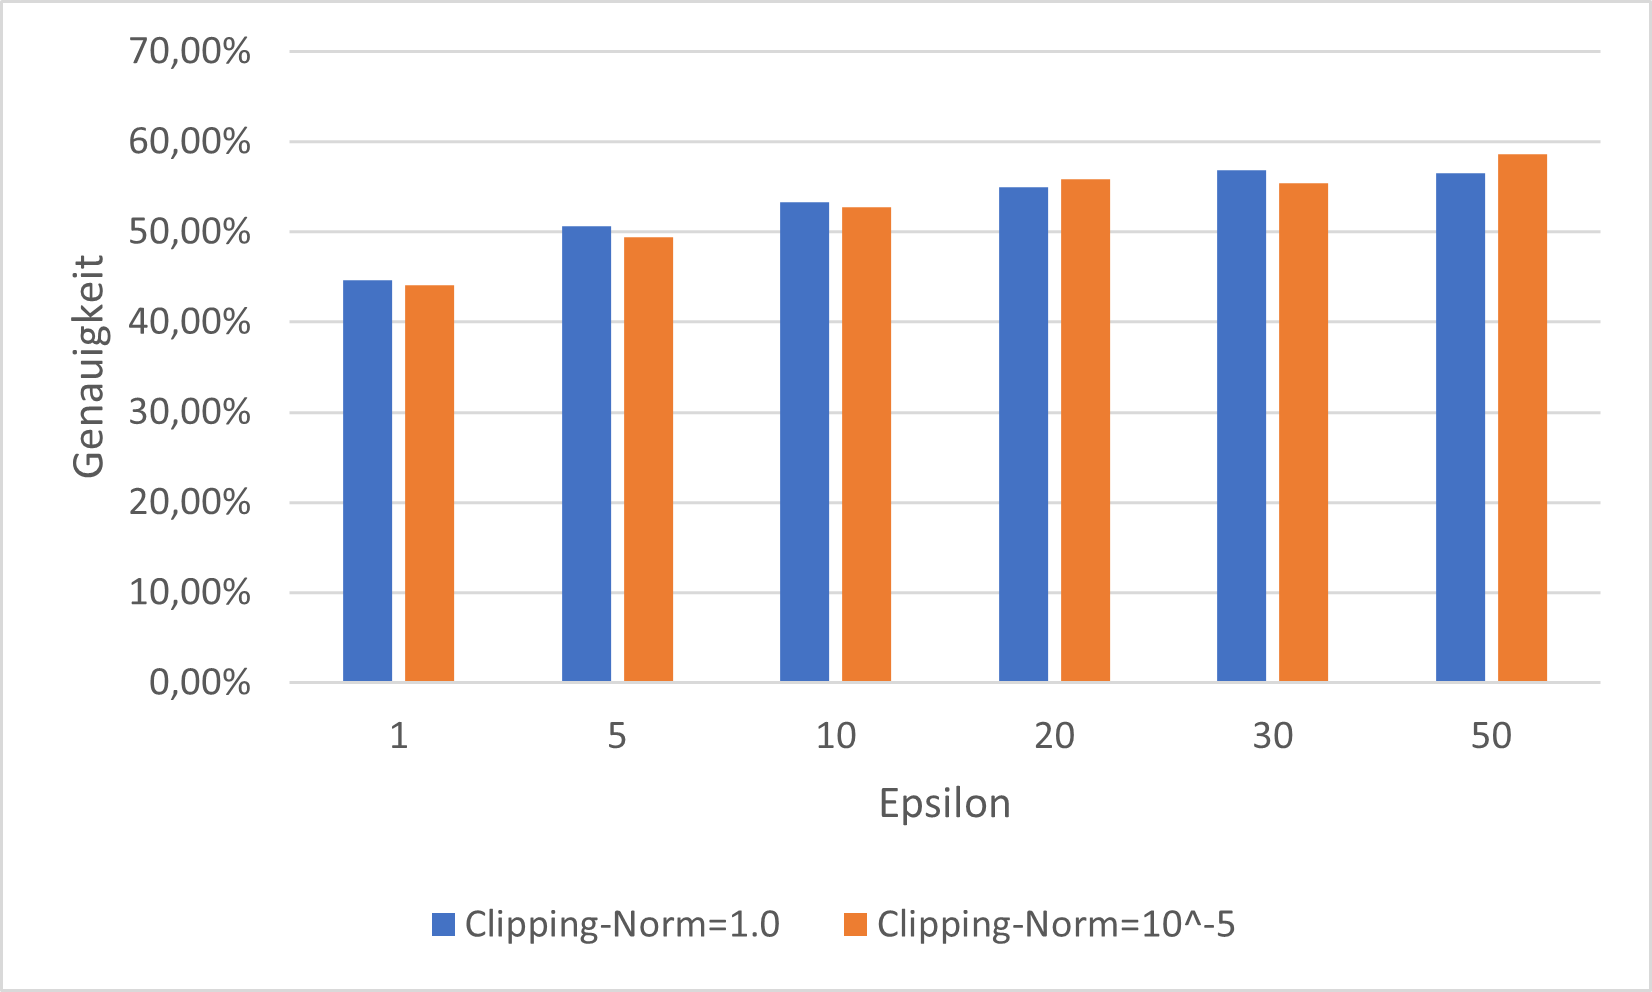
\includegraphics[width=14cm]{figures/results_cifar/cifar_clipp1.png}
    \caption{Auswirkung der Clipping-Norm auf die Güte von CIFAR-10 Modellen bei 15 Epochen Training}
    \label{fig:cifar_clip1}
\end{figure} 

Jedoch ermöglicht die geringere Clipping-Norm, mehr Epochen zu trainieren, ohne dass die Genauigkeit der Modelle stagniert. 
Dies liegt daran, dass die Gradienten mit kleiner Clipping-Norm kleiner sind, als die Gradienten mit großer Clipping-Norm. 
Somit werden mehr Trainingsschritte benötigt, um zu konvergieren. 
Außerdem ist die Stärke des Rauschens geringer, was ebenfalls die Güte des Modells verbessert.
Abbildung \ref{fig:cifar_clip2} zeigt den Vergleich zwischen einer hohen und einer niedrigen Clipping-Norm, wenn die Modelle jeweils 30 Epochen trainiert werden.

\begin{figure}[!htb]
    \centering
    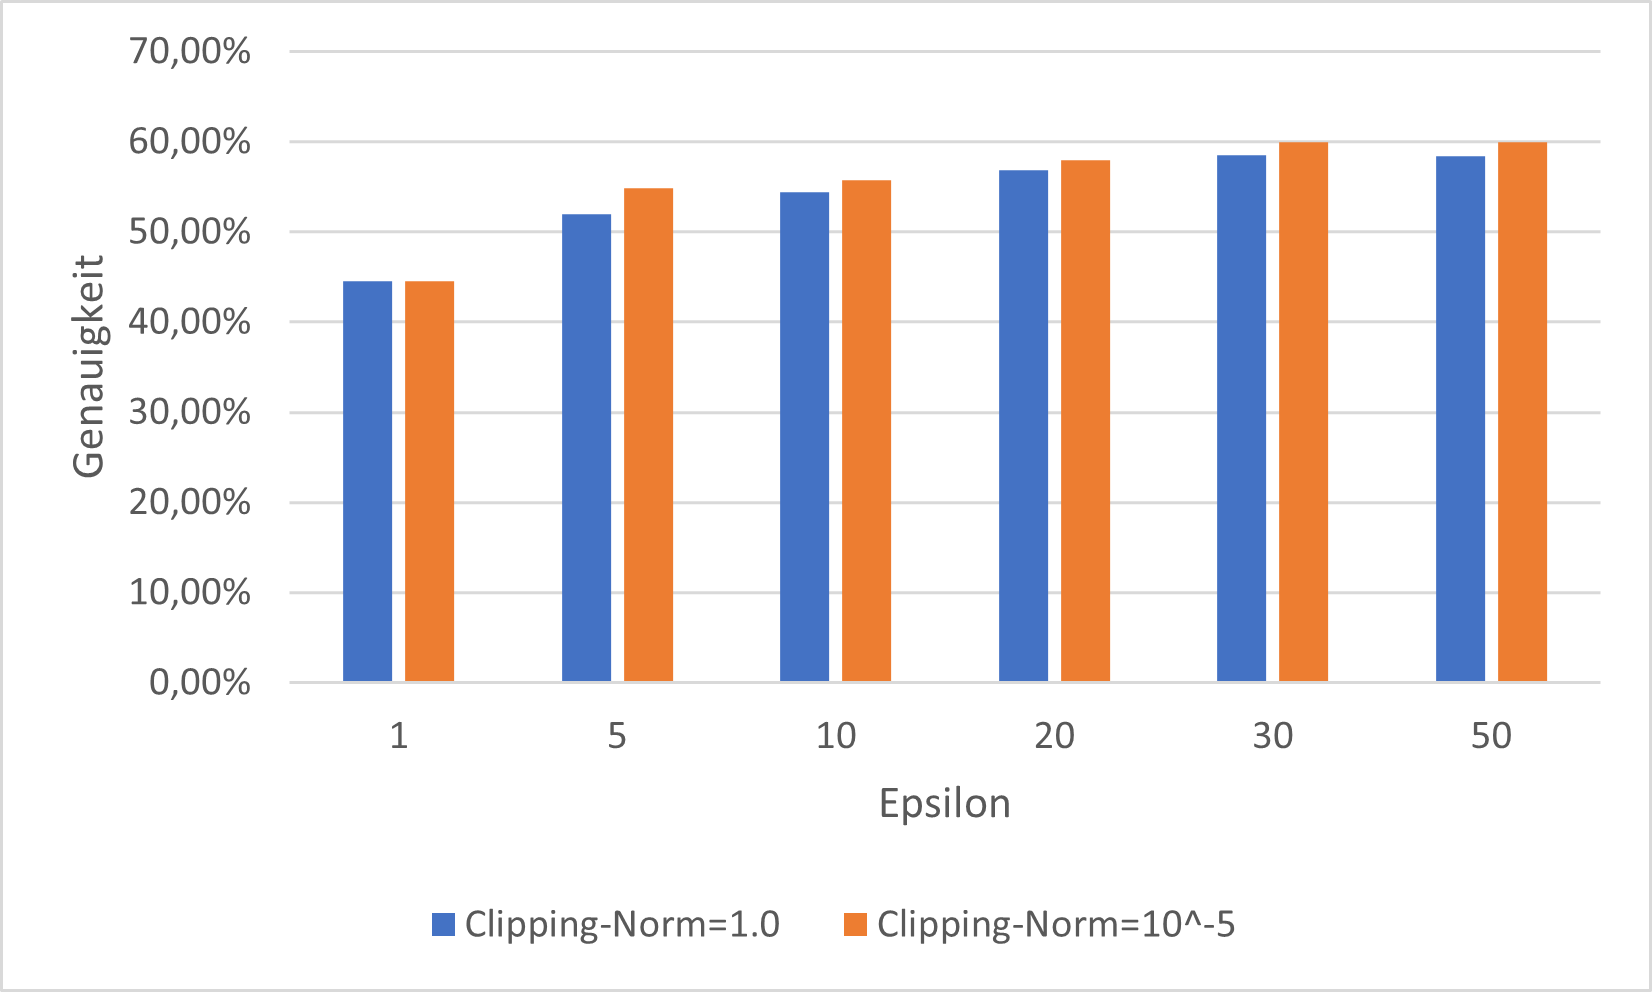
\includegraphics[width=14cm]{figures/results_cifar/cifar_clipp2.png}
    \caption{Auswirkung der Clipping-Norm auf die Güte von CIFAR-10 Modellen bei 30 Epochen Training}
    \label{fig:cifar_clip2}
\end{figure} 


Für das CIFAR-10 Modell mit DPSGD resultieren folgende Hyperparameter in einer optimalen Güte des Modells:
\begin{compactitem}
    \item \textbf{$\epsilon$-Wert des Privacy Budgets:} Der $\epsilon$-Wert korreliert mit der Güte des Modells. Kleine Werte schränken die Genauigkeit der Modelle ein, können aber die Vertraulichkeit besser schützen. Kapitel \ref{sec:bw_dp} gibt dabei einen Überblick über den Schutz der Modelle.
    \item \textbf{Batch-Größe:} Die Batch-Größe sollte möglichst groß gewählt werden. Hier kann ebenfalls der BatchMemoryManager von Opacus helfen, welcher eine virtuelle Batch-Größe ermöglicht, ohne den Speicher zu überlasten. Eine Batch-Größe von 512 bietet jedoch keinen Vorteil mehr gegenüber einer Batch-Größe von 256.
    \item \textbf{Anzahl Epochen:} Die Anzahl an Epochen ist höher als bei einem Modell ohne DPSGD. 
    Dies liegt daran, dass das Rauschen Overfitting abschwächt. Wird ein geringer Wert für die Clipping-Norm gewählt, können sogar noch mehr Epochen trainiert werden.
    Eine Epochenanzahl von 30 bietet immer noch eine steigende Genauigkeit, wohingegen ein Modell ohne DPSGD bereits nach 15 Epochen stagniert.
    \item \textbf{Datenaugmentierung:} Datenaugmentierung ist nicht notwendig und kann die Güte des Modells sogar verschlechtern.
    \item \textbf{Clipping-Norm:} Der Wert der Clipping-Norm sollte möglichst gering gewählt werden. Dies ermöglicht das Training von mehreren Epochen, wobei das Rauschen verringert wird.
\end{compactitem}

Tabelle \ref{tab:c10_dpsgd_res} zeigt, welche Genauigkeit mit verschiedenen $\epsilon$-Werten erreicht wird, wenn die Hyperparameter nach obigen Regeln optimiert werden.
\begin{table}[!htb]
\centering
\begin{tabular}{|l|l|l|l|l|}
\hline
\rowcolor[HTML]{CBCEFB} 
Epsilon  & \begin{tabular}[c]{@{}l@{}}Anzahl\\ Epochen\end{tabular} & Batch-Größe &Clipping-Norm & Genauigkeit \\ \hline

1  & 30 & 512 & $10^{-5}$  & 46,7 \% \\ \hline
5  & 30 & 512 & $10^{-5}$  & 55,0 \% \\ \hline
10 & 30 & 512 & $10^{-5}$  & 59,4 \% \\ \hline
20 & 30 & 512 & $10^{-5}$  & 60,5 \% \\ \hline
30 & 30 & 512 & $10^{-5}$  & 61,9 \% \\ \hline
50 & 30 & 512 & $10^{-5}$  & 63,2 \% \\ \hline
\end{tabular}
\caption{Genauigkeit von CIFAR-10 Modellen mit DPSGD}
\label{tab:c10_dpsgd_res}
\end{table}

\subsection{Hyperparameter ResNet-18 Modell}

Das originale ResNet-18 Modell ist für die Klassifikation des ImageNet Datenbestands trainiert. 
Da das Modell jedoch dafür genutzt werden soll, Merkmale aus Gesichtsbildern der CelebA Datenmenge zu erkennen, wird das Modell angepasst.
Dafür wird die ursprünglich letzte, vollständig verbundene Schicht durch eine neue, vollständig verbundene Schicht ausgetauscht, welche nur 40 Neuronen enthält.
Jedes Neuron steht dabei für eines der Merkmale.

Das ResNet-18 Modell bietet die Möglichkeit, die vortrainierten Gewichte zu nutzen, oder die Gewichte zufällig zu initialisieren.
Deshalb wird der Parameter \dq Vortrainiert\dq\ als zusätzlicher Hyperparameter evaluiert.
Dabei ist anzumerken, dass das Modell mit dem ImageNet Datenbestand vortrainiert ist, welches Bilder von Objekten enthält, jedoch nicht primär von Gesichtern.

Das vortrainierte ResNet-18 Modell ohne DPSGD erreicht eine Genauigkeit von 92,4 \% nach 10 Epochen mit Datenaugmentierung.
Wird stattdessen das nicht-vortrainierte Modell genommen, liegt die Genauigkeit bei 92,3 \%, also minimal darunter.
Das Deaktivieren der Datenaugmentierung hat jedoch einen größeren negativen Einfluss. 
Dadurch würde die Güte des Modells auf 91,0 \% für das vortrainierte und auf 90,1 \% für das nicht-vortrainierte Modell sinken.

Die Auswirkung der Hyperparameter des ResNet-18 Modells mit DPSGD ist gleich wie bei dem CIFAR-10 Modell.
Höhere Batch-Größen, eine niedrige Clipping-Norm und keine Nutzung von Datenaugmentierung sorgen für eine Verbesserung der Genauigkeit des Modells. 
Ob das Modell dabei vortrainiert oder nicht-vortrainiert ist, spielt eine untergeordnete Rolle und wirkt sich kaum auf die Genauigkeit der Modelle aus.
Anhang \ref{ch:ergebnisse_detail} enthält Tabellen mit detaillierten Messungen zu verschiedenen Hyperparametern von DPSGD.
Im Folgenden werden nur die besten Modelle betrachtet.

\begin{table}[!htb]
\centering
\begin{tabular}{|l|l|l|l|l|l|}
\hline
\rowcolor[HTML]{CBCEFB} 
Epsilon  & Clipping-Norm & Batch-Größe & \begin{tabular}[c]{@{}l@{}}Anzahl\\ Epochen\end{tabular} & \begin{tabular}[c]{@{}l@{}}Daten-\\ augmentierung\end{tabular} & Genauigkeit \\ \hline
$\infty$ & $\infty$      & 128         & 10                                                       & ja                                                             & 92,3 \%     \\ \hline
1        & $10^{-5}$     & 256         & 10                                                       & nein                                                           & 83,6 \%     \\ \hline
5        & $10^{-5}$      & 256         & 10                                                       & nein                                                           & 86,4 \%     \\ \hline
10       & $10^{-5}$     & 256         & 10                                                       & nein                                                           & 86,8 \%     \\ \hline
\end{tabular}
\caption{Übersicht der besten ResNet-18 Modelle mit DPSGD}
\label{tab:r18_best}
\end{table}

Tabelle \ref{tab:r18_best} zeigt dabei, was für eine Genauigkeit von Modellen erreicht werden kann, abhängig von unterschiedlichen $\epsilon$-Werten.
Die virtuelle Batch-Größe ist bei den DPSGD Modellen auf 256 gesetzt, wohingegen die physische Batch-Größe bei 64 liegt.
Der Wert für das Clipping wird auf $10^{-5}$ gesetzt, welcher einen leicht negativen Einfluss auf das Modell hat, bei einem $\epsilon$-Wert von unendlich.
Datenaugmentierung verschlechtert die Güte des Modells bei der Nutzung von DPSGD, weshalb diese nicht genutzt wird.
Bei einem $\epsilon$-Wert von 1 erreicht das Modell eine Genauigkeit von 83,6 \% und liegt damit absolut 8,7 \% unter dem Modell ohne DPSGD. 
Wird der $\epsilon$-Wert auf 10 erhöht, steigt die Genauigkeit auf 86,8 \% an. 
Damit hat dieses Modell nur 5,5 Prozentpunkte weniger Genauigkeit, als das Modell ohne DPSGD.

\subsection{Hyperparameter Vision Transformer Modell}

Das Vision Transformer Modell in PyTorch ist standardmäßig ebenfalls für die ImageNet-Datenmenge vortrainiert.
Dies bedeutet, dass hier ebenfalls die letzte, vollständig verbundene Schicht ausgetauscht wird, mit einer Schicht, welche 40 Neuronen, ein Neuron pro Merkmal, enthält.

Das vortrainierte Vision Transformer Modell ohne DPSGD erreicht eine Genauigkeit von 82,9 \% nach 10 Epochen mit Datenaugmentierung. 
Ohne Datenaugmentierung liegt die Genauigkeit bei 83,0 \% und damit minimal höher als mit Datenaugmentierung.
Wird jedoch das nicht-vortrainierte Vision Transformer Modell genutzt, sinken die Genauigkeiten auf 82,4 \% für das Modell ohne Datenaugmentierung und 82,3 \% für das Modell mit Datenaugmentierung.
Dies lässt schlussfolgern, dass die Nutzung von Datenaugmentierung kaum Einfluss auf das Modell ohne DPSGD hat.
Außerdem wird deutlich, dass das Vision Transformer Modell schlechter geeignet ist für die Merkmalserkennung aus Gesichtern, als das ResNet-18 Modell.

\begin{table}[!htb]
\centering
\begin{tabular}{llllll}
\hline
\rowcolor[HTML]{CBCEFB} 
\multicolumn{1}{|l|}{\cellcolor[HTML]{CBCEFB}Epsilon} & \multicolumn{1}{l|}{\cellcolor[HTML]{CBCEFB}Clipping-Norm} & \multicolumn{1}{l|}{\cellcolor[HTML]{CBCEFB}Batch-Größe} & \multicolumn{1}{l|}{\cellcolor[HTML]{CBCEFB}\begin{tabular}[c]{@{}l@{}}Anzahl\\ Epochen\end{tabular}} & \multicolumn{1}{l|}{\cellcolor[HTML]{CBCEFB}\begin{tabular}[c]{@{}l@{}}Daten-\\ augmentierung\end{tabular}} & \multicolumn{1}{l|}{\cellcolor[HTML]{CBCEFB}Genauigkeit} \\ \hline
\multicolumn{1}{|l|}{1}                               & \multicolumn{1}{l|}{1,0}                                   & \multicolumn{1}{l|}{16}                                  & \multicolumn{1}{l|}{5}                                                                                & \multicolumn{1}{l|}{ja}                                                                                     & \multicolumn{1}{l|}{79,4 \%}                             \\ \hline
\multicolumn{1}{|l|}{1}                               & \multicolumn{1}{l|}{$10^{-5}$}                             & \multicolumn{1}{l|}{128}                                 & \multicolumn{1}{l|}{5}                                                                                & \multicolumn{1}{l|}{nein}                                                                                   & \multicolumn{1}{l|}{80,0 \%}                             \\ \hline
                                                      &                                                            &                                                          &                                                                                                       &                                                                                                             &                                                          \\ \hline
\multicolumn{1}{|l|}{5}                               & \multicolumn{1}{l|}{1,0}                                   & \multicolumn{1}{l|}{16}                                  & \multicolumn{1}{l|}{5}                                                                                & \multicolumn{1}{l|}{ja}                                                                                     & \multicolumn{1}{l|}{78,8 \%}                             \\ \hline
\multicolumn{1}{|l|}{5}                               & \multicolumn{1}{l|}{$10^{-5}$}                             & \multicolumn{1}{l|}{128}                                 & \multicolumn{1}{l|}{5}                                                                                & \multicolumn{1}{l|}{nein}                                                                                   & \multicolumn{1}{l|}{80,0 \%}                             \\ \hline
                                                      &                                                            &                                                          &                                                                                                       &                                                                                                             &                                                          \\ \hline
\multicolumn{1}{|l|}{10}                              & \multicolumn{1}{l|}{1,0}                                   & \multicolumn{1}{l|}{16}                                  & \multicolumn{1}{l|}{5}                                                                                & \multicolumn{1}{l|}{ja}                                                                                     & \multicolumn{1}{l|}{79,4 \%}                             \\ \hline
\multicolumn{1}{|l|}{10}                              & \multicolumn{1}{l|}{$10^{-5}$}                             & \multicolumn{1}{l|}{128}                                 & \multicolumn{1}{l|}{5}                                                                                & \multicolumn{1}{l|}{nein}                                                                                   & \multicolumn{1}{l|}{80,3 \%}                             \\ \hline
\end{tabular}
\caption{Vergleich der Hyperparameter bei Vision Transformer Modellen}
\label{tab:vit_comp1}
\end{table}

Die Wahl der Hyperparameter hat außerdem bei diesem Modell weniger Einfluss auf die Genauigkeit, als bei den beiden vorherigen Modellen.
Tabelle \ref{tab:vit_comp1} zeigt, welche Genauigkeit die Vision Transformer Modelle mit DPSGD erreichen, wenn die Hyperparameter optimiert werden.
Dabei wird jeweils das vortrainierte Vision Transformer Modell genutzt.
Die unoptimierten Hyperparameter sind dabei eine Batch-Größe von 16, Nutzung von Datenaugmentierung und eine Clipping-Norm von 1,0.
Das Optimieren der Parameter erhöht die Batch-Größe auf 128, reduziert die Clipping-Norm auf $10^{-5}$ und deaktiviert die Nutzung von Datenaugmentierung.
Zusätzlich ist anzumerken, dass die DPSGD Modelle maximal für 5 Epochen trainiert wurden. 
Dies liegt daran, dass eine Epoche \ca 50 Minuten Zeit benötigt, was die Evaluierungsmöglichkeiten einschränkt.
Zudem gibt es keine signifikante Verbesserung der Genauigkeit bei einem Training des Vision Transformer Modells mit DPSGD von 3 Epochen und 5 Epochen.
Dies lässt andeuten, dass es ebenfalls keine signifikante Verbesserung der Genauigkeit bei 5 Epochen und 10 Epochen gibt.
Das Optimieren der Hyperparameter sorgt für eine absolute Verbesserung der Genauigkeit von 0,6, 1,2 und 0,8 Prozentpunkte, je nach Wahl von $\epsilon$.

\begin{table}[!htb]
\centering
\begin{tabular}{|l|l|l|l|l|l|}
\hline
\rowcolor[HTML]{CBCEFB} 
Epsilon  & Clipping-Norm & Batch-Größe & \begin{tabular}[c]{@{}l@{}}Anzahl\\ Epochen\end{tabular} & \begin{tabular}[c]{@{}l@{}}Daten-\\ augmentierung\end{tabular} & Genauigkeit \\ \hline
$\infty$ & $\infty$      & 64          & 10 & nein & 83,0 \%     \\ \hline
1        & $10^{-5}$     & 128         & 5 & nein & 80,0 \%     \\ \hline
5        & $10^{-5}$     & 128         & 5 & nein  & 80,0 \%     \\ \hline
10       & $10^{-5}$     & 128         & 5 & nein  & 80,3 \%     \\ \hline
\end{tabular}
\caption{Übersicht der besten Vision Transformer Modelle mit DPSGD}
\label{tab:vit_best}
\end{table}
Tabelle \ref{tab:vit_best} stellt die Genauigkeit des besten Vision Transformer Modells ohne DPSGD in Relation zu den Genauigkeiten der Vision Transformer Modelle mit DPSGD und optimierten Hyperparametern.
Die Genauigkeit des Modells ohne DPSGD ist bis zu 3 Prozentpunkte höher, als bei den Modellen mit DPSGD. 
Damit fällt Differenz der Genauigkeit von Modellen ohne DPSGD und mit DPSGD geringer aus, als bei den beiden vorherigen Modellarten.

\subsection{Handlungsempfehlung für die Wahl der Hyperparameter}

Die folgende Handlungsempfehlung zeigt, wie die Hyperparameter optimiert werden müssen, um die bestmögliche Güte eines Modells mit DPSGD zu erhalten. 
Der $\epsilon$-Wert wird hierbei außer Betracht gelassen.
Datenaugmentierung gilt es ebenfalls zu vermeiden.

\subsubsection*{Batch-Größe}
Da das Training mit DPSGD von Opacus mehr Speicher als das gleiche Training ohne DPSGD benötigt, muss zuerst eine geeignete Batch-Größe herausgefunden werden.
Dabei gibt es eine physische Batch-Größe, die Batch-Größe, die wirklich gleichzeitig in den Speicher passt, und eine virtuelle Batch-Größe, die größer sein kann.
Um die physische Batch-Größe zu finden, müssen die entsprechenden PyTorch Klassen in die Opacus Wrapper-Klassen eingebunden werden.
Die Parameter \bzgl dem Rauschen und Clipping können dabei ignoriert werden.
Anschließend kann ein Batch genutzt werden, um die Gradienten zu berechnen. 
An dieser Stelle ist es möglich, den Speicherverbrauch zu überwachen und so lange die Batch-Größe anzupassen, bis der Speicher optimal ausgenutzt ist.
Die virtuelle Batch-Größe kann größer gewählt werden, als die physische Batch-Größe.
Eine relativ große Batch-Größe sorgt dafür, dass die Werte des Rauschens sich ausgleichen. 
Eine zu große Batch-Größe hat jedoch auch negative Folgen.
Es empfiehlt sich eine Batch-Größe von 128, 256 oder 512.

\subsubsection*{Anzahl der Epochen}
Um die Stärke des Rauschens zu setzen, ist es wichtig, die geplante Anzahl an Epochen im Voraus zu kennen.
Die Anzahl der Epochen, welche bei einem Training mit DPSGD benötigt werden, können von dem Modell ohne DPSGD abgleitet werden.
Da das Hinzufügen von Rauschen als eine Art Regularisierung betrachtet werden kann, wird Overfitting durch DPSGD vermieden.
Somit könnten einige Epochen mehr trainiert werden, als bei dem Modell ohne DPSGD.
Die Evaluierung des ResNet-18 Modells und des Vision Transformer Modells haben jedoch kaum Verbesserungen bei einer hohen Anzahl an Epochen gezeigt.
Ein guter Richtwert ist es also, dass das Modell mit DPSGD für die gleiche Anzahl an Epochen trainiert wird, wie das Modell ohne DPSGD.

\subsubsection*{Clipping-Norm}
Der Wert des Clippings hat direkten Einfluss auf die Stärke des Rauschens und sollte deshalb klein gesetzt werden.
Ist der Wert jedoch zu klein, werden die Gradienten ebenfalls zu klein und das Modell wird nicht konvergieren.
Um eine ideale Clipping-Norm zu ermitteln, kann ein Modell für eine kleine Anzahl an Epochen mit DPSGD und Opacus trainiert werden. 
Der Wert des Rauschens wird dabei auf 0 gesetzt, wodurch sich ein $\epsilon$-Wert von unendlich ergibt.
Anschließend werden mehrere Modelle trainiert, welche jeweils eine unterschiedliche Zehnerpotenz als Clipping-Norm haben.
Die Clipping-Norm wird jeweils um eine Zehnerpotenz reduziert, solange bis ein Modell eine signifikant schlechtere Güte zeigt.
Dies bedeutet, dass diese Zehnerpotenz als Clipping-Norm eine signifikante Menge an Gradienten begrenzt und somit ein geeigneter Wert ist.


\section{Angriffe}\label{sec:exp_angriffe}

Das Ziel von Differential Privacy in Kombination mit neuronalen Netzen, ist es, Angriffe abzuschwächen. 
Im Folgenden wird anhand zweier Angriffe evaluiert, welchen Effekt die Nutzung von DPSGD hat.
Bei den zwei genutzten Angriffen handelt es sich um die Membership Inference Attacke und die Model Inversion Attacke.

\subsection{Membership Inference Attacke}

Die Membership Inference Attacke soll zeigen, ob ein Datensatz in der Trainingsdatenmenge eines Modells enthalten ist oder nicht.
Dazu werden Shadow Modelle genutzt, welche das anzugreifende Modell nachahmen. 
Die Vorhersagen der Shadow Modelle werden genutzt, um einen Meta-Klassifikator zu trainieren, welcher bestimmt, ob ein Datensatz bei einem Modell zum Training genutzt wurde.

Eine Besonderheit dieses Angriffs ist es, dass sowohl eine Black-Box, als auch eine White-Box Variante möglich ist.
Bei der White-Box Variante kennt der Angreifer die genaue Architektur des anzugreifenden Modells und kann die Architektur der Shadow Modell nachbilden.
In der Black-Box Variante, wird lediglich versucht, ähnliche Architekturen zu kreieren.
Dieses Experiment nutzt den White-Box Ansatz.
Dies liegt daran, dass es bei einem Black-Box Ansatz sein könnte, dass der Angreifer, durch Glück, eine nahezu identische Architektur der Shadow Modelle wählt. 
Somit kann ein Black-Box Ansatz theoretisch genauso effektiv sein, wie der White-Box Ansatz.

\subsubsection*{Membership Inference Attacke gegen das CIFAR-10 Modell}

Die CIFAR-10 Datenmenge besteht bereits aus einer Trainingsdatenmenge und einer Testdatenmenge, welche in Summe aus 60000 Datensätzen bestehen.
Für das Training der Shadow Modelle werden die beiden Datenmengen kombiniert.
Anschließend wird für jedes Shadow Modell zufällig eine Datenmenge, bestehend aus 50000 Datensätzen, für das Training ausgewählt.
Somit dienen die ausgewählten Daten nicht nur für das Training, sondern haben zusätzlich das Label \dq included\dq, wohingegen die nicht ausgewählten Daten das Label \dq excluded\dq\ erhalten.
Die Labels dienen im Anschluss dazu, die Datenmenge für den Meta-Klassifikator zu konstruieren.
Damit die Anzahl der beiden Labels in der Datenmenge gleich ist, werden von der genutzten Trainingsdatenmenge jedes Shadow Modells nur 10000 Datensätze gelabelt.
Somit entstehen pro Shadow Modell 20000 gelabelte Datensätze, jeweils 10000 mit dem Label \dq included\dq\ und 10000 mit dem Label \dq excluded\dq.

Der Meta-Klassifikator ist ein neuronales Netz, welches nur aus vollständig verbundenen Schichten besteht.
Dabei werden 10 Neuronen als Eingabe genutzt, je ein Neuron pro Vorhersagewahrscheinlichkeit einer Klasse, und ein Neuron als Ausgabe, welches das Label \dq included\dq\ oder \dq excluded\dq\ bestimmt.
Die Vorhersagewahrscheinlichkeiten, welche als Eingabe dienen, werden von den Shadow Modellen durch die Softmax-Funktion in den Wertebereich (0,1) übertragen, wobei eine Klasse einen Wert nahe 1 hat, die restlichen Klassen einen Wert von 0.

Die Trainingsdatenmenge und Testdatenmenge des CIFAR-10 Datenbestands könnte genutzt werden, um die Membership Inference Attacke zu bewerten, jedoch haben die Datenmengen eine ungleiche Anzahl an Datensätzen.
Würde der Meta-Klassifikator immer das Label \dq included\dq\ bestimmen, unabhängig des Inputs, dann entspräche dies einer Genauigkeit von \ca 83,3 \%, da die Anzahl der Datensätze in den beiden Datenmengen das gleiche Verhältnis haben.
Deshalb werden aus der Trainingsdatenmenge zufällig 10000 Datensätze ausgewählt. Diese, sowie die 10000 Datensätze der Testdatenmenge, dienen dann zur Evaluierung des Angriffs.
Dazu werden die Datensätze durch das anzugreifende Modell inferiert und die Vorhersagewahrscheinlichkeiten als Eingabe des Meta-Klassifikators genutzt.

Die Modelle, an welchen die Membership Inference Attacke getestet wird, sind die Modelle, welche in Kapitel \ref{sec:hyperparams} trainiert werden.
Dabei wird das beste Modell ohne DPSGD genutzt, sowie jeweils das Modell mit DPSGD, welches mit optimierten Hyperparametern trainiert wurde.

Tabelle \ref{tab:mi_cifar10_base} zeigt die Genauigkeit, welche der Meta-Klassifikator bei der Ausführung der Membership Inference Attacke gegen das CIFAR-10 Modell ohne DPSGD hat.
Dabei wurden eine unterschiedliche Anzahl an Shadow Modellen evaluiert, welche jeweils für 15 Epochen trainiert wurden und dadurch eine ähnliche Genauigkeit wie das originale Modell haben.
Die Genauigkeit des Angriffs ist bei 8,16 und 32 Shadow Modellen ähnlich.
Diese beträgt zwischen 57,4 \% und 58,9 \%.
\begin{table}[!htb]
\centering
\begin{tabular}{|l|l|l|}
\hline
\rowcolor[HTML]{CBCEFB} 
Epsilon & Anzahl Shadow Modelle & Genauigkeit des Angriff \\ \hline
$\infty$ & 8  & 58,0 \% \\ \hline
$\infty$ & 16 & 58,9 \% \\ \hline
$\infty$ & 32 & 57,4 \% \\ \hline
\end{tabular}
\caption{Membership Inference Angriff gegen CIFAR-10 Modell ohne DPSGD}
\label{tab:mi_cifar10_base}
\end{table}

Tabelle \ref{tab:mi_cifar10_part1} zeigt, wie sich die Genauigkeit des Angriffs durch die Nutzung von DPSGD ändert.
Bei allen Modellen mit DPSGD, hat die Membership Inference Attacke eine Genauigkeit zwischen 49,8 \% und 50,2 \%. 
Dadurch ist der Angriff weniger effektiv, als ohne die Nutzung von DPSGD.
\begin{table}[!htb]
\centering
\begin{tabular}{|l|l|l|}
\hline
\rowcolor[HTML]{CBCEFB} 
Epsilon & \begin{tabular}[c]{@{}l@{}}Anzahl \\ Shadow Modelle\end{tabular} & \begin{tabular}[c]{@{}l@{}}Genauigkeit \\ des Angriff\end{tabular} \\ \hline
$\infty$ & 32 & 57,4 \% \\ \hline
1        & 32 & 49,9 \% \\ \hline
5        & 32 & 49,8 \% \\ \hline
10       & 32 & 50,1 \% \\ \hline
20       & 32 & 50,2 \% \\ \hline
30       & 32 & 50,2 \% \\ \hline
50       & 32 & 50,0 \% \\ \hline
\end{tabular}
\caption{Membership Inference Angriff gegen CIFAR-10 Modelle mit DPSGD}
\label{tab:mi_cifar10_part1}
\end{table}

Das Problem des Angriffs ist jedoch, dass dieser nur minimal effektiv gegen ein Modell ohne DPSGD ist. 
Würde der Meta-Klassifikator zufällig ein Label wählen, würde dies einer Genauigkeit von \ca 50 \% entsprechen. 
Gegen ein Modell ohne DPSGD, erreicht der Meta-Klassifkator eine Genauigkeit von bis zu 58,9 \%, was eine Verbesserung ist.
Jedoch ermöglicht dies nicht, eine sachdienliche Aussage zu treffen.
Zusätzlich hat der Angreifer in der Regel keine Möglichkeit, den Angriff zu evaluieren. 
Dies liegt daran, dass der Angreifer keine Informationen \bzgl der genutzten Trainingsdatenmenge hat.
Die geringe Effektivität des Angriffs, sogar in der White-Box Variante, macht die Nutzung von DPSGD entbehrlich.

\subsubsection*{Membership Inference Attacke gegen das ResNet-18 Modell}
Die Membership Inference Attacke wird nur gegen das ResNet-18 Modell evaluiert, jedoch nicht gegen das Vision Transformer Modell.
Dies liegt an den benötigten Ressourcen, eine Vielzahl an Shadow Modellen zu trainieren, welche jeweils die Vision Transformer Architektur nutzen.

Das ResNet-18 Modell erkennt 40 Merkmale anhand von Gesichtsbildern des CelebA Datenbestand.
Im Gegensatz zu dem CIFAR-10 Modell wird nicht eine Klasse vorhergesagt, sondern 40 unabhängige Merkmale.
Dabei handelt es sich um eine sogenannte Multi-Label Klassifizierung, also einer Klassifikation bei welcher mehrere Labels vorhergesagt werden können.
Für das Modell sind diese 40 Labels unabhängig, fachlich sind jedoch einige dieser Labels verbunden.
So gibt es beispielsweise unterschiedliche Labels, welche für unterschiedliche Haarfarben stehen.
Da jede Person in dem Datenbestand eine Haarfarbe hat, hat maximal eines der Haarfarben-Labels den Wert 1, wohingegen die restlichen Haarfarben den Wert 0 haben.

Die Membership Inference Attacke gegen die ResNet-18 Modelle werden simultan zu den Angriffen gegen die CIFAR-10 Modelle durchgeführt.
Tabelle \ref{tab:mi_resnet18} zeigt die Genauigkeit des Angriffs gegen Modelle mit einem unterschiedlichen $\epsilon$-Wert.
Es wurden jeweils 8 Shadow Modelle trainiert und zum Labeln genutzt.
Der Angriff gegen das Modell ohne DPSGD hat eine Genauigkeit von 52,1 \% und ist damit nur minimal besser, als bei einer zufälligen Vorhersage.
Gegen Modelle die DPSGD benutzten ist der Angriff noch weniger effektiv und erreicht eine Genauigkeit von maximal 50,6 \%.

\begin{table}[!htb]
\centering
\begin{tabular}{|l|l|}
\hline
\rowcolor[HTML]{CBCEFB} 
Epsilon  & Genauigkeit des Angriff \\ \hline
$\infty$ & 52,1 \%                 \\ \hline
1        & 50,2 \%                 \\ \hline
5        & 50,6 \%                 \\ \hline
10       & 50,1 \%                 \\ \hline
\end{tabular}
\caption{Membership Inference Angriff gegen ResNet-18 Modelle mit DPSGD}
\label{tab:mi_resnet18}
\end{table}

\subsection{Model Inversion Attacke}

Bei der Model Inversion Attacke werden die Ausgaben eines Modells genutzt, um Rückschlüsse zu den Trainingsdaten zu ziehen.
Der hier evaluierte Angriff wird auch Reconstruction Attacke genannt. 
Ziel ist es, einen Datensatz aus dem Trainingsdatenbestand nachzubilden, lediglich anhand des Modells.
Hierfür wird ein Startbild in das Modell gegeben, welches zu Beginn lediglich eine Ansammlung von zufälligen Pixeln ist.
Die Vorhersage des Modells wird anschließend mit einer Verlustfunktion durch das Modell backpropagiert, jedoch werden nicht die Gewichte des Modells angepasst, sondern die Werte des Startbildes.
Dadurch verändert sich das Bild, bis es das gewünschte Label zeigt.
Der Vorgang wird dabei iterativ wiederholt.
Zusätzlich wird in jedem Schritt das Bild mittels eines Autoencoders entrauscht, sodass sich die zufällige Ansammlung von Pixeln zu einem möglichst realistischen Bild umwandeln.
Der iterative Vorgang kann nach einer festgelegten Anzahl an Wiederholungen gestoppt werden, oder bis das rekonstruierte Bild den gewünschten Detailgrad erreicht hat.

\subsubsection*{Model Inversion Attacke gegen CIFAR-10 Modell}
Um die Model Inversion Attacke durchzuführen, wurde zu Beginn ein Autoencoder trainiert.
Dieser soll Bilder entrauschen, \dahe das Rauschen aus Bildern entfernen und diese realistischer werden lassen.
Als Ausgabe des Modells werden daher die Bilder des CIFAR-10 Trainingsdatenbestand genutzt, wobei die Eingabe jeweils eine verrauschte Version dieses Bildes ist.
Die verrauschten Bilder können erzeugt werden, indem ein zufälliges Rauschen über jedes Pixel hinzugefügt wird.

Der Autoencoder hat die gleiche Eingabedimension wie Ausgabedimension, welche $32\times32\times3$ Pixeln entspricht.
In einer verdeckten Schicht ist die Dimension jedoch niedriger, welche dafür sorgt, dass das Modell in dieser nur einen Teil der Bildinformationen zwischenspeichern kann.
Zum Verkleinern der Dimensionen werden Faltungsschichten und Pooling-Operationen genutzt.
Das Vergrößern der Dimension wird mit transponierten Faltungsschichten ausgeführt.
Transponierte Faltungsschichten funktionieren simultan zu normalen Faltungsschichten, jedoch wird zuvor das Bild um interpolierte Pixel erweitert. 
Abbildung \ref{fig:autoencoder_cifar} zeigt, welchen Effekt der Autoencoder auf verrauschte Bilder ausübt.
Der linke Teil der Abbildung zeigt ein originales Bild aus der CIFAR-10 Datenmenge. 
Dieses ist der Klasse \dq Schiff\dq\ untergeordnet.
Der mittlere Teil der Abbildung zeigt dabei die zufällig verrauschte Version dieses Bildes.
Das Schiff ist dabei kaum zu erkennen, da viele Pixel des Bildes eine andere Farbe angenommen haben.
Der rechte Teil der Abbildung zeigt, wie die Ausgabe des Autoencoders bei Eingabe des verrauschten Bildes aussieht.
Das Schiff ist wieder erkennbar und das Bild ähnelt dem originalen Bild.

\begin{figure}[!htb]
\centering
\begin{subfigure}[h]{0.3\textwidth}
  \centering
  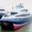
\includegraphics[width=\linewidth]{figures/autoencoder_cifar/1.jpg}
  \caption{Originales Bild}
\end{subfigure}
\begin{subfigure}[h]{0.3\textwidth}
  \centering
  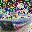
\includegraphics[width=\linewidth]{figures/autoencoder_cifar/2.jpg}
  \caption{Verrauschtes Bild}
\end{subfigure}
\begin{subfigure}[h]{0.3\textwidth}
  \centering
  
\includegraphics[width=\linewidth]{figures/autoencoder_cifar/3.jpg}
  \caption{Ausgabe Autoencoder}
\end{subfigure}
\caption{Autoencoder CIFAR-10 Datenbestand}
\label{fig:autoencoder_cifar}
\end{figure}

Wird die Model Inversion Attacke gegen das CIFAR-10 Modell ohne DPSGD ausgeführt, kann kein Bild rekonstruiert werden.
Parameter wie der Optimizer, die Lernrate oder die Verlustfunktion wurden angepasst, jedoch führte dies zu keiner Verbesserung des Angriffs 
Zusätzlich wurden unterschiedliche Methoden der Initialisierung des Startbildes gewählt.
Ebenfalls wurden evaluiert, den Angriff einige Iterationen ohne den Autoencoder durchzuführen.
Keine der Anpassungen sorgte für eine Verbesserung des Angriffs.

Abbildung \ref{fig:moder_inv_c10} zeigt, das Ergebnis einer Model Inversion Attacke, wenn ein Bild mit dem Label \dq Schiff\dq\ nachgebildet werden soll.
Das linke Bild entspricht dem initialen Startbild, bei dem alle Farbwerte jeweils mit dem Wert 0,5 befüllt werden. 
Dies entspricht einem grauen Bild.
Das mittlere Bild zeigt, wie sich das Bild nach einigen Iterationen des Angriffs ohne Autoencoder verändert hat.
Dabei handelt es sich um zufällig aussehende Pixel, jedoch sagt das CIFAR-10 Modell bei diesem Bild das gewünschte Label \dq Schiff\dq\ vorher.
Das rechte Bild zeigt das Ergebnis des Angriffs, nachdem das Bild für weitere Iterationen angepasst wurde und pro Iteration mit dem Autoencoder angepasst wurde.
Das entstandene Bild besteht primär aus gräulichen Pixeln, welche eine Musterung aufweisen, die vermutlich vom Autoencoder stammt.
Es ist kein Schiff zu erkennen.
\begin{figure}[!htb]
\centering
\begin{subfigure}[h]{0.3\textwidth}
  \centering
  
\includegraphics[width=\linewidth]{figures/autoencoder_cifar/mi_cifar_start_grey.jpg}
  \caption{Initiales Bild\\jeder Wert=0,5}
\end{subfigure}
\begin{subfigure}[h]{0.3\textwidth}
  \centering
  
\includegraphics[width=\linewidth]{figures/autoencoder_cifar/mi_cifar_mid_grey.jpg}
  \caption{Anpassung \\ohne Autoencoder}
\end{subfigure}
\begin{subfigure}[h]{0.3\textwidth}
  \centering
  
\includegraphics[width=\linewidth]{figures/autoencoder_cifar/mi_cifar_finish_grey.png}
  \caption{Anpassung \\mit Autoencoder}
\end{subfigure}
\caption{Model Inversion Attacke gegen CIFAR-10}
\label{fig:moder_inv_c10}
\end{figure}

\subsubsection*{Model Inversion Attacke gegen ResNet-18 Modell}

Die Model Inversion Attacke gegen das ResNet-18 Modell erfolgt simultan zu der Attacke gegen das CIFAR-10 Modell.
Zuerst wird ein Autoencoder trainiert, welcher das Rauschen von Bildern der CelebA Datenmenge entfernt.
Abbildung \ref{fig:autoencoder_celeba} zeigt, wie ein verrauschtes Bild mittels des Autoencoders wieder entrauscht werden kann.
Der Output des Autoencoders, also das entrauschte Bild, zeigt das Gesicht einer Person, jedoch ist das Bild weniger scharf als das originale Bild.

\begin{figure}[!htb]
\centering
\begin{subfigure}[h]{0.3\textwidth}
  \centering
  
\includegraphics[width=\linewidth]{figures/autoencoder_r18/faces_autoencoder1.jpg}
  \caption{Originales Bild}
\end{subfigure}
\begin{subfigure}[h]{0.3\textwidth}
  \centering
  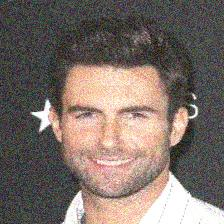
\includegraphics[width=\linewidth]{figures/autoencoder_r18/faces_autoencoder2.jpg}
  \caption{Verrauschtes Bild}
\end{subfigure}
\begin{subfigure}[h]{0.3\textwidth}
  \centering
  
\includegraphics[width=\linewidth]{figures/autoencoder_r18/faces_autoencoder3.jpg}
  \caption{Ausgabe Autoencoder}
\end{subfigure}
\caption{Autoencoder CelebA Datenbestand}
\label{fig:autoencoder_celeba}
\end{figure}

Die Model Inversion Attacke ist ebenfalls gegen das ResNet-18 Modell ohne DPSGD nicht effektiv.
Abbildung \ref{fig:moder_inv_cr18} zeigt dabei das Ergebnis einer Rekonstruktion. 
Die Labels, nach welchen das Bild rekonstruiert werden soll, entstammen dem Beispielbild aus Abbildung \ref{fig:autoencoder_celeba}.
Als Startbild dient hier wieder ein Bild, bei welchem jeder Farbwert auf den Wert 0,5 gesetzt ist.
Dieses wurde für einige Iterationen durch die Backpropagation des Modells angepasst, jedoch vorerst ohne Autoencoder.
Hier entsteht eine zufällige Ansammlung an Pixeln, welche jedoch vom Modell die gewünschten Labels vorhergesagt bekommt.
Nach einigen weiteren Iterationen, sowie zusätzlichen Anpassungen mittels des Autoencoders, entsteht wieder ein relativ gräuliches Bild.
Dieses besitzt ebenfalls eine Musterung, welche vermutlich durch den Autoencoder entstanden ist.
\begin{figure}[!htb]
\centering
\begin{subfigure}[h]{0.3\textwidth}
  \centering
  
\includegraphics[width=\linewidth]{figures/autoencoder_r18/faces_mi1.jpg}
  \caption{Initiales Bild\\jeder Wert=0,5}
\end{subfigure}
\begin{subfigure}[h]{0.3\textwidth}
  \centering
  
\includegraphics[width=\linewidth]{figures/autoencoder_r18/faces_mi2.jpg}
  \caption{Anpassung ohne\\Autoencoder}
\end{subfigure}
\begin{subfigure}[h]{0.3\textwidth}
  \centering
  
\includegraphics[width=\linewidth]{figures/autoencoder_r18/faces_mi3.png}
  \caption{Anpassung mit\\Autoencoder}
\end{subfigure}
\caption{Model Inversion Attacke gegen ResNet-18 Modell}
\label{fig:moder_inv_cr18}
\end{figure}
\section{Zusammenfassung der Experimente}

PyTorch stellt mit Opacus eine Bibliothek zur Verfügung, welche die Nutzung von DPSGD durch einige Wrapper-Klassen ermöglicht.
Opacus bietet über die Klasse \textbf{PrivacyEngine} einen simplen Weg, die PyTorch Objekte entsprechend umzuwandeln. 
Anschließend erfolgt das Training mit normalem PyTorch Code, weshalb die Nutzung von DPSGD mit Opacus kein aufwendiges Refactoring benötigt.
Da jedoch die Funktionsweise von PyTorch durch Opacus angepasst wird, steigt der Speicherverbrauch, sowie die Trainingsdauer einer Epoche (Kaptiel \ref{sec:opacu_implementierung}). 

Durch die richtige Wahl von Hyperparametern kann die Güte von neuronalen Netzen mit DPSGD optimiert werden.
Dazu sollte eine möglichst große Batch-Größe, ein geringer Wert der Clipping-Norm und eine verhältnismäßig hohe Anzahl an Trainingsepochen gewählt werden.
Ein höherer $\epsilon$-Wert sorgt ebenfalls für eine bessere Güte des Modells.
Die Hyperparameter wurden anhand von drei Modellen evaluiert:
\begin{compactitem}
    \item \textbf{CIFAR-10 Modell}: Das CIFAR-10 Modell ist ein neuronales Netz, welches eine ResNet-Architektur mit 10 Schichten nutzt und den CIFAR-10 Datenbestand in 10 unterschiedliche Klassen einteilt. Bei der ResNet-Architektur handelt es sich um ein neuronales Netz mit Faltungsschichten, welches zusätzlich sogenannte Skip Connections nutzt.
    \item \textbf{ResNet-18 Modell}: Das ResNet-18 Modell ist ein neuronales Netz mit 18 Schichten, welches ebenfalls die ResNet-Architektur nutzt. Dieses Modell erkennt 40 Merkmale aus Bildern von menschlichen Gesichtern.
    \item \textbf{Vision Transformer Modell}: Das Vision Transformer Modell erkennt ebenfalls 40 Merkmale aus Bildern von menschlichen Gesichtern.
    Jedoch basiert dieses auf der Transformer-Architektur, welche Embeddings, Aufmerksamkeitsmechanismen und Encoder nutzt.
\end{compactitem}
Die Differenz der Genauigkeit des CIFAR-10 Modells mit DPSGD und ohne DPSGD fällt dabei am größten aus. 
Bei einem $\epsilon$-Wert von 10, sinkt die Genauigkeit von 82,9 \% ohne DPSGD auf eine Genauigkeit von 59,4 \%.
Die Differenz fällt bei dem ResNet-18 Modell und bei dem Vision Transformer Modell geringer aus. 
Bei dem ResNet-18 Modell sinkt die Genauigkeit bei einem $\epsilon$-Wert von 10 um 5,5 Prozentpunkte.
Die Genauigkeit des Vision Transformer Modells sinkt bei einem $\epsilon$-Wert von 10 nur um 2,7 Prozentpunkte (Kapitel \ref{sec:hyperparams}).

Die Wahl von $\epsilon$ und der damit einhergehende Schutz ist abhängig von der benötigten Sicherheit.
Jedoch wird gezeigt, dass die Membership Inference Attacke und die Model Inversion Attacke bei den genutzten Use Cases nicht effektiv ist. 
Sogar bei den Modellen ohne DPSGD sind die Angriffe unwirksam (Kapitel \ref{sec:exp_angriffe}).











\chapter{Diskussion}

\section{Handlungsempfehlung anhand der Ergebnisse}
Sicherheit versus Performance/Accuracy

\section{Offene Forschungbereiche}

\section{Zusammenfassung der Ergebnisse}


%\appendix
%\include{content/a1_supplemental}

\backmatter
\listoffigures
\cleardoublepage

\listoftables
\cleardoublepage

\renewcommand{\lstlistlistingname}{Auflistungen}
\lstlistoflistings
\cleardoublepage

\printbibliography

\end{document}
